%% For normal draft builds (figs undisplayed hence fast compile)
%\documentclass[hyperpdf,nobind,draft,oneside]{hepthesis}
%\documentclass[hyperpdf,nobind,draft,twoside]{hepthesis}

%% For short draft builds (breaks citations by necessity)
%\documentclass[hyperpdf,nobind,draft,hidefrontback]{hepthesis}

%%For Cambridge soft-bound version
\documentclass[hyperpdf,bindnopdf]{hepthesis}
%% For Cambridge hard-bound version (must be one-sided)
%\documentclass[hyperpdf,oneside]{hepthesis}

%% Load special font packages here if you wish
%\usepackage{lmodern}
\usepackage{mathpazo}
\usepackage{subfig}
\usepackage{amsmath}
\usepackage{mwe}
\usepackage{upgreek}
%\usepackage{euler}

%% Put package includes etc. into preamble.tex for convenience
\usepackage{xspace}
\usepackage{tikz}
\usepackage{morefloats,subfig,afterpage}
\usepackage{mathrsfs} % script font
\usepackage{verbatim}

%% Using Babel allows other languages to be used and mixed-in easily
%\usepackage[ngerman,english]{babel}
\usepackage[english]{babel}
\selectlanguage{english}

%% Citation system tweaks
\usepackage{cite}
% \let\@OldCite\cite
% \renewcommand{\cite}[1]{\mbox{\!\!\!\@OldCite{#1}}}

%% Maths
% TODO: rework or eliminate maybemath
\usepackage{abmath}
\DeclareRobustCommand{\mymath}[1]{\ensuremath{\maybebmsf{#1}}}
% \DeclareRobustCommand{\parenths}[1]{\mymath{\left({#1}\right)}\xspace}
% \DeclareRobustCommand{\braces}[1]{\mymath{\left\{{#1}\right\}}\xspace}
% \DeclareRobustCommand{\angles}[1]{\mymath{\left\langle{#1}\right\rangle}\xspace}
% \DeclareRobustCommand{\sqbracs}[1]{\mymath{\left[{#1}\right]}\xspace}
% \DeclareRobustCommand{\mods}[1]{\mymath{\left\lvert{#1}\right\rvert}\xspace}
% \DeclareRobustCommand{\modsq}[1]{\mymath{\mods{#1}^2}\xspace}
% \DeclareRobustCommand{\dblmods}[1]{\mymath{\left\lVert{#1}\right\rVert}\xspace}
% \DeclareRobustCommand{\expOf}[1]{\mymath{\exp{\!\parenths{#1}}}\xspace}
% \DeclareRobustCommand{\eexp}[1]{\mymath{e^{#1}}\xspace}
% \DeclareRobustCommand{\plusquad}{\mymath{\oplus}\xspace}
% \DeclareRobustCommand{\logOf}[1]{\mymath{\log\!\parenths{#1}}\xspace}
% \DeclareRobustCommand{\lnOf}[1]{\mymath{\ln\!\parenths{#1}}\xspace}
% \DeclareRobustCommand{\ofOrder}[1]{\mymath{\mathcal{O}\parenths{#1}}\xspace}
% \DeclareRobustCommand{\SOgroup}[1]{\mymath{\mathup{SO}\parenths{#1}}\xspace}
% \DeclareRobustCommand{\SUgroup}[1]{\mymath{\mathup{SU}\parenths{#1}}\xspace}
% \DeclareRobustCommand{\Ugroup}[1]{\mymath{\mathup{U}\parenths{#1}}\xspace}
% \DeclareRobustCommand{\I}[1]{\mymath{\mathrm{i}}\xspace}
% \DeclareRobustCommand{\colvector}[1]{\mymath{\begin{pmatrix}#1\end{pmatrix}}\xspace}
\DeclareRobustCommand{\Rate}{\mymath{\Gamma}\xspace}
\DeclareRobustCommand{\RateOf}[1]{\mymath{\Gamma}\parenths{#1}\xspace}

%% High-energy physics stuff
\usepackage{abhep}
\usepackage{hepnames}
\usepackage{hepunits}
\DeclareRobustCommand{\arXivCode}[1]{arXiv:#1}
\DeclareRobustCommand{\CP}{\ensuremath{\mathcal{CP}}\xspace}
\DeclareRobustCommand{\CPviolation}{\CP-violation\xspace}
\DeclareRobustCommand{\CPv}{\CPviolation}
\DeclareRobustCommand{\LHCb}{LHCb\xspace}
\DeclareRobustCommand{\LHC}{LHC\xspace}
\DeclareRobustCommand{\LEP}{LEP\xspace}
\DeclareRobustCommand{\CERN}{CERN\xspace}
\DeclareRobustCommand{\bphysics}{\Pbottom-physics\xspace}
\DeclareRobustCommand{\bhadron}{\Pbottom-hadron\xspace}
\DeclareRobustCommand{\Bmeson}{\PB-meson\xspace}
\DeclareRobustCommand{\bbaryon}{\Pbottom-baryon\xspace}
\DeclareRobustCommand{\Bdecay}{\PB-decay\xspace}
\DeclareRobustCommand{\bdecay}{\Pbottom-decay\xspace}
\DeclareRobustCommand{\BToKPi}{\HepProcess{ \PB \to \PK \Ppi }\xspace}
\DeclareRobustCommand{\BToPiPi}{\HepProcess{ \PB \to \Ppi \Ppi }\xspace}
\DeclareRobustCommand{\BToKK}{\HepProcess{ \PB \to \PK \PK }\xspace}
\DeclareRobustCommand{\BToRhoPi}{\HepProcess{ \PB \to \Prho \Ppi }\xspace}
\DeclareRobustCommand{\BToRhoRho}{\HepProcess{ \PB \to \Prho \Prho }\xspace}
\DeclareRobustCommand{\X}{\thesismath{X}\xspace}
\DeclareRobustCommand{\Xbar}{\thesismath{\overline{X}}\xspace}
\DeclareRobustCommand{\Xzero}{\HepGenParticle{X}{}{0}\xspace}
\DeclareRobustCommand{\Xzerobar}{\HepGenAntiParticle{X}{}{0}\xspace}
\DeclareRobustCommand{\epluseminus}{\Ppositron\!\Pelectron\xspace}
\DeclareRobustCommand{\protonproton}{\Pproton\APantiproton\xspace}



\usepackage{xcolor} % for \Yoshi command below
%% Command to print or not print comments from Yoshi
%\DeclareRobustCommand{\Yoshi}[2]{{{}}} % ignore me completely version
%\DeclareRobustCommand{\Yoshi}[2]{{#1}} % believe everything I say version
\DeclareRobustCommand{\Yoshi}[2]{{\color[RGB]{111,0,158}{{#1}\footnote{\color[RGB]{111,0,158}#2}}}} % full words of wisdom version

%% You can set the line spacing this way
%\setallspacing{double}
%% or a section at a time like this
%\setfrontmatterspacing{double}


%% Define the thesis title and author
\title{Measurement of the charged-current inclusive muon-neutrino interaction cross-section on lead using the T2K ND280 electromagnetic calorimeters}
\author{Dominic Brailsford}

%% Doc-specific PDF metadata
\makeatletter
\@ifpackageloaded{hyperref}{%
\hypersetup{%
  pdftitle = {Measurement of the charged-current inclusive muon-neutrino interaction cross-section on lead using the T2K ND280 electromagnetic calorimeters},
  pdfsubject = {Dominic Brailsford's PhD thesis},
  pdfkeywords = {T2K, neutrino, cross-section},
  pdfauthor = {\textcopyright\ Dominic Brailsford}
}}{}
\makeatother



%% Start the document
\begin{document}

%% Define the un-numbered front matter (cover pages, rubrik and table of contents)
%\begin{frontmatter}
%  %% Title
\titlepage[TODO] {
  A thesis submitted to Imperial College London\\ for the degree of Doctor of Philosophy}

%% Abstract
\begin{abstract}%[\smaller \thetitle\\ \vspace*{1cm} \smaller {\theauthor}]
  %\thispagestyle{empty}
  To write
  \end{abstract}


%% Declaration
\begin{declaration}
  This dissertation is the result of my own work, except where explicit
  reference is made to the work of others, and has not been submitted
  for another qualification to this or any other university. This
  dissertation does not exceed the word limit for the respective Degree
  Committee.
  \vspace*{1cm}
  \begin{flushright}
    Dominic Brailsford
  \end{flushright}
\end{declaration}


%% Acknowledgements
\begin{acknowledgements}
  Something about my supervisor \dots
\end{acknowledgements}


%% Preface
\begin{preface}
  \noindent
  This thesis describes my analysis of the $\nu_\mu$ charged-current cross-section on lead using the 
  T2K near detector electromagnetic calorimeters.

\end{preface}

%% ToC
\tableofcontents


%% Strictly optional!
\frontquote{%
  These chickens jackin' my style.
}%
  {Fergie}
%% I don't want a page number on the following blank page either.
\thispagestyle{empty}

%\end{frontmatter}

%% Start the content body of the thesis
\begin{mainmatter}

%Set the section numbering to 3 layers deep
\setcounter{secnumdepth}{3}

  %% Actually, more semantic chapter filenames are better, like "chap-bgtheory.tex"
  %\chapter{Introduction}
\label{chap:Introduction}

%% Restart the numbering to make sure that this is definitely page #1!
\pagenumbering{arabic}

The field of neutrino physics is currently undergoing a revolution.  With its tenuous postulation~\cite{PauliOpenLetter} acting as a future omen, the neutrino's mark on history would not become apparent from its discovery~\cite{Cowan20071956, PhysRevLett.9.36, Kodama2001218}, but rather from a spate of surprising discoveries at the end of the 20th century~\cite{PhysRevLett.81.1562, PhysRevLett.87.071301, PhysRevLett.90.021802} which conclusively proved that the Standard Model, while very successful, was incomplete.  This revelation was experimental proof of Maki, Nagakawa and Sakata's extension~\cite{Maki01111962} to Pontecorvo's theory of neutrino oscillation ~\cite{Pontecorvo} with the inclusion of the Mikheyev-Smirnov-Wolfenstein (MSW) effect~\cite{PhysRevD.17.2369,Mikheev:1986gs}.  The findings were groundbreaking as the underlying theory requires massive neutrinos, which is in direct contradiction to the Standard Model.  The, now, standard theory of neutrino oscillation defines three neutrino flavours and three neutrino masses.  However, the map between flavour and mass is not one-to-one, but rather a rotation of mass space onto flavour space.  The main consequence of this rotation is that the flavour eigenstates are a superposition of mass eigenstates, namely
\begin{equation}
\ket{\nu_\alpha} = \sum^{3}_{i=k}U^{\ast}_{\alpha k}\ket{\nu_k},
\label{eq:NeutrinoEigenstates}
\end{equation}
where $\alpha \in \{e,\mu, \tau\}$, $\nu_k$ are the neutrino mass eigenstates and $U^{\ast}_{\alpha k}$ is an element of a unitary rotation matrix which is known as the PMNS mixing matrix.  As there are 3 mass and flavour eigenstates, the PMNS matrix is a $3\times3$ matrix and is often parameterised as 
\begin{equation}
U \equiv
\begin{pmatrix}
1 & 0 & 0 \\
0 & c_{23} & s_{23} \\
3 & -s_{23} & c_{23}
\end{pmatrix}
\begin{pmatrix}
c_{13} & 0 & s_{13}e^{-i\delta} \\
0 & 1 & 0 \\
-s_{13}e^{i\delta} & 0 & c_{13} 
\end{pmatrix}
\begin{pmatrix}
c_{12} & s_{12} & 0 \\
-s_{12} & c_{12} & 0 \\
0 & 0 & 1
\end{pmatrix}
,
\label{eq:PMNSMatrix}
\end{equation}
where $c_{ij} \equiv \cos\theta_{ij}$ and $s_{ij} \equiv \sin\theta_{ij}$. $\theta_{ij}$ are known as the mixing angles which parameterise how strong mixings between the flavour and mass eigenstates are and $\delta$ is a CP violating phase.  The most surprising observable feature of this mechanism is the non-zero probability to detect a neutrino of specific flavour which was created at source in a different flavour state.  By propagating the mass eigenstates through time, one can arrive at this probability which has the following form 
\begin{equation}
P(\nu_\alpha \rightarrow \nu_\beta) = |\braket{\nu_\beta|\nu\left(t\right)}|^2 = |U_{\beta k} e^{-iE_{k}t}  U^{\ast}_{\alpha k}|^2,
\label{eq:NeutrinoOscillationProbability}
\end{equation}
where $\nu\left(t\right)$ is the time-dependent neutrino mass eigenstate and $E_k$ is the energy of the $\nu_k$.  For an accelerator-based neutrino oscillation experiment, the beam will be $\nu_\mu$ dominated.  So, the $\nu_\mu$ survival probability, $P(\nu_\mu \rightarrow \nu_\mu)$, and $\nu_e$ appearance probability, $P(\nu_\mu \rightarrow \nu_e)$, have are typically of interest and can be approximated in the following forms
\begin{equation}
P(\nu_\mu \rightarrow \nu_\mu) \approx 1 - \cos^{4}\theta_{13}\sin^{2}2\theta_{23}\sin^2\left(1.27\frac{\Delta m^{2}_{23}}{\left(\textrm{eV}^2\right)}\frac{L}{\left(\textrm{km}\right)}\frac{\left(\textrm{GeV}\right)}{E}\right)
  \label{eq:MuonNeutrinoSurvivalProbability}
\end{equation}
\begin{equation}
P(\nu_\mu \rightarrow \nu_\mu) \approx \sin^{2}2\theta_{13}\sin^{2}\theta_{23}\sin^2\left(1.27\frac{\Delta m^{2}_{23}}{\left(\textrm{eV}^2\right)}\frac{L}{\left(\textrm{km}\right)}\frac{\left(\textrm{GeV}\right)}{E}\right),
  \label{eq:ElectronNeutrinoAppearanceProbability}
\end{equation}
where $\Delta m^{2}_{ij} \equiv m^{2}_{i} - m^{2}_{j}$, $L$ is the distance the neutrino propagates and $E$ is the energy of the neutrino.

\section{The state of the field}
\label{sec:StateOfTheField}
Data provided from a wide range of experiments show excellent agreement with the theory of neutrino oscillation and with a 3 flavour neutrino picture.  Global fits applied to the data provided by these experiments gives best fit values for the oscillation parameters, which are summarised in table~\ref{table:NeutrinoOscillationParameterValues}~\cite{Agashe:2014kda}.
\begin{table}
  \begin{tabular}{l c }
    Parameter & best-fit $(\pm1\sigma)$ \\ \hline \hline
    $\Delta m^2_{12}$ [$10^{-5}\textrm{eV}^2$] & $7.54^{+0.26}_{-0.22}$ \\
    $|\Delta m^2|$ [$10^{-3}\textrm{eV}^2$] & $2.43\pm0.06$ $(2.36\pm0.06)$ \\
    $\sin^2\theta_{12}$ & $0.308\pm0.017$ \\
    $\sin^2\theta_{23}$, $\Delta m^2 > 0$ & $0.437^{+0.033}_{-0.023}$ \\
    $\sin^2\theta_{23}$, $\Delta m^2 < 0$ & $0.455^{+0.039}_{-0.031}$ \\
    $\sin^2\theta_{13}$, $\Delta m^2 > 0$ & $0.0234^{+0.0020}_{-0.0019}$ \\
    $\sin^2\theta_{13}$, $\Delta m^2 < 0$ & $0.0240^{+0.019}_{-0.022}$ \\
    $\sin^2\theta_{13}$, $\Delta m^2 < 0$ & $0.0240^{+0.019}_{-0.022}$ \\
    $\delta/\pi$ ($2\sigma$ range quoted) & $1.39^{+0.38}_{-0.27}$ $(1.31^{+0.29}_{-0.33})$ \\
  \end{tabular}
  \caption{The best-fit values of the 3-neutrino oscillation parameters. $\Delta m^2 \equiv m^2_3 - \left(m^2_2 - m^2_1\right)/2$. The values (values in brackets) correspond to $m_1 < m_2 < m_3$ ($m_3 < m_1 < m_2$)~\cite{Agashe:2014kda}.}
  \label{table:NeutrinoOscillationParameterValues}
\end{table}
The experiments which provided the data inputs to the global fit generally fall into one of four catagories, with each catagory sensitive to a different subset of the neutrino oscillation parameters.
\newline
\newline
Solar neutrino experiments detect neutrinos generated in the core of the Sun as a result of nuclear reaction chains.  Such experiments are primarily sensitive to $\theta_{12}$ and $\Delta m^{2}_{12}$ which are often referred to as the solar mixing parameters.  The final state neutrinos created in the Sun's core are MeV-scale $\nu_e$ but, because of propagation through the core's surrounding matter, the MSW effect results in a highly pure state of $\nu_2$ at the Sun's surface.  As $\nu_2$ is a mass eigenstate, no oscillation occurs between the surface of the Sun and the Earth.  Homestake~\cite{0004-637X-496-1-505}, SAGE~\cite{PhysRevC.80.015807} and SNO~\cite{PhysRevLett.87.071301} are examples of such experiments.
\newline
\newline
Reactor neutrino experiments measure $\bar{\nu}_e$ disappearance provided by inverse $\beta$ decay in nuclear reactors with an average neutrino energy of 3~MeV.  The baseline for oscillations varies between experiments, but a baseline of around 1~km provides excellent sensitivity to $\theta_{13}$. Examples of reactor experiments are CHOOZ~\cite{CHOOZ}, Double CHOOZ~\cite{Abe201366}, Daya Bay~\cite{PhysRevLett.108.171803} and RENO~\cite{PhysRevLett.108.191802}.
\newline
\newline
Atmospheric neutrino experiments detect neutrinos which are produced from $\pi$ and $K$ mesons, created bycosmic rays interactions with the upper atmosphere of the Earth, decay.  The neutrinos produced are a mixture of $\nu_\mu$, $\bar{\nu}_\mu$, $\nu_e$ and $\bar{\nu}_e$.  Because the cosmic ray flux is fairly uniform, atmospheric neutrino experiments are exposed to neutrinos from all directions, which results in a very wide range of oscillation baselines.  The oscillation parameters that such experiments are sensitive to are $\theta_23$ and $\Delta m^2_{13}$. Super-Kamiokande~\cite{PhysRevLett.81.1562} is an example of an atmospheric neutrino experiment. 
\newline
\newline
Accelerator neutrino experiments produce beams of high purity $\nu_\mu$ (or $\bar{\nu_\mu}$) at GeV-scale energy with wide ranging baselines which are generally $\mathcal{O}\left(100~\textrm{km}\right)$.  The highly man-made nature of such experiments allows almost complete control over $L/E$ allowing careful tuning of parameter sensitivity.  Accelerator neutrino experiments are generally sensitive to $\theta_{13}$, $\theta_{23}$, $\Delta m^{2}_{13}$ and $\delta$. K2K~\cite{PhysRevD.74.072003}, MINOS~\cite{PhysRevLett.97.191801}, T2K~\cite{PhysRevLett.112.061802} and NO$\nu$A~\cite{Ayres:2004js}are examples of such experiments.

  %%\begin{sidewaysfigure}
%  \begin{center}
%  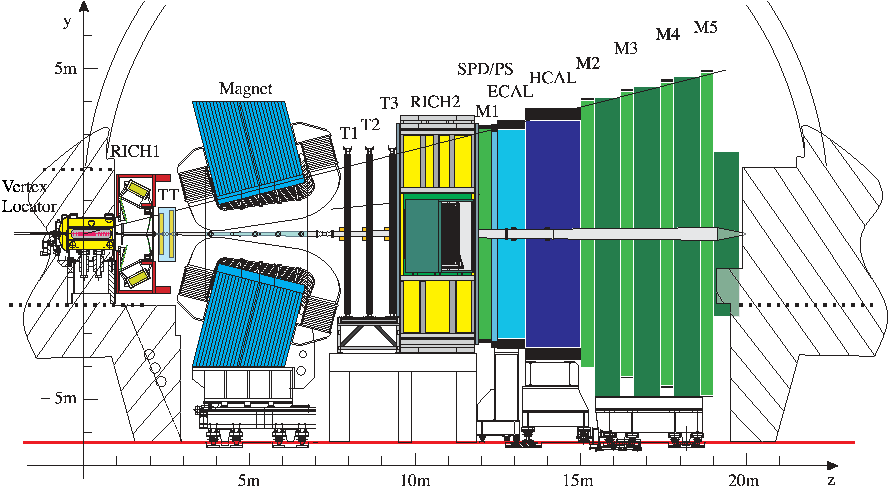
\includegraphics[width=0.8\textheight]{lhcb-detector-cross-section}
%  \caption[Cross-section view of \LHCb, cut in the non-bending $y$--$z$ plane]%
%    {Cross-section view of \LHCb, cut in the non-bending $y$--$z$ plane.}
%  \label{fig:LHCbCrossSection}
%  \end{center}
%\end{sidewaysfigure}



\chapter{Neutrino interactions with atomic nuclei}
\label{chap:NeutrinoInteractionsAtomicNuclei}
The neutrino is a strictly weakly\Yoshi{-}{hyphen}interacting particle.  This has difficult implications for any experiment aiming to study neutrinos as particle detectors generally rely on the electromagnetic force.  In fact, the only proven method of neutrino detection is to utilise a high mass target in which the neutrinos can interact\Yoshi{}{was ` with'}.  Generally speaking, charged particles are produced by this interaction which can be detected by the usual means.  The collected information from these charged final states can then be used to infer information about the incident neutrino.  \Yoshi{All neutrino experiments}{no they don't! Tritium decay mass measurements and the helicity measurement, the Homestake experiment -- all these are neutrino experiments that use other methods!} rely on this method and so any attempted measurements (e.g. \Yoshi{$\delta$)}{this is not a ``measurement''} rely on our understanding \Yoshi{of}{ was `on'} neutrino interactions with atomic nuclei.  Our understanding of such processes is encompassed in the models we use to simulate the interactions.

\section{Neutrino interactions at the GeV-scale}
\label{sec:NeutrinoInteractionsGeVScale}
As the neutrino is weakly interacting, there are two channels available to a neutrino interacting with a nucleon: the Charge Current (CC) interaction in which a W boson is exchanged and the Neutral Current (NC) interaction in which a Z boson is exchanged.  For neutrino energies below $\sim$1~GeV, the neutrino-hadron interactions are largely Quasi-Elastic (QE)~\cite{RevModPhys.84.1307}.  In such an interaction, the incident neutrino scatters of the nucleon as if it were a single particle, rather than with one of the nucleon's constituent partons.  In the case of a CCQE interaction, the neutrino is converted into its charged lepton equivalent and the target neutron converted to a proton.  In the specific case of an incident $\nu_\mu$, the interaction takes the following form
\begin{equation}
\nu_\mu n \rightarrow \mu^- p.
\label{eq:CCQEInteraction}
\end{equation}
For NCQE interactions, the incident neutrino remains after the interaction has occurred and no nucleon conversion takes place.  Because of this fact, the target nucleon in a NCQE interaction need not be a neutron.  So, for $\nu_\mu$ NCQE interactions, there are two channels available
\begin{equation}
\nu_\mu n \rightarrow \nu_\mu n,
\label{eq:NCQEInteractionNeutronTarget}
\end{equation}
\begin{equation}
\nu_\mu p \rightarrow \nu_\mu p.
\label{eq:NCQEInteractionProtonTarget}
\end{equation}
The two kinds of QE interaction are shown in Fig.~\ref{fig:QEFD}\Yoshi{}{In the figure, the W isn't really a W$^+$; it could be going either way in time. You can only call it a W}.
\begin{figure}%
  \centering
  \subfloat[CCQE.]{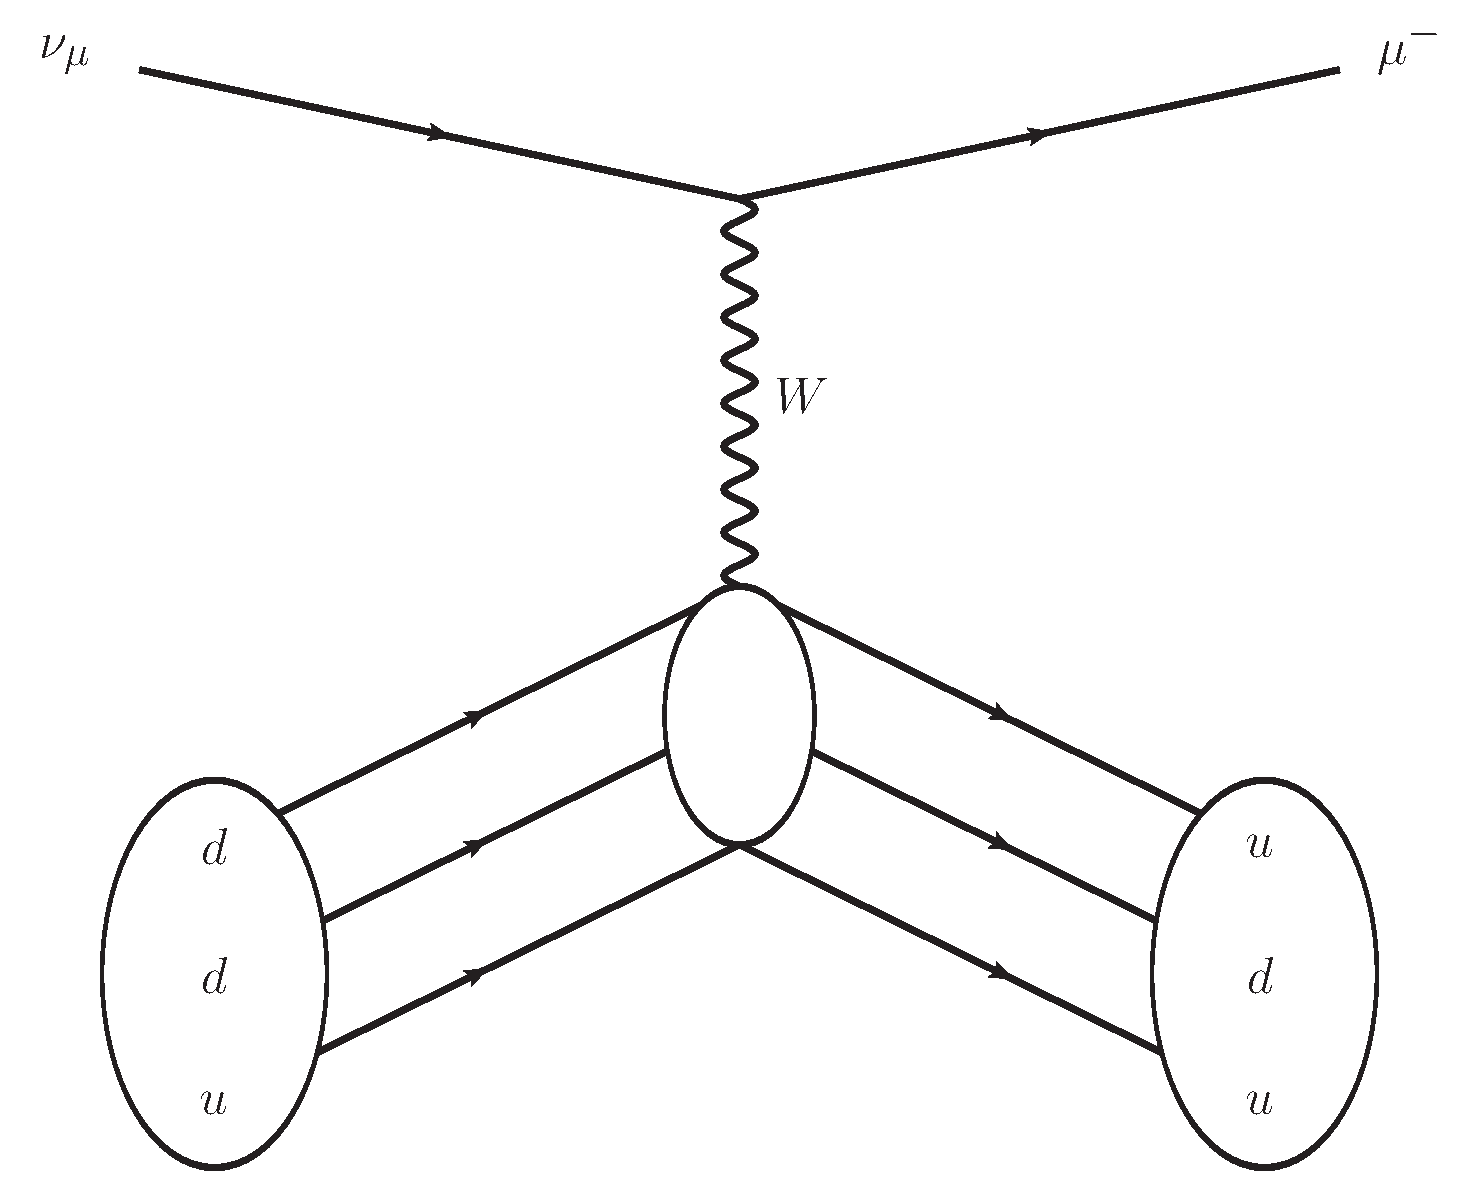
\includegraphics[width=8cm]{images/neutrino_interactions/CCQE_FD.eps} \label{fig:CCQEFD}}
  \subfloat[NCQE.]{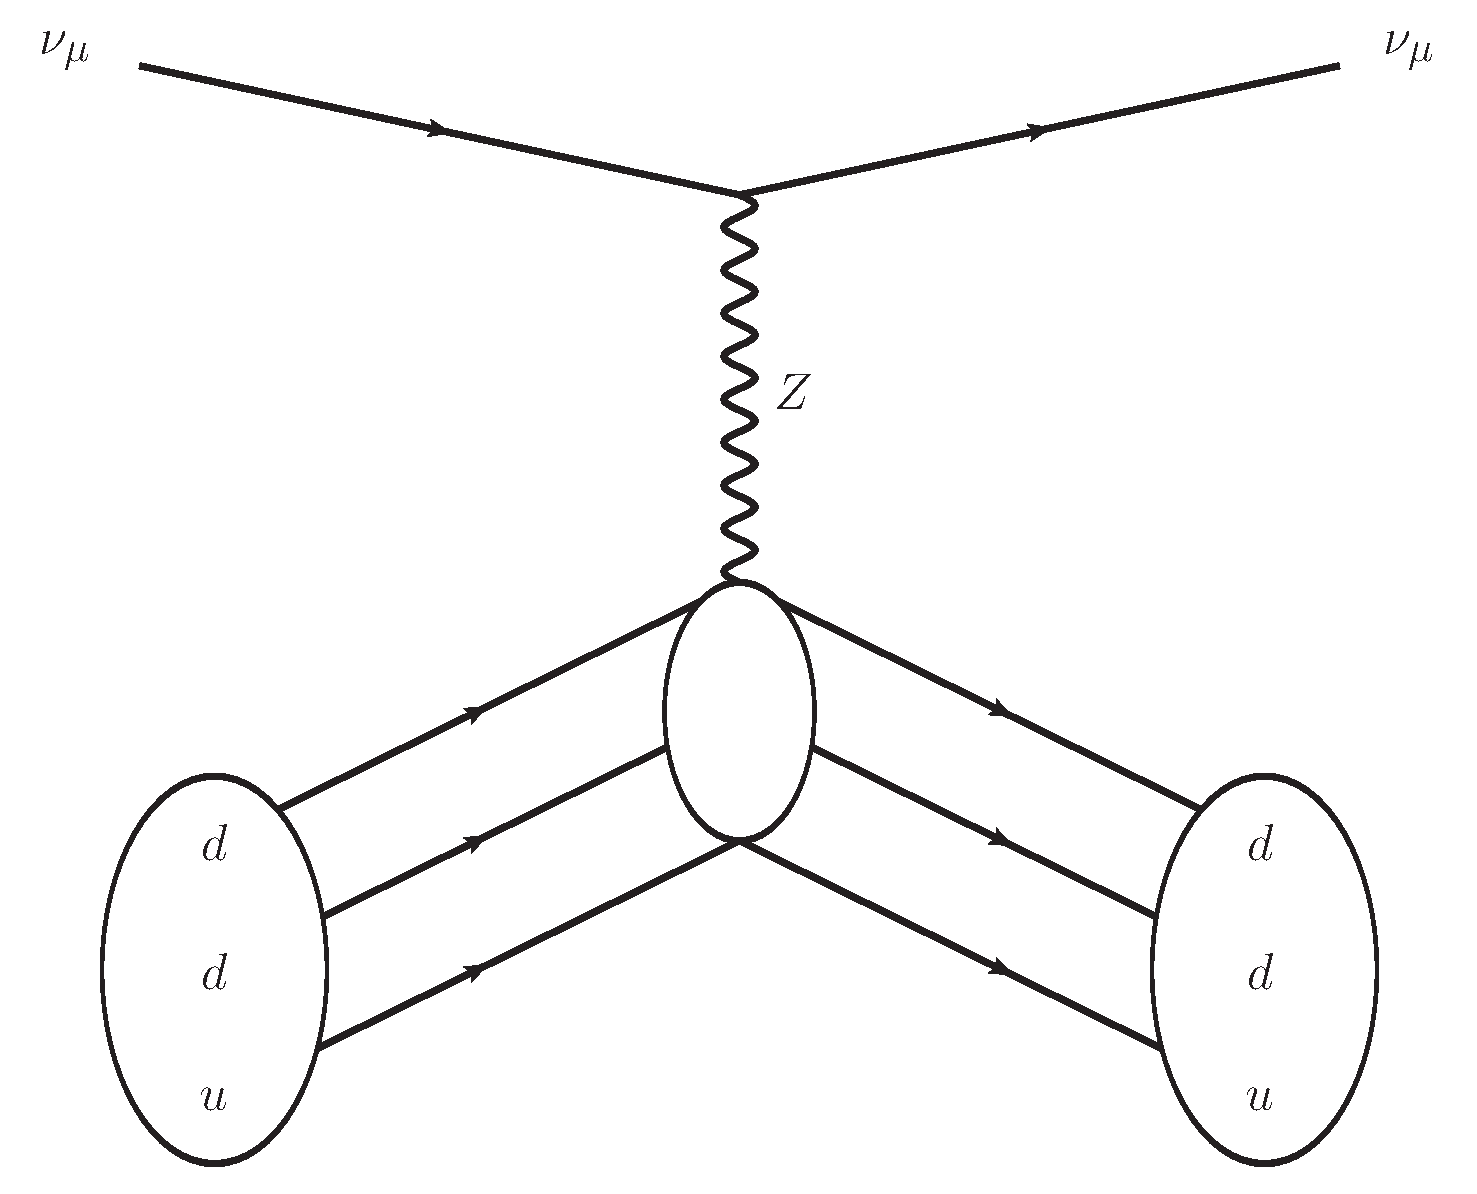
\includegraphics[width=8cm]{images/neutrino_interactions/NCQE_FD.eps} \label{fig:NCQEFD}}
  \caption{Quasi-Elastic (QE) interactions of a $\nu_\mu$ with a nucleon.  The small ellipse represents the neutrino interacting with the nucleon as a whole, rather than with an individual parton.}
  \label{fig:QEFD}
\end{figure}
\newline
\newline
For higher energy neutrinos, there is sufficient energy to promote the target nucleon to an excited state.  A quick after-effect of this promotion is that the excited state decays, resulting in further particle emission.  This interaction topology, which dominates in the 1~GeV to 5~GeV energy range, is known as RESonant pion (RES) production as the neutrino interaction produces $\Delta$ resonance which typically decays to a nucleon and a single pion in the final state.  In the case of $\nu_\mu$ CCRES, the interaction generally takes the following form
\begin{equation}
\nu_\mu N \rightarrow \mu^- N^{*},
\label{eq:CCRES}
\end{equation}
\begin{equation}
N^{*} \rightarrow \pi N',
\end{equation}
where $N, N' = n, p$.  An example diagram of a $\nu_\mu$-CCRES interaction with a $\pi^+$ in the final state is shown in Fig.~\ref{fig:CCRESFD}.
\begin{figure}%
  \centering
  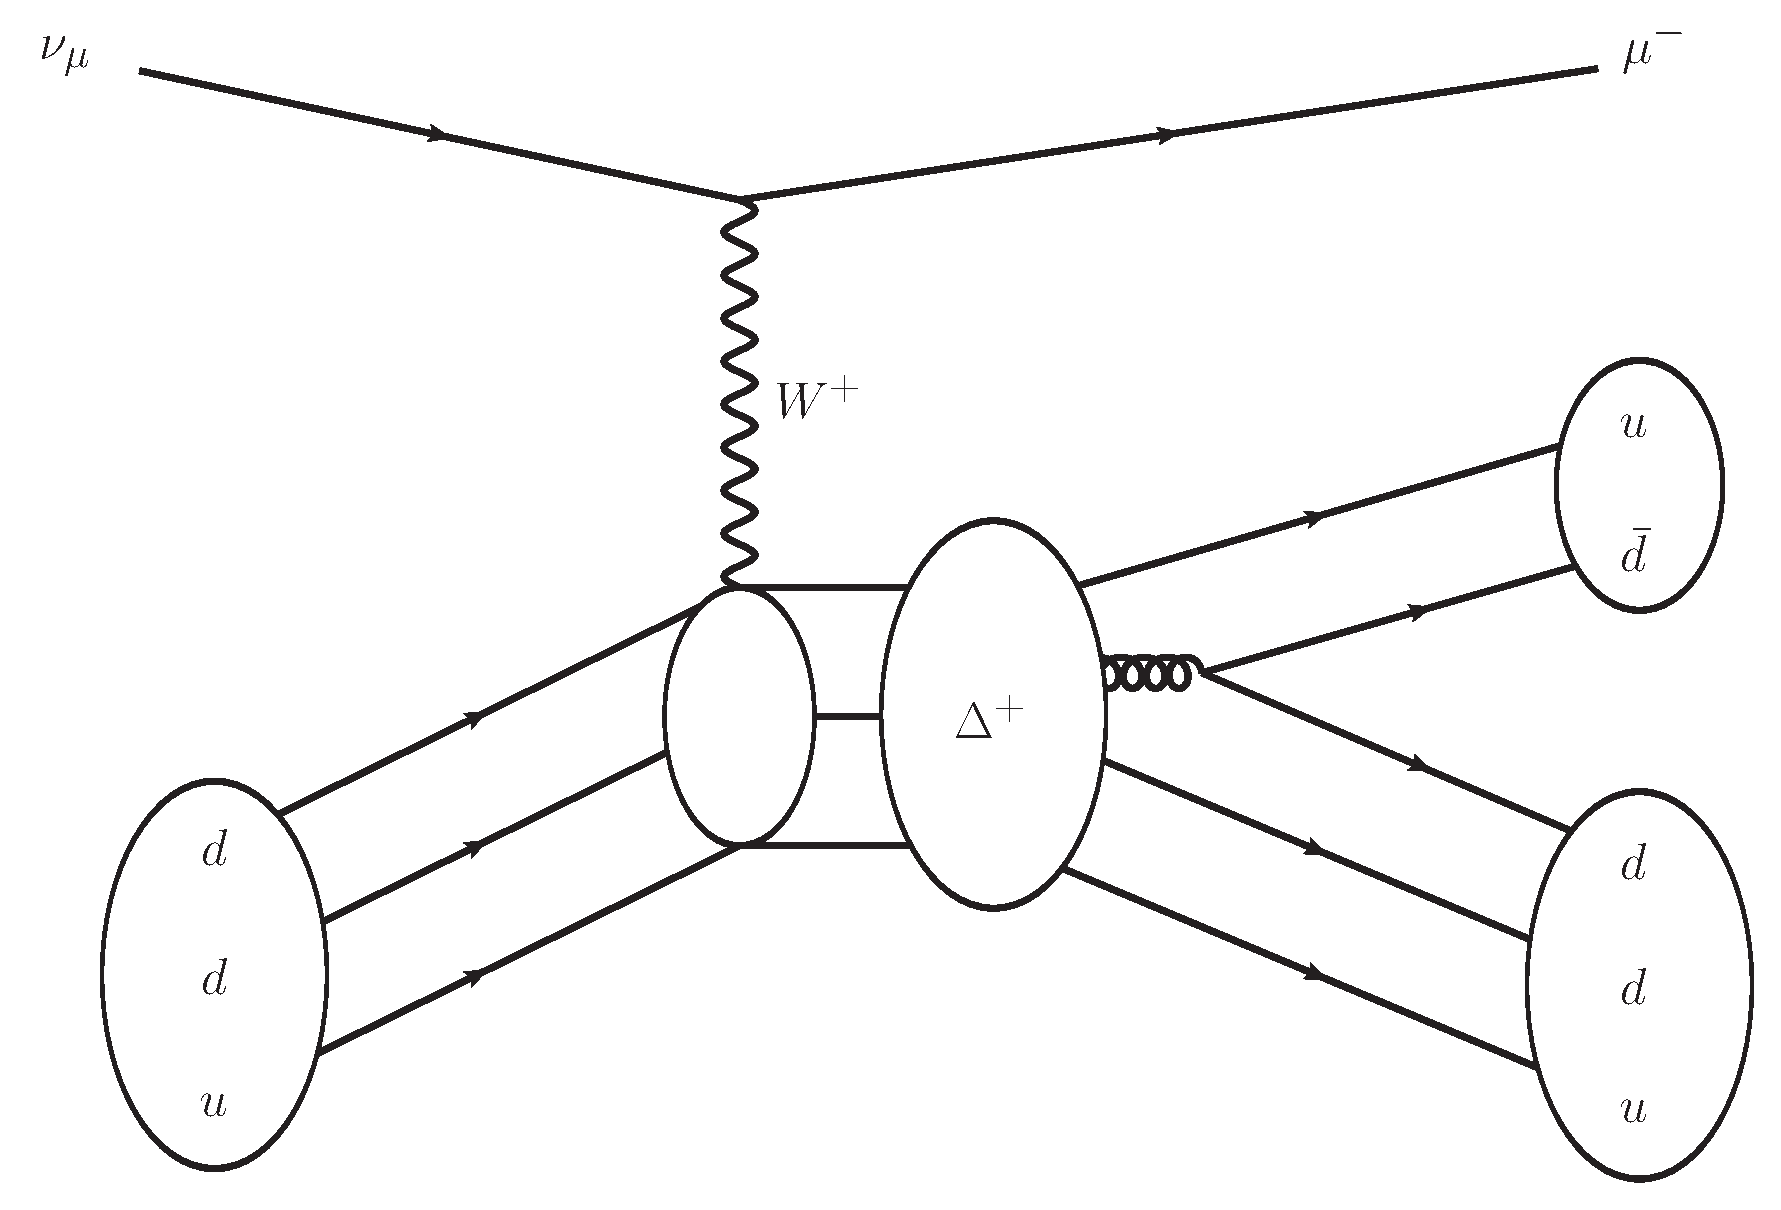
\includegraphics[width=8cm]{images/neutrino_interactions/CCRES_FD.eps}
  \caption{A Charged Current RESonant pion (CCRES) interaction of a $\nu_\mu$ with a neutron.  The $\Delta$ resonance decays to a neutron and a $\pi^+$.}
  \label{fig:CCRESFD}
\end{figure}
\newline
\newline
For neutrinos with energy above the RES-dominant region, the neutrino has enough energy to penetrate the nucleon and scatter off an individual quark.  Because of the nature of the strong force, the scattered quark and the nucleon remnant produce a hadronic shower in the final state.  This process is known as Deep Inelastic Scattering (DIS).  For $\nu_\mu$-CCDIS, the interaction takes the following form
\begin{equation}
\nu_\mu N \rightarrow \mu^- X,
\label{eq:CCDIS}
\end{equation}
where $X$ is the remnant of the nucleus after the interaction occurs.  An example diagram of a $\nu_\mu$-CCDIS interaction is shown in Fig.~\ref{fig:CCDISFG}.
\begin{figure}%
  \centering
  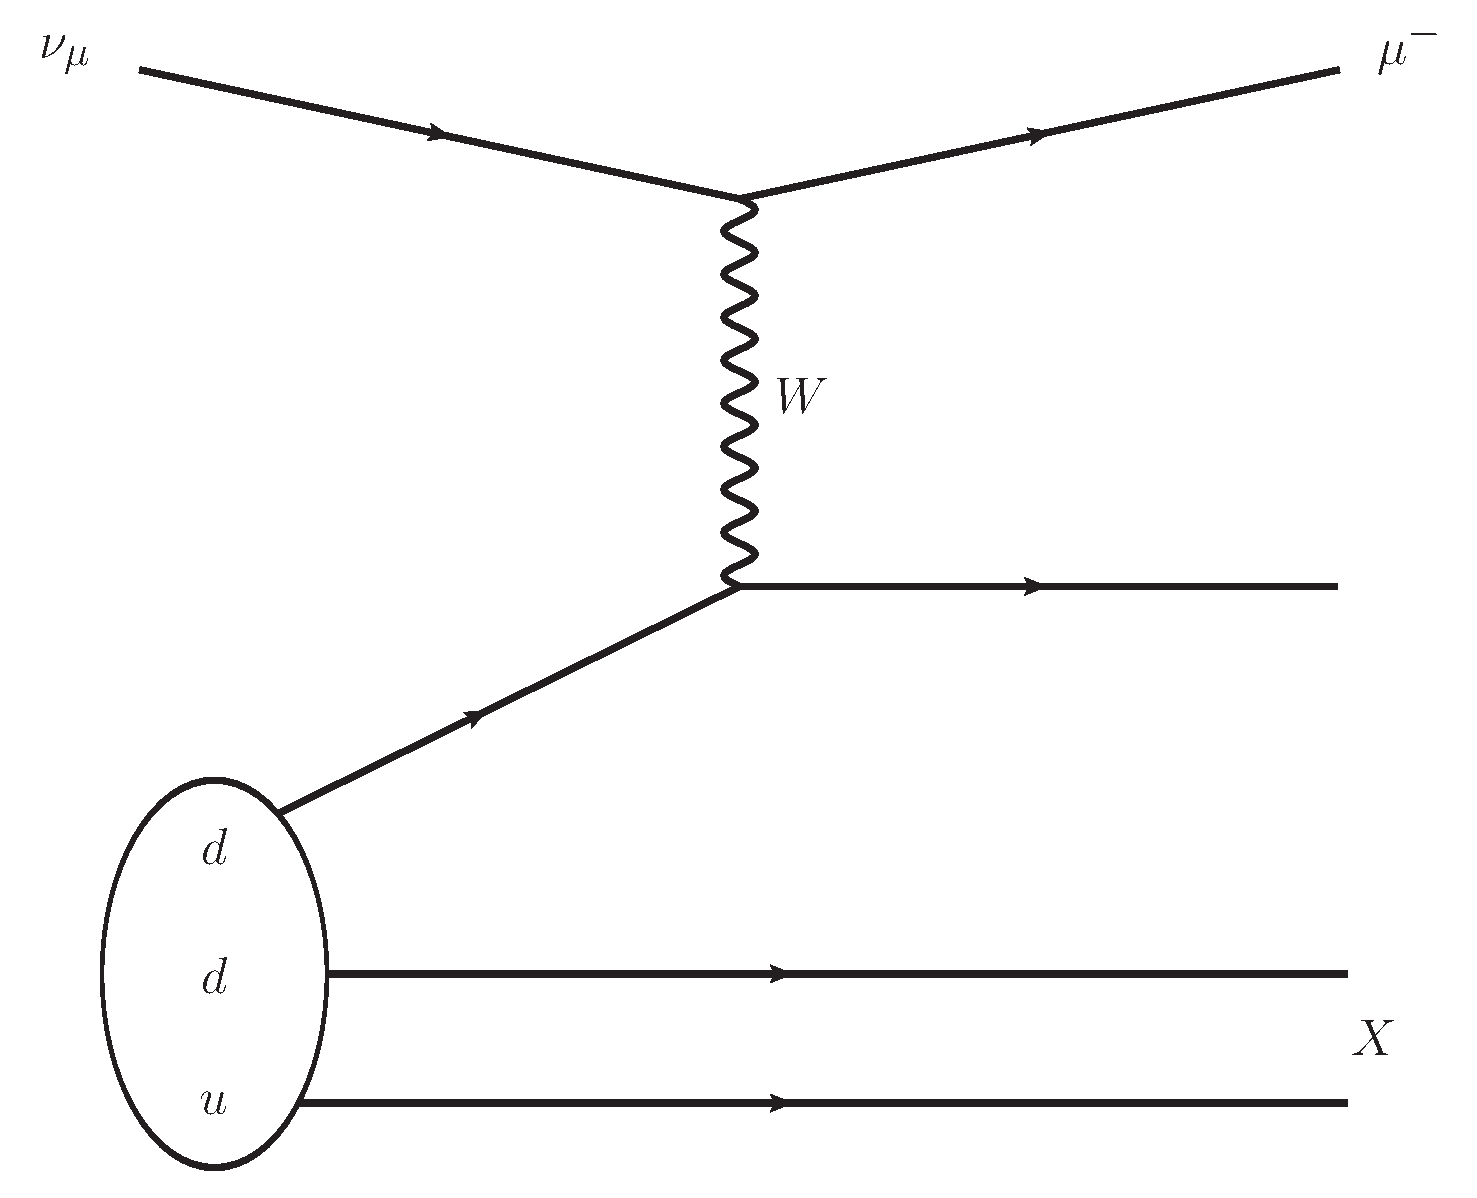
\includegraphics[width=8cm]{images/neutrino_interactions/CCDIS_FD.eps}
  \caption{A Charged Current Deep Inelastic Scattering (CCDIS) interaction of a $\nu_\mu$ with a neutron. $X$ \Yoshi{represents}{was `resembles'} the leftover nuclear remnant.}
  \label{fig:CCDISFG}
\end{figure}
\newline
\newline
While the value of a particular interaction cross-section should depend on the nuclear environment, it is possible to make comparisons of the measured cross-section per nucleon.  Fig.~\ref{fig:CrossSectionMeasurements}\Yoshi{}{Make this figure bigger. Say something about the data points as well as the curves, and how up-to-date it is etc} shows a comparison of $\nu_\mu$ CC cross-section measurements per nucleon from different experiments, all of which sample a different neutrino energy range.  There are large uncertainties for many of the cross-section measurements, particularly for the ones sampling the lower energy ranges.  The T2K beam energy is $\sim$700~MeV, which sits in the region of higher uncertainty.
\begin{figure}[b]%
  \centering
  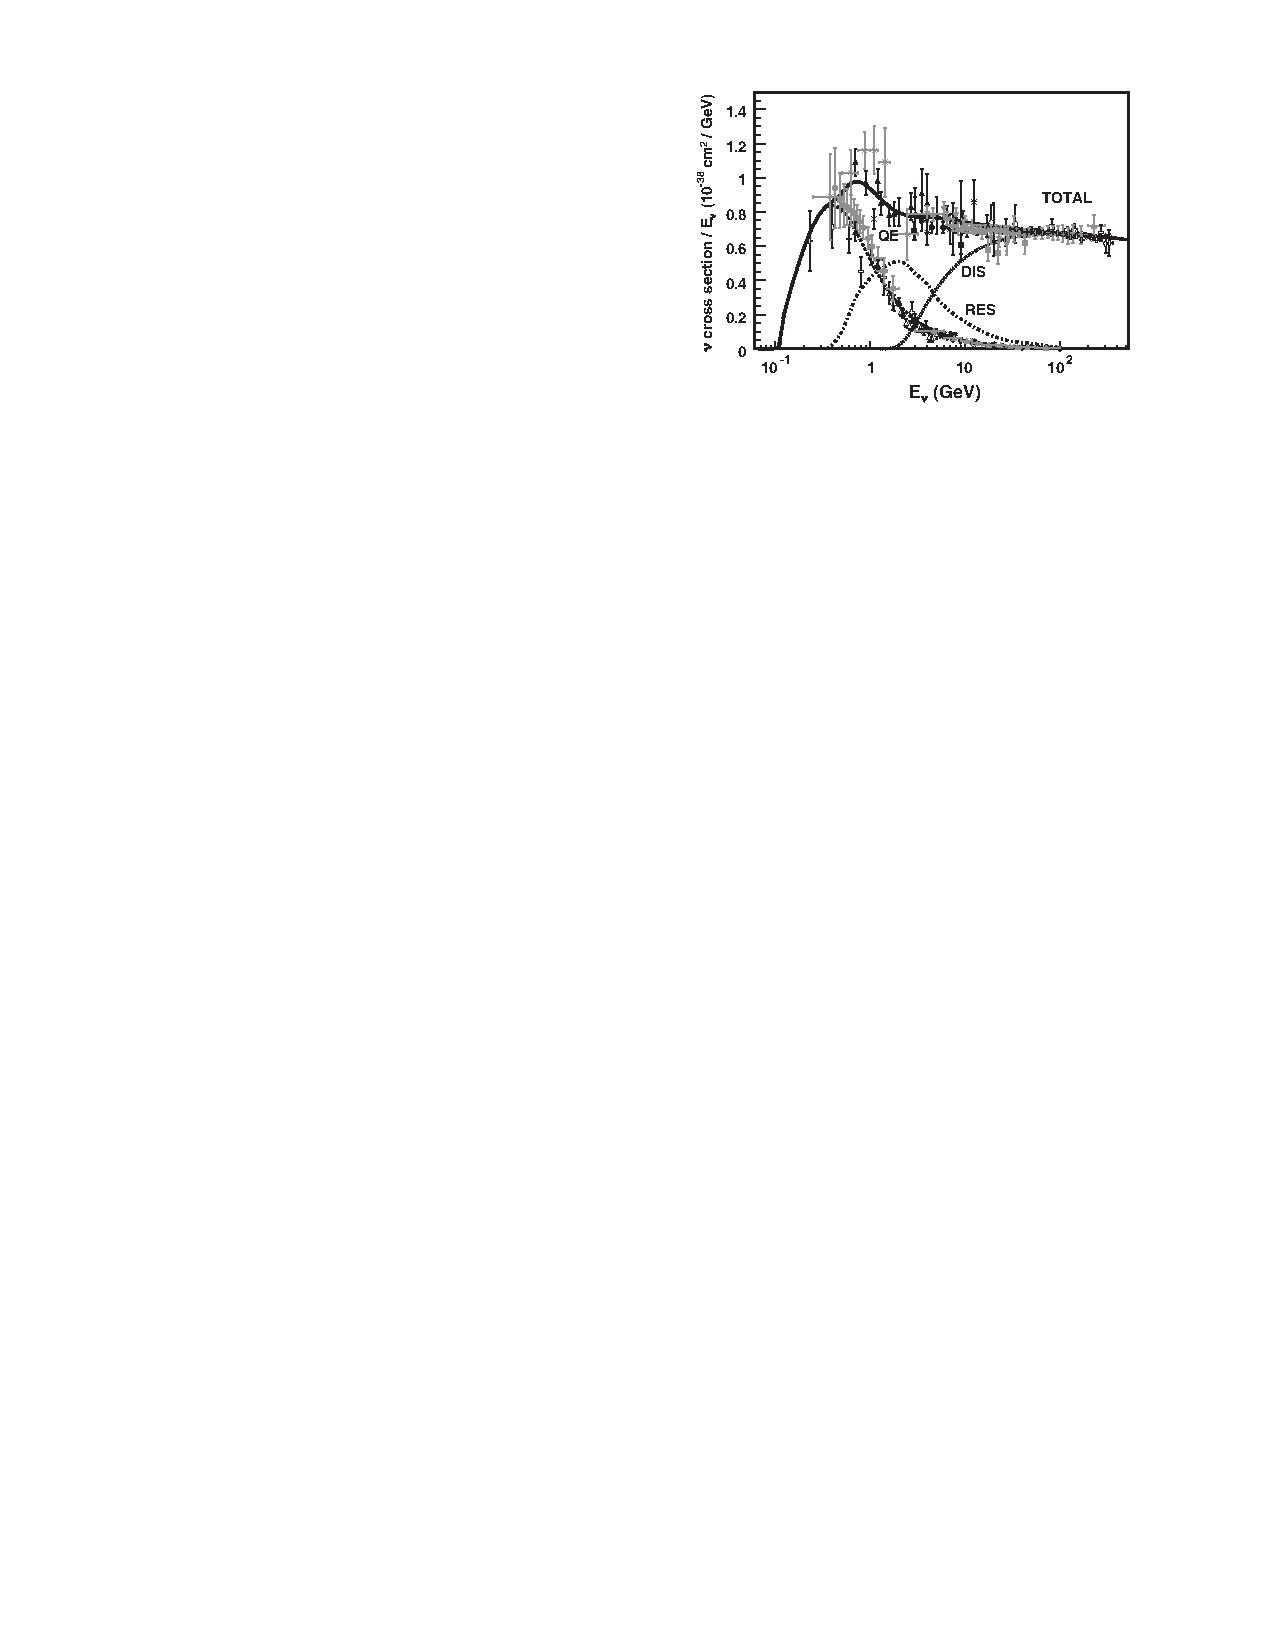
\includegraphics[width=8cm]{images/neutrino_interactions/CrossSectionMeasurements.pdf}
  \caption{$\nu_\mu$ CC cross-section measurements per nucleon for a range of energies, showing the QE, RES and DIS contributions~\cite{RevModPhys.84.1307}.}
  \label{fig:CrossSectionMeasurements}
\end{figure}
\newline
\newline
CCQE interactions are experimentally the most interesting and this is the interaction region where most recent measurements have been focused.  Because of the simplicity of the CCQE topology, the interaction can be treated as a two-body scatter.  So, by applying simple conservation rules, the neutrino energy can be kinematically reconstructed.  In such interactions, the nucleon structure is parameterised using a set of form factors, the most interesting of which is the axial-vector form factor, $F_A(Q^2)$. $F_A(Q^2)$ has been, and still is, assumed to take a dipole form
\begin{equation}
F_A(Q^2) = \frac{F_A(0)}{(1-Q^2/M_A^2)^2}
\label{eq:FAFormFactor},
\end{equation}
where $Q^2$ is the negative of the squared four-momentum transfer of the lepton to the hadron, $F_A(0) = 1.2694\pm0.0028$~\cite{0954-3899-37-7A-075021}, and $M_A$ is known as the axial mass.  Recent measurements of the CCQE cross-section by the MiniBooNE~\cite{PhysRevD.81.092005} and NOMAD~\cite{NOMAD-CCQE} experiments have sparked interest by reporting measured cross-sections which are in tension with one another, the results of which shown in Fig.~\ref{fig:CCQECrossSectionMiniBooNENOMAD}.  
\begin{figure}%
  \centering
  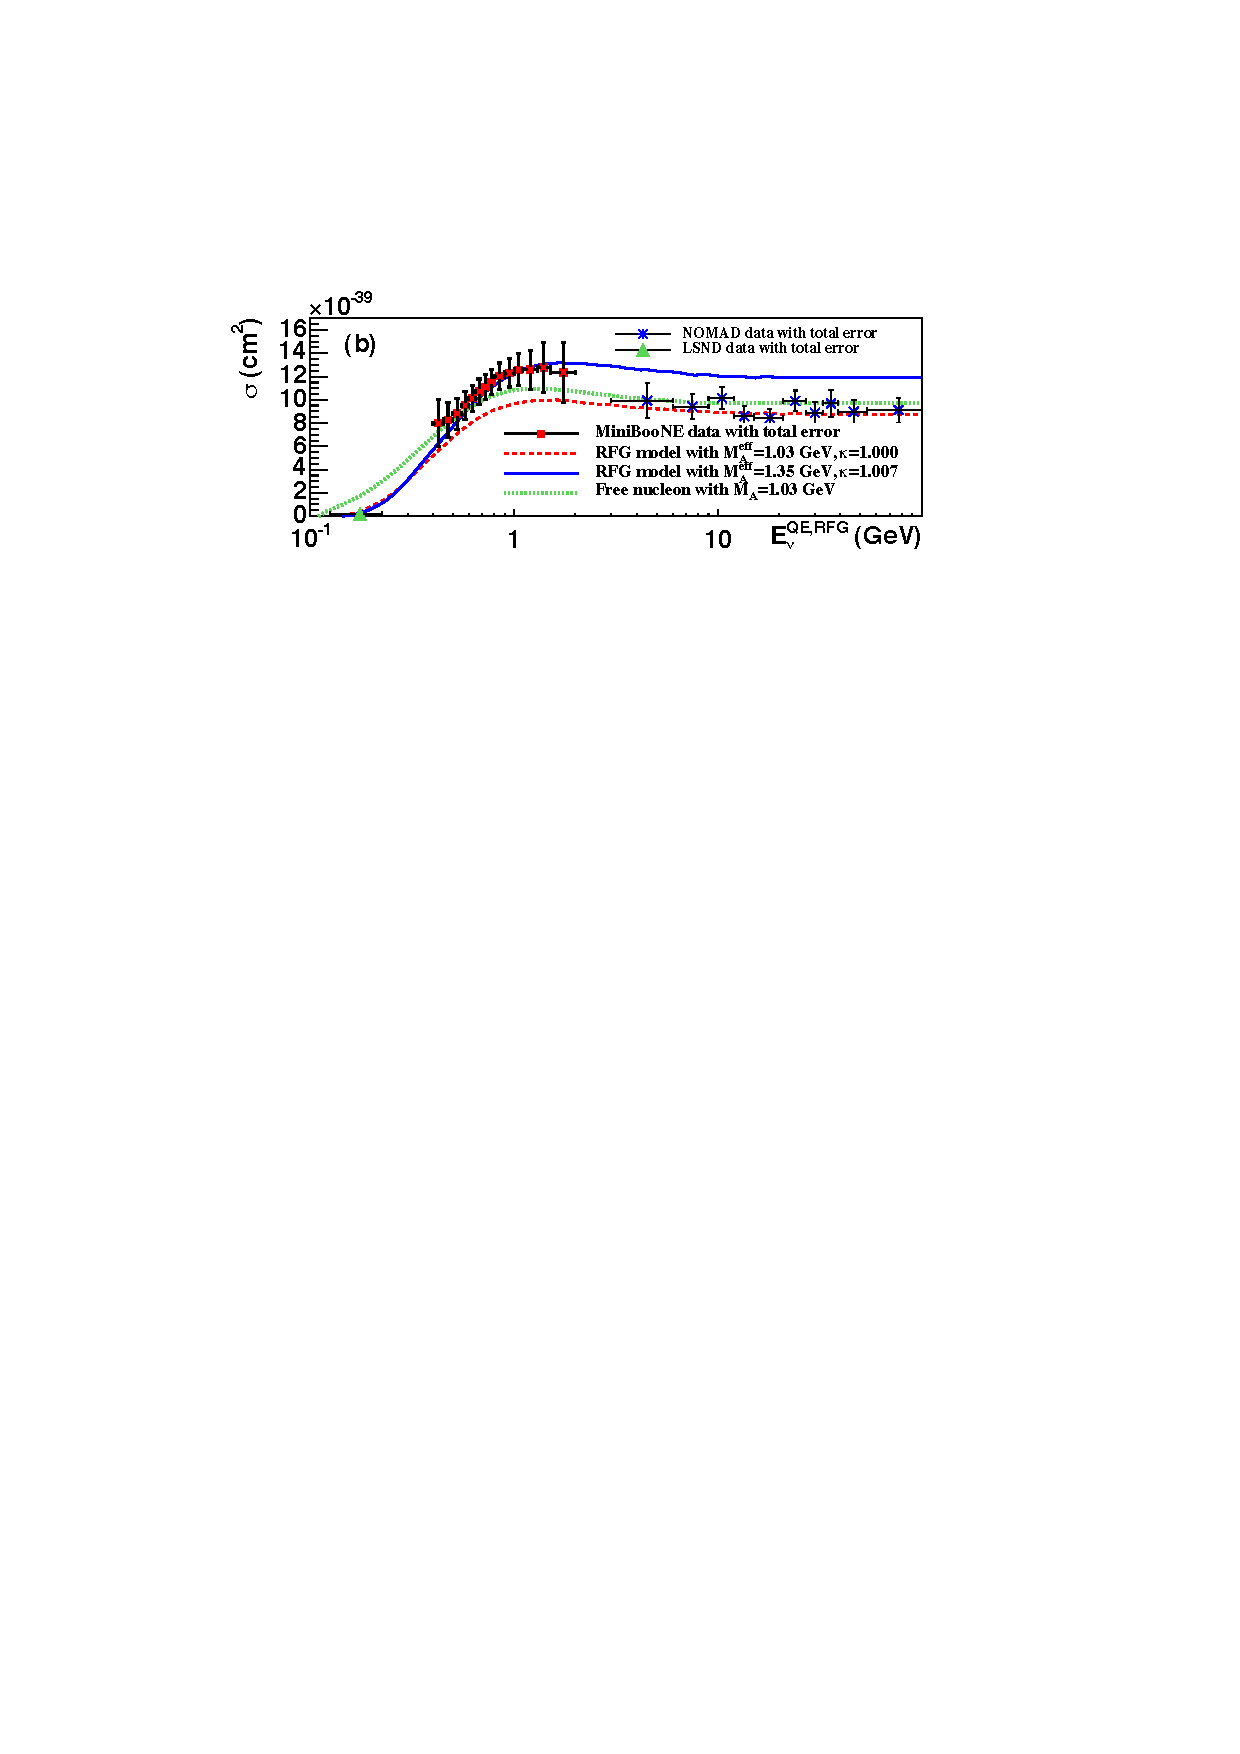
\includegraphics[width=12cm]{images/neutrino_interactions/CCQECrossSectionMiniBooNENOMAD.pdf}
  \caption{The CCQE cross-sections measured by the MiniBooNE and NOMAD experiments.  The solid and dashed lines represent models with different values of $M_A$~\cite{PhysRevD.81.092005}.}
  \label{fig:CCQECrossSectionMiniBooNENOMAD}
\end{figure}
A popular explanation for this discrepancy is a lack of understanding of the nuclear environment.  Because the neutrino is not scattering of a free nucleon, but rather a nucleon in a strongly contained system, experiments actually measure an effective $M_A$.  It is possible that the nuclear effects cause a modification to the effective $M_A$ that the experiments measure.  This possible explanation for the discrepancy has placed a heavier emphasis on nuclear modelling in neutrino interaction experiments. 
\section{Neutrino interactions with heavy nuclei}
\label{sec:NeutrinoInteractionsHeavyNuclei}
As introduced above, consideration of nuclear effects in cross-section measurements is important.  This is especially true for neutrino interactions on heavy target nuclei.  As one can imagine, the presence of a nucleus can dramatically effect the interactions that are observed in a detector.  A popular model for the nucleus is the Relativistic Fermi-Gas (RFG) model~\cite{Smith:1972xh}.  The RFG model treats the nucleus as a collection of non-interacting nucleons sitting in a potential well.  The nucleons are stacked in the potential well according to the Pauli exclusion principle.  This leads to a uniform momentum distribution of the nucleons up to the Fermi momentum $p_F$.  Importantly, the Pauli exclusion principle has a further effect.  Because the final state nucleon is forbidden from occupying a state taken by another nucleon in the potential well, the energy transfer of the neutrino to the nucleon must result in a final state nucleon with a momentum above $p_F$, resulting in a reduction of the cross-section.
\newline
\newline
The RFG can only model the effect of the nucleus on the initial neutrino interaction which creates the final states.  However, these final states are created within the nucleus and so additional interactions of the final states with the nucleus can occur.  The Final-State Interactions (FSI) can significantly alter the momentum and direction of the final-state particles.  As the final-state particles are used to infer neutrino properties, the FSI effects can alter the interpretation of the reconstructed events.  In simulation, variations of the cascade model are typically used.  This involves pushing the final-state particles through the nucleus in discreet steps and, at each step, probabilistically updating the particle properties.  If at any point a final-state particles knocks out another nucleon, the additional nucleon is also pushed through the nucleus in parallel.  The discreet stepping occurs until all relevant particles have escaped the nucleus.
\newline
\newline
To test such cross-section models, including nuclear effects, it is necessary to compare prediction with collected data.  However, collected cross-section data for heavy nuclei is relatively sparse.  In the case of lead, only two experiments have performed cross-section measurements.  The first measurement was performed by the CHORUS~\cite{CHORUS_XSEC} experiment.  The CHORUS detector, exposed to the CERN SPS beam with a wide-band $\nu_\mu$ beam of 27~GeV average energy, measured a cross-section for lead, iron, marble and polyethylene.  However, because the absolute flux was not measured in the experiment, all of the cross-section measurements were normalised to a common constant.  Their results are summarised in Fig.~\ref{fig:CHORUSXSec}\Yoshi{}{``data/prediction'' is confusing because it looks like the ratio of the two. Say which experiment is, and when the data was taken, in the caption, not just the body text}.
\begin{figure}%
  \centering
  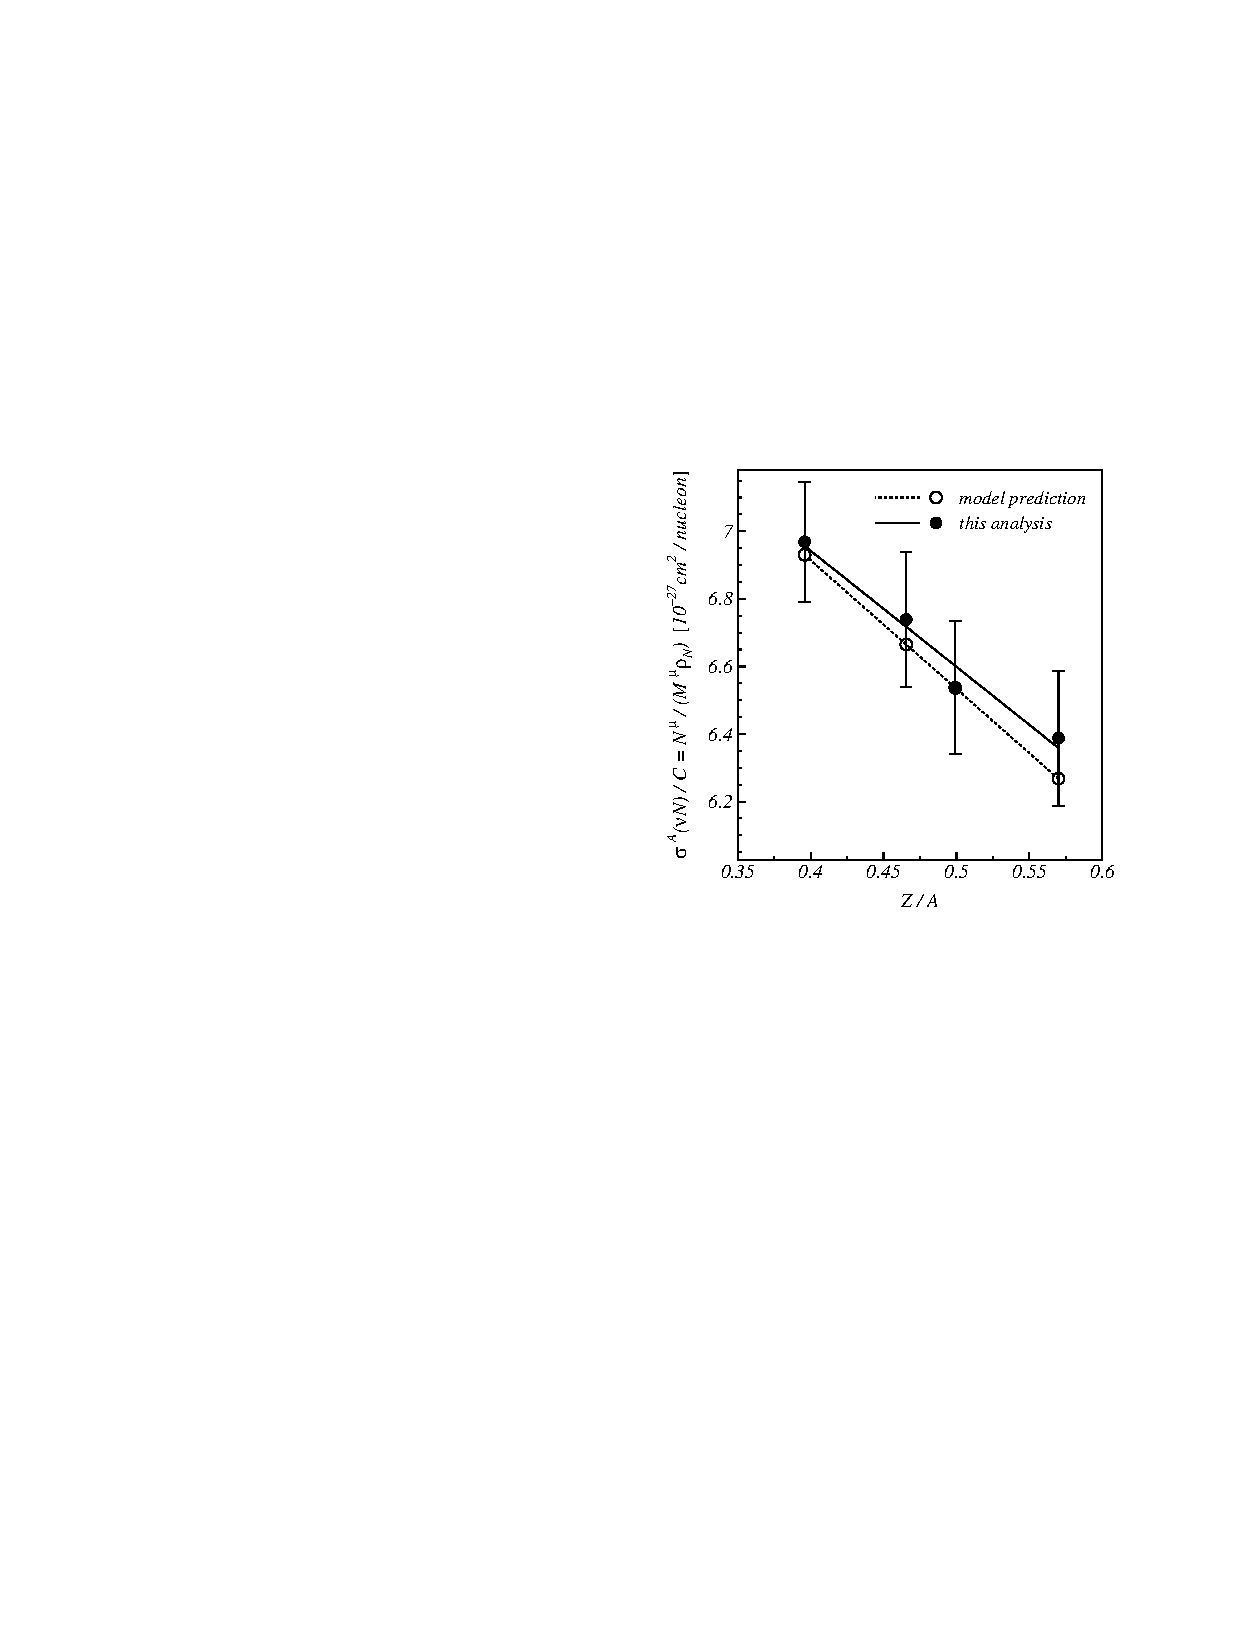
\includegraphics[width=8cm]{images/neutrino_interactions/CHORUS_XSec.pdf}
  \caption{Measured values of the $\nu_\mu$ CC relative cross-section for several elements.  The black and white points are the collected data and prediction respectively.  The solid and dashed lines are the linear best fit lines to the data and prediction respectively.  Going from left to right, the points represent data/prediction for lead, iron marble and polyethylene.}
  \label{fig:CHORUSXSec}
\end{figure}
The second measurement was made by the MINER$\nu$A experiment~\cite{PhysRevLett.112.231801}, which used the Fermilab NuMI beam with a 8~GeV average energy, to measure the relative $\nu_\mu$ CC cross-section on lead to that of plastic scintillator as a function of neutrino energy.  Their results, shown in Fig.~\ref{fig:MINERvAXSec}, largely agreed with the prediction.
\begin{figure}%
  \centering
  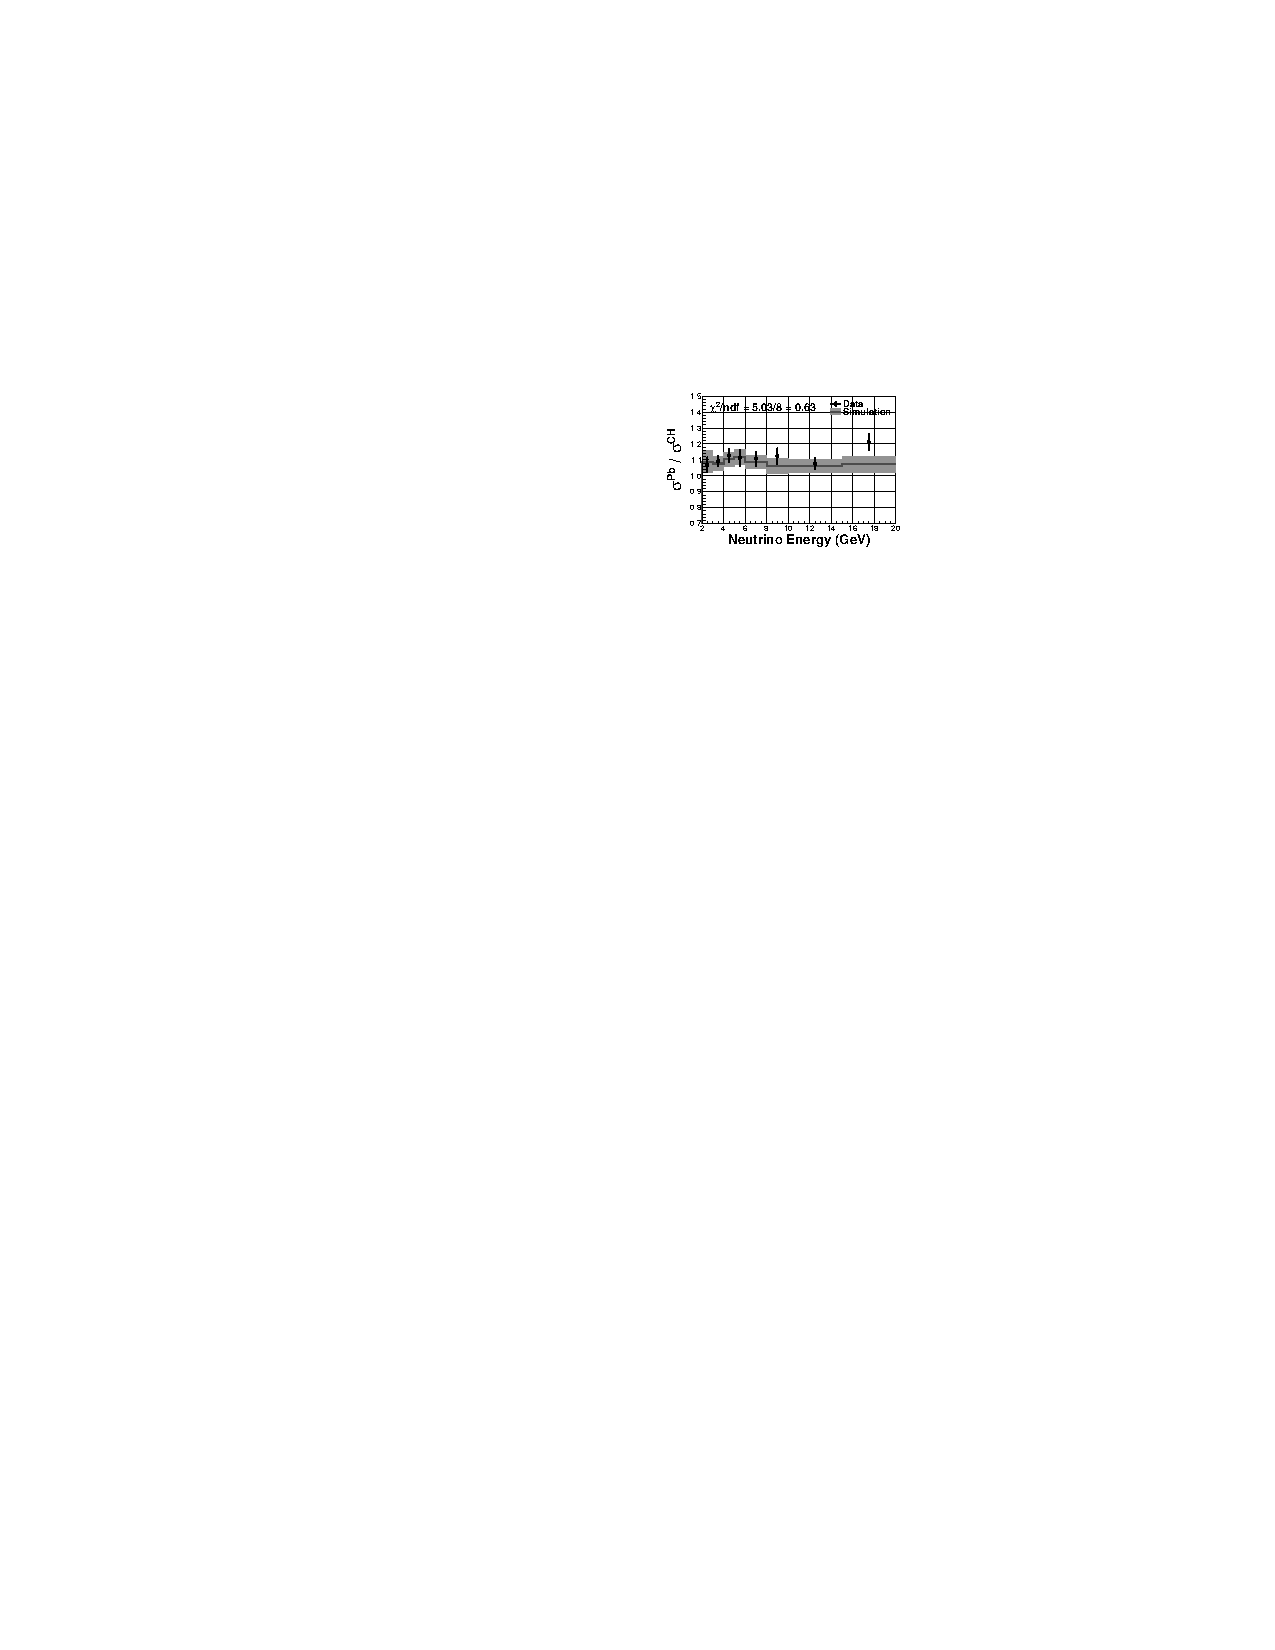
\includegraphics[width=8cm]{images/neutrino_interactions/MINERvA_XSec.pdf}
  \caption{Ratio of the measured $\nu_\mu$ CC inclusive cross-section on lead to plastic scintillator as a function of neutrino energy.  The error bars on the simulation (data) are statistical (systematic) uncertainties~\cite{PhysRevLett.112.231801}.\Yoshi{}{WHAT EXPERIMENT IS THIS? Your captions are generally lacking---they need to stand on their own, without the need for the reader to find the corresponding body text to figure out what a plot is about.}}
  \label{fig:MINERvAXSec}
\end{figure}
\newline
\newline
As neutrino oscillation physics enters the precision era\Yoshi{}{We entered the precision era quite a while ago---see KamLAND's mixing angle error!}, it is becoming increasingly important that our understanding of neutrino cross-sections is improved.  To achieve this goal, more cross-section measurements across a range of nuclear targets are needed.  This thesis presents a measurement of the $\nu_\mu$ CC inclusive cross-section on lead using the electromagnetic calorimeters contained in the near detector of the T2K experiment.  










  %\chapter{The T2K Experiment}
\label{chap:T2KExperiment}
\begin{figure}
  \centering
  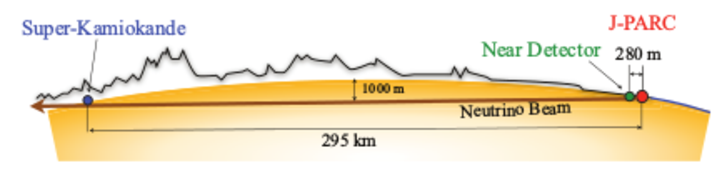
\includegraphics[width=10cm]{images/t2k/t2k_schematic.pdf}
  \caption{Schematic of the T2K experiment showing the near and far sites, separated by the 295~km baseline.}
  \label{fig:T2KSchematic}
\end{figure}

The Tokai-to-Kamioka (T2K) experiment~\cite{Abe2011106} is a long baseline neutrino oscillation experiment located in two sites across Japan and is designed to study the parameters governing the PMNS matrix.  The first site is the J-PARC facility in Tokai-mura on Japan's east cost which houses a 30 GeV proton accelerator complex that is used to generate a highly pure $\nu_\mu$ beam.  J-PARC also contains a suite of detectors designed to measure the neutrino beam's unoscillated characteristics.  Super-Kamiokande (SK) is located 295 km (see Fig.~\ref{fig:T2KSchematic}) and measures the contents of the neutrino beam post-oscillation.
\newline
T2K was the first experiment to observe the $\nu_\mu\rightarrow\nu_e$ appearance channel~\cite{PhysRevLett.112.061802} which excluded $\theta_{13} = 0$ at 7.3$\textrm{\sigma}$ significance.  By comparing this result with precise $\theta_{13}$ measurements from reactor experiments, $\textrm{\delta}_{\textrm{CP}}$ regions can be excluded at 90$\%$ confidence level (see Fig.~\ref{fig:NueAppearanceContour}).  T2K's precision analysis of the $\nu_\mu$ disappearance channel provide world leading measurements of $\textrm{\theta}_{23}$ and $\Delta m^2_{23}$.  Independently of the oscillation analyses performed by the experiment, T2K's near detectors, ND280 and INGRID, are used to measure a range of neutrino cross-sections~\cite{PhysRevLett.113.241803, PhysRevD.87.092003}.  While this is not the primary aim of T2K, such measurements are still extremely important as T2K systematic uncertainties can be constrained with additional cross-section knowledge as well as helping to understand the general neutrino interaction picture.
\begin{figure}
  \centering
  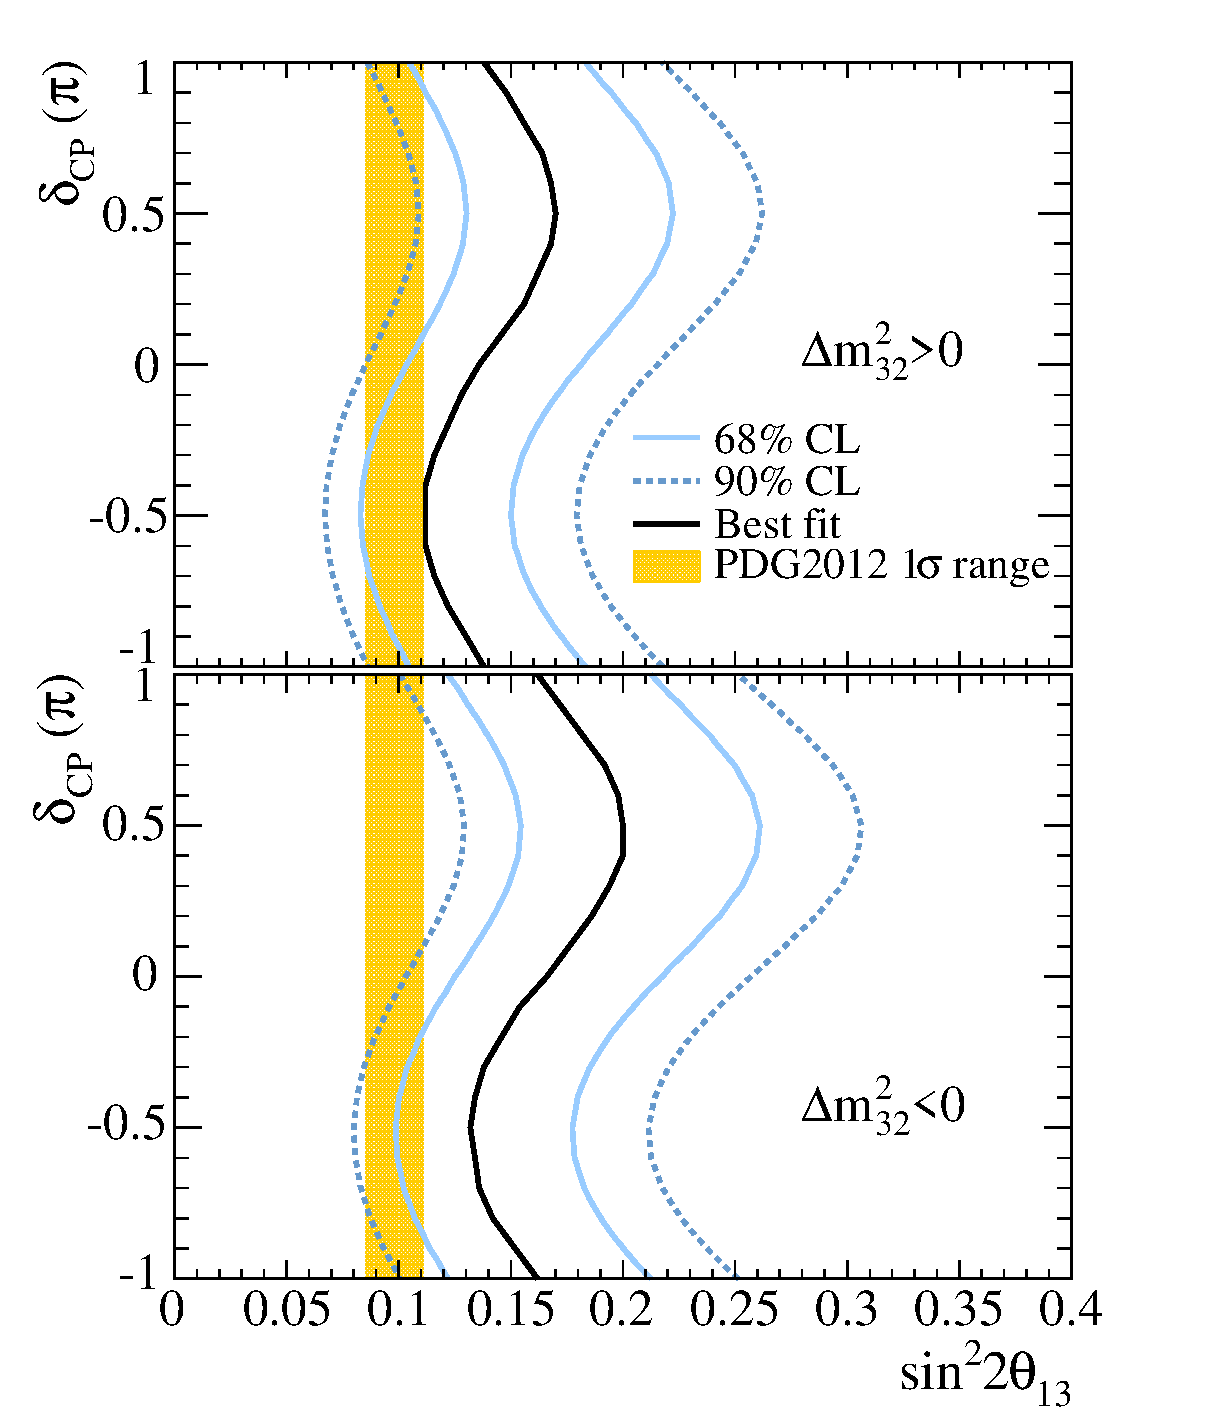
\includegraphics[width=7.5cm]{images/t2k/nue_appearance_Theta13Delta_contour.eps}
  \caption{The 68$\%$ and 90$\%$ confidence level allowed regions for $\sin^22\theta_{13}$ as a function of $\textrm{\delta}_{\textrm{CP}}$ for normal hierarchy (top) and inverted hierarchy (bottom)  The solid line represents the best fit $\sin^22\theta_{13}$ for a given $\textrm{\delta}_{\textrm{CP}}$.  The shaded region shows the average $\theta_{13}$ provided by the reactor constraint~\cite{PhysRevLett.112.061802}.}
  \label{fig:NueAppearanceContour}
\end{figure}


\section{T2K beam}
\label{sec:T2KBeam}
The T2K neutrino beam is generated by J-PARC's accelerator complex which produces a 30 GeV proton beam which is fired at a fixed graphite target.  The final-state particles of interactions with the target are predominately charged pions which decay to produce the neutrino beam.  Surrounding and behind the graphite target are a set of magnetic horns which focus the pions into a beam, resulting in a focused neutrino beam after the hadrons have decayed.

\subsection{Accelerator complex}
\label{subsec:AcceleratorComplex}
The J-PARC accelerator complex consists of three sections: the LINnear ACcelerator (LINAC), the Rapid-Cycling Synchrotron (RCS) and the Main Ring synchrotron (MR).  Production of the proton beam starts at the LINAC where H$^-$ anions are accelerated to 181 MeV which are subsequently converted to H$^+$ ions via charge-stripping foils at the RCS injection point.  With a 25 Hz cycle, the ions are further accelerated by the RCS to 3 GeV with two bunches per cycle.  Roughly 5$\%$ of the proton bunches are fed into the MR where the final acceleration to 30 GeV occurs in bunches of eight.  Extraction of the bunches occurs at two points for different experiments.  For T2K, all eight bunches are extracted in a single turn by five kicker magnets and aimed down the neutrino beamline to the graphite target.  The extraction of all eight bunches forms a single beam spill with a width of 5 $\mu$sec.  The tight structure of the beam spills is vital for background discrimination in the downstream detectors.

\subsection{Neutrino beamline}
\label{subsec:NeutrinoBeamline}

\begin{figure}
  \centering
  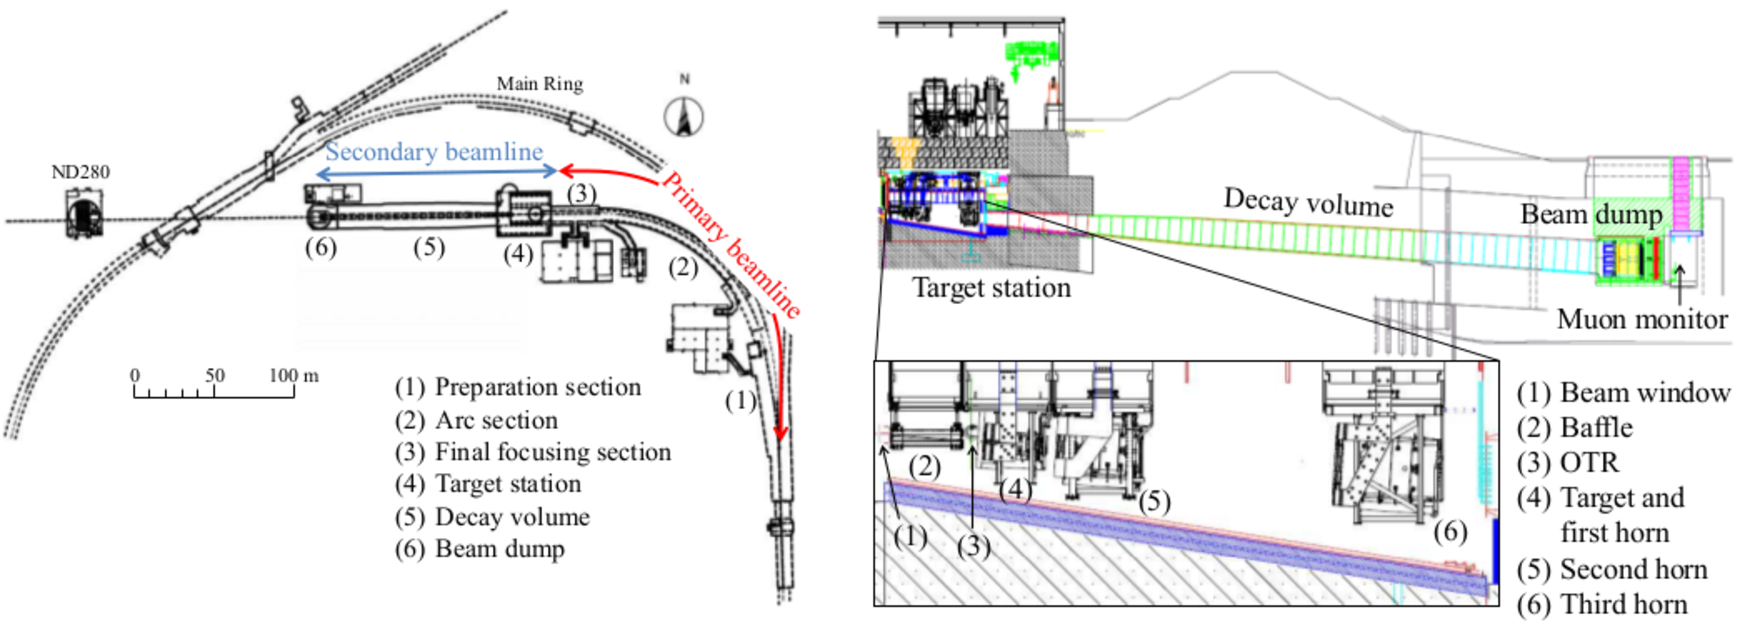
\includegraphics[width=15cm]{images/t2k/neutrino_beamline.pdf}
  \caption{A schematic of the T2K neutrino beamline (left) and a side view of the secondary beamline (right)~\cite{Abe2011106}.}
  \label{fig:NeutrinoBeamline}
\end{figure}

The neutrino beamline (NU) is split into a primary and secondary beamline, a schematic of which is shown in Fig.~\ref{fig:NeutrinoBeamline}.  The primary beamline consists of a preparation section, an arc section and a focusing section.  The preparation section uses 11 normal conducting magnets to tune the proton beam for entry into the arc section where the proton beam is bent to its intended direction.  As will be discussed in more detail in section~\ref{subsec:OffAxisBeam}, the axis of the beam is 2.5$^\circ$ away from SK.  The final focusing sections then guides the proton beam into the secondary beamline and the graphite target.
\newline
\newline
Sound performance of the proton beam is vital for stability of the T2K neutrino beam.  To ensure such performance, the primary beamline is equipped with a suite of monitors to measure the position, profile, loss and intensity of the proton beam.  The beam position is measured by 21 ElectroStatic Monitors (ESMs) which consists of four cylindrical electrodes surrounding the beam.  The asymmetry of the beam is measured by the induced current in the electrodes which is used to infer the position in a non-destructive manner.  Segmented Secondary Emission Monitors (SSEMs) are used to measure the beam loss.  Each SSEM has an anode foil sandwiched between two titanium foil strips.  Protons interact with the strips causing an emission of electrons which electrically drift inducing a current in the strips.  The charge distribution is used to reconstruct the profile.  The Beam Loss Monitors (BLMs) are Ar-CO$_2$ filled wire proportional counters and are used to quantify the beam loss.  The intensity of the beam is measured by five Current Transformers (CTs) which consist of a 50-turn toroidal coil around a ferromagnetic coil.  Passage of the beam induces a current in the coil which is used to infer the number of protons in the spill.  The final CT (CT5) is positioned at the end of the focusing section of the primary beamline and is used to count the number of protons incident on the graphite target.  The accumulated number of protons on target (POT) is used as a metric for the data collected by T2K.  The total POT accumulated so far by T2K is shown in Fig.~\ref{fig:POTHistory}.
\begin{figure}
  \centering
  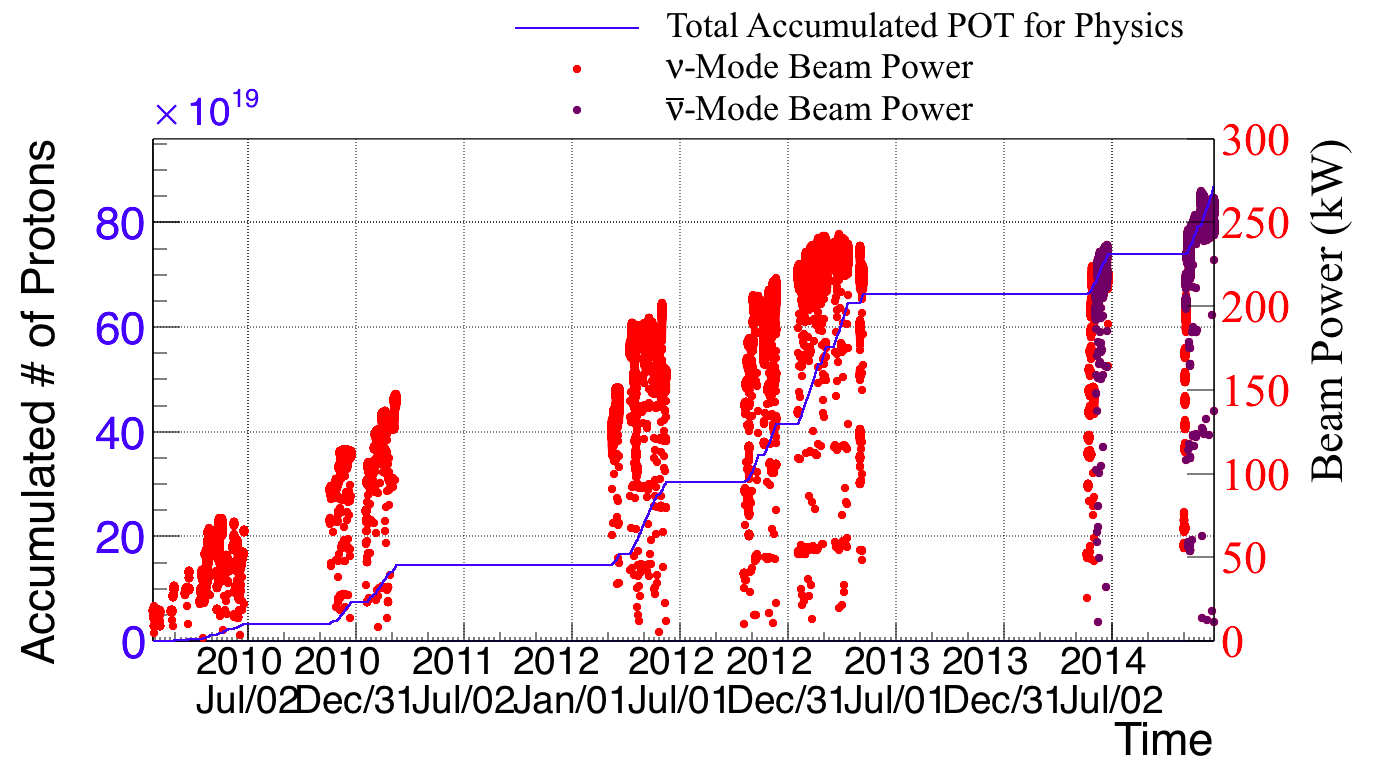
\includegraphics[width=15cm]{images/t2k/pot_history.png}
  \caption{The POT recorded by CT5 as a function of time (blue line) and the recorded beam power in $\nu$ running mode (red dots) and $\bar{\nu}$ running mode (purple dots).}
  \label{fig:POTHistory}
\end{figure}
\newline
The secondary beamline consists of the graphite target, a set of magnetic focusing horns, a decay pipe and a beam dump.  A schematic for the secondary beamline is shown in Fig.~\ref{fig:NeutrinoBeamline}.  The graphite target is a 2.6 cm diameter and 91.4 cm long rod which is surrounded by a 2 mm thick graphite tube and a 0.3 mm titanium case.  The proton-graphite interactions produce charged pions and kaons which are focused by three magnetic horns, one of which surrounds the target.  The magnetic horns consist of two coaxial conductors which generate a magnetic field with a strength inversely proportional to the distance from the beam axis.  The current direction in the magnetic horns causes the induced field to focus or deflect particles depending on their charge sign.  This simple control allows T2K to operate in $\nu$ or $\bar{\nu}$ beam mode.  The focused mesons then travel down a decay pipe filled with Helium to reduce pion absorption.  It is here that the mesons decay to produce the neutrinos which form the T2K beam.  To stop measurement contamination, other decay products must be stopped before reaching the downstream detectors.  So, a 75 ton graphite beam dump is positioned at the end of the decay volume.  The beam dump stops almost all non-wanted decay products, with only 5 GeV or above muons successfully propagating through.  As the muons are generally simultaneously produced with the beam neutrinos, measurements of the muons can be used to monitor the direction of the neutrino beam.  To do this, a MUon MONitor (MUMON) is installed at the downstream end of the beam dump.

\subsection{Off-axis beam}
\label{subsec:OffAxisBeam}
The kinematics of the pion decays dictate the energy spectrum shape of the neutrinos.  Specifically, the peak width of the neutrino energy narrows and shifts as an observer moves off-axis from the pions trajectory.  As the pions are the neutrino parents in the T2K beam, the same effect can be seen by moving off-axis from the neutrino beam.  This effect is illustrated in Fig.~\ref{fig:OAEffectFlux}.  By positioning T2K's baseline detectors at 2.5$^\circ$ off-axis, it is possible to align the neutrino beam's peak energy with the first oscillation maximum for the $\nu_\mu$ disappearance channel.  Separately, an off-axis configuration reduces the beam's unwanted high energy tail, improving sensitivity to $\nu_e$ appearance and $\nu_\mu$ disappearance.
\begin{figure}
  \centering
  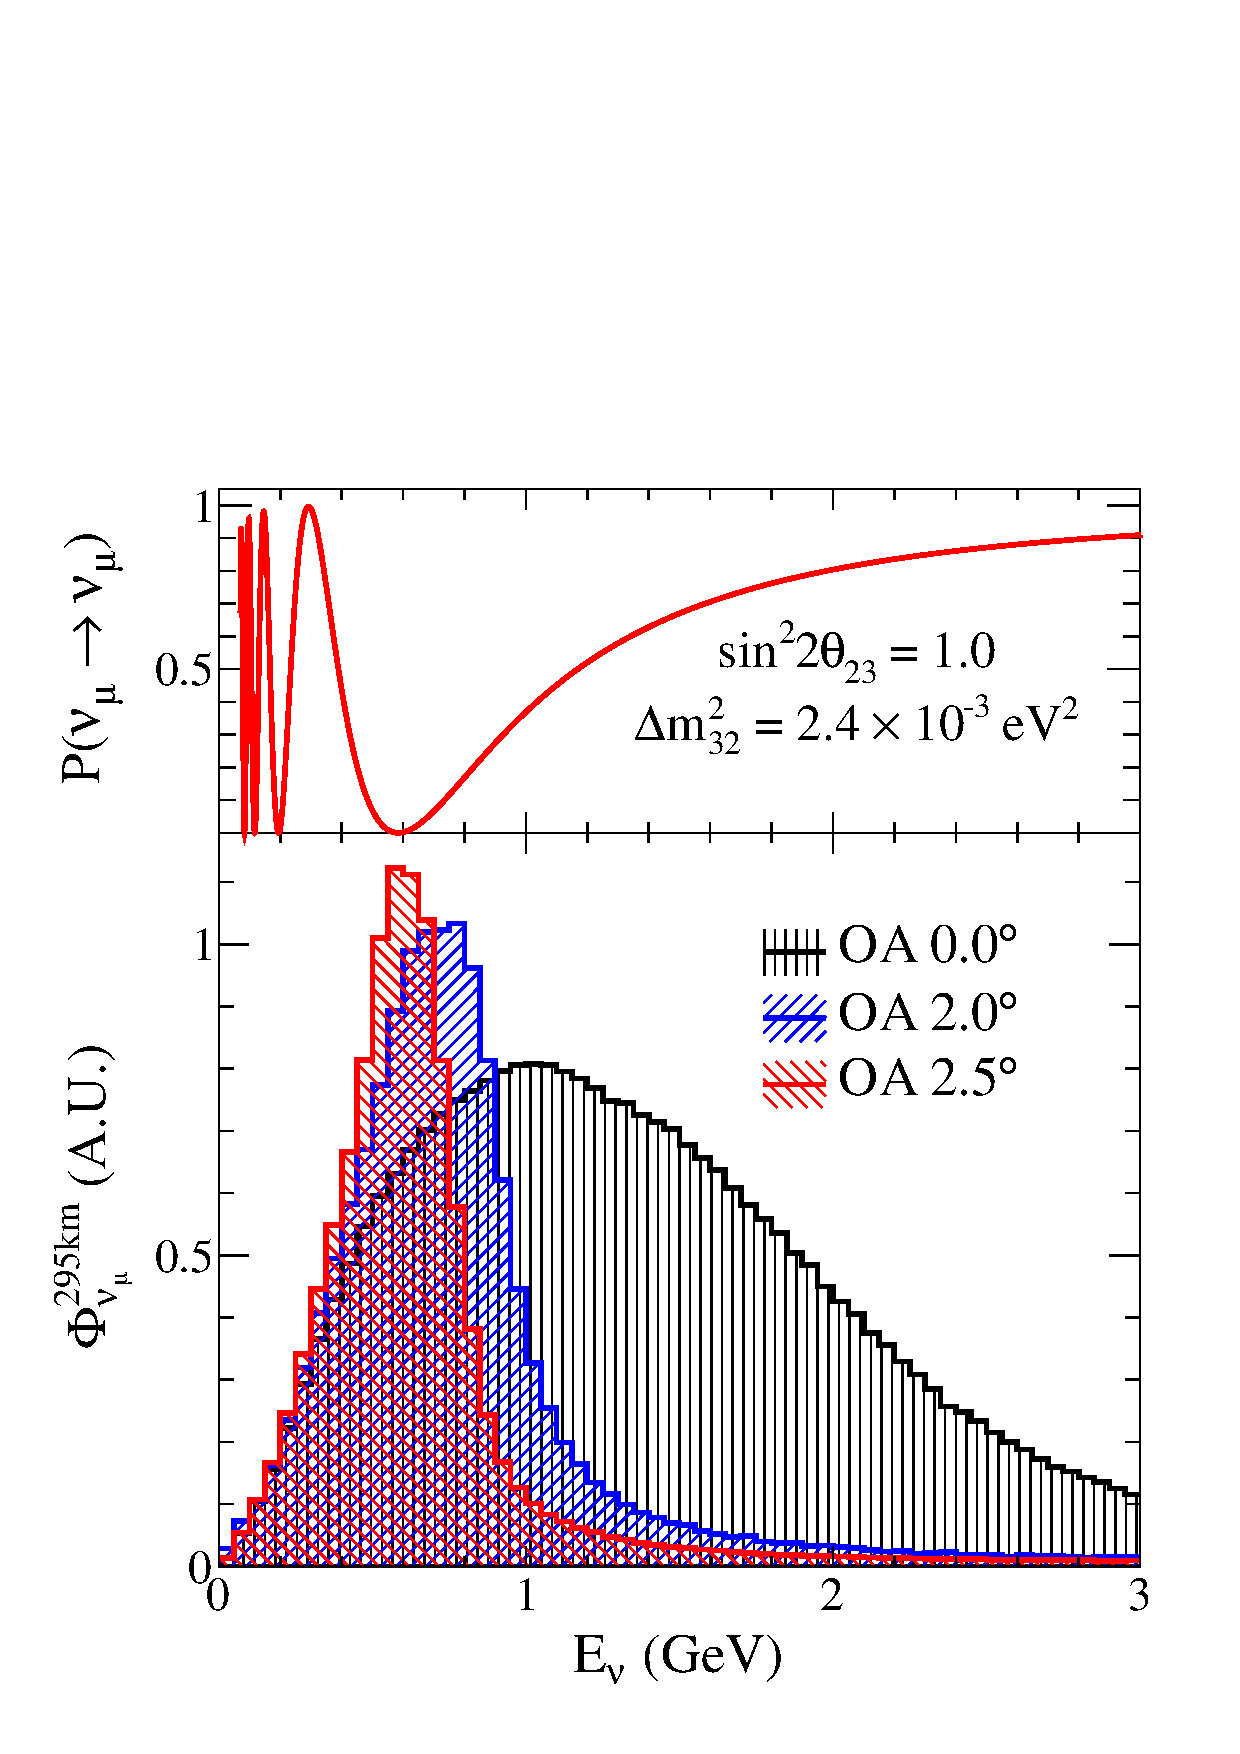
\includegraphics[width=7cm]{images/t2k/oaeffect_flux.pdf}
  \caption{Muon neutrino survival probability at 295~km (top) and neutrino fluxes for different off-axis angles (bottom)~\cite{PhysRevD.87.012001}.  The peak neutrino lowers and the energy distribution narrows as the off-axis angle increases.}
  \label{fig:OAEffectFlux}
\end{figure}



\section{Near detector complex}
\label{sec:NearDetectorComplex}
Located 280~m downstream of the beam target is the near detector complex which houses a pair of detectors which measure the unoscillated characteristics of the beam.  The two detectors, named INGRID and ND280, sit in a 37~m deep, open air pit lined with concrete which is surrounded by sand.

\subsection{Multi-Pixel Photon Counter}
\label{subsec:MPPC}
Multi-Pixel Photon Counters (MPPCs)~\cite{1748-0221-4-04-P04004} are used extensively in both INGRID and ND280 for detection of scintillation light during particle energy deposition in plastic scintillator.  The choice of MPPCs, rather than more traditional photomultiplier tubes, was largely due to their ability to operate in a magnetic field.  A MPPC is a multi-pixel avalanche photodiode which consists of 667 pixels over an area of $1.3\times1.3$~mm$^2$.  In terms of operation, each MPPC is held at 0.8-1.5~V above their breakdown voltage, resulting in a gain of $1\times10^6$, which is consistent with the gain of a vacuum photomultiplier~\cite{Abe2011106}.  When light is incident on a MPPC, each pixel acts as a detector for a single photon which means the total signal collected is simply the sum of the MPPC's fired pixels.
\newline
\newline
The scintillator bars, which the MPPCs collect the light from, consist of plastic scintillator bars with a wavelength shifting (WLS) fibre threaded through the centre.  During energy deposition, the plastic scintillator emits photons which are collected and transported by the WLS fibre to the bar's end where the MPPC is located.  The WLS fibre has a twofold purpose: carry the light to the MPPC and shift the spectrum of the light to a region where MPPC detection is optimised.

\subsection{INGRID}
\label{subsec:INGRID}
INGRID (Interactive Neutrino GRID) is one of T2K's near detectors.  With its centre positioned on the beam axis, INGRID is designed to directly monitor the beam's direction and intensity.  INGRID consists of 14 identical modules arranged in a cross formation with two additional modules positioned off the cross axis towards the end of each horizontal arm (see Fig.~\ref{fig:INGRIDSchematic}).  The cross arrangement allows INGRID to sample the beam in a 10~m $\times$ 10~m transverse section.
\begin{figure}
  \centering
  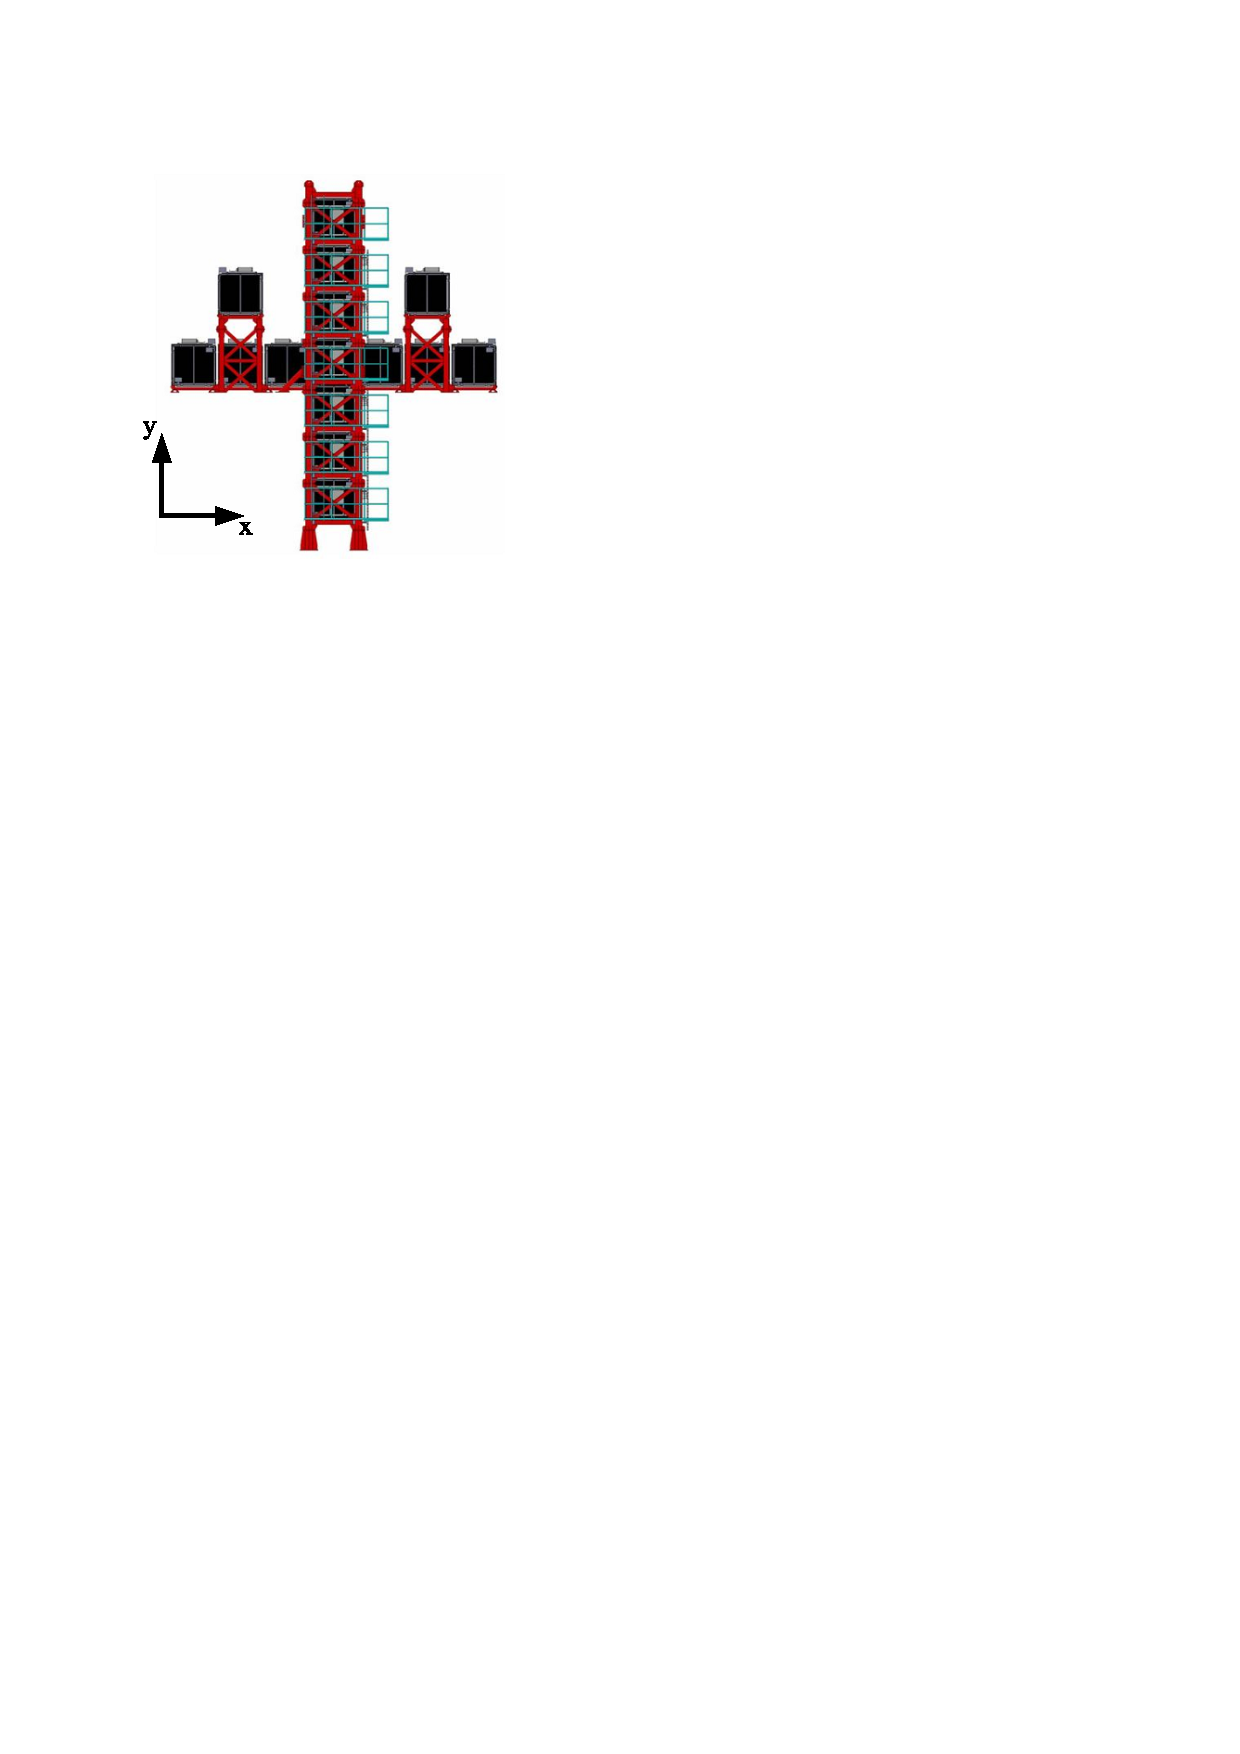
\includegraphics[width=6cm]{images/t2k/INGRID.pdf}
  \caption{A schematic of INGRID~\cite{Abe2011106}.}
  \label{fig:INGRIDSchematic}
\end{figure}
\newline
\newline
Each module consists of nine iron plates and 11 tracking scintillator planes in a sandwich structure.  The iron plates are 124~cm $\times$ 124~cm $\times$ 6.5~cm and provide 7.1~tons of target per module for the neutrino beam.  The scintillator planes provide tracking for the neutrino final-states and consist of scintillator bars threaded by WLS fibres and readout by MPPCs (see section~\ref{subsec:MPPC}).
\newline
\newline
This overall design allows INGRID to measure the beam centre to a 10~cm precision which corresponds to 0.4~mrad precision at the near detector complex~\cite{Abe2011106}.


\subsection{ND280}
\label{subsec:ND280}
ND280 (Near Detector at 280~m) is T2K's other near detector.  However, unlike INGRID, ND280 is positioned 2.5$^\circ$ off-axis to the neutrino beam.  ND280 is a heavy, fine-grained detector  which characterises the flux, energy spectrum and $\nu_e$ contamination of the $\nu_\mu$ beam and additionally makes neutrino cross-section measurements.  Because ND280 sits at the same off-axis angle as T2K's far detector, ND280's beam characterisation can be used to make signal and background predictions at the far detector.
\begin{figure}
  \centering
  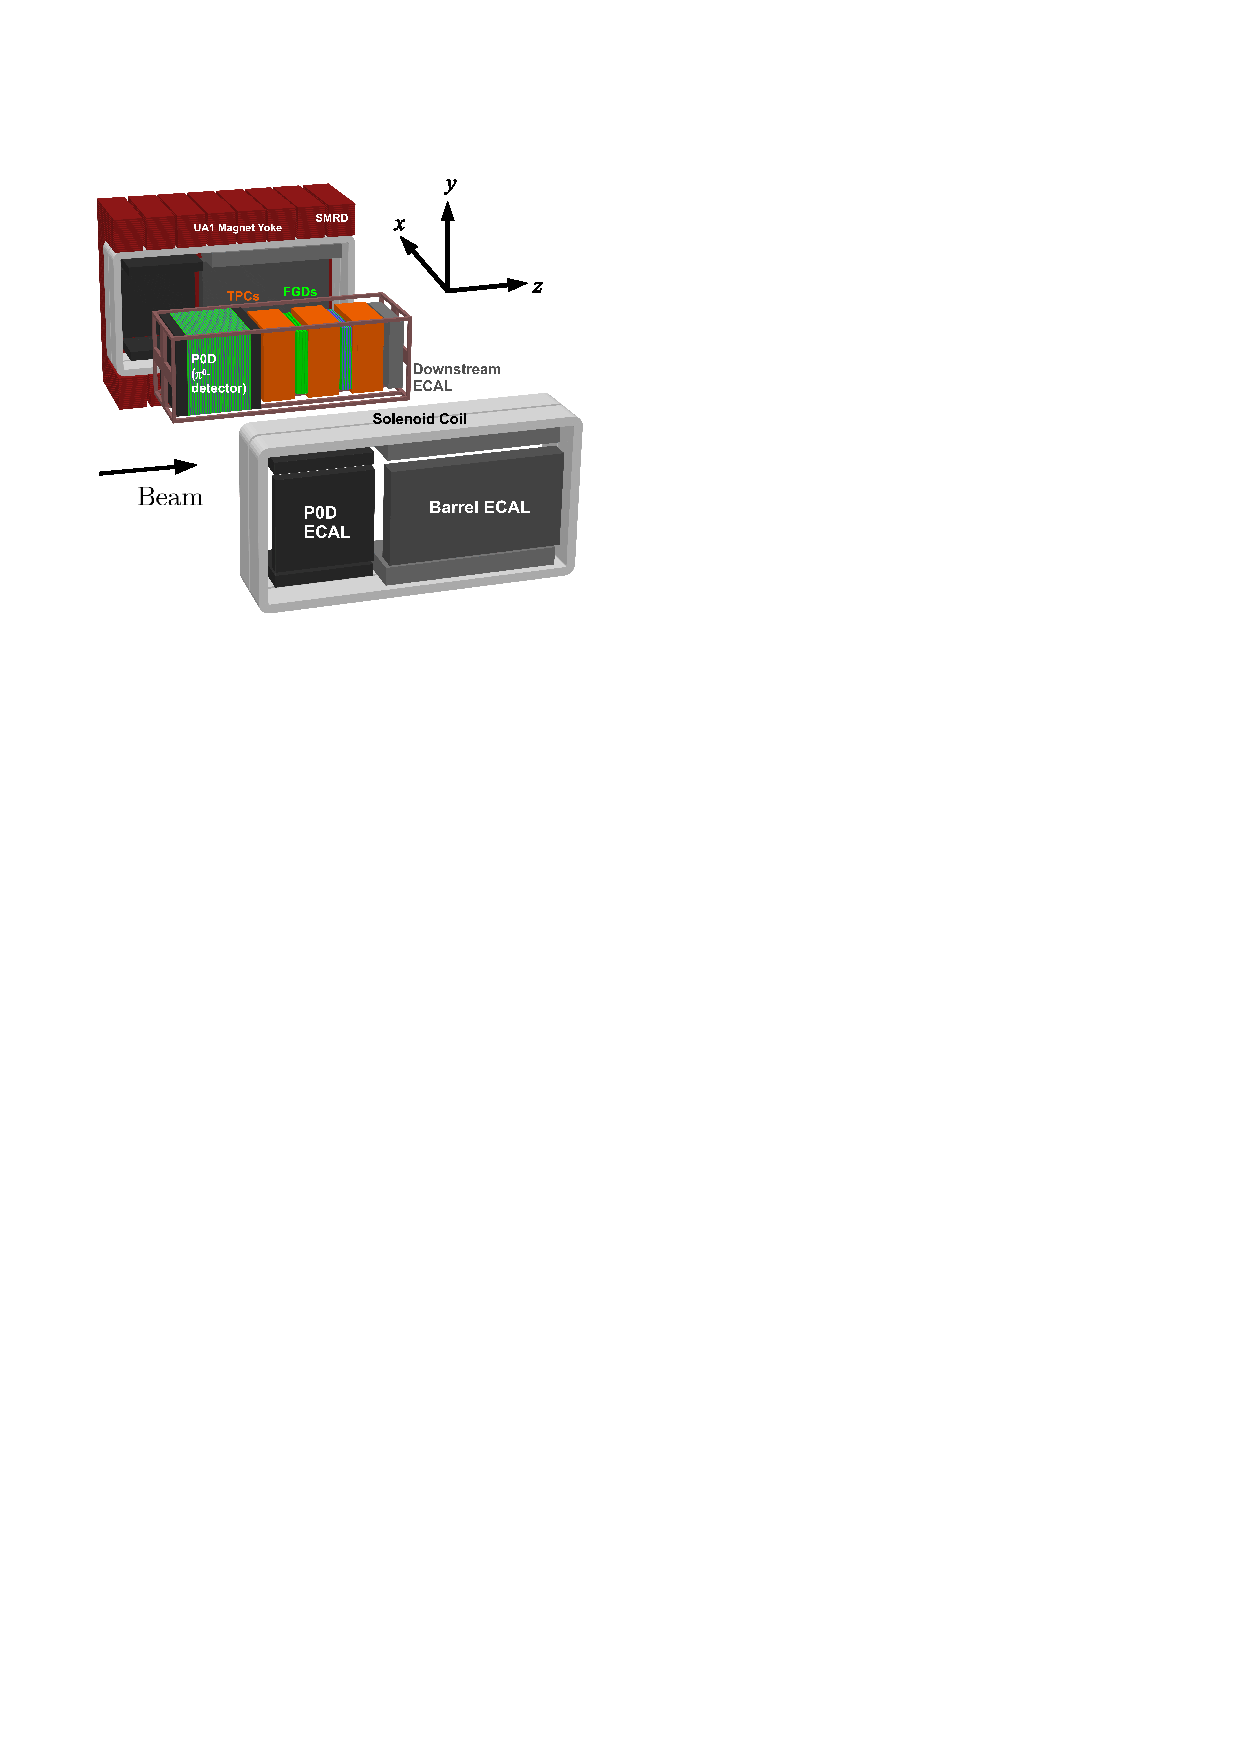
\includegraphics[width=9cm]{images/t2k/ND280Schematic.pdf}
  \caption{An exploded view of ND280~\cite{Abe2011106}.}
  \label{fig:ND280Schematic}
\end{figure}
\newline
\newline
Fig.~\ref{fig:ND280Schematic} shows an exploded view of the detector, which reveals the many subdetectors that form ND280.  The central tracking region comprises two Fine-Grained Detectors (FGDs~\cite{Amaudruz20121}) sandwiched between three Time Projection Chambers (TPCs~\cite{Abgrall201125}). The FGDs, which are composed of layers of plastic scintillator bars, provide the primary target for the neutrinos to interact with and the TPCs, filled with a gaseous mixture, allow for tracking of the charged final-states.  Essentially, the detectors in this region are complimentary and their combined information is used to reconstruct the majority of beam events relevant for oscillation analyses.  Upstream of the tracker region lies the $\pi^0$ detector (P$\O$D~\cite{Assylbekov201248}), whose design is optimised for studying neutrino interactions with $\pi^0$ in the final-state and consists of layers of scintillator, water and brass.  Surrounding the tracker and P$\O$D are a set of Electromagnetic Calorimeters (ECals~\cite{1748-0221-8-10-P10019}), primarily designed to detect particles originating from ND280's inner region.  Because particle identification is paramount to ND280's physics goals, all of the above detectors sit in a constant 0.2~T magnetic field, which is aligned with the $x$-axis in Fig.~\ref{fig:ND280Schematic}.  The magnetic return yoke and coils used to generate this field encompass the entire detector, allowing a constant field to be maintained within the detector, but greatly minimising the field's outside extent.  To maximise ND280's physics capability, the magnetic return yoke is instrumented with layers of plastic scintillator, which form the Side Muon Range Detectors (SMRDs~\cite{Aoki2013135}).


\subsubsection{The electromagnetic calorimeters}
\label{subsubsec:ecal}
The ND280 ECal is a lead-scintillator sampling calorimeter which consists of 13 modules separated into three distinct regions: the P$\O$D ECal which consists of six modules surrounding the P$\O$D, the barrel-ECal which is separated into six modules surrounding the tracker region and the DownStream-ECal (DS ECal) which is a single module located downstream of the inner detectors.  Motivated by their physics goals, the barrel-ECal and DS ECal are often considered together and will be referred to as the tracker ECal, while the P$\O$D ECal is considered a separate detector which is not used in this analysis and so will not be discussed further.  The primary physics goal of the ECal is to aide particle identification for final-states originating in the central region of ND280.  This is particularly important for interactions with $\pi^0$ in the final-state as the decay photons are difficult to identify using the tracker alone.
\newline
\newline
%All modules in the tracker ECal consist of layers of scintillating polystyrene bars with a 40~mm $\times$ 10~mm cross-section bonded to 1.75~mm lead sheets.
The barrel-ECals are separated into six modules: two modules above the tracker, two either side of the tracker and two below the tracker.  Each barrel-ECal module consists of layers of scintillating polystyrene bars with a 40~mm $\times$ 10~mm cross-section bonded to 1.75~mm lead sheets.  The scintillator bars provide a means of tracking the final-states while the lead sheets act as a radiator to produce electromagnetic showers and additionally provide a heavy mass neutrino target.  To measure the light readout, each scintillator bar has a 2~mm hole running through the centre in which a WLS fibre is inserted.  The fibre carries the light to the end of the bar where it can be collected by an MPPC.  The size of the gap between the tracker and the magnet placed a strong constraint on the size of barrel modules and so a scintillator bar thickness of 10~mm was chosen to minimise the ECal depth while maintaining a bar thickness which could provide sufficient light for signal capture.  The other key features of the active barrel-ECal volume (bar thickness, lead thickness and number of layers) were chosen to optimise particle identification and tracking.  A smaller bar width results in a detector with a higher resolution and studies investigating this found that the $\pi^0$ reconstruction efficiency was greatly compromised for $>$50~mm bar widths.  So, to facilitate costings, a compromise bar width of 40~mm was chosen.  The thickness of the lead absorber was also optimised based on the $\pi^0$ reconstruction efficiency.  The number of scintillator-lead layers was chosen such that electromagnetic showers of energy up to 3~GeV were adequately contained.  It was found that 10 electron radiation lengths ($X_0$) were required to ensure containment of at least 50$\%$ of $\pi_0$ decay photon showers.  So, this motivated a choice of 31 layers for all barrel-ECal modules which is equivalent to 9.7$X_0$.  For the purpose of 3D reconstruction, each ECal layer is oriented at 90$^\circ$ to the previous layer.  This means that in all barrel modules, there are 16 layers perpendicular and 15 layers parallel to the beam direction.  The perpendicular and parallel layers are slightly different, in that the scintillator bars are a different length.  In all barrel modules, the parallel bars are 3840~mm and are read out at both ends by separate MPPCs.  Because of the geometry, this is not the case for the perpendicular bars; the top and bottom module bar lengths are 1520~mm whereas the side module bar lengths are 2280~mm.  For all perpendicular bars, the signal is read out at one end only with the other end mirrored with aluminium to reflect the light.  Each barrel module is sandwiched between two carbon fibre plates and held in an aluminium frame which provides secure, structural support.
\newline
\newline
The DS ECal has almost identical features to that of the barrel in that it has scintillator bars with an identical chemical composition and cross-section while the lead absorbers are equally thick.  However, unlike the barrel-ECals, the DS ECal consists of 34 lead-scintillator layers which are, again, orientated at 90$^\circ$ to the previous layer.  Because of this, the DS ECal has a radiation length of 10.6$X_0$.  Additionally, every scintillator bar is 2000~mm and is read out at both ends by MPPCs.  Also, because of its position in the geometry, all layers are perpendicular to the beam direction.  The carbon fibre plates and aluminium frame are identical to those used in the barrel-ECal.
\newline
\newline
A summary of the tracker ECal design is shown in table.~\ref{table:ECalDesign}.
\begin{table}
\begin{center}
\begin{tabular}{l|l|l}
\hline
        & DS ECal  &Barrel ECal  \\ \hline
Length (mm)& 2300      & 4140   \\ 
Width (mm)  & 2300      & 1676  top/bottom \\ 
        &          & 2500 side  \\ 
Depth (mm)  & 500     & 462    \\
Weight (kg) & 6500 & 8000 top/bottom  \\
            &      & 10000 side        \\ \hline
Num. of layers &  34      &  31  \\ \hline
Bar orientation & $x/y$ &Para. and Perp. \\ \hline
Num. of bars    & 1700     & 2280 Para. top/bottom  \\ 
        &          & 1710 Para. sides \\     
        &          & 6144 Perp. top/bottom   \\ 
        &          & 3072 Perp. sides       \\ \hline  
Bars per layer & 50 & 38 Para. top/bottom\\
               &    & 57 Para. side\\
               &    & 96 Perp. top/bottom/sides  \\  \hline
Bar length (mm) & 2000  & 3840  Para. \\ 
           &      & 1520 Perp. top/bottom \\ 
           &      & 2280 Perp. sides      \\ \hline
Pb thickness (mm) & 1.75  & 1.75    \\ \hline 
\end{tabular}
\caption{Summary of the ECal design showing the overall dimensions, numbers of layers, length and orientation of the scintillator bars, numbers of bars, and lead thickness for each module~\cite{1748-0221-8-10-P10019}.}
\label{table:ECalDesign} 
\end{center}
\end{table}
\newline
\newline
The scintillator bars consist of polystyrene doped with 1$\%$~PPO and 0.03$\%$~POPOP and were extruded at a dedicated Fermilab facility.  During charge deposition, the PPO works as the primary scintillator and its output photons result in secondary scintillation of the POPOP.  This process acts as a wavelength shifter to produce an emission peak of 420~nm which matches the absorption peak of the 1~mm diameter WLS fibre threaded through the centre of the bar.  Every tracker ECal bar contains a 0.25~mm coating of polystyrene co-extruded with TiO$_2$ which provides reflection of the scintillation light.
\newline
\newline
The lead absorber layers consist of naturally occurring lead and stiffened with 2$\%$ antimony.  Traces of other metals are present but are below 0.15$\%$.  During construction, each lead layer was coated with a black, quick drying metal-conditioning primer to protect personnel from the toxic effects of the lead and to prevent leaching into the scintillator bars.  The lead layers themselves are actually constructed from multiple sheets rather than a single sheet largely due to ease of transportation.  In the case of the DS ECal, each layer consists of two 1008~mm $\times$ 2016~mm sheets.  For the top and bottom ECal modules, each layer consists of two 765~mm $\times$ 3858~mm sheets and the side module absorbers are constructed from four 2330~mm $\times$ 964.5~mm sheets.
\newline
\newline
The tracker ECal electronics system consists of several different readout boards.  All MPPCs are connected to a set of bespoke Trip-T\cite{Estrada:2003fh}\Yoshi{}{ADDRESSED - Need a citation for the trip-t boards} Frontend Boards (TFBs).  Each TFB comes with 64 channels to read out MPPCs which means that there are multiple TFBs associated with each ECal module.  All TFBs subsequently connect to Readout Merger Modules (RMMs) which act as the interface between the Data AcQuisition system (DAQ) and its associated TFBs.

\subsubsection{Data acquisition system}
\label{subsubsec:DAQ}
ND280 comes equipped with a DAQ which is responsible for triggering the readout of information from the subdetectors and subsequent storage.  Because of the low frequency of neutrino events, there are no strict trigger requirements which is in stark contrast to collider experiments.  So, there are only three triggers which are:
\begin{itemize}
\item \textbf{Beam trigger:} When a beam spill occurs, a timing signal is sent to the DAQ which issues a command to record ND280 data. 
\item \textbf{TRIP-t cosmic trigger:} If hits are seen on opposite sides of the outer detectors (allowed combinations are top and bottom SMRD, left and right SMRD, P$\O$D and DS ECal) which are outside of the beam time window, then the DAQ records data as the hits were likely caused by a cosmic ray muon.
\item \textbf{FGD cosmic trigger:} If hits are seen in both FGDs which are outside of the beam time window, then data is recorded as this was also likely to be caused by a cosmic ray muon.
\end{itemize}
The data is initially stored at KEK in Japan but is then replicated to TRIUMF in Canada and RAL in the UK for maximum redundancy and ease of access.

\subsection{The far detector}
The T2K experiment's far detector is Super-Kamiokande~\cite{Fukuda2003418}, which is a very large water Cherenkov detector containing 50~kton of ultra-pure water.  Positioned 295~km away from the J-PARC neutrino beam, SK is located under Mt.~Ikenoyama with a rock overburden of 1~km \Yoshi{(2.7~km water-equivalent)}{ADDRESSED - also put water equivalent}.  SK consists of two detectors; the inner detector consists of 11,146 inward facing 20\Yoshi{$''$}{ADDRESSED - was ''} PMTs which surround 35,000~ton of water while the outer detector consists of 1,885 outward facing 8\Yoshi{$''$}{ADDRESSED - was ''} PMTs and acts as a veto for entering backgrounds.
\newline
\newline
SK detects particles via Cherenkov radiation which is produced as a result of charged particles travelling in excess of the speed of light in the local medium.  This radiation is emitted at an angle of $\cos \theta = c/nv$, where $n$ is the refractive index of the material and $v$ is the speed of the particle.  For water this equates to an angle of 42$^\circ$.  The medium imposes a damping effect on the velocity of the particle, which results in energy loss and there comes a point where the Cherenkov emission condition is no longer met.  So, SK detects a ring of light emitted by the particles propagating through it.
\newline
\newline
The features of the Cherenkov ring are utilised for particle identification.  An electron, which showers upon creation in the water, creates a fuzzy ring of light while a muon, which cleanly propagates through the water, creates a sharp ring of light.  Examples of this are shown in Fig.~\ref{fig:SKPID} where the difference between muon and electron events can be clearly seen.
\begin{figure}
  \centering
  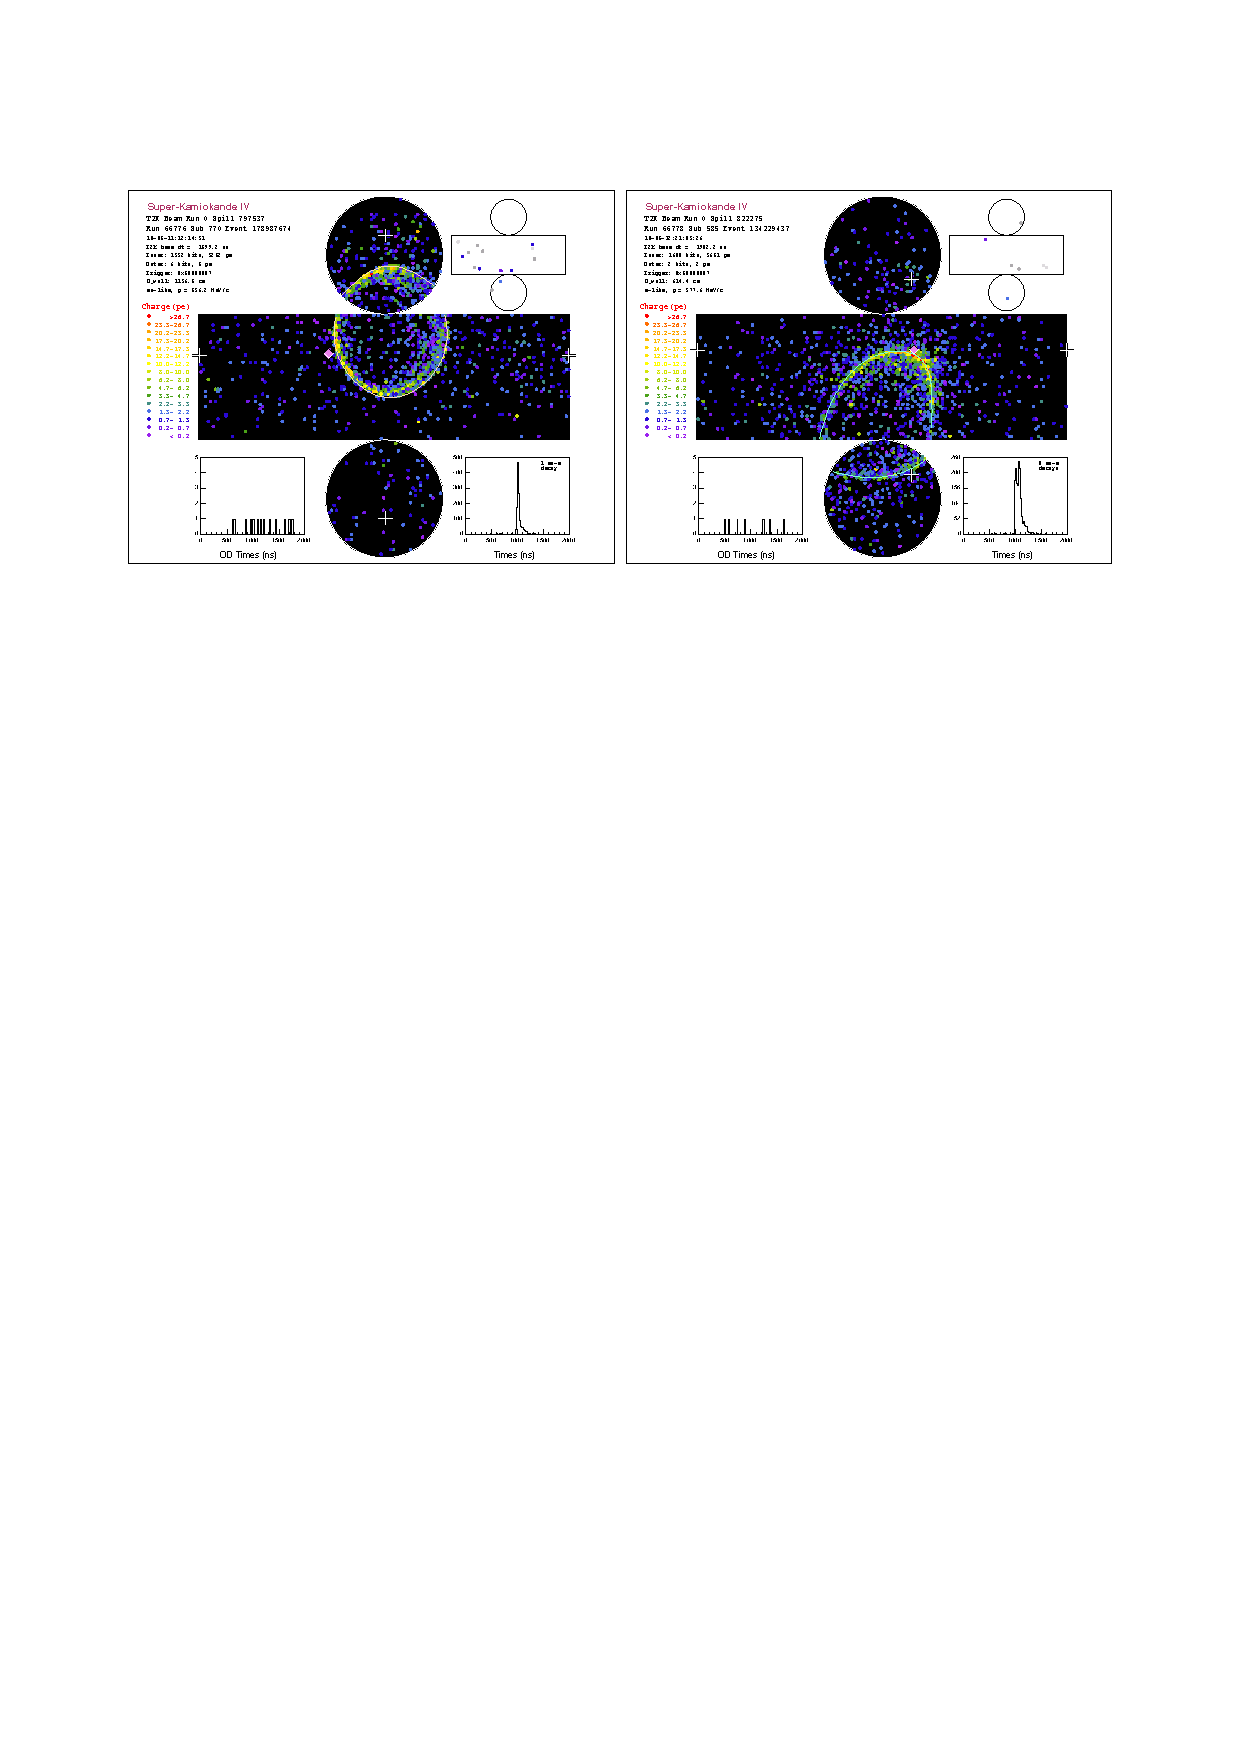
\includegraphics[width=9cm]{images/t2k/SK_PID.pdf}
  \caption{Example of reconstructed T2K events in SK for a muon-like ring (left) and an electron-like ring (right)~\cite{Abe2011106}.}
  \label{fig:SKPID}
\end{figure}

  %\chapter{ND280 software and existing ECal event reconstruction}
\label{chap:ND280Software}
The T2K experiment uses a bespoke software suite for simulation and analysis of ND280 data, which is based on the ROOT framework~\cite{Brun199781}.  The vast majority of the ND280 software suite utilises the oaEvent library which provides a unified framework for information manipulation and was specifically designed for this purpose.
As ND280 consists of many detector\Yoshi{}{ADDRESSED - check your apostrophes}s each providing a specific function, the ND280 software suite is designed to reflect this.  Not only are there specific software modules for individual subdetectors, there are specific modules for each phase of the subdetector information processing e.g. \Yoshi{Trip-T}{ADDRESSED - was trip-T. Be consistent with Chap 3} calibration, TPC reconstruction etc.  
\newline
\newline
As the software suite handles both production of simulated data and the processing of collected data, there are sections of the software chain which are specific to type of data being processed.  While the Monte Carlo simulation and real data do see different areas of the software chain, the general philosophy is to manipulate the Monte Carlo or the real data to a point where they can be treated as equals and them process them as such.  So, the description of the software will follow the same path: the Monte Carlo and real data specifics will be discussed first and then the unified treatment will follow. 
\section{Monte Carlo production software}
\label{sec:MCchain}
As described above, parts of the software chain are unique to simulated data processing.  Specifically, the simulation of the beam and the detector response need to be modelled before the Monte Carlo can be treated on equal footing with the real data.  This special processing is split into several steps, all of which are described below.

\subsection{Neutrino flux simulation}
\label{subsec:NeutrinoFluxSimulation}
The neutrino flux simulation uses Fluka2011~\cite{Ferrari_fluka:a} and a software set called JNUBEAM to model the J-PARC neutrino beam.  The process begins by using Fluka2011 to simulate the 30 GeV protons incident on the graphite target and their subsequent secondary interactions which produce the neutrinos parent mesons.  The kinematic information of the hadrons is then passed to the JNUBEAM simulation.  JNUBEAM is based on GEANT3~\cite{Brun:1987ma} and models the J-PARC secondary beamline.  The hadrons are tracked through the decay volume and are allowed to interact or decay to produce the simulated neutrino beam.  Importantly, all information associated with the daughter neutrinos and their parents are saved at this point.  By storing this information, the neutrino flux can be readily re-weighted to include new information associated with beam profile measurements or external data.
\newline
\newline
The main external tuning source is NA61/SHINE which is a hadron interaction experiment that uses a 31 GeV/c proton beam colliding with changeable targets~\cite{PhysRevC.84.034604}.  For use in the T2K flux simulation, NA61/SHINE has collected data using two graphite targets: one with a 4$\%$ nuclear interaction length thickness and a full T2K replica target.  The flux simulation used for this analysis is tuned using full replica target data.  Observed differences between the Fluka2011 simulation and NA61/SHINE data are used to re-weight the simulated neutrino flux.
\newline
\newline
Additionally to the external data, tuning measurements of the T2K beam profile are also used to re-weight the flux.  By making such measurements on a run-by-run basis, the simulated flux can be re-weighted to better model variations of the neutrino beam in each data run.
\subsection{Neutrino interaction simulation}
\label{subsec:NeutrinoInteractionSimulation}
After the neutrino flux has been modelled, simulation of the neutrino interactions with the T2K detectors follows.  The NEUT~\cite{Hayato2002171} event generator is used to simulate interactions with ND280.  The inputs to the interaction simulation are a neutrino vector file produced by the beam simulation and a ROOT based ND280 geometry.  The used geometry includes the magnetic field return yoke and everything contained within.  Using the inputs, NEUT tracks the neutrino and calculates the probability of interaction for every material it crosses.  To calculate the interaction probability, the potential interaction nucleus must be modelled.  For this, NEUT uses two models; the Moniz-Smith Relativistic Fermi Gas (RFG)~\cite{Miller2002223} and the O. Benhar spectral function models~\cite{Benhar1994493}.  The spectral functions are only implemented for carbon, oxygen and iron so the model used depends on the atomic number of the interaction candidate nucleus.  It is important to note at this point that this thesis deals with neutrino interactions on lead, so it is the RFG model that is used for signal interactions.
\newline 
\newline
The main interactions modes at T2K energies are quasi-elastic scattering (CCQE), single pion production  (CC1$\pi$) and Deep Inelastic Scattering (DIS) all of which have models in NEUT~\cite{LlewellynSmith1972261,Rein198179,1126-6708-2006-05-026}.
\newline
\newline
After the initial interactions, the final step is to simulate the final state interactions within the nucleus.  Each particle involved in the interaction is pushed through the nucleus in discreet steps with the probability of a final state interaction being calculated at each step.  If an interaction occurs, the final states of that interaction are also included in the subsequent steps.  This interactive procedure models the particle cascade until all the final states have reached the nucleus boundary.  At this point, all final state particles are recorded along with all of the information that created those particles.  This information is stored in a vector file and passed on to the ND280 detector MC package which handles the detector's response to these final state particles.
\newline
\newline
While the above description provides a general overview of the NEUT-based simulation of neutrino interactions, the above only describes simulation of NEUT events within the ND280 detector itself.  In reality, many interactions occur in the pit which surrounds the near detector, some of which have final state muons which enter ND280.  So, a separate NEUT-based simulation of neutrino interactions from the T2K beam in the ND280 pit and the surrounding substrate are also generated.  This kind simulation will be referred to as sand MC (because the interaction target is largely sand in the surrounding pit) from now on.
\subsection{ND280 detector simulation}
\label{subsec:ND280DetectorSimulation}
The simulation of the final state particles in ND280 is handled by nd280mc which is based on GEANT4~\cite{Agostinelli2003250} and ROOT.  The neutrino interaction vector files are taken as input and used as seeds in the detector simulation.  The neutrino vector inputs are not organised according to the J-PARC beam bunch structure so the detector simulation first groups the interactions into spills.  The beam intensity to be simulated is used to define how many interactions occur in a spill with Poisson fluctuations applied to that number.  The timing of the beam bunch structure is then used to group the interactions into bunches. 
\newline
\newline
nd280mc constructs a ROOT geometry of ND280 based on the design specifications of its subdetectors and then propagates the particles given to it by the neutrino generator through the geometry, simulating energy deposition, scattering and particle decay during propagation.
\newline
\newline
The sand MC is largely treated the same at this point; the surrounding pit geometry (and ND280) is constructed in nd280mc and the corresponding sand MC vectors provide the final state particles which are propagated by Geant4 through the geometry.  After this point, the sand MC is treated identically to the beam MC described above.

\subsection{Detector response simulation}
\label{subsec:DetectorResponseSimulation}
The next and final stage of the MC-only software chain is to model how the detector responds to the simulated particles propagating through it.  The detector response software, named elecSim, takes the output of nd280mc and models how the active regions of the detector would respond given an energy deposition in that region of the detector.  In the case of the calorimeters, elecSim handles the production of light produced by the constituent scintillator bars, how the light is propagated along the wavelength-shifting fibres and how the MPPCs would respond to the incident photons.  For the TPCs, the drift of the ionisation electrons through the gas and the subsequent response of the MicroMEGAS which receive them.  In all cases, the readout electronics response is simulated to produce a data-like output format.  This step concludes the section of the software chain which is specific to the MC.

\section{Real data processing software}
\label{sec:datachain}
The real data specific section of the software chain is very short.  Physics events deemed worth saving by any of the ND280 triggers are recorded by the detector and then saved for processing.  The MIDAS file format is used for storing the saved ND280 events.  All of the relevant information needed to process the event is stored in the MIDAS file, so the only unique step to the data processing is the conversion of the MIDAS file to the oaEvent format.  After the step, the oaEvent data files are exposed to the same software as MC files outputted by elecSim (see section~\ref{subsec:DetectorResponseSimulation}).


\section{Main software chain}
\label{sec:mainchain}
The aim of the rest of the software chain is to process the readout from the detector, be it simulated or collected data, and process it so essential information about the physics of the event can be extracted.  This is separated into three steps: calibration, reconstruction and data reduction/summarising.


\subsection{Detector calibration}
\label{subsec:DetectorCalibration}
The software package responsible for overseeing all aspects of the calibration stage is called oaCalib.  This controlling package passes the digitised signal from ND280 to dedicated calibration packages for the various kinds of readout electronics.  All of the information which can be extracted from an ECal event relies on the charge read by the MPPCs.  Thus, for the Trip-T detectors, like the ECals, the main aim of the calibration is to remove all electronic effects so that an accurate estimation of the charge read by the MPPCs can be made.  
\newline
\newline
Firstly, every MPPC is held at a bias in the absence of any signal to remove the non-linear dependence of the detector response on the lowest ADC channels.  This zero signal output is called the pedestal and must be subtracted from the charge readout by the MPPC.  
\newline
\newline
To estimate the number of photo-electrons produced in an MPPC, The readout charge is divided by the MPPC gain.  The breakdown voltage of an MPPC linearly varies with temperature (approximately 50 mV/$^\circ$C).  This translates to a percent level variation in the MPPC gain per degree.  This means small variations in temperature can cause a significant variation in the MPPC gain.  So, the gains for each channel are calculated and stored individually.
\newline
\newline
The time of the signal read by the MPPC is charge dependent and so it relies on the above corrections.  However, there are extra steps needed to get an accurate estimate of the timestamp.  The MPPC signal is given a timestamp once the charging capacitor exceeds a threshold value.  The time it takes to reach this threshold depends on the final collected charge of the MPPC.  This means that a lower charge signal would receive a later timestamp than a higher charge signal even if the signals occurred at the same time.  This effect is known as the electronic timewalk and is corrected for.
\newline
\newline
The light emission rate of the WLS fibres follows an exponential decay function which means that the emission rate depends on the total number of photo-electrons.  As described above, the Trip-T electronics only assign a timestamp once the collected charge passes a threshold.  So, the fibre decay causes a separate timewalk effect, called the fibre timewalk effect which is also corrected for.  
\subsection{Event reconstruction}
\label{subsec:EventReconstruction}
Once the information has been calibrated it is passed to the ND280 reconstruction software.  The reconstruction algorithms are separated into two phases: the local reconstruction and the global reconstruction.  The local reconstruction, which is run first, is separated into a set of algorithms specific to each subdetector.  Each subdetector reconstruction attempts to form its own picture of the event which passed through it.  After this, all of the local reconstruction information is passed to the global reconstruction which attempt to match and refit the subdetector results to maximise the amount of extractable information.

\subsection{Data reduction and summarising}
\label{subsec:DataReduction}
The final stage of the processing chain is to reduce and summarise all of the previous steps in the chain such that they are in a suitable format for the analyser.  A lot of the information, particularly from the reconstruction stage, is stripped out and the physics related objects are extracted.  Most importantly, all of the information is summarised in a pure ROOT format, meaning the analyser does not rely on the oaEvent library to analyse ND280 data.


\section{ECal event reconstruction}
\label{sec:ECalEventReconstruction}
As mentioned in section~\ref{subsec:EventReconstruction}, part of the reconstruction process is to run algorithms specific to the ND280 subdetectors.  The ECal is no exception and is equipped with an extensive suite of reconstruction algorithms designed to reconstruct events originating from the Tracker region of ND280.  The inputs to the reconstruction are the calibrated scintillators bar hits which are used to form 3D objects and attach a topology hypothesis.

\subsection{Hit preparation}
\label{subsec:ECalHitPerparation}
The initial ECal reconstruction stage takes the hits outputted by the calibration stage and prepares them for the downstream algorithms.  The ECal hits arrive with timestamps but are not separated according to the bunch structure.  So, the hits are ordered in time and then grouped into buckets where a new bucket starts when a greater than 50~ns gap appears between two time-adjacent hits.  A second filter is then applied to arrange the hits according to the sensor they occurred on.  For double ended bars with both sensors activated, the time of the hit is re-estimated by averaging the timestamp of the two sensors.  The two hits are then merged to form a single hit.
\newline
It is then necessary to apply extra calibrations to the charges of the hits.  The effect of light attenuation along the WLS fibre is corrected for and a scaling is applied to convert the charge into MIP equivalent units (MEU)\YoshiFinal{}{Can you briefly explain what an MEU is, and reference it? It isn't standard terminlogy}.

\subsection{Basic clustering}
\label{subsec:ECalBasicClustering}
The time ordered hits are then passed to a set of clustering algorithms which attempts to form an object out of the ECal hits.  The first stage of this is called basic clustering which is a nearest neighbour algorithm designed to form 2D clusters of hits for both views of an ECal module.  This is initiated by forming a 30 ns window and searching for the highest charge hit contained within it to form a seed.  The seed cluster is expanded by searching for and adding candidate hits which pass the following criteria:
\begin{itemize}
  \item Is located in the 30 ns time window
  \item Is at most one bar away from a hit in the cluster
  \item Is at most two layers away from a hit in the cluster
\end{itemize}
To qualify as a basic cluster, any formed candidate must contain at least three hits.  The successfully formed clusters in both views of the ECal modules are then passed to the next stage of the clustering algorithms. 

\subsection{Cluster combination}
\label{subsec:ECalCombineClusters}
The second stage of the clustering algorithm takes the basic clusters in a given view and attempts to form merged clusters if a set of conditions are passed.  The cluster with the highest number of hits is taken as a seed and compared with all other clusters in the same view.  A Principal Components Analysis (PCA) is applied to all 2D clusters as the primary axis is used in one of the merging criteria.  A candidate cluster is merged with the seed cluster if:
\begin{itemize}
  \item The distance of closest approach, taken from the primary axes, of the candidate and seed cluster is less than 80~mm
  \item The charge weighted average hit times of the candidate cluster is within 40 ns of the seed cluster
  \item The charge weighted average distance of the candidate cluster to the seed cluster is less than 400~mm
\end{itemize}
All candidate clusters which pass the conditions are merged with the seed cluster.  After all comparisons have been made, a new seed cluster is found and the process is repeated until no more merges take place.  All clusters in each ECal view are then passed into the next clustering algorithm.



\subsection{Cluster expansion}
\label{subsec:ECalExpandClusters}
The next and final stage of the 2D clustering attempts to merge any unmatched hits with the already formed clusters if the comparison passes a set of conditions.  As before, a PCA is applied to all 2D clusters to calculate the primary and secondary axes as, again,  these are used in one of the matching conditions.  Let $\vec{n}_{\mathrm{pri}}$ and $\vec{n}_{\mathrm{sec}}$ be the primary and secondary axes of a cluster found by the PCA.  The squared spread of the cluster along the primary or secondary axis is then defined as
\begin{equation}
  \sigma_A^2 = \sum_{\alpha = x,y,z} \sigma_\alpha^2n_{A,\alpha}^2,
\end{equation}
where $A$ refers to either the primary or secondary axis and $\sigma_\alpha$ refers to the cluster's spread along the Cartesian axes.  A metric for defining how well the hit matches to the cluster can then be defined as 
\begin{equation}
  w = \sqrt{\Bigg(\frac{\vec{H}\cdot \vec{n}_{\mathrm{pri}}}{\sigma_{\mathrm{pri}}}\Bigg)^2 +  \Bigg(\frac{\vec{H}\cdot \vec{n}_{\mathrm{sec}}}{\sigma_{\mathrm{sec}}}\Bigg)^2},
\end{equation}
where $H$ is the vector joining the charge-weighted centre of the cluster and the centre of the hit.  The unmatched hit is merged with the 2D cluster if:
\begin{itemize}
  \item The unmatched hit is within 6 ns of one of the constituent hits of the 2D cluster
  \item The difference in bar number of the unmatched hit and at least one of the constituents hits in the 2D cluster is less than 11
  \item The difference in layer number of the unmatched hit and at least one of the constituents hits in the 2D cluster is less than 21
  \item The calculated value of $w$ is less than 50
\end{itemize}
Unlike the previous stage where it is possible to merge every cluster in a view, an unmatched hit can be matched with one, and only one, 2D cluster. So, not only does the hit-cluster comparison have to pass the relevant criteria, the comparison has to be a better match than all other comparisons.  In cases where the unmatched hit passes all of the conditions with more than one cluster, the comparison which provides the lowest $w$ is selected as the best match.
\newline
\newline
The 2D clusters in each view are then passed on to the final stage of the clustering algorithms.

\subsection{3D cluster formation}
\label{subsec:ECal3DMatching}
The final stage of the clustering algorithm attempts to form full 3D clusters using information from both view of an ECal module.  To do this, the algorithm takes the 2D clusters from one view and matches them with the 2D clusters in the other view.  All 2D clusters from one view are compared to all 2D clusters in the other view and the two that are the best match form a 3D cluster.  The metric used for the matching is a simple likelihood based on three input variables.  The first variable is the ratio of the total charge of the 2D matching candidate clusters, $Q_{\textrm{ratio}}$.  Assuming the two 2D clusters come from the same particle, the amount of charge deposited in each view should be similar, so $Q_{\textrm{ratio}}$ should be \sim1.  The $Q_{\textrm{ratio}}$ value is then compared with a probability density function generated using ND280 MC to retrieve $\mathcal{L}_{Q_{\textrm{ratio}}}$.  The second input variable to the likelihood compares the first layer used by the two matching candidate clusters which is closest to the ND280 Tracker region, $\Delta_{\textrm{layer, first}}$.  If the two candidate clusters are created from the same particle, the difference in starting layer number should ideally be one.  As with with $Q_{\textrm{ratio}}$, the $\Delta_{\textrm{layer, first}}$ found for the matching candidates is compared to a probability density function to retrieve $\mathcal{L}_{\Delta_{\textrm{layer, first}}}$.  The final input to the likelihood is almost identical to the second input.  The variable, called $\Delta_{\textrm{layer, last}}$ compares the difference in layer number furthest away from the ND280 Tracker region.  Besides this difference, $\Delta_{\textrm{layer, last}}$ is treated in exactly the same manner as $\Delta_{\textrm{layer, first}}$ and so will not be described in any more detail.
\newline
Once the three inputs for the matching candidates have been calculated, the value of the matching likelihood is then
\begin{equation}
  \mathcal{L} = \mathcal{L}_{Q_{\textrm{ratio}}} \times \mathcal{L}_{\Delta_{\textrm{layer, first}}} \times \mathcal{L}_{\Delta_{\textrm{layer, last}}}.
\end{equation}
As mentioned above, all 2D clusters in one view are compared with all 2D clusters in the other view.  The matching pair which produce the highest value of $\mathcal{L}$ are counted as a match.  The matched pair are then removed from the pool and the process is repeated until no more matches can be made or the value of $\mathcal{L}$ falls below $e^{-5}$.  All matched clusters are now counted as 3D objects and are passed on to the rest of the ECal reconstruction algorithms.

\subsection{3D hit reconstruction}
\label{subsec:ECal3DHitReconstruction}
So far in the ECal reconstruction, it has only been possible to reconstruct 2/3 of the hit coordinates.  However, now that full 3D clusters have been formed, the information from both ECal views can be used to estimate the third hit coordinate which is the coordinate along the length of the bar.
\newline
\newline
The hits are separated into their respective 2D view and then the charge-weighted average position of each layer is calculated.  Then, to calculate the final hit coordinate, the nearest four layers from the other view are found and a linear least-squares fit is applied to their 2D coordinates.  The line found is then extrapolated into the layer of interest which provides the unknown hit coordinate.

\subsection{Energy reconstruction}
\label{subsec:ECalEnergyReconstruction}
The ECal was designed to catch electromagnetic particles originating from the Tracker region of ND280, particularly photons from $\pi^0$ decays.  An integral part of particle shower reconstruction is estimation of the total energy of the incoming particle.  So, the next phase of the reconstruction is particle energy estimation under the assumption that the incident particle created a full contained particle shower upon entering the ECal module.  The range of the energy fitter is 25 MeV to 20 GeV which almost fully covers the range of energies seen in the ND280 ECals.  The energy fitter works by minimising a likelihood function which takes the total charge, charge RMS and charge skew of the 3D cluster as inputs.  For each of the three input variables, splines were generated using simple photon particle gun MC which relates the input variables to the true particle energy.  The minimizer generates an estimate of the true energy and, via the splines, retrieves the expected values of the input variables.  By minimising the distance between the measured input variables and those taken from the splines an accurate estimate of the particle energy is found.  This energy estimate, along with the 3D cluster itself, is then passed on to the final section of the ECal reconstruction.

\subsection{Event classification}
\label{subsec:ECalParticleIdentification}
The final section of the ECal reconstruction is to attach a topology hypothesis to the 3D cluster.  The routines currently separate the clusters into two categories: those that are shower-like and those that are track-like using an Artificial Neural Network (ANN).  This multi-variate analysis object takes multiple pieces of information about the 3D cluster which attempts to measure the energy deposition and shape of the cluster and returns a single number.  The value of the returned number suggests whether the reconstructed object is track-like or shower-like. The discriminator was tested using ND280 electron and muon control samples, the results of which are shown for the DS ECal in Fig.~\ref{fig:ECalTrShVal}.

\begin{figure}
  \centering
  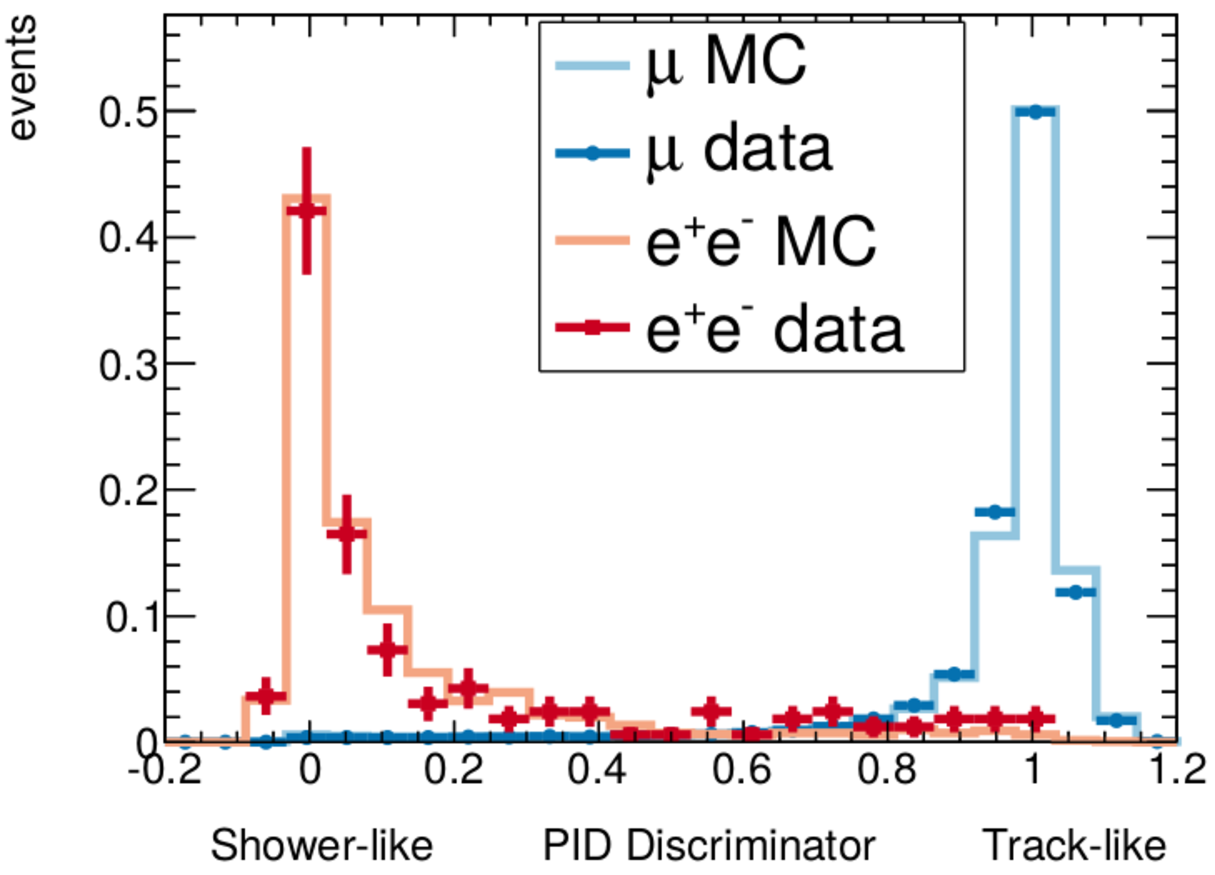
\includegraphics[width=11cm]{images/software/ecal_trshval.pdf}
  \caption{The track-like/shower-like discriminator for the DS ECal which is uses an Artificial Neural Network~(ANN)~\cite{1748-0221-8-10-P10019}.  Solid lines show the control sample Monte Carlo (based on NEUT simulation of beam events) and the points show the control sample data (taken from collected beam data).  For the muon samples, exactly one track is required in each of the TPCs and the DS ECal with an additional requirement that the TPC tracks are muon-like.  For the electron samples, photon pair production is checked in the FGD, requiring tracks with opposite charge with at least one TPC track which must be electron-like.  The muon and electron simulated distributions show good agreement with the collected data.\Yoshi{}{ADDRESSED - Say which reconstruction this comes from, and what the data and MC represent. The original caption carries way too little info}}
  \label{fig:ECalTrShVal}
\end{figure}



  %\begin{sidewaysfigure}
%  \begin{center}
%  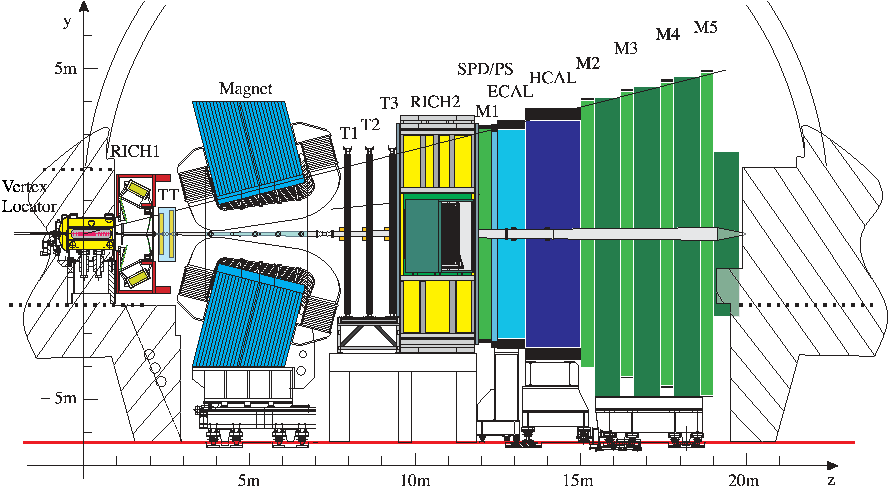
\includegraphics[width=0.8\textheight]{lhcb-detector-cross-section}
%  \caption[Cross-section view of \LHCb, cut in the non-bending $y$--$z$ plane]%
%    {Cross-section view of \LHCb, cut in the non-bending $y$--$z$ plane.}
%  \label{fig:LHCbCrossSection}
%  \end{center}
%\end{sidewaysfigure}



\chapter{Enhanced ECal reconstruction}
\label{chap:EnhancedECalReconstruction}
The current implementation of the ECal reconstruction software was designed to reconstruct particles which originate from the ND280 tracker and enter the ECal.  As section~\ref{sec:ECalEventReconstruction} shows, this was realised by only considering reconstructed ECal clusters under the single track-like or shower-like hypothesis.  It should be evident that a neutrino interaction occurring within the ECal does not well fit this topology.  While it is true that there is some power in the current reconstruction to distinguish a neutrino interaction from an entering track or shower, there is little feature information available.  How many final state particles propagated from the interaction?  How much visible energy was deposited by each of the particles?  Where in the ECal did the interaction occur?  These basic questions can not be trivially answered when using the current reconstruction.  To maximise the ability of distinguishing ECal neutrino interactions from entering backgrounds, the reconstruction must be revisited.

\section{The Hough transform}
\label{sec:HoughTransform}
The Hough transform is a popular method of machine pattern recognition used by, but is not limited to, high energy physics experiments.  Originally designed for machine track recognition in bubble chamber pictures~\cite{Hough:1959qva}, the version most widely used throughout the world was developed in 1972~\cite{Duda:1972:UHT:361237.361242}.  The Hough transform is used to isolate specific features or shapes from a digital image.  The simplest implementation, which is of most interest in event reconstruction, allows the extraction of straight 2D lines from a complex pattern.  This is acheived by exploitation of a simple, but remarkable, feature of 2D geometry.

\subsection{Line-point duality}
\label{subsec:LinePointDuality}
Consider a straight line formed in a 2D cartesian space as shown in Fig.~\ref{fig:2DCartesianLine}.  The line is usually described by
\begin{equation}
  y = mx + c
  \label{eq:2DLineCartesean}
\end{equation}
where $y$ and $x$ are used as coordinates, $m$ is the gradient of the line and $c$ is the intercept location of the line with the $y$ axis.  While it is not necessary to analyse this simple shape in great detail, it is important to note that $m$ and $c$ are the only parameters necessary to completely describe the line.  
\newline
\newline
Now consider a new 2D space where the axes are defined by $m$ and $c$, rather than $x$ and $y$ (hereafter referred to as the parameter space).  As this parameter space is described by the parameters of a general 2D cartesian line, there is an underlying symmetry between the two spaces.  The parameters of the 2D line shown in Fig.~\ref{fig:2DCartesianLine} can be used to form a pair of coordinates ($m$,$c$) in the parameter space as shown in Fig.~\ref{fig:2DParameterPoint}.  It is important here to state clearly the general result; a straight line in cartesian space is represented by a single point in parameter space. 
%\begin{figure}
%  \centering
%  \parbox{7cm}{
%    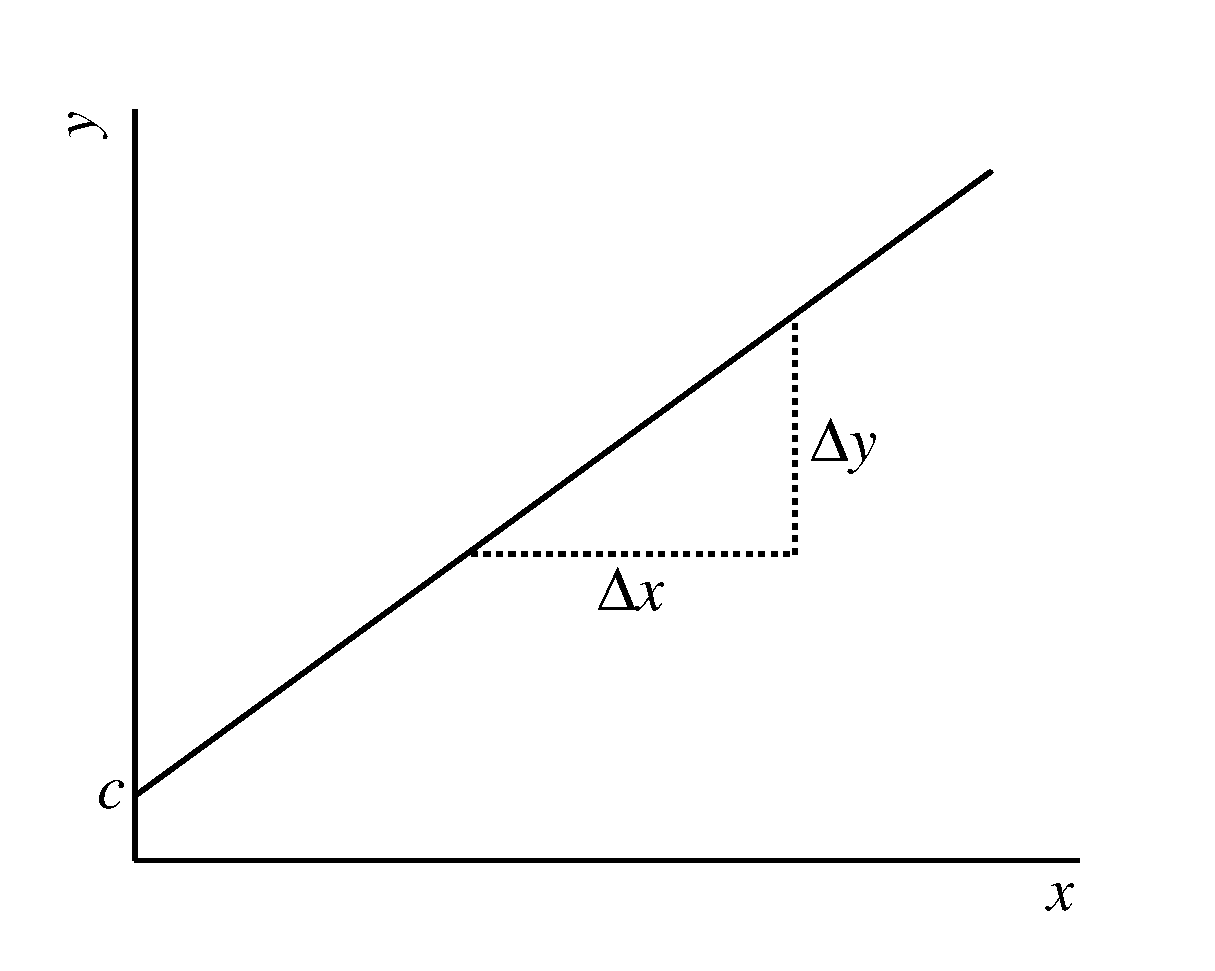
\includegraphics[width=7cm]{images/hough_transform/cartesian_line}
%    \caption{Line in 2D cartesian space.}
%    \label{fig:2DCartesianLine}}
%    \qquad
%    \begin{minipage}{7cm}
%      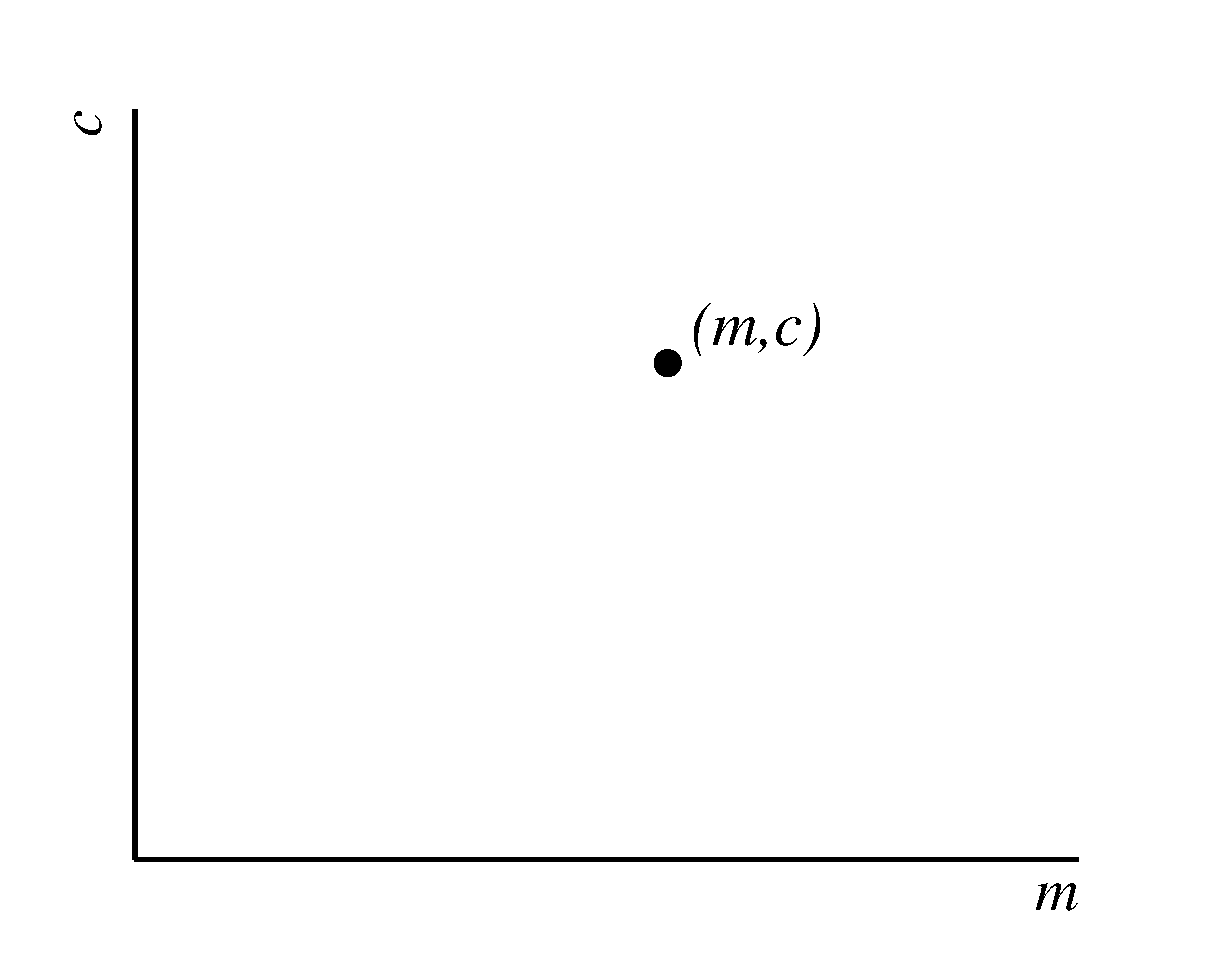
\includegraphics[width=7cm]{images/hough_transform/parameter_point}
%      \caption{Point in 2D parameter space.}
%      \label{fig:2DParameterPoint}
%    \end{minipage}
%\end{figure}
\begin{figure}%
  \centering
  \subfloat[Line in 2D cartesian space.]{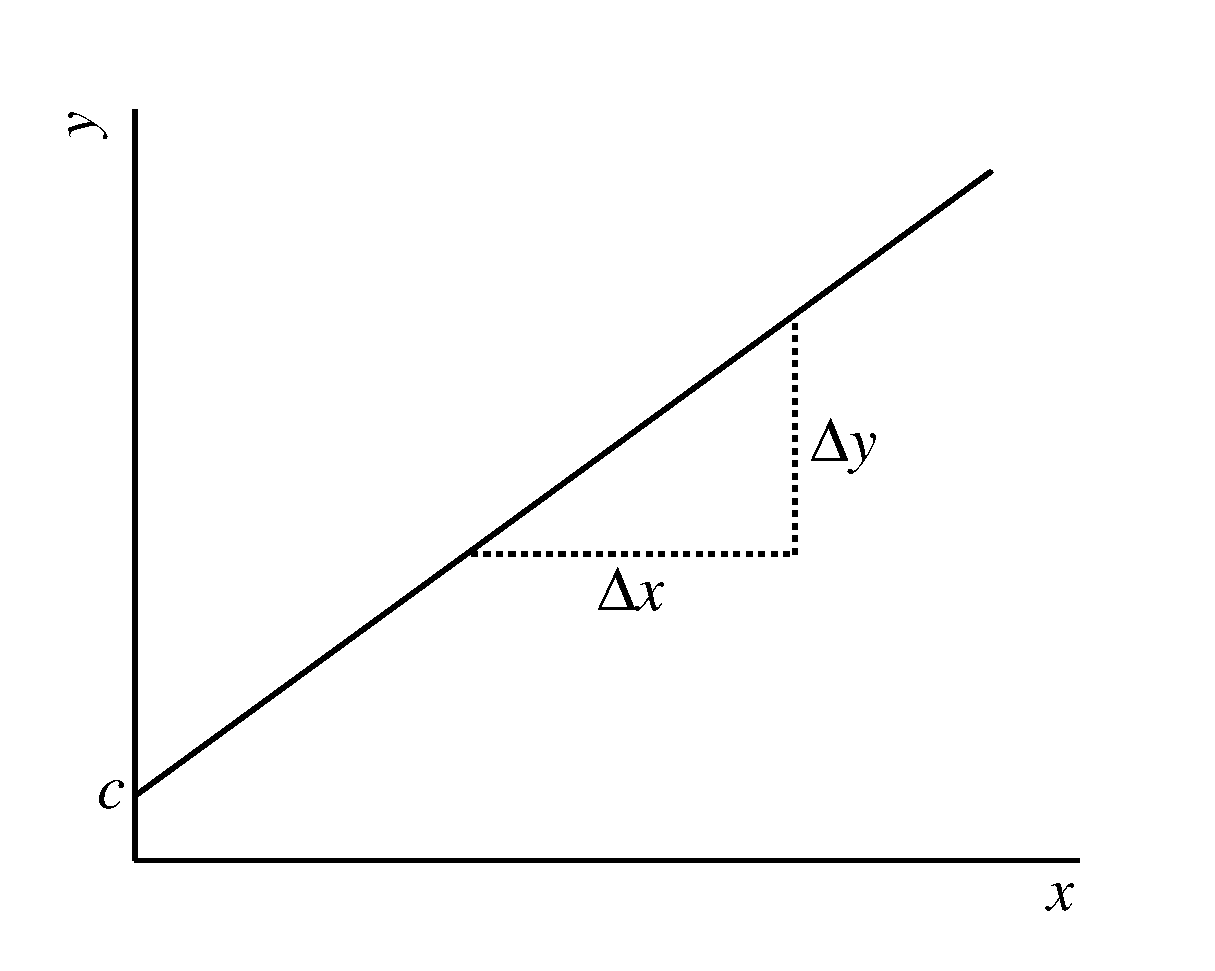
\includegraphics[width=7cm]{images/hough_transform/cartesian_line} \label{fig:2DCartesianLine}}
  \subfloat[Point in 2D parameter space.]{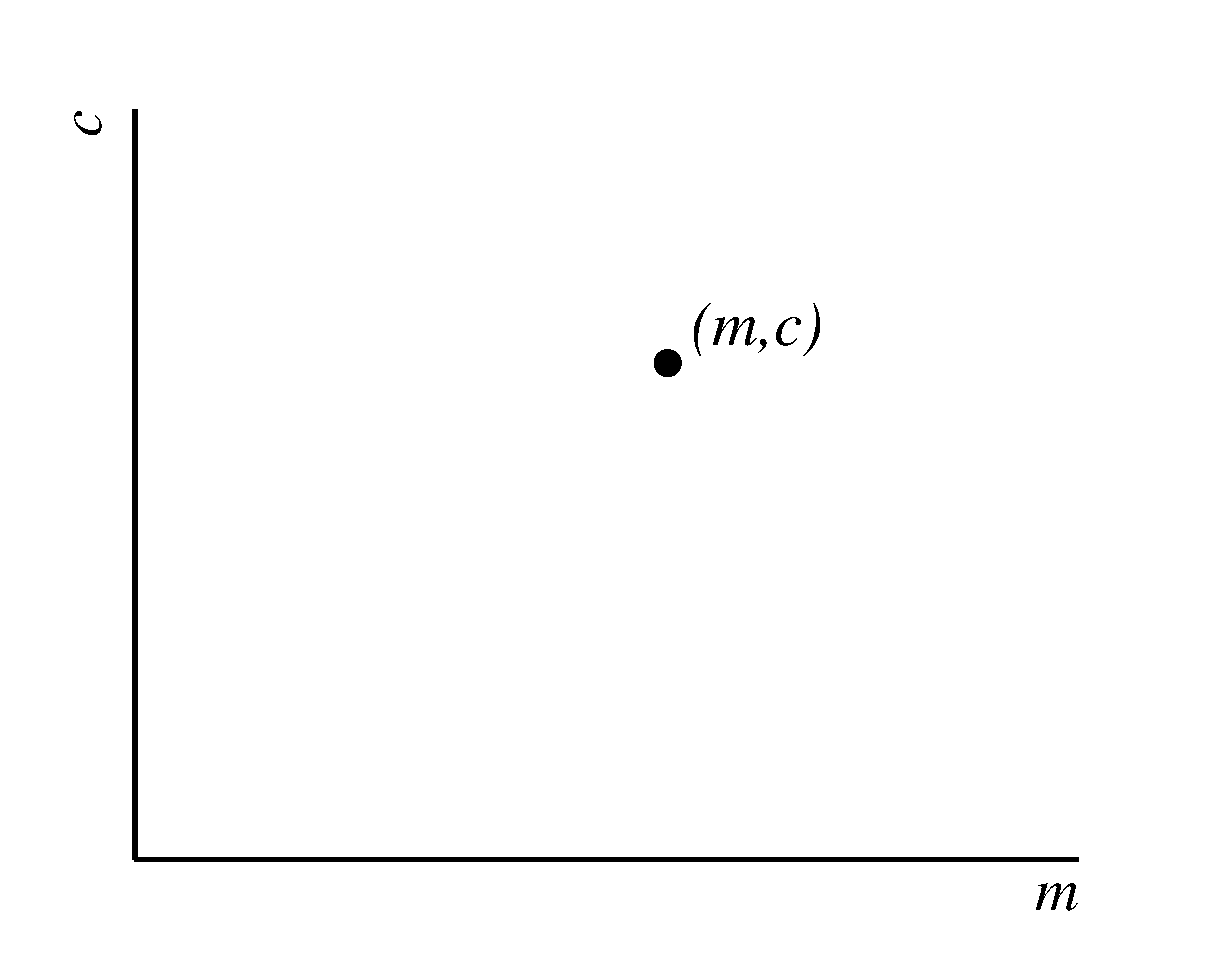
\includegraphics[width=7cm]{images/hough_transform/parameter_point} \label{fig:2DParameterPoint}}
  \caption{Representations of a 2D line in cartesian space.}
  \label{fig:2DCartesianLineAndParameterPoint}
\end{figure}
\newline
\newline
Now consider the 2D cartesian space again.  Unlike before, we will define a single point rather than a straight line. Such a point is traditionally described by a pair of coordinates ($x$,$y$).  However, an alternative description of the point is an infinite number of lines all of which pass through ($x$,$y$).  This is highlighted by Fig.~\ref{fig:2DCartesianPoint} where three lines of the infinite set are shown along with the point they represent.  As the infinite line set are used to describe a single point, all lines in the set must follow a pattern.  This relationship is revealed by simple algebraic manipulation of equation~\ref{eq:2DLineCartesean} to give
\begin{equation}
  c = -xm + y.
  \label{eq:2DLineParameter}
\end{equation}
Despite the manipulation, equation~\ref{eq:2DLineParameter} still resembles the equation of a 2D line, however the parameters are $x$ and $y$ and the coordinates are $m$ and $c$.  Specifically, equation~\ref{eq:2DLineParameter} is represented by a line in the parameter space defined above.  The gradient of this line is 
\begin{equation}
  x = \frac{\Delta c}{\Delta m}
  \label{eq:2DLineGradientParameterSpace}
\end{equation}
and the intercept of the line with the $c$ axis is $y$ as shown in Fig.~\ref{fig:2DParameterLine}.  As before, it is important to clearly state what has been shown; a point in cartesian space is represented by a line in parameter space.
%\begin{figure}
%  \centering
%  \parbox{7cm}{
%    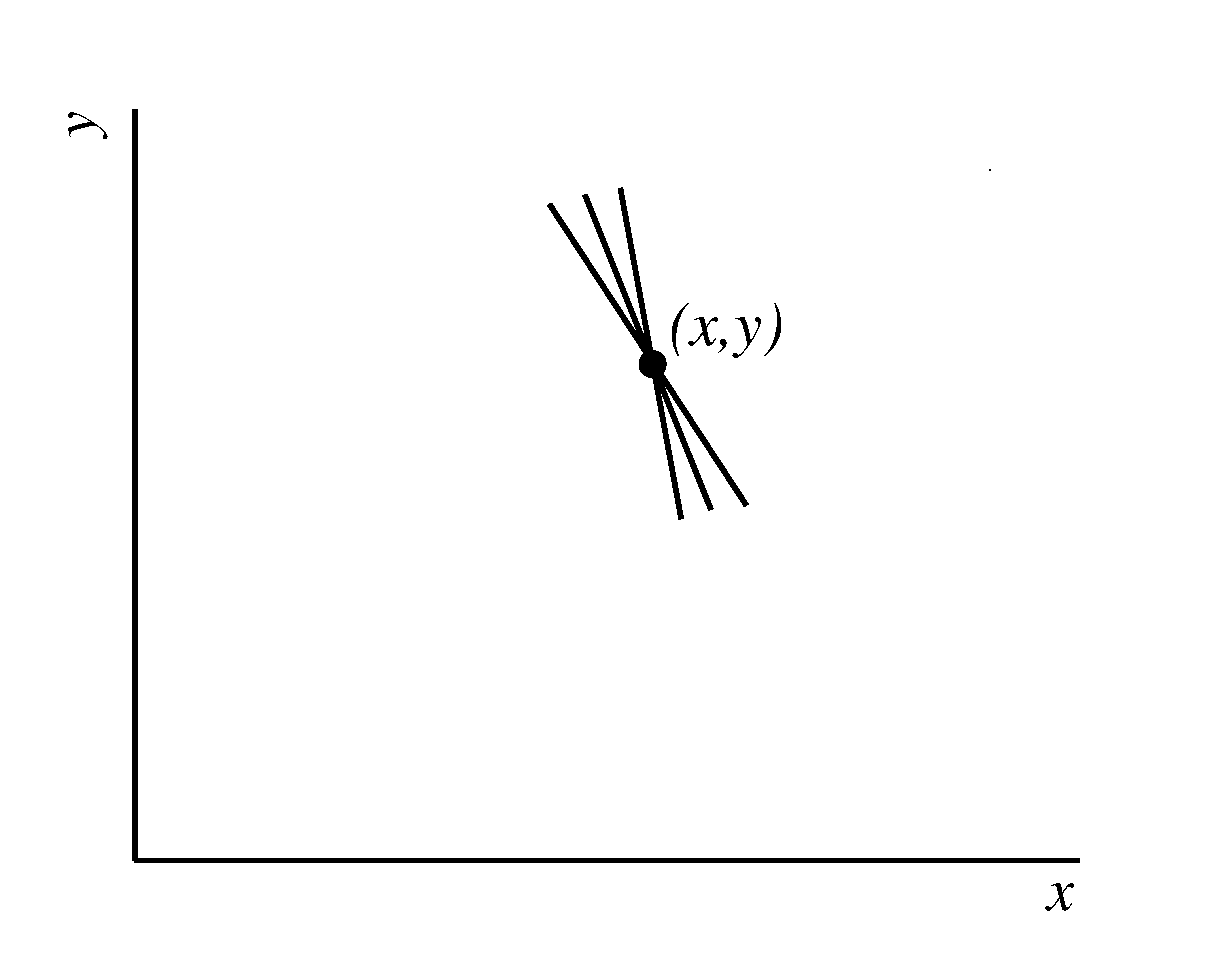
\includegraphics[width=7cm]{images/hough_transform/cartesian_point}
%    \caption{Point in 2D cartesian space.}
%    \label{fig:2DCartesianPoint}}
%    \qquad
%    \begin{minipage}{7cm}
%      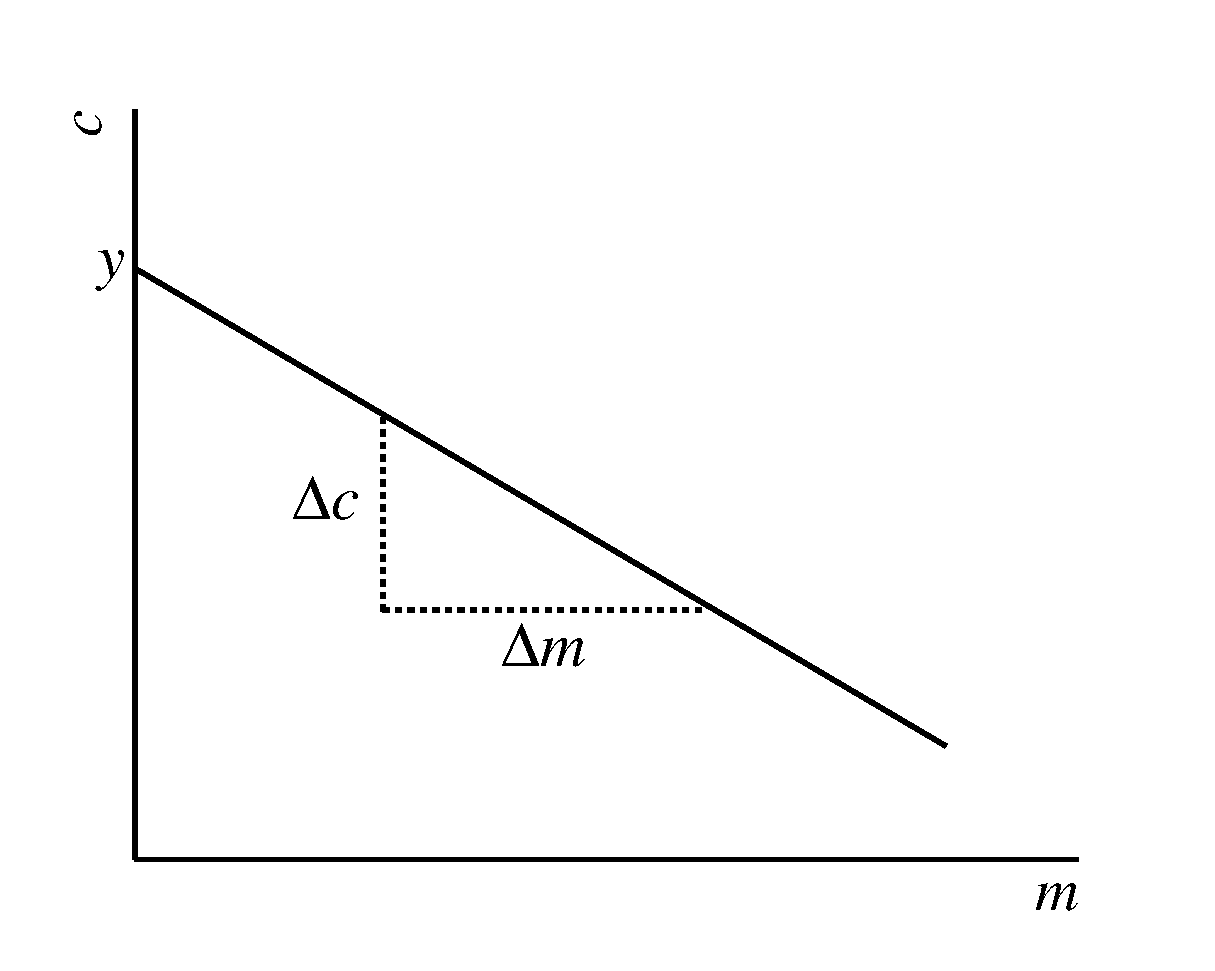
\includegraphics[width=7cm]{images/hough_transform/parameter_line}
%      \caption{Line in 2D parameter space.}
%      \label{fig:2DParameterLine}
%    \end{minipage}
%\end{figure}
\begin{figure}%
  \centering
  \subfloat[Point in 2D cartesian space.]{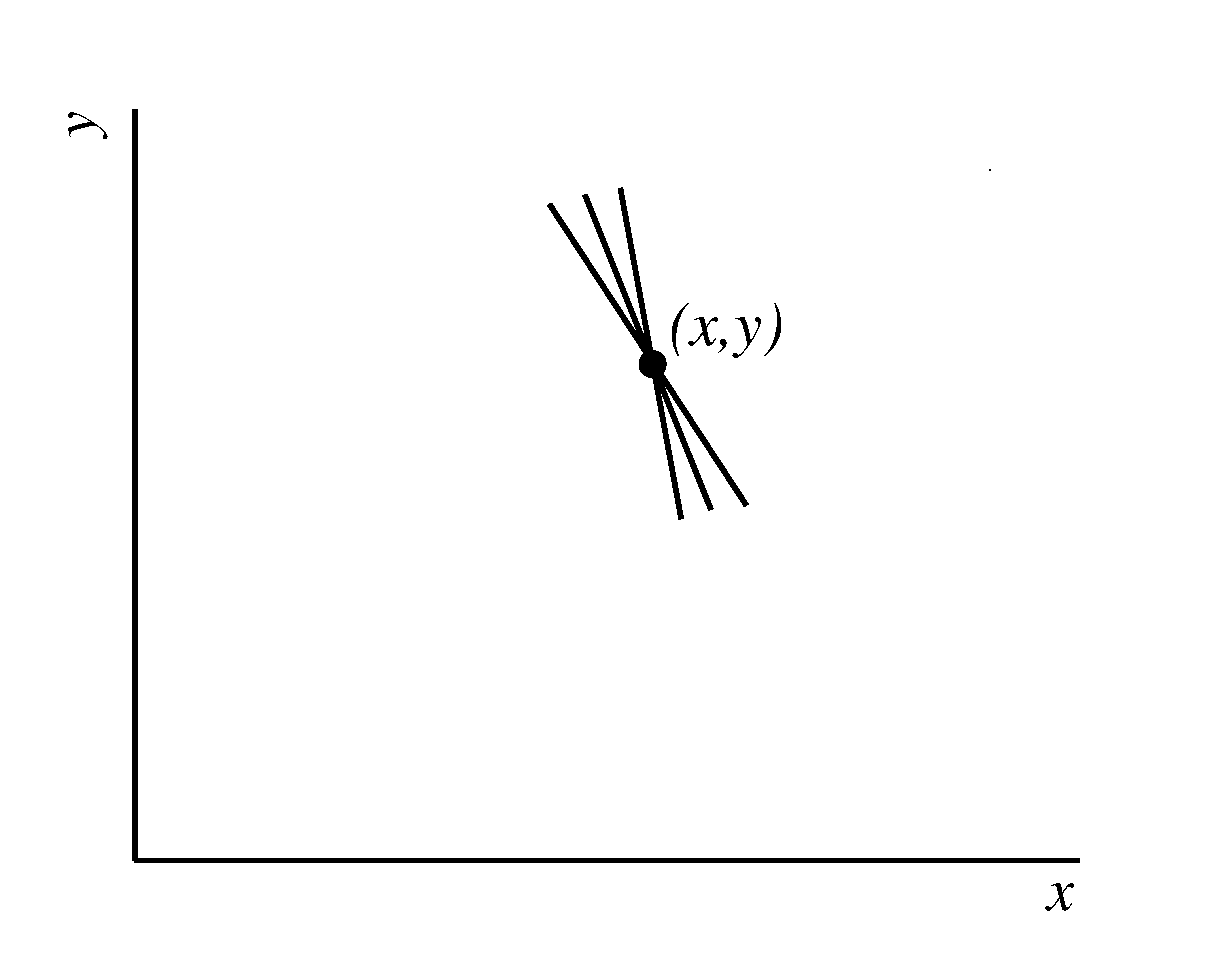
\includegraphics[width=7cm]{images/hough_transform/cartesian_point} \label{fig:2DCartesianPoint}}
  \subfloat[Line in 2D parameter space.]{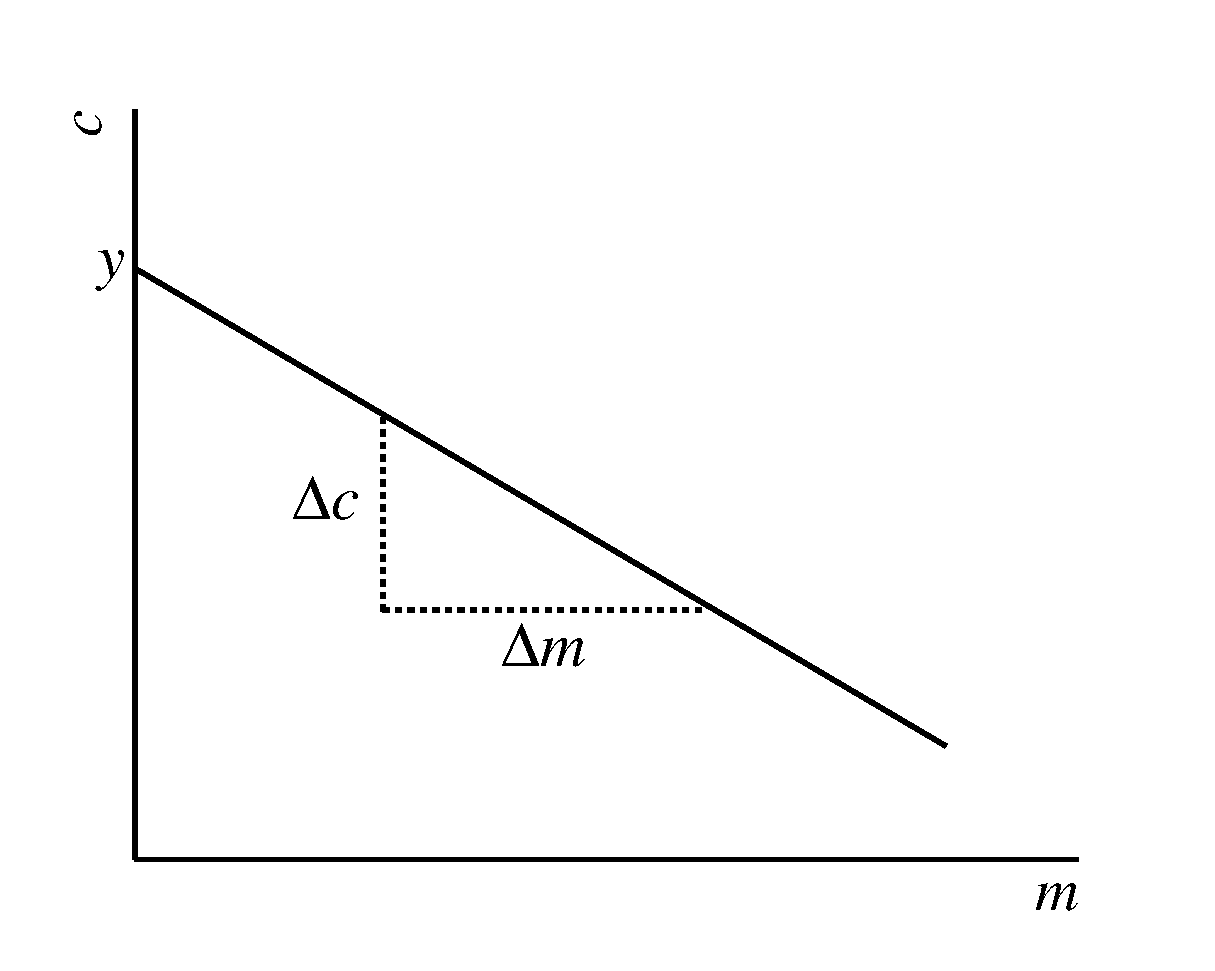
\includegraphics[width=7cm]{images/hough_transform/parameter_line} \label{fig:2DParameterLine}}
  \caption{Representations of a 2D point in cartesian space.}
  \label{fig:2DCartesianPointAndParameterLine}
\end{figure}


\subsection{The parameter space}
\label{subsec:ParameterSpace}
As section~\ref{subsec:LinePointDuality} shows, there is a clear relationship between the cartesian space and the parameter space.  Specifically, there is a symmetry between lines and points contained in the two spaces.  This relationship between the cartesian and parameter spaces is not only interesting but also very powerful.  Consider again the parameter line defined by equation~\ref{eq:2DLineParameter} and shown in Fig.~\ref{fig:2DParameterLine}.  As shown in section~\ref{subsec:LinePointDuality}, equation~\ref{eq:2DLineParameter} was derived by considering the infinite set of lines which pass through a cartesian point.  As this infinite set represents the parameter line, it must also be true that the parameter line represents the infinite line set.  Using one of the results from section~\ref{subsec:LinePointDuality}, any point along the parameter line represents one of the lines from our infinite set.  This key feature of the parameter space is the central component of the Hough transform.  
\newline
\newline
We will now return to the cartesian space for an example of how the Hough transform works.  Let's define three points in this space,
\begin{equation}
  \begin{split}
    &\quad p_{1}: (2,6) \\
    &\quad p_{2}: (4,8) \\
    &\quad p_{3}: (6,10).
  \end{split}
  \label{eq:HTExampleCartesianPoints}
\end{equation}
%\begin{figure}
%  \centering
%  \parbox{7cm}{
%    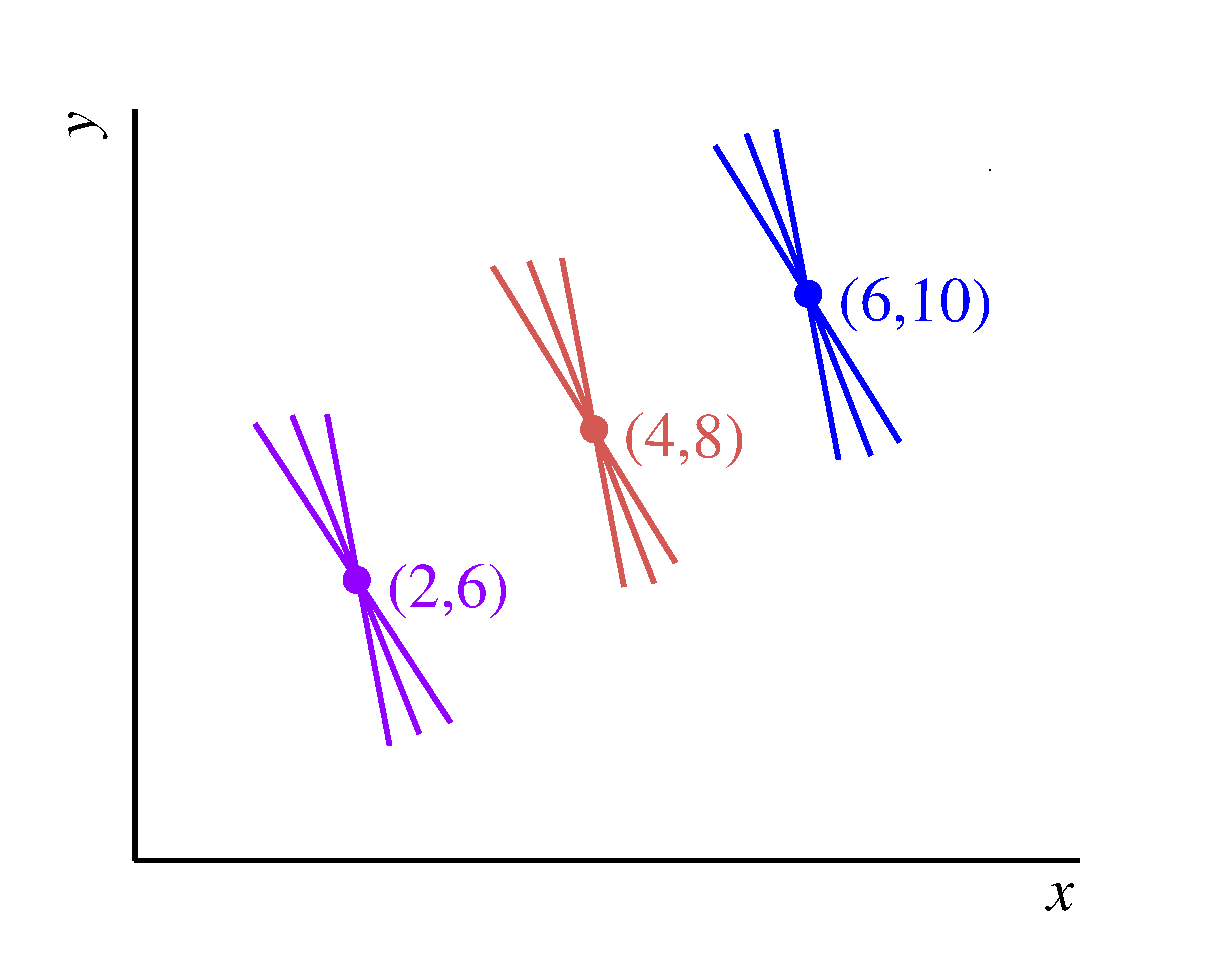
\includegraphics[width=7cm]{images/hough_transform/HT_example_cartesian_space}
%    \caption{The three cartesian points defined in equation~\ref{eq:HTExampleCartesianPoints}.  The colour coding matches that of Fig.~\ref{fig:HTExampleParameterSpace}.}
%    \label{fig:HTExampleCartesianSpace}}
%    \qquad
%    \begin{minipage}{7cm}
%      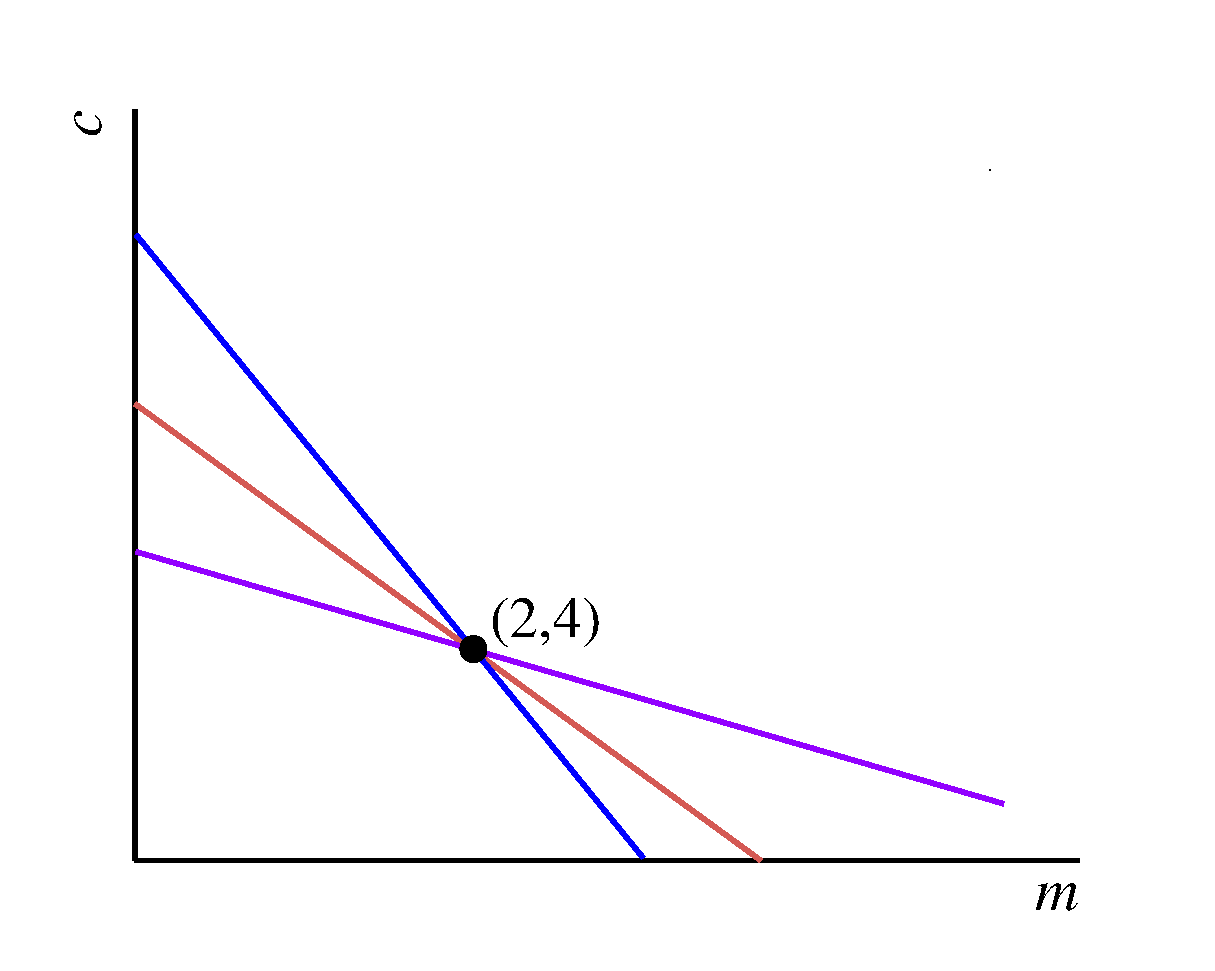
\includegraphics[width=7cm]{images/hough_transform/HT_example_parameter_space}
%      \caption{The three parameter lines defined in equation~\ref{eq:HTExampleParameterLines}.  The same colour coding as Fig.~\ref{fig:HTExampleCartesianSpace} is used.}
%      \label{fig:HTExampleParameterSpace}
%    \end{minipage}
%\end{figure}
\begin{figure}%
  \centering
  \subfloat[The three cartesian points defined in equation~\ref{eq:HTExampleCartesianPoints}.]{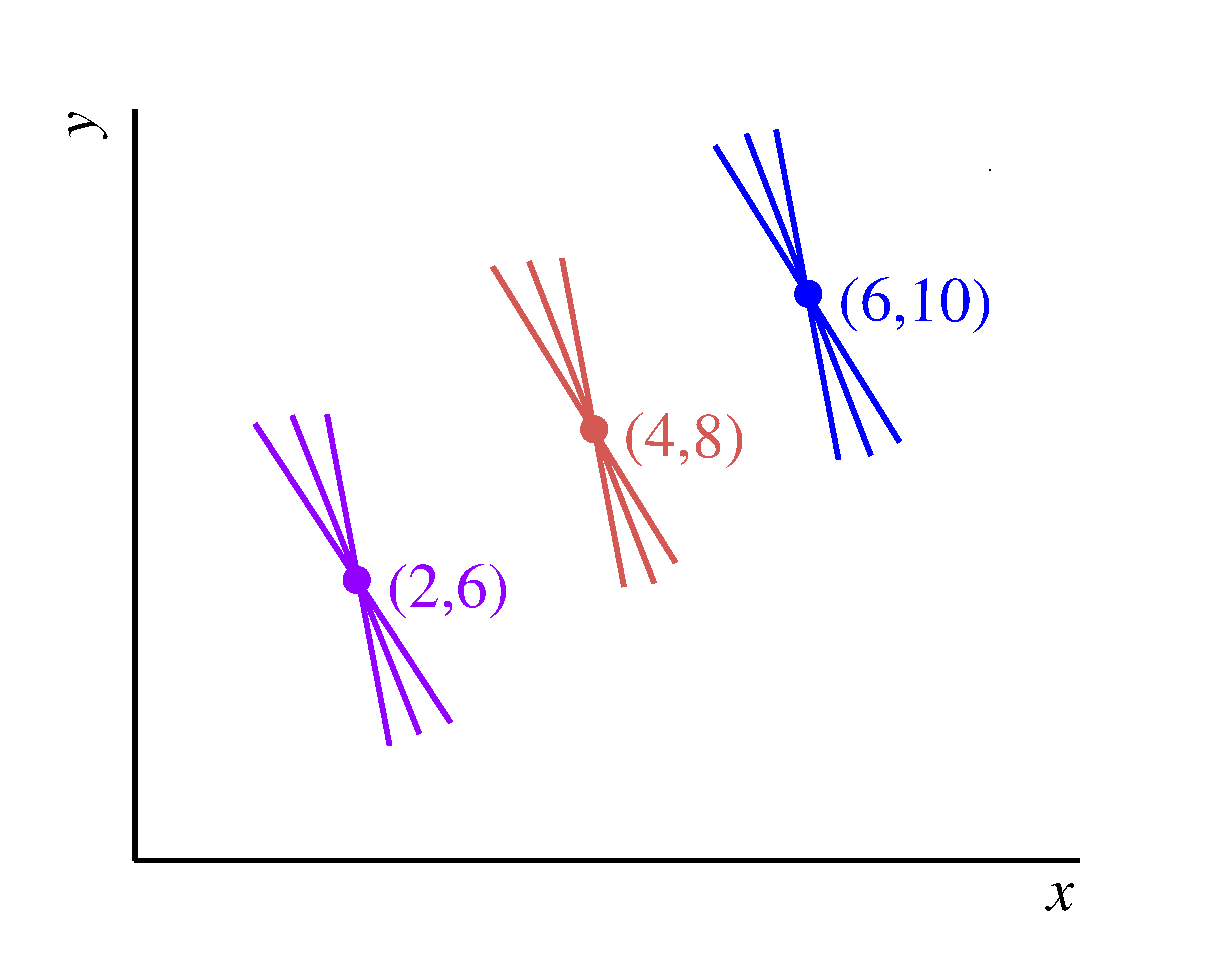
\includegraphics[width=7cm]{images/hough_transform/HT_example_cartesian_space} \label{fig:HTExampleCartesianSpace}}
  \subfloat[The three parameter lines defined in equation~\ref{eq:HTExampleParameterLines}.  The coordinates (2,4) define the point of intersection of the three lines.]{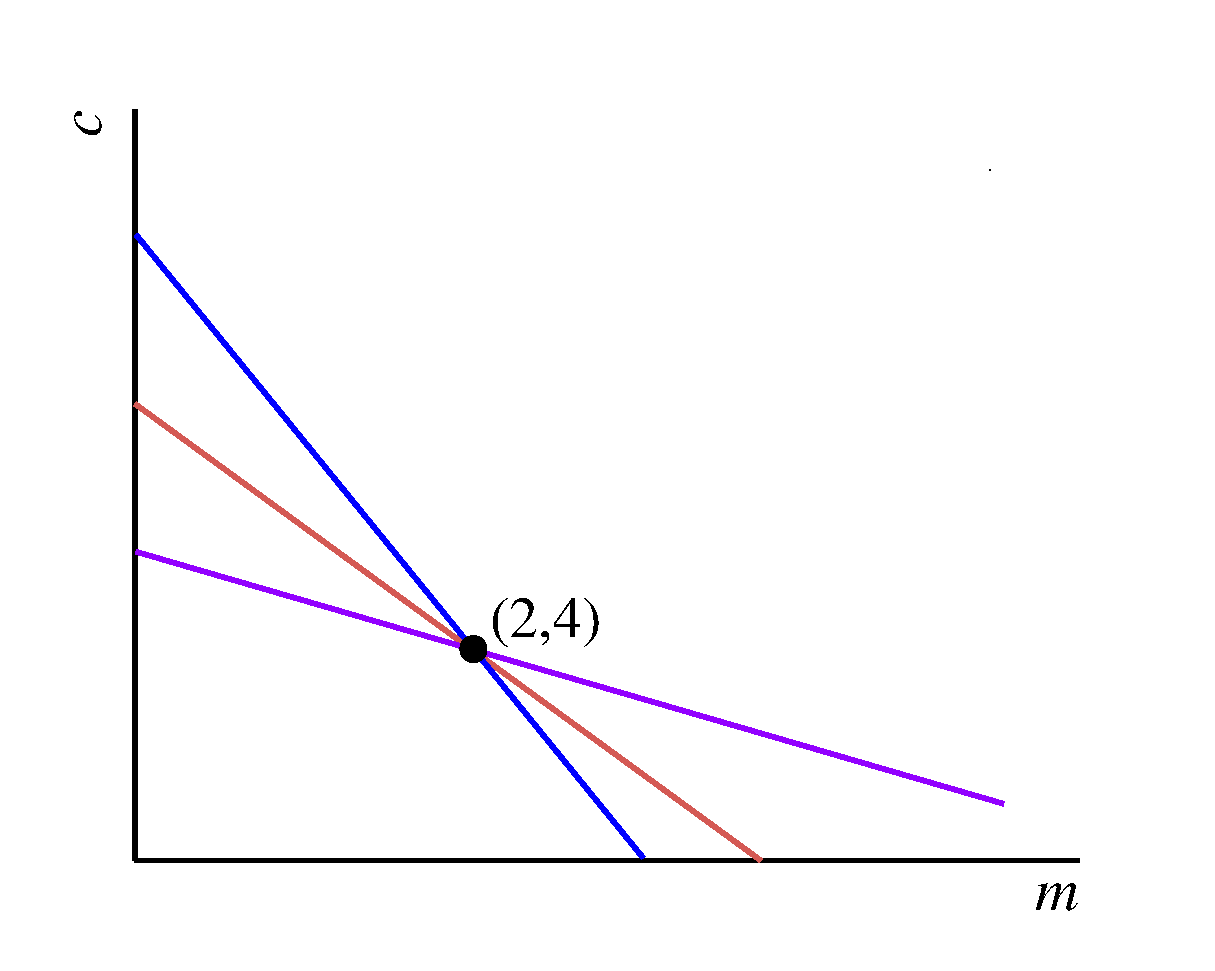
\includegraphics[width=7cm]{images/hough_transform/HT_example_parameter_space} \label{fig:HTExampleParameterSpace}}
  \caption{The three points defined in equation~\ref{eq:HTExampleCartesianPoints} and their representation in the parameter space.  The colour coding matches the cartesian points to their respective parameter lines.}
  \label{fig:HTExample}
\end{figure}
\newline
\newline
The three points defined in equation~\ref{eq:HTExampleCartesianPoints} are shown in Fig.~\ref{fig:HTExampleCartesianSpace}.  Using one of the results from section~\ref{subsec:LinePointDuality} and equation~\ref{eq:2DLineParameter}, the three points can be Hough transformed into the following parameter lines:
\begin{equation}
  \begin{split}
    &\quad c = -2m + 6 \\
    &\quad c = -4m + 8 \\
    &\quad c = -6m + 10.
  \end{split}
  \label{eq:HTExampleParameterLines}
\end{equation}
The three parameter lines are shown in Fig.~\ref{fig:HTExampleParameterSpace}.  From Fig.~\ref{fig:HTExampleParameterSpace}, it is clear that the three parameter lines all cross at a common point with parameter space coordinates (2,4).  Using the results from section~\ref{subsec:LinePointDuality}, this common point in parameter space is represented by a line in cartesian space.  In addition, as (2,4) is common to all three parameter lines, the cartesian line represented by (2,4) must also pass through all three cartesian points defined by equation ~\ref{eq:HTExampleCartesianPoints}.  This new cartesian line is defined by
\begin{equation}
  y = 2x + 4
  \label{eq:HTExampleCartesianLine}
\end{equation}
and is shown in Fig.~\ref{fig:HTExampleCartesianSpaceWithLine} with the original points used to generate the parameter lines.  While this example is relatively simple, it demonstrates the capability of the Hough transform to recognise linear patterns in sets of points.

\begin{figure}
  \centering
  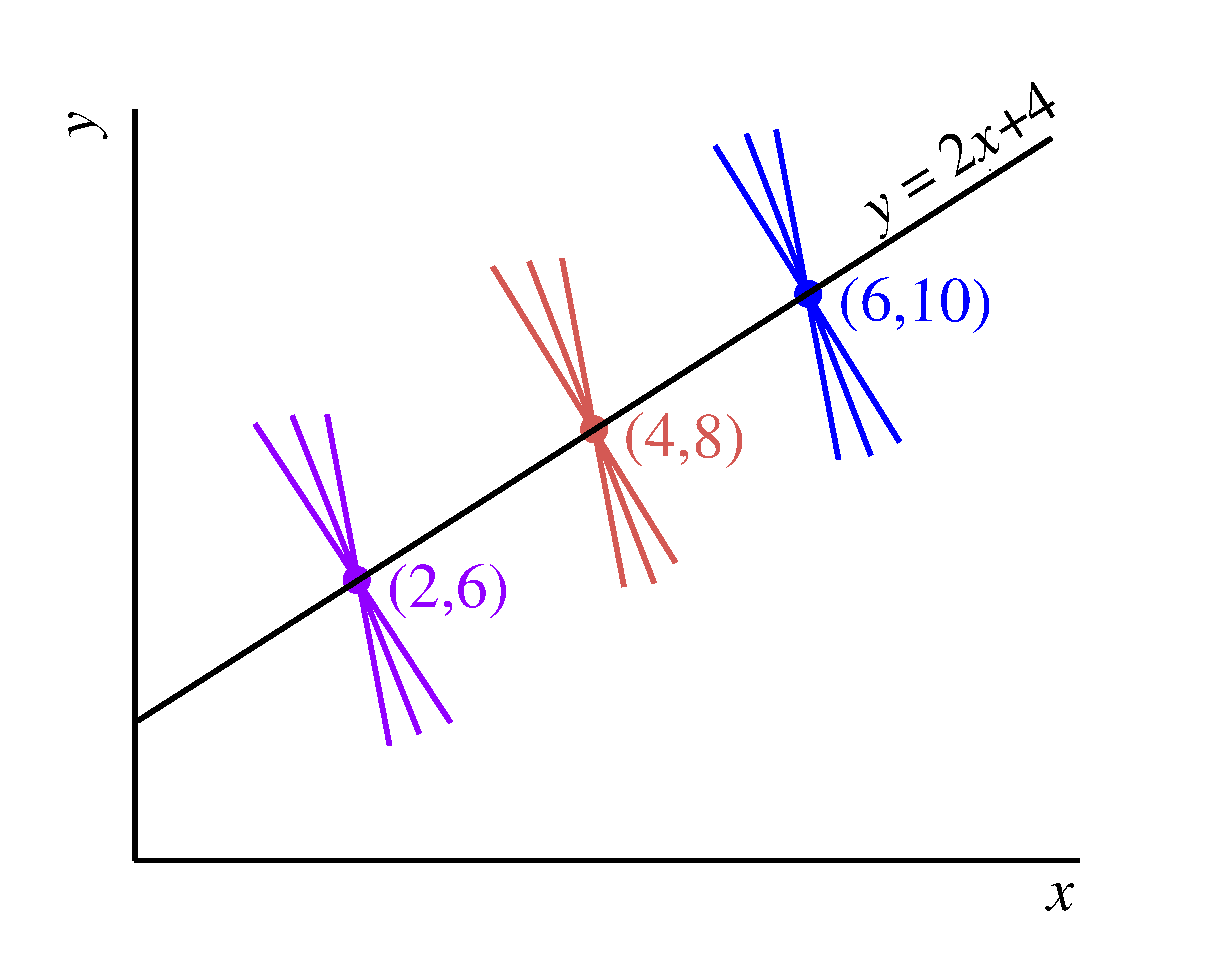
\includegraphics[width=9cm]{images/hough_transform/HT_example_cartesian_space_with_line}
  \caption{The line represented by the intersection in Fig.~\ref{fig:HTExampleParameterSpace} with the cartesian points it intercepts.}
  \label{fig:HTExampleCartesianSpaceWithLine}
\end{figure}

\subsection{Redefinition of parameters}
\label{subsec:ParameterRedefinition}
Unfortunately, a complication in computation arises when $m\rightarrow\infty$.  However, this complication can be removed by redefining the line parameters such that one is bounded.  An alternative 2D line parameterisation is to specify a line in terms of the angle it makes with the $x$ axis, $\theta$, and the perpendicular distance of the line from the origin, $\rho$, as illustrated in Fig.~\ref{fig:CartesianParameterRedefinition}.  The functional form of the cartesian line becomes 
\begin{equation}
  y = x\textrm{tan}\theta + \frac{\rho}{\textrm{cos}\theta}.
  \label{eq:CartesianLineReparameterisation}
\end{equation}
Using this new parameterisation, we must also define a new parameter space with axes $\theta$ and $\rho$.  Using equation~\ref{eq:CartesianLineReparameterisation}, a line in this new parameter space is defined by
\begin{equation}
  \rho = y\textrm{cos}\theta - x\textrm{sin}\theta.
  \label{eq:ParameterLineReparameterisation}
\end{equation}
By definition, the $\theta$ axis of the parameter space must be bounded to the interval [0,2$\pi$].  If the directionality of the line is meaningless to the analyser, then the interval can be restricted to [0,$\textrm{\pi}$].
\newline
\newline
The disadvantage of this parameterisation is that parameter line generation now involves trigonometric calculations which can be computationally expensive.  However, this problem is small when compared to the unbounded complication of the traditional parameterisation.

\begin{figure}
  \centering
  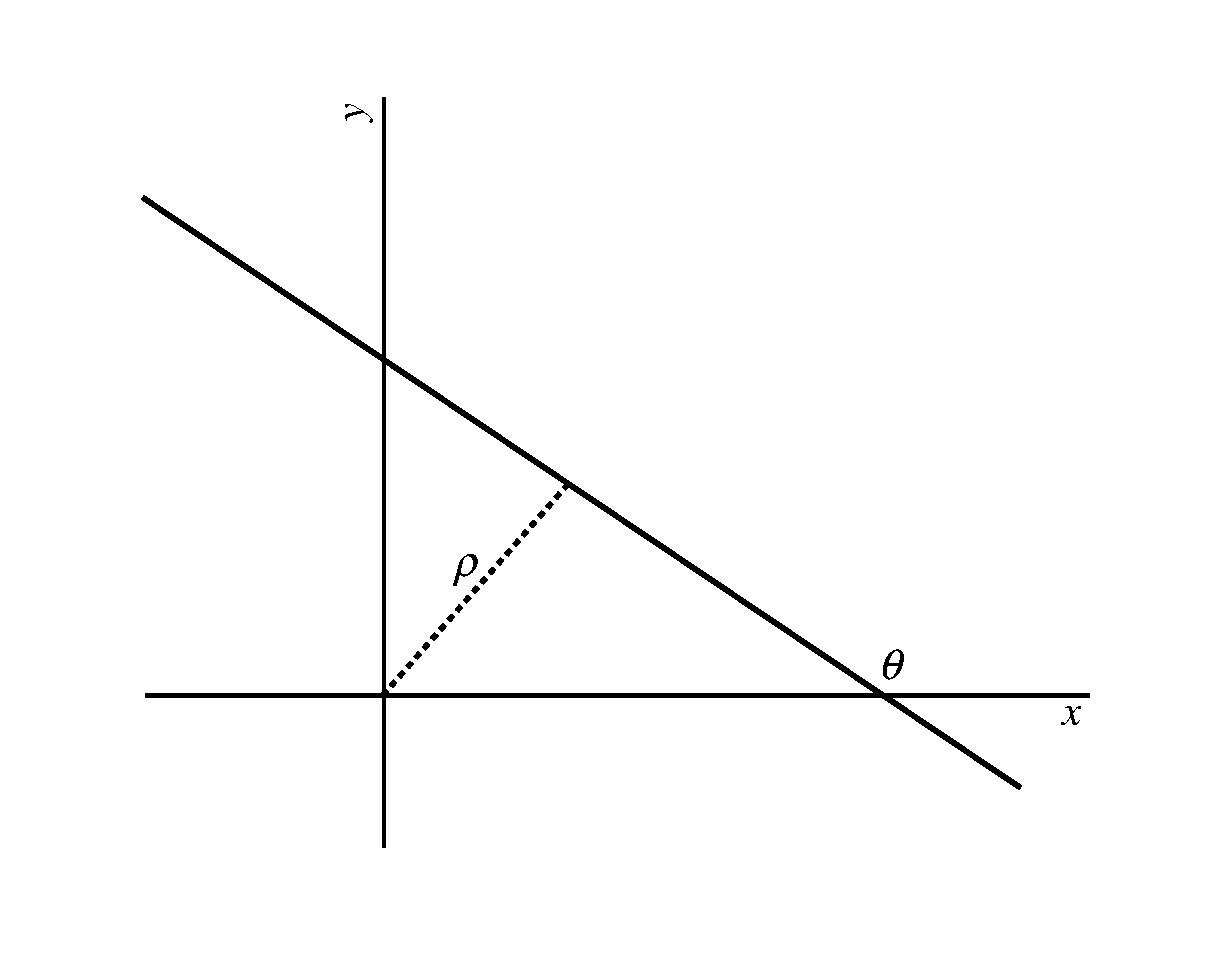
\includegraphics[width=9cm]{images/hough_transform/cartesian_parameter_redefinition}
  \caption{$\theta-\rho$ parameterisation of a 2D line.}
  \label{fig:CartesianParameterRedefinition}
\end{figure}



\subsection{Discretisation of the parameter space}
\label{subsec:ParameterSpaceDiscretisation}
It must now be considered how the parameter space is analysed.  When a large number of parameter lines are generated, it becomes computationally expensive to analyse the resultant parameter space.  While approaches exist to analyse the parameter space with very high precision~\cite{331821}, it is often only necessary to extract parameters with finite resolution.  In such a case, it is convenient to discretise the parameter space.  Under this regime, the parameter space is split into $\theta-\rho$ bins.  Then, a parameter line is generated by incrementing the value of each $\theta-\rho$ bin it passes through.  After each line has been added to the parameter space, the crossing locations can be readily found by searching for the $\theta-\rho$ bins with content larger than unity.  An example of this discretisation is illustrated in Fig.~\ref{fig:BinnedParameterSpace}, where the parameter lines defined in equation~\ref{eq:HTExampleParameterLines} have been re-parameterised using equation~\ref{eq:ParameterLineReparameterisation}.  The content of each bin in Fig.~\ref{fig:BinnedParameterSpace} records how many of the three parameter lines pass through each bin.  The bin with value 3 is the crossing point of the three parameter lines.
\newline
\newline
If a discretised approach is acceptable, which is the case in event reconstruction, construction and analysis of the parameter space is reduced to filling a 1D array $N$ times, where $N$ is the number of parameter lines, followed by a 1D grid search of the array to find the bin with the highest content.
\begin{figure}
  \centering
  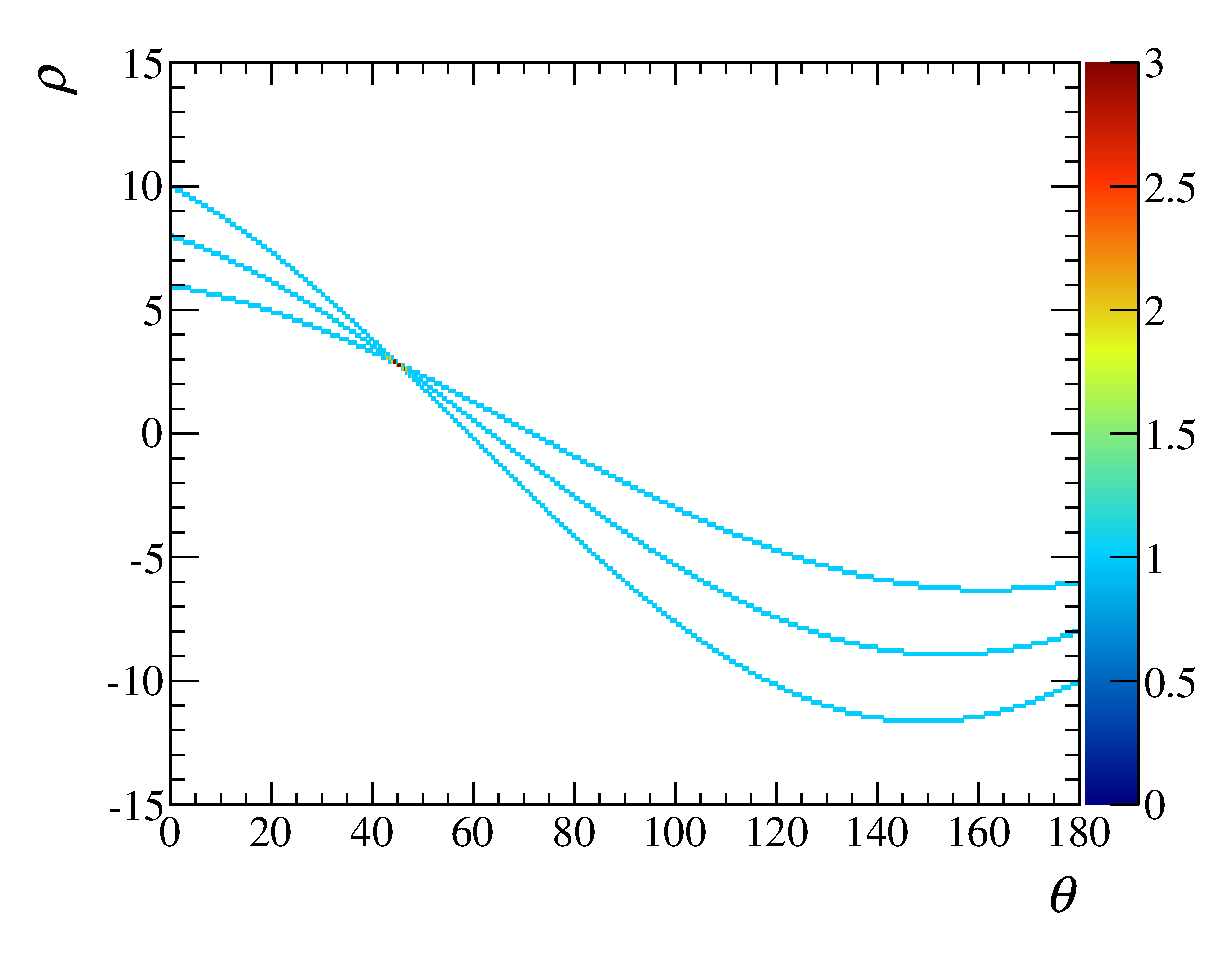
\includegraphics[width=9cm]{images/hough_transform/binned_parameter_space}
  \caption{The discrete $\theta-\rho$ space.  The plotted lines are those defined in equation~\ref{eq:HTExampleParameterLines} and reparameterised using equation~\ref{eq:ParameterLineReparameterisation}.}
  \label{fig:BinnedParameterSpace}
\end{figure}



\section{ECal application of the Hough transform}
\label{sec:ECalApplicationHoughTransform}
We must now address how the Hough transform can be used as a reconstruction tool in the ECal.  To do this, let's consider a neutrino interaction which occurs in the ECal as illustrated in~\ref{fig:3StateInteractionNoReconstruction}.  While the propagating neutrino is invisible to the ECal, the charged final state are definitely not.  To first order, the final state particles propagate in straight lines depositing energy in the scintillator bars as they go.  From this, we can infer that the hit bars arranged in straight lines should reveal the trajectory of the final states.  As shown above, the Hough transform is capable of identifying straight lines from a set of coordinates.  However, there are two complications in the ECal which the above sections have not addressed.  We have only specifically discussed how to extract a single straight line from a pattern.  As Fig.~\ref{fig:3StateInteractionNoReconstruction} shows, the number of final states can be, and is often, greater than one.  This is merely a problem of computation which will be addressed in section~\ref{subsec:ParameterSpaceAnalysis}.  A much more severe problem is that the above demonstrations only deal with patterns constructed from infinitesimal points.  While the centre of a scintillator bar can be used as a point for parameter line generation, it is unlikely that a final state particle will pass through the central point of the scintillator bars that it propagates through.  If this is not addressed, the Hough transform will be of little use in trajectory reconstruction.
\begin{figure}
  \centering
  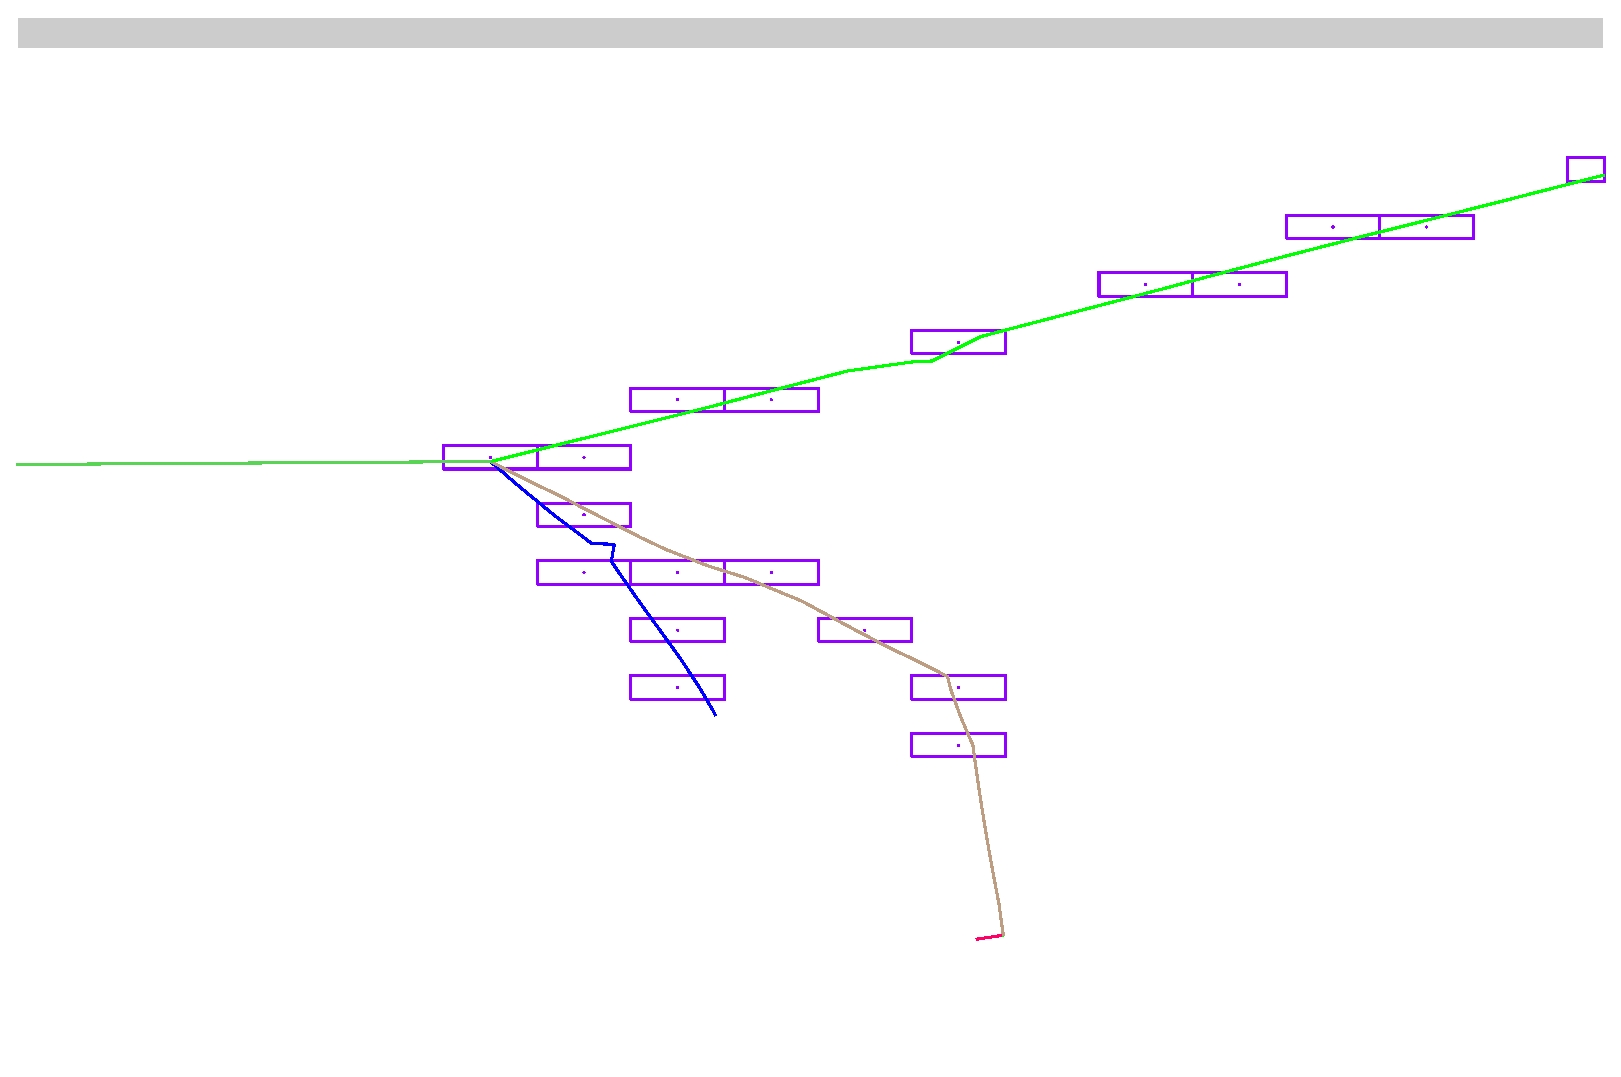
\includegraphics[width=10cm]{images/hough_transform/3StateInteraction_SideLeftECal_NoReconstruction.eps}
  \caption{Simulated neutrino interaction with 3 final states in the side-right ECal.  The green line entering from the left is the $\nu_\mu$.  The green line exiting to the right is a $\mu^{-}$, the brown line is a $\pi^+$ and the blue line is a proton.  The purple rectangles represent the hit ECal bars.}
  \label{fig:3StateInteractionNoReconstruction}
\end{figure}

\subsection{Modelling the ECal bar}
\label{subsec:ECalBarModel}
To make the Hough transform viable as a reconstruction tool, the finite dimensions of the ECal bar need to be incorporated into the parameter space generation.  This feature of the ECal bars would be very problematic if the parameter space was continous.  However, it is only necessary to know the line parameters with finite resolution and a discrete parameter space can be used.  This means that the ECal bar can be modelled as a set of cartesian points and each of said points can be Hough transformed in turn to build up the parameter line representation of the ECal bar.
\newline
\newline
There are now two steps to consider.  Firstly, how should the points be arranged?  Remember that the Hough transform of a point represents all of the lines that pass through that point.  So, the points should be arranged in such a fashion that any line which passes through the 2D cross-section of the ECal bar also has to pass through one of the points in the configuration.  Secondly, the spacings between the points should be small enough that no gaps appear in the generated parameter line.  
\newline
\newline
Assuming that every bin of the parameter space will have a 1$^\circ\times$1 mm area, an obvious choice would be to use a rectangular grid of points with 1 mm spacing superimposed over the 2D cross-section of an ECal bar.  The total number of points used to model the ECal bar is 451.  To Hough transform the ECal bar, every point in the grid array can be Hough transformed individually with care taken to ensure that each $\theta-\rho$ bin is filled exactly once.  The result is illustrated in Fig.~\ref{fig:ECalBarHoughTransformGridRepresentation}.  The finite size of the ECal bar is evident by the finite size of the resultant parameter line.
%\begin{figure}
%  \centering
%  \parbox{7cm}{
%    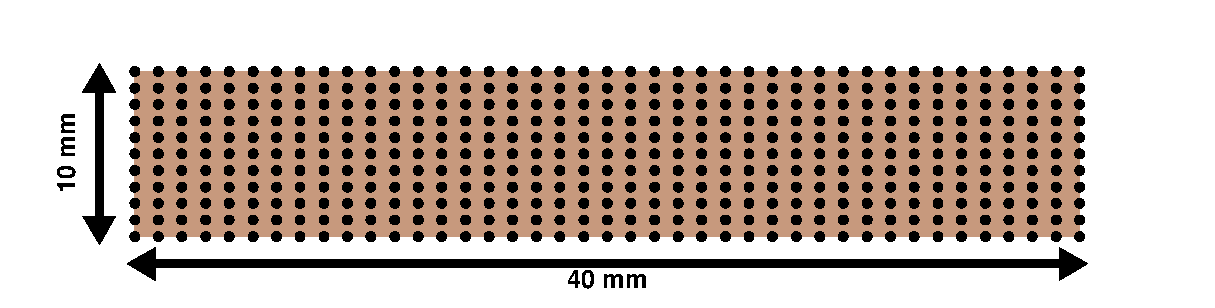
\includegraphics[width=7cm]{images/ecal_hough_transform/ecal_grid_array.eps}
%    \caption{Grid representation of an ECal bar.}
%    \label{fig:ECalBarGridRepresentation}}
%    \qquad
%    \begin{minipage}{7cm}
%      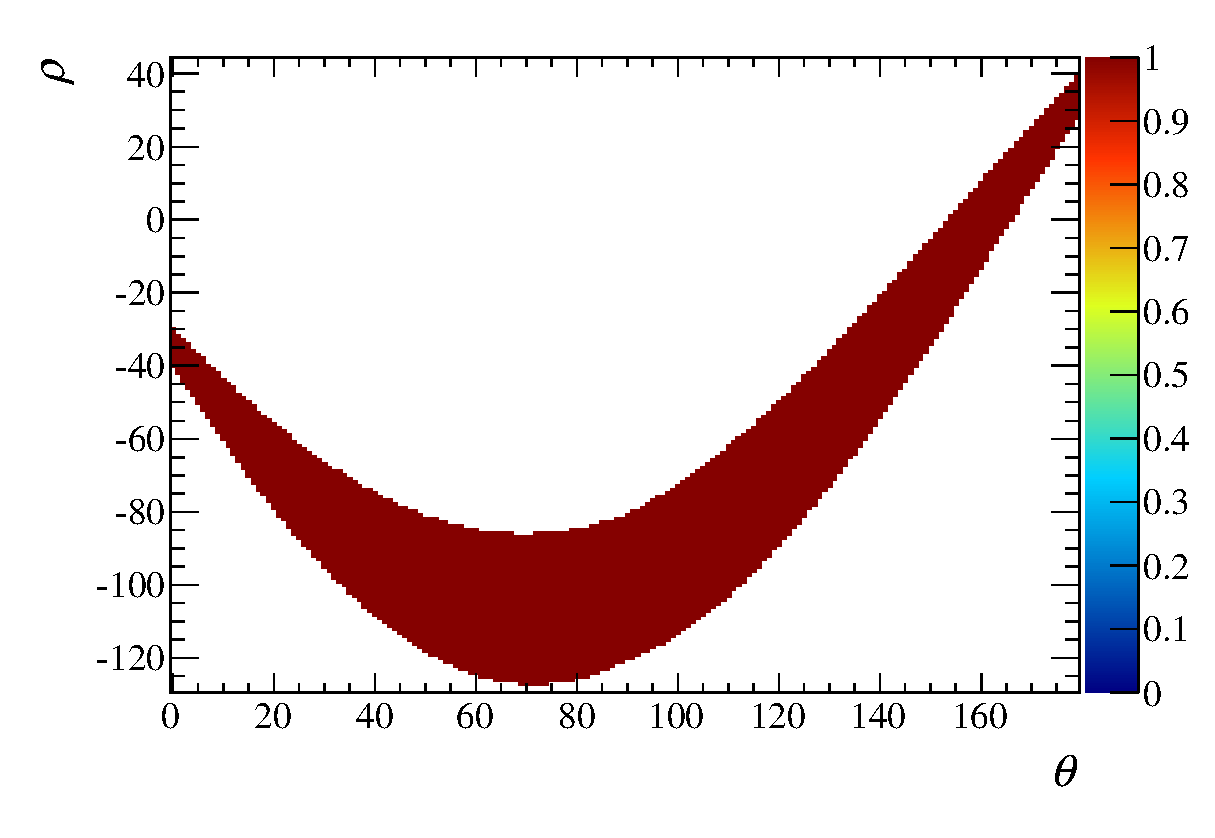
\includegraphics[width=7cm]{images/ecal_hough_transform/single_ecal_bar_hough_transform.eps}
%      \caption{Single ECal bar Hough transform using the point configuration shown in Fig.~\ref{fig:ECalBarGridRepresentation}.}
%      \label{fig:ECalBarHoughTransformGridRepresentation}
%    \end{minipage}
%\end{figure}
\begin{figure}%
  \centering
  \subfloat[Grid representation of an ECal bar.]{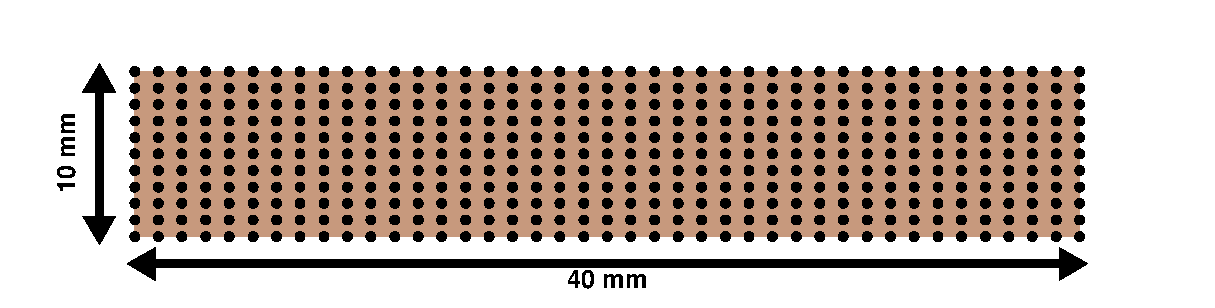
\includegraphics[width=7cm]{images/ecal_hough_transform/ecal_grid_array.eps} \label{fig:ECalBarGridRepresentation}}
  \subfloat[Single ECal bar Hough transform using the point configuration shown in Fig.~\ref{fig:ECalBarGridRepresentation}.]{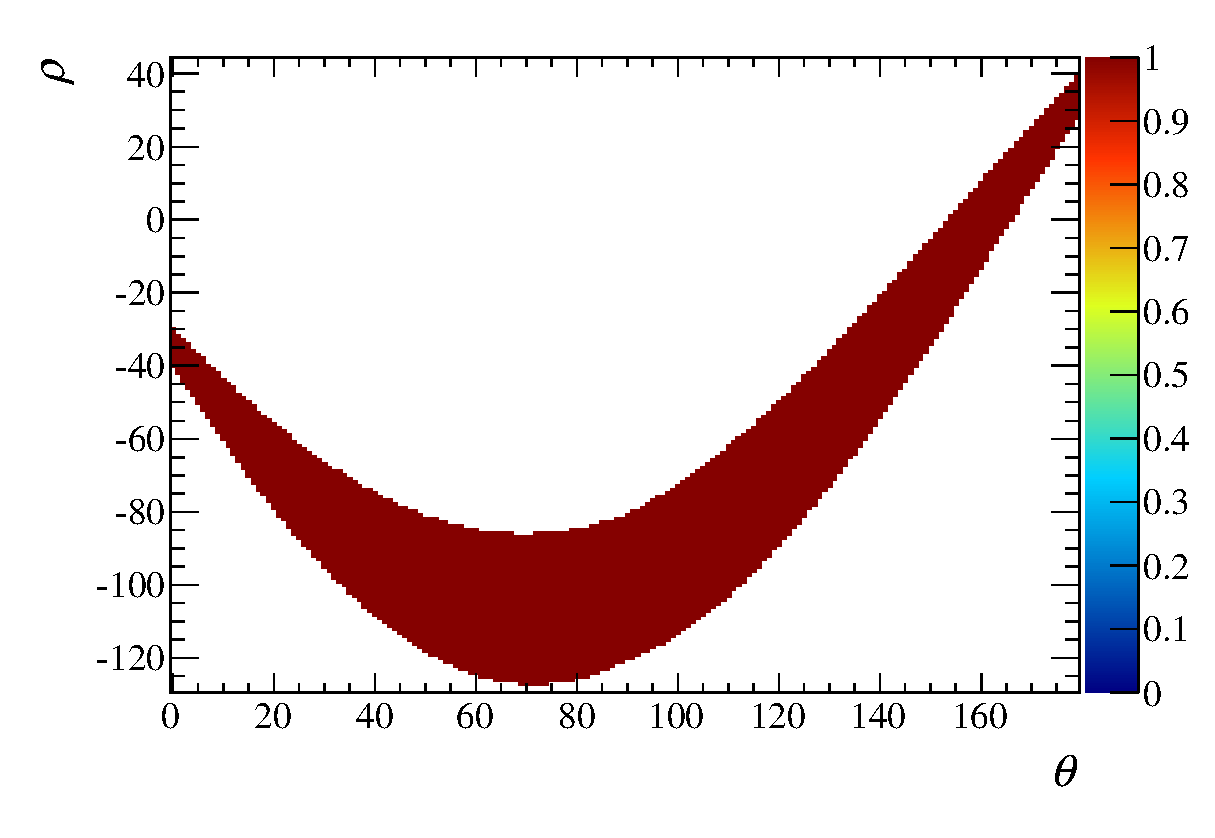
\includegraphics[width=7cm]{images/ecal_hough_transform/single_ecal_bar_hough_transform.eps} \label{fig:ECalBarHoughTransformGridRepresentation}}
  \caption{The grid representation of an ECal bar and its representation in parameter space.}
  \label{fig:ECalBarGridRepresentationAndHoughTransform}
\end{figure}
\newline
\newline
While the generated parameter line accurately represents every line which passes through the ECal bar, there are two problems with this approach.  Firstly, the large number of points to be Hough transformed is very large which results in a long CPU time.  Secondly, there is a very high number of redundant calculations involved in the parameter line generation.  Consider an exactly vertical line which passes through one of the points in the grid array.  This line also passes through 10 other points in the same column of the grid.  This means that when the parameter line is being generated, this vertical line is calculated 11 times for each column.  Bearing this in mind, there are many points along the parameter line which are repeatedly calculated and provide no extra information.  This would mean that any algorithm which uses this approach would be very CPU inefficient.
\newline
\newline
An alternative is to model the ECal bar as a set of points arranged in a cross as shown in Fig.~\ref{fig:ECalBarCrossRepresentation}.  Assuming that the spacing between the points on each line of the cross is infinitesimal, any line which passes through the ECal bar would also have to pass through one of the points in the configuration.  As the parameter space is discrete, the spacing between the points need not be infinitesimal but only small enough to ensure that no gaps appear in the parameter line.  Using 45 points on each line of the cross, the ECal bar can be Hough transformed by Hough transforming each point in the cross configuration. An example of this result is shown in Fig.~\ref{fig:ECalBarHoughTransformCrossRepresentation} using the same ECal bar used to generate Fig.~\ref{fig:ECalBarHoughTransformGridRepresentation}.  Clearly, Fig.~\ref{fig:ECalBarHoughTransformGridRepresentation} and Fig.~\ref{fig:ECalBarHoughTransformCrossRepresentation} are identical showing that the cross model achieves the same result as the grid model.  Comparing the two, the cross model uses a 90 point representation whereas the grid model uses a 451 point representation.  This should mean that an algorithm utilising the cross model would be a factor of five faster than one using a grid model.
\begin{figure}%
  \centering
  \subfloat[Cross representation of an ECal bar.]{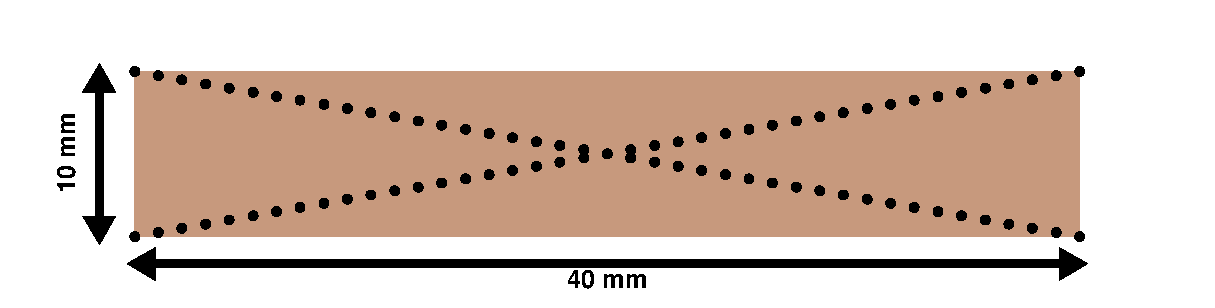
\includegraphics[width=7cm]{images/ecal_hough_transform/ecal_cross_array.eps} \label{fig:ECalBarCrossRepresentation}}
  \subfloat[Single ECal bar Hough transform using the point configuration shown in Fig.~\ref{fig:ECalBarCrossRepresentation}.]{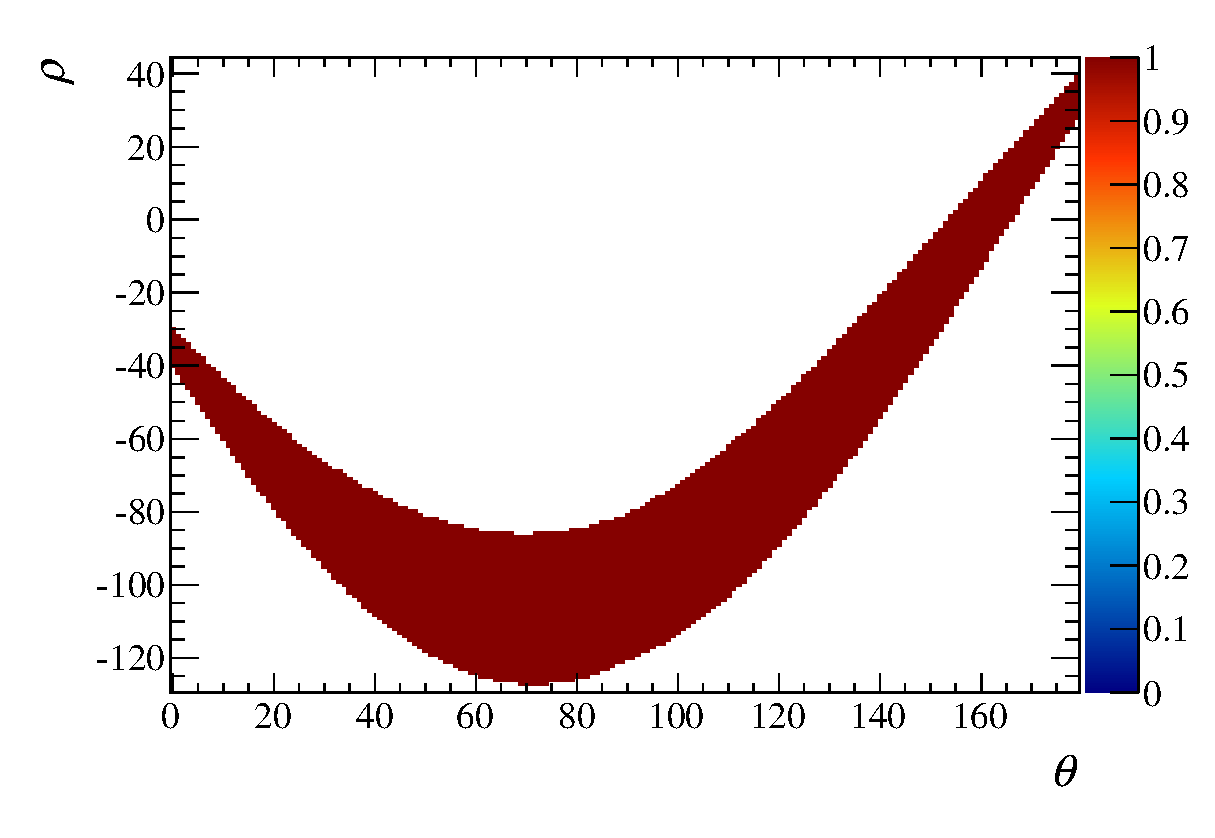
\includegraphics[width=7cm]{images/ecal_hough_transform/single_ecal_bar_hough_transform.eps} \label{fig:ECalBarHoughTransformCrossRepresentation}}
  \caption{The cross representation of an ECal bar and its representation in parameter space.}
  \label{fig:ECalBarCrossRepresentationAndHoughTransform}
\end{figure}
%\begin{figure}
%  \centering
%  \parbox{7cm}{
%    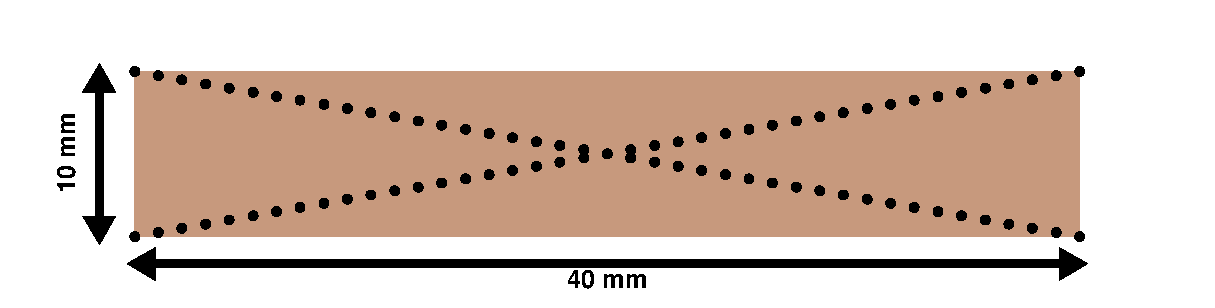
\includegraphics[width=7cm]{images/ecal_hough_transform/ecal_cross_array.eps}
%    \caption{Cross representation of an ECal bar.}
%    \label{fig:ECalBarCrossRepresentation}}
%    \qquad
%    \begin{minipage}{7cm}
%      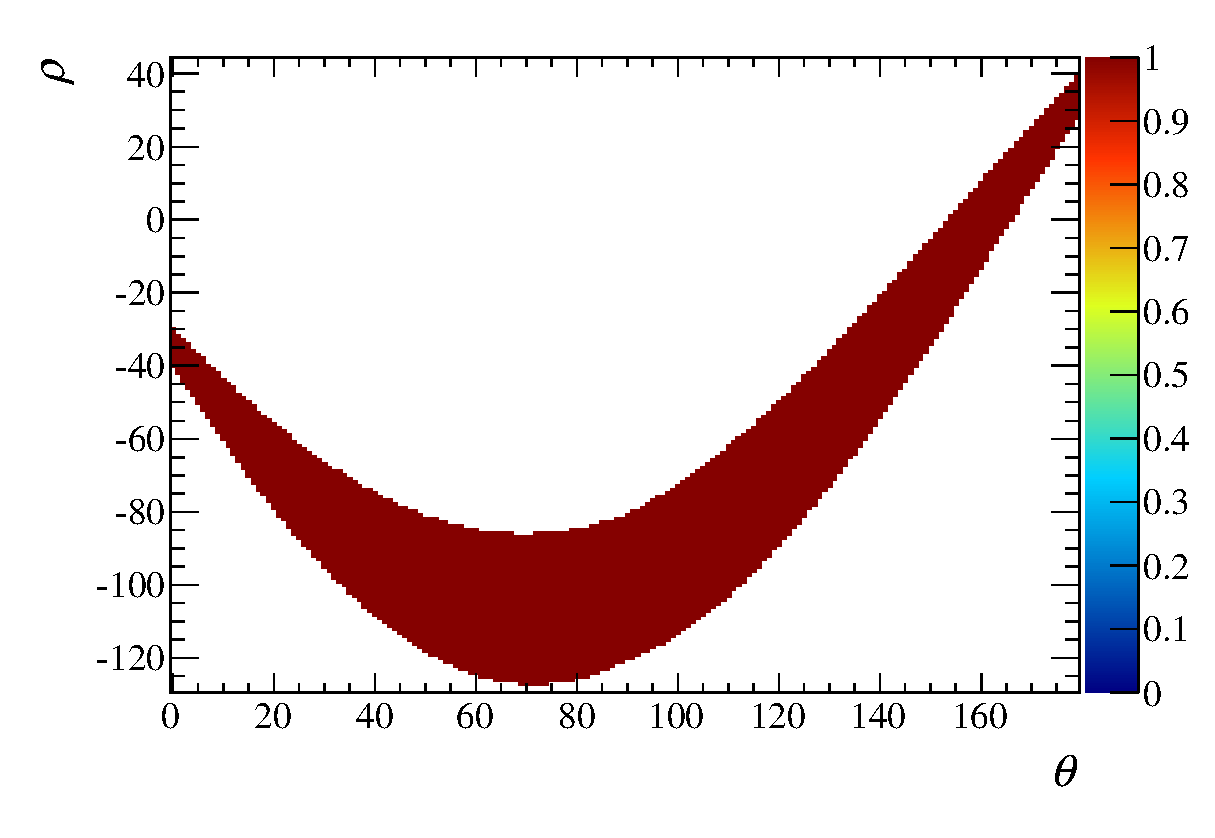
\includegraphics[width=7cm]{images/ecal_hough_transform/single_ecal_bar_hough_transform.eps}
%      \caption{Single ECal bar Hough transform using the point configuration shown in Fig.~\ref{fig:ECalBarCrossRepresentation}.}
%      \label{fig:ECalBarHoughTransformCrossRepresentation}
%    \end{minipage}
%\end{figure}
%\subsection{ECal bar Hough transform}
%\label{subsec:ECalBarHoughTransform}
%Hough transform the points on the cross

\subsection{Parameter space generation}
\label{subsec:ParameterSpaceGeneration}
As we have addressed how to Hough transform an ECal bar, we are now in suitable position to generate the full parameter space for an ECal cluster.  As described in section~\ref{subsec:ParameterRedefinition}, the parameterisation of the 2D lines requires some point in space to act as the origin.  It is possible to use the origin defined by the global ND280 geometry, however this is located in TPC 1 which would mean $\rho$ will usually be the order of metres.  It is more convenient to define an origin in the vicinity of the ECal cluster being reconstructed.  A simple option is to use the charge-weighted centre of the ECal cluster as the origin of the Hough transform.  This location is simple to calculate and generally keeps $\rho$ small.
\newline
\newline
The provided description of the Hough transform in all previous sections is strictly defined in 2D and so the ECal cluster should be split in such a way that this definition can be used.  Fortunately, a 3D ECal cluster is built up using the two 2D views that the scintillator layers provide.  So, it is relatively easy to split the 3D cluster into a pair of 2D clusters by collecting the cluster's hits into their respective 2D views.
\newline
\newline
We can now partly answer one of the problems raised in section~\ref{sec:ECalApplicationHoughTransform} which is how to handle the track multiplicity aspect of the reconstruction?  This is partly addressed by generating $N$ parameter spaces with the same $\theta-\rho$ bin configuration where $N$ is the number of hits in the 2D cluster.  Each of the $N$ parameter spaces will hold one parameter line generated by one of the 2D hits (in a similar fashion to Fig.~\ref{fig:ECalBarHoughTransformCrossRepresentation}).  The final parameter space can then be generated by adding together each of the $N$ parameter spaces.  The parameter space of the 2D cluster in Fig~\ref{fig:3StateInteractionNoReconstruction} is shown in Fig.~\ref{fig:FullParameterSpace3StateInteraction}.
\begin{figure}
  \centering
  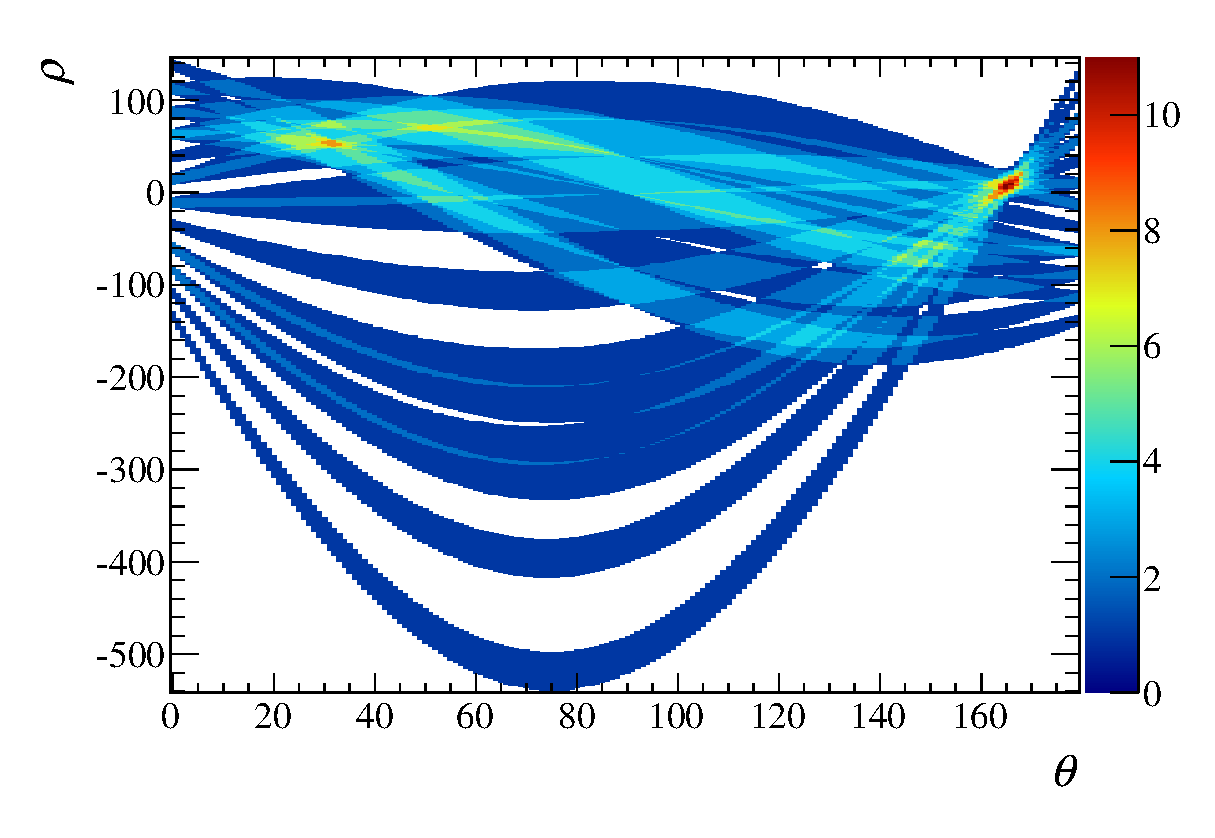
\includegraphics[width=10cm]{images/ecal_hough_transform/FullParameterSpace_3StateInteraction.eps}
  \caption{The full parameter space of the 2D cluster shown in Fig.~\ref{fig:3StateInteractionNoReconstruction}.}
  \label{fig:FullParameterSpace3StateInteraction}
\end{figure}


\subsection{Parameter space analysis}
\label{subsec:ParameterSpaceAnalysis}
The full parameter space can look arbitarily complicated. However, it contains a vast amount of trajectory related information about the cluster.  Every $\theta-\rho$ bin of the parameter space describes a 2D track and the content value of said bin describes how many 2D ECal hits the track passes through.  As described in section~\ref{sec:ECalApplicationHoughTransform}, a particle's trajectory should be straight in the ECal which means that the particles path should be revealed by finding the most hits arranged in a line.  This hit arrangement can be found by finding the bin in the full parameter space with the highest value.  The track candidate parameters can the be found by fetching the ($\theta$,$\rho$) coordinate of the found bin.
\newline
\newline
While the preferred bin can reveal how many hits the track candidate passed through, it contains no information about which hits were contributors.  However, this full parameter space was generated by summing the $N$ parameter spaces discussed in section~\ref{subsec:ParameterSpaceGeneration}.  So, the contributing hits can be readily found by looking at the same ($\theta$,$\rho$) bin in each of the $N$ parameter spaces and recording which have a non-zero value.  We now have the track candidate's parameters and its contributing hits which is enough to describe the 2D trajectory.
\newline
\newline
A new search now needs to begin to find any other track candidates.  However, repeating the same search of the full parameter space will return the track candidate that has already been found.  To find the next track candidate, the presence of the previous track candidate must be removed.  So, a reduced parameter space must be generated. The previous step found which of the $N$ parameter lines contributed to the previous track candidate.  So, this new parameter space can be formed by subtracting the contributing parameter lines from the full space.  An example of this is shown in Fig.~\ref{fig:ReducedParameterSpace3StateInteraction} where the reduced parameter space was formed by subtracting the contributing parameter lines to the highest bin in Fig.~\ref{fig:FullParameterSpace3StateInteraction}.  The next track candidate can then be found by searching for the highest content bin of this reduced parameter space and said bin's contributing parameter lines. 
\newline
\newline
This process can be repeated until some threshold is reached.  This threshold is nominally set by demanding that at least three hits are required to form a track candidate.
\begin{figure}
  \centering
  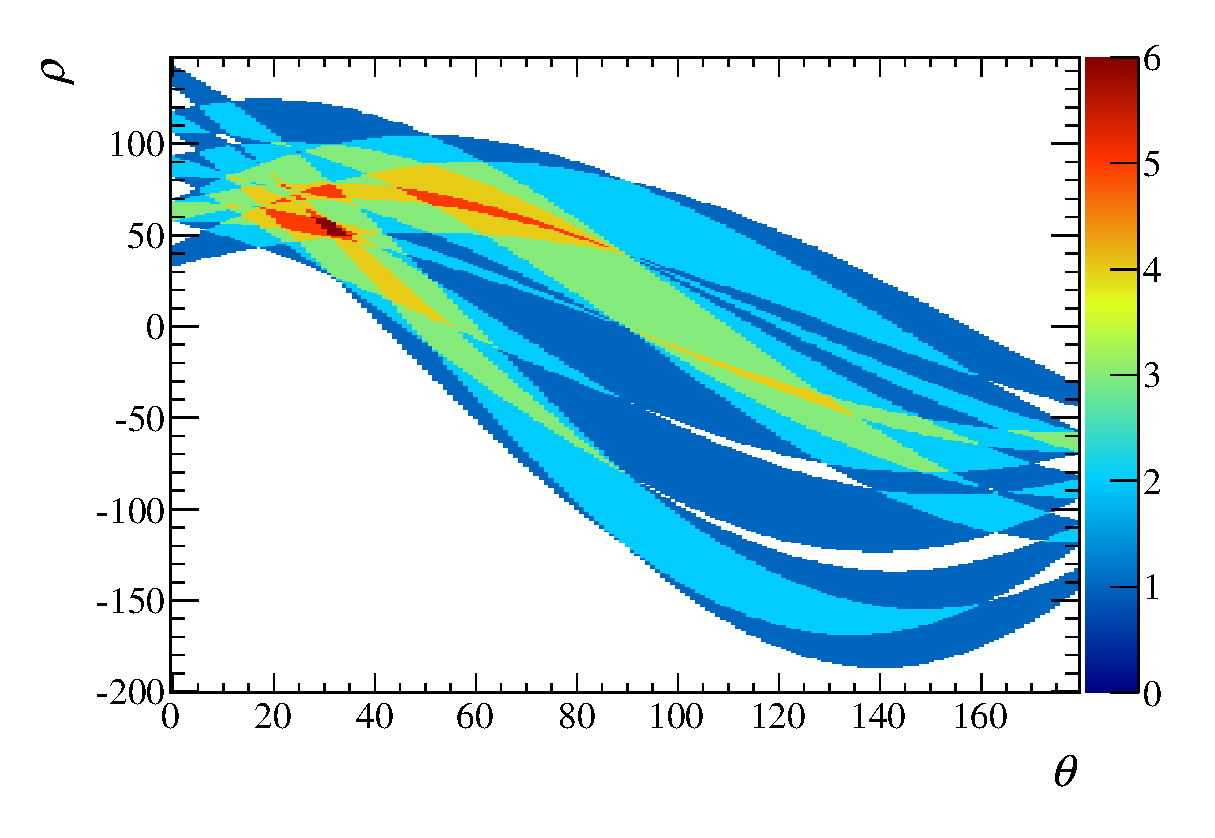
\includegraphics[width=10cm]{images/ecal_hough_transform/ReducedParameterSpace_3StateInteraction.eps}
  \caption{The reduced parameter space of the 2D cluster shown in Fig.~\ref{fig:3StateInteractionNoReconstruction}.}
  \label{fig:ReducedParameterSpace3StateInteraction}
\end{figure}

\subsection{2D track quality checks}
\label{subsec:2DTrackQualityChecks}
While the approach outlined above is very powerful for recognising track-like shapes in the 2D ECal clusters, it is not capable of checking whether the selected track candidates are of sound quality.  So, external checks need to be done which validate each track as it is returned from the parameter space.  Fortunately, the objects returned from parameter space are simple in structure and so the quality checks can be designed to reflect this.  Two necessary checks were implemented in the 2D reconstruction:
\begin{itemize}
\item The track can not skip a scintillator layer in a given view.
\item The track can skip a maximum of 1 bar in a scintillator layer.
\end{itemize}
If a track fails either of the above conditions, the track is flagged as bad and rejected.  To ensure that the same bad track is not selected in the next interation of the parameter space analysis, the track also needs removing from the parameter space.  To do this, every bin in the parameter space is checked to see if the bin is filled purely from the hits contained in the bad track.  If this is the case, the bin content is set to 0.  

\subsection{3D track reconstruction}
\label{subsec:3DHoughTrackReconstruction}
Section~\ref{subsec:ParameterSpaceAnalysis} describes the track reconstruction of a 2D ECal cluster.  However, a 3D cluster consists of two sets of 2D clusters.  So, the process described in section~\ref{subsec:ParameterSpaceAnalysis} must be performed on each of the 2D clusters.  The result of this process is two sets of 2D tracks.  To form full 3D tracks, the tracks from each view must now be matched together.  This is acheived by making every pairwise comparison of the tracks from each view to find the pair which are most similar to each other.  After such a pair is found, the tracks are removed from the pool and the process is repeated to find the next pair until either no tracks are left or one 2D track is left.  In the latter case the single 2D track is discarded. Every pairwise combination of tracks is used to form a likelihood $\mathcal{L}$.  The pair which produces the highest $\mathcal{L}$ is declared the best match and removed from the pool.  Three pieces of information about the matching pair are used to calculate $\mathcal{L}$, all of which make use of probability density distributions generated using beam Monte Carlo.  
\newline
\newline
As should be expected, a vertex with one visible track will have different characteristics to a vertex with three visible tracks.  So, to maximise the ability of the matcher, a different set of probability density distributions are used for the 1, 2 and 3 track cases.  If the number of tracks in each view is not identical, the higher number of tracks is used to find the correct probability density distributions.  Seperately, due to their geometrical differences, the reconstructed shape of vertices in the DS ECal will differ to those in the barrel ECals.  This leads to a separate set of probability density distributions for the barrel and DS ECal modules.
\newline
\newline
The first input to the likelihood is the ratio of the total deposited charge on each track, $Q_{\textrm{ratio}}$.  The denominator is taken as the track which comes from the view with the most hits.  Generally speaking, a particle propagating through an ECal module should deposit a similar amount of charge in each of the two views.  So, $Q_{\textrm{ratio}}$ should have a value close to 1 if the two 2D tracks are created by the same particle.  An example of the $Q_{\textrm{ratio}}$ distribution is shown in Fig.~\ref{fig:3DMatchingBarrel2TrackQRatioSeparation}, taken from beam Monte Carlo in the barrel ECals for cases where the maximum number of tracks found in a given view is 2.  In Fig.~\ref{fig:3DMatchingBarrel2TrackQRatioSeparation}, correctly matched (in blue) shows the $Q_{\textrm{ratio}}$ distribution for matching pairs which come from the same particle and incorrectly matched (in red) shows the the $Q_{\textrm{ratio}}$ distribution for matching pairs which were created by different particles.  As Fig.~\ref{fig:3DMatchingBarrel2TrackQRatioSeparation} shows, $Q_{\textrm{ratio}}$ well separates the two cases.  To generate a probability density distribution for $Q_{\textrm{ratio}}$, the two distributions shown in Fig.~\ref{fig:3DMatchingBarrel2TrackQRatioSeparation} are used, but without applying any normalisation.  By comparing the bins of each distribution, the probability for correctly matching two tracks in a given bin $p_{i}$ can be formed by
\begin{equation}
  p_i = \frac{s_i}{s_i + b_i}
  \label{eq:BinProbabilityPDF},
\end{equation}
where $s_i$ is the number of correctly matched tracks in bin $i$ and $b_i$ is the number of incorrectly matched tracks in bin $i$.  A discreet probability density distribution for $Q_{\textrm{ratio}}$ can then be formed by calculating $p_i$ for every bin.  The discreet probability density distribution is then interpolated with splines to create the final probability distribution.  An example of this for the two track, barrel case is shown in Fig.~\ref{fig:3DMatchingBarrel2TrackQRatioPDF}.  When a matching candidate pair is being considered, the value of $Q_{\textrm{ratio}}$ is calculated and used in the spline to retrieve $\mathcal{L}_{Q_{\textrm{ratio}}}$.
\begin{figure}%
  \centering
  \subfloat[$Q_{\textrm{ratio}}$ distribution (area normalised).  The blue and red distributions refers to matching pairs which were matched to the same true particle and different true particles respectively.]{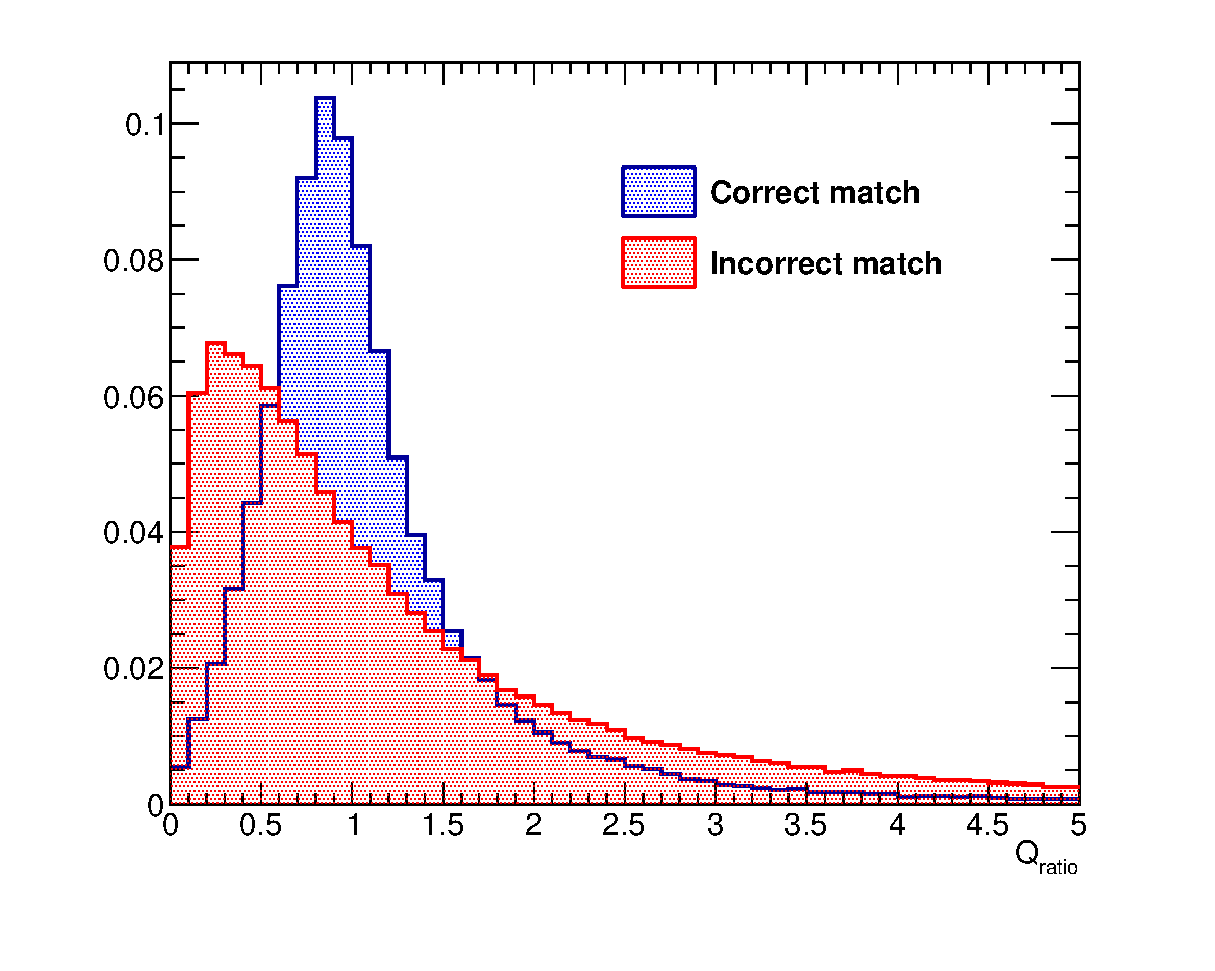
\includegraphics[width=7cm]{images/hough_3d_matching/3DMatching_Barrel_2Track_QRatio_Separation.eps} \label{fig:3DMatchingBarrel2TrackQRatioSeparation}}
  \subfloat[$Q_{\textrm{ratio}}$ probability density distribution.]{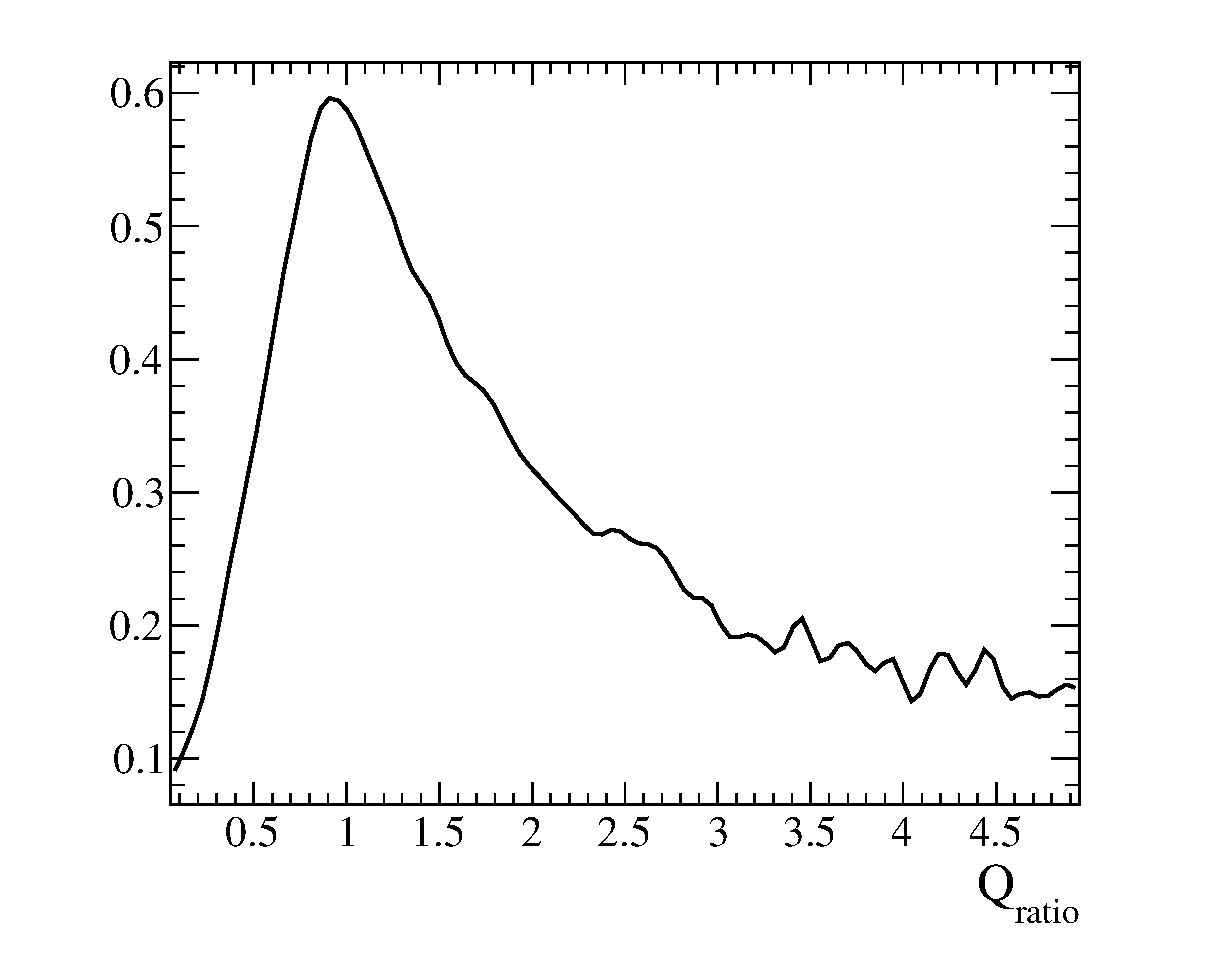
\includegraphics[width=7cm]{images/hough_3d_matching/3DMatching_Barrel_2Track_QRatio_PDF.eps} \label{fig:3DMatchingBarrel2TrackQRatioPDF}}
  \caption{$Q_{\textrm{ratio}}$ and its probability density distribution in the barrel ECal for the two track case.}
  \label{fig:QRatio}
\end{figure}
%\begin{figure}
%  \centering
%  \parbox{7cm}{
%    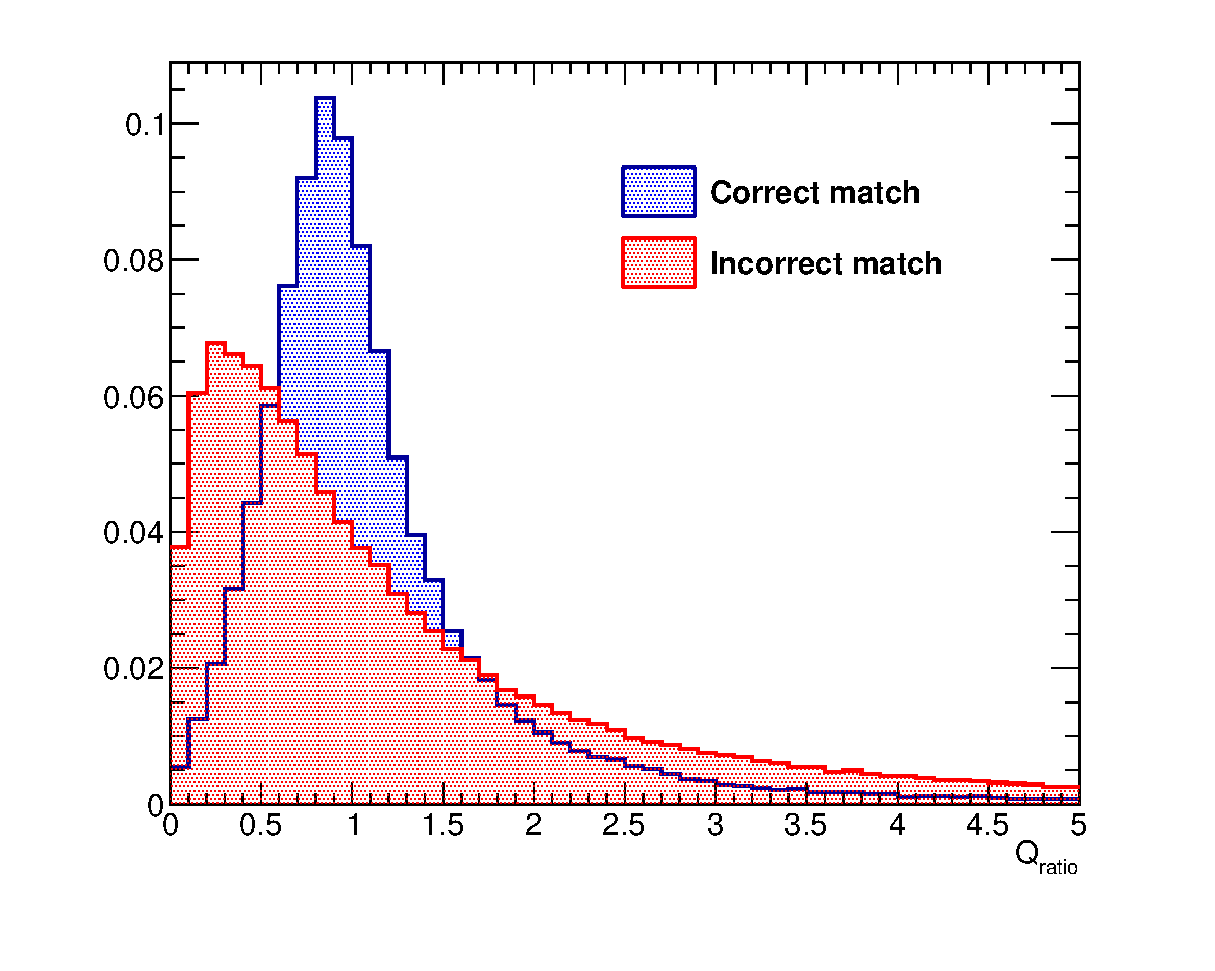
\includegraphics[width=7cm]{images/hough_3d_matching/3DMatching_Barrel_2Track_QRatio_Separation.eps}
%    \caption{$Q_{\textrm{ratio}}$ distribution in the barrel ECal for the two track case.  The blue distribution refers to matching pairs which were matched to the same true particle.  Both distributions are unit normalised.}
%    \label{fig:3DMatchingBarrel2TrackQRatioSeparation}}
%    \qquad
%    \begin{minipage}{7cm}
%      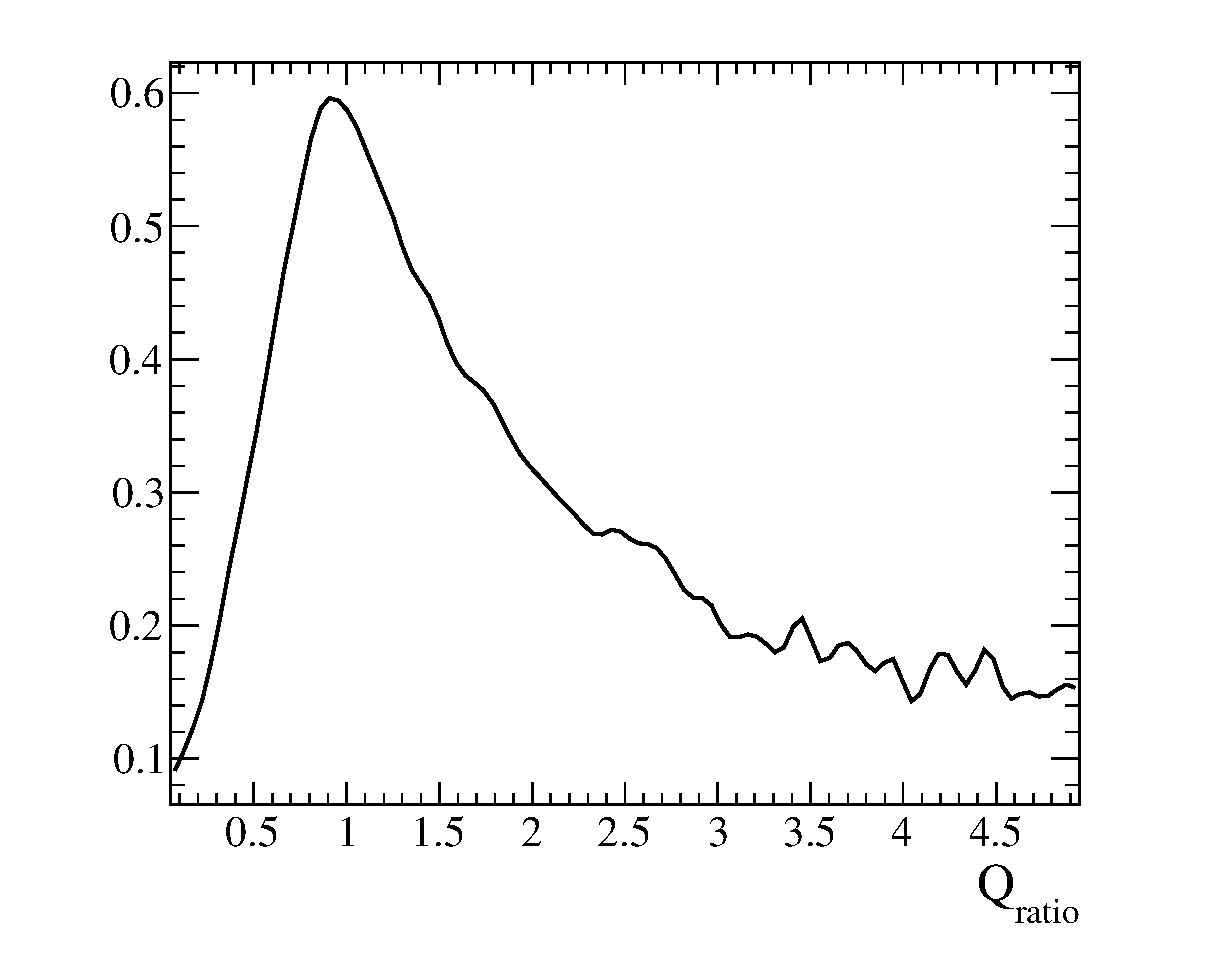
\includegraphics[width=7cm]{images/hough_3d_matching/3DMatching_Barrel_2Track_QRatio_PDF.eps}
%      \caption{$Q_{\textrm{ratio}}$ probability density distribution in the barrel ECal for the two track case.}
%      \label{fig:3DMatchingBarrel2TrackQRatioPDF}
%    \end{minipage}
%\end{figure}
\newline
\newline
The second input to the likelihood, called $\Delta_{\textrm{layer, first}}$, is the difference in the starting layer of each 2D track which forms the matching candidate pair, where starting layer refers to the layer closest to the ND280 tracker.  For 2D tracks which should be matched together, $\Delta_{\textrm{layer, first}}$ should be 1.  The separation ability of this variable for the two track, barrel is shown in Fig.~\ref{fig:3DMatchingBarrel2TrackDFLSeparation}.  The discreet probability density function was created using eqn.~\ref{eq:BinProbabilityPDF}.  It was not necessary to interpolate using splines as $\Delta_{\textrm{layer, first}}$ is itself discreet.  The probability density function for $\Delta_{\textrm{layer, first}}$ is shown in Fig.~\ref{fig:3DMatchingBarrel2TrackDFLPDF} for the two track, barrel case.  For each matching candidate pair, the value of $\Delta_{\textrm{layer, first}}$ is calculated and the corresponding $\mathcal{L}_{\Delta_{\textrm{layer, first}}}$ is retrieved from the probability density function.
\begin{figure}%
  \centering
  \subfloat[$\Delta_{\textrm{layer, first}}$ distribution (area normalised).  The blue and red distributions refers to matching pairs which were matched to the same true particle and different true particles respectively.]{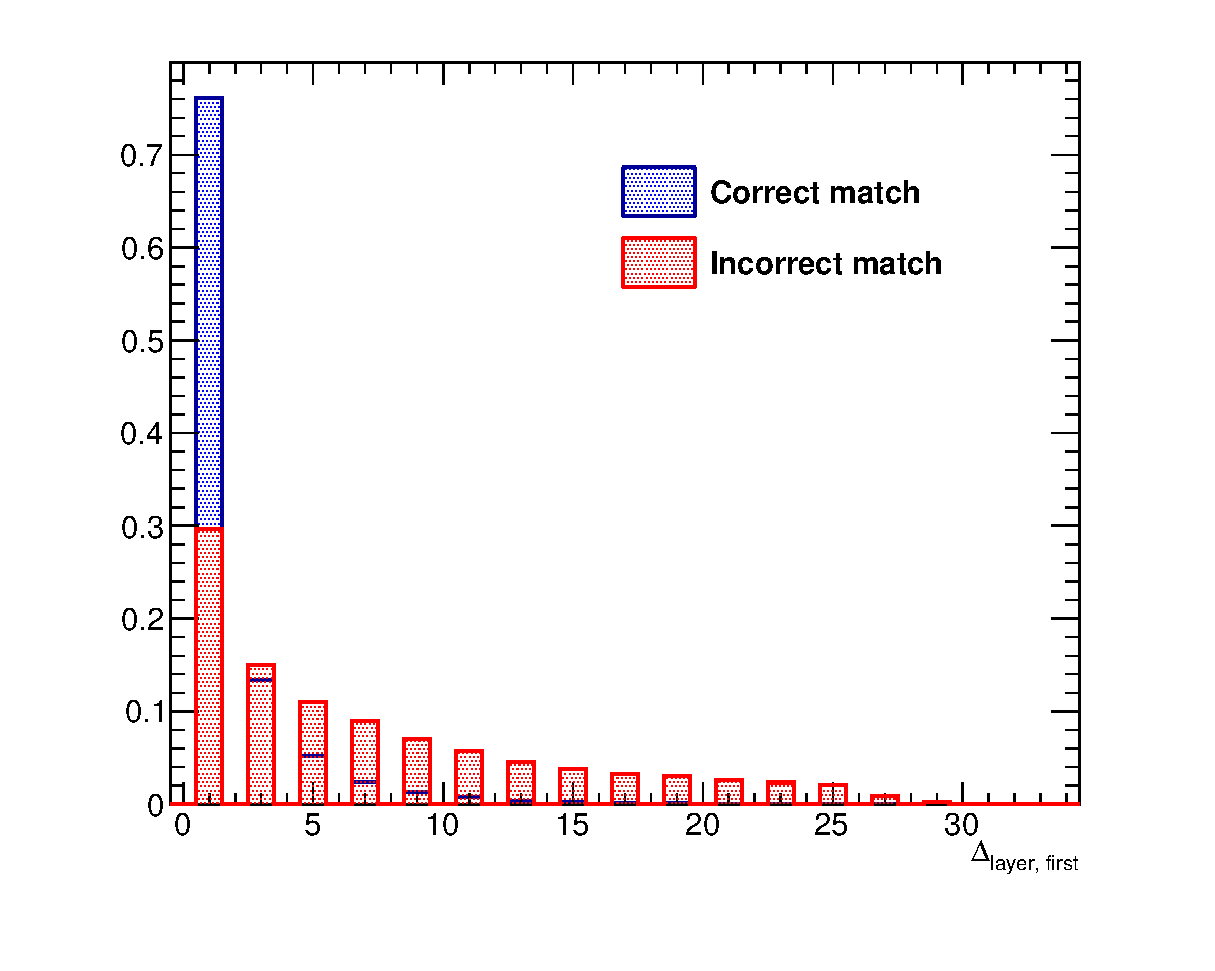
\includegraphics[width=7cm]{images/hough_3d_matching/3DMatching_Barrel_2Track_DFL_Separation.eps} \label{fig:3DMatchingBarrel2TrackDFLSeparation}}
  \subfloat[$\Delta_{\textrm{layer, first}}$ probability density distribution.]{\includegraphics[width=7cm]{images/hough_3d_matching/3DMatching_Barrel_2Track_DFL_PDF.eps} \label{fig:3DMatchingBarrel2TrackDFLPDF}}
  \caption{$\Delta_{\textrm{layer, first}}$ and its probability density distribution in the barrel ECal for the two track case.}
  \label{fig:DFL}
\end{figure}
%\begin{figure}
%  \centering
%  \parbox{7cm}{
%    \includegraphics[width=7cm]{images/hough_3d_matching/3DMatching_Barrel_2Track_DFL_Separation.eps}
%    \caption{$\Delta_{\textrm{layer, first}}$ distribution in the barrel ECal for the two track case.  The blue distribution refers to matching pairs which were matched to the same true particle.  Both distributions are unit normalised.}
%    \label{fig:3DMatchingBarrel2TrackDFLSeparation}}
%    \qquad
%    \begin{minipage}{7cm}
%      \includegraphics[width=7cm]{images/hough_3d_matching/3DMatching_Barrel_2Track_DFL_PDF.eps}
%      \caption{$\Delta_{\textrm{layer,first}}$ probability density distribution in the barrel ECal for the two track case.}
%      \label{fig:3DMatchingBarrel2TrackDFLPDF}
%    \end{minipage}
%\end{figure}
\newline
\newline
The third and final input to the likelihood, called $\Delta_{\textrm{layer, last}}$, is the differnce in the ending layer of each 2D track which forms the matching cadidate pair, where the ending layer refers to the layer furthest from the ND280 tracker.  Functionally, how this function is used is essentially identical to $\Delta_{\textrm{layer, last}}$ so it will not be described in detail.  The separation ability of this variable and its corresponding probabilty density function for the two track, barrel case are shwon in Fig.~\ref{fig:3DMatchingBarrel2TrackDLLSeparation} and Fig.~\ref{fig:3DMatchingBarrel2TrackDLLPDF} respectively.
\begin{figure}%
  \centering
  \subfloat[$\Delta_{\textrm{layer, last}}$ distribution (area normalised).  The blue and red distributions refers to matching pairs which were matched to the same true particle and different true particles respectively.]{\includegraphics[width=7cm]{images/hough_3d_matching/3DMatching_Barrel_2Track_DLL_Separation.eps} \label{fig:3DMatchingBarrel2TrackDLLSeparation}}
  \subfloat[$\Delta_{\textrm{layer, last}}$ probability density distribution.]{\includegraphics[width=7cm]{images/hough_3d_matching/3DMatching_Barrel_2Track_DLL_PDF.eps} \label{fig:3DMatchingBarrel2TrackDLLPDF}}
  \caption{$\Delta_{\textrm{layer, last}}$ and its probability density distribution in the barrel ECal for the two track case.}
  \label{fig:DLL}
\end{figure}
%\begin{figure}
%  \centering
%  \parbox{7cm}{
%    \includegraphics[width=7cm]{images/hough_3d_matching/3DMatching_Barrel_2Track_DLL_Separation.eps}
%    \caption{$\Delta_{\textrm{layer, last}}$ distribution in the barrel ECal for the two track case.  The blue distribution refers to matching pairs which were matched to the same true particle.  Both distributions are unit normalised.}
%    \label{fig:3DMatchingBarrel2TrackDLLSeparation}}
%    \qquad
%    \begin{minipage}{7cm}
%      \includegraphics[width=7cm]{images/hough_3d_matching/3DMatching_Barrel_2Track_DLL_PDF.eps}
%      \caption{$\Delta_{\textrm{layer,last}}$ probability density distribution in the barrel ECal for the two track case.}
%      \label{fig:3DMatchingBarrel2TrackDLLPDF}
%    \end{minipage}
%\end{figure}
\newline
\newline
The matching likelihood, $\mathcal{L}$, for a matching candidate pair is then
\begin{equation}
  \mathcal{L} = \mathcal{L}_{Q_{\textrm{ratio}}} \times \mathcal{L}_{\Delta_{\textrm{layer, first}}} \times \mathcal{L}_{\Delta_{\textrm{layer, last}}}.
\end{equation}
As described above, $\mathcal{L}$ is calculated for every matching candidate pair and the pair which maximise $\mathcal{L}$ is selected as a match and removed from the pool.  The process is then repeated until no more matches can be made.
\newline
\newline
3D tracks have now been formed, but the associated directions and positions of those tracks still need to be calculated.  The track fitting process for the newly formed 3D tracks is very similar to that described in section~\ref{subsec:ECal3DHitReconstruction}.  The tracks are briefly separated into their constituent 2D views and a charge-weighted average position of each layer is calculated using the track's constituent hits.  Then, the hits in the opposing view are used to estimate the 3rd coordinate of a given layer using a least-squares fit.  After all of the coordinates have been estimated, a full 3D least-squares fit of the positions in each layer is performed to estimate the 3D track's direction and position in that ECal layer.

\subsection{Track splitting}
\label{subsec:TrackSplitting}
During development of the reconstruction, it became clear that a certain topology had been overlooked.  An example of this is shown in Fig.~\ref{fig:MergedTrackEventDisplay} which shows a MC neutrino interaction in the ECal with 3 charged final states.  As can be seen from Fig.~\ref{fig:MergedTrackEventDisplay}, the muon (solid green line) is emitted back-to-back with one of the final-state protons (solid blue line) in this ECal view.  Because the Hough transform implementation only concerns itself with straight lines, the result is that such back-to-back trajectories are typically reconstructed as a single track.  However, there are two views available for every ECal module and the back-to-back emittence typically only appears in the ECal view which is perpendicular to the beam direction (the XY view).  So, the correctly reconstructed tracks in the other ECal view can be used to split the tracks in the problematic view.  
\begin{figure}
  \centering
  \includegraphics[width=7cm]{images/hough_3d_matching/MergedTrackEventDisplay.pdf}
  \caption{Event display of a problematic (for the reconstruction) neutrino interaction in the ECal.  The solid green track is the muon, the solid blue tracks are protons and the pink tracks are neutrons.  The neutrino is the short dashed green line.}
  \label{fig:MergedTrackEventDisplay}
\end{figure}
\newline
\newline
Consider a neutrino interaction with two charged final-states which has been reconstructed as one track in one view (called the merged view) but reconstructed as two tracks in the other view (called the other view).  It should be expected that the single track in the merged view is not a particularly good match for either of the tracks in the other view.  However, if the two tracks in the other view were temporarily merged together and this new track was compared to the single track in the merged view, one should expect this match to return a much higher value of $\mathcal{L}$.  This feature can be used to identify a potentially merged track in a given view.
\newline
\newline
This motivated an extension to the 3D matching aspect of the reconstruction.  As a reminder, the 3D matching algorithm makes every pairwise comparison of tracks from each view to find the pair which maximise $\mathcal{L}$.  This matching routine was modified to also include temporary mergings of every pairwise combination of tracks in a single view.  These temporary mergings can then be compared to every single track in the other view.  As an example, consider a situation where 3 tracks (labelled $A$, $B$ and $C$) have been reconstructed in one view and two tracks (labelled $Y$ and $Z$) have been reconstructed in the other view.  With the old method, the following comparisons would be made:
\begin{equation}
\begin{split}
A &\longleftrightarrow Y \\
A &\longleftrightarrow Z \\
B &\longleftrightarrow Y \\
B &\longleftrightarrow Z \\
C &\longleftrightarrow Y \\
C &\longleftrightarrow Z
\end{split}
\label{eq:TrackSplittingOldMethod}
\end{equation}
With the new method, which includes temporarily merged pairs of tracks in a given view, the following comparisons would be made:
\begin{equation}
\begin{split}
A &\longleftrightarrow Y \\
A &\longleftrightarrow Z \\
B &\longleftrightarrow Y \\
B &\longleftrightarrow Z \\
C &\longleftrightarrow Y \\
C &\longleftrightarrow Z \\
A+B &\longleftrightarrow Y \\
A+B &\longleftrightarrow Z \\
A+C &\longleftrightarrow Y \\
A+C &\longleftrightarrow Z \\
B+C &\longleftrightarrow Y \\
B+C &\longleftrightarrow Z \\
A &\longleftrightarrow Y+Z \\
B &\longleftrightarrow Y+Z \\
C &\longleftrightarrow Y+Z
\end{split}
\label{eq:TrackSplittingNewMethod}
\end{equation}
In terms of the matching comparisons, the temporarily merged comparisons are treated on the same footing as the single track comparisons; $\mathcal{L}$ is calculated for each comparison and the one which maximises $\mathcal{L}$ is selected.  However, the post-matching treatment of the best match depends on whether a temporary merge is involved.  If the match which maximises $\mathcal{L}$ involves two single tracks then the treatment is as before; they are removed from the pool and the process is repeated.  If a temporarily merged pair are involved, the 2D crossing location of the temporarily merged tracks is calculated and is then used to split the single track in the other view.  The original track is removed from the pool and replaced by the two single tracks formed from the split.  The matching process is then begun again and repeated until all matches have been made.

\subsection{Track pairwise crossing reconstruction}
\label{subsec:TrackCrossingReconstruction}
The final step of the reconstruction is to estimate where each of the 3D track's paths cross.  As each track is reconstructed as a straight line in 3D, the final step is fairly simple.  Using the track direction and position information calculated at the end of section~\ref{subsec:3DHoughTrackReconstruction}, the position at closest approach for every pairwise combination of 3D tracks is calulated analytically.  The distance of closest approach is also calculated.  Six hits, the closest three from each 3D track, are then associated to the pairwise crossing. 

\section{Output of the reconstruction}
\label{sec:ReconOutput}
The reconstruction is run over every 3D cluster found in the ECal.  By applying the steps outlined above, for each 3D cluster the following output is given:
\begin{itemize}
  \item A set of 3D tracks
  \item The pairwise crossings of all 3D tracks found in the cluster
\end{itemize}
Note that no vertex formation beyond the pairwise crossings is calculated at this stage, nor is any analysis of the 3D tracks performed.  While this may seem like an oversight of the reconstruction, this approach was decided as no assumptions are made about what the tracks/crossings represent at this point, making the output more generic.  Any analysis which wants to make use of the reconstruction is given enough information to apply more targeted reconstruction downstream. 


%
%To build the probability density distributions, the output of the 2D reconstruction was used to form every possible matching pair (as described above) and the results were separated into two distinct categories: correctly matched and incorrectly matched.
\section{Validation of the reconstruction}
\label{sec:ReconstructionValidation}
Because of the large scope of the reconstruction and the limited time available for the presented analysis, the validation of the reconstruction was done in parallel to the rest of the analysis and is still an ongoing effort.  The validation that has been done can be split into two areas: validation of the performance of the algorithms purely using MC and comparisons of MC to data using control samples.
\newline
\newline
The first performance validation investigated the angular resolution using the enhanced reconstruction (by L. Pickering).  This study calculated the angular resolution for MC muons fired into the side-left ECal for a range of entry angles.  For each MC event, the cosine of the angular separation between the true particle angle and the reconstructed angle was calculated, $\cos\theta^{\textrm{Sep}}$.  The values of $\cos\theta^{\textrm{Sep}}$ were then binned in a distribution.  An outward scan from the peak of the distribution was then performed to find where the height decreased to $68\%$ of the peak.  The value of $\theta^{\textrm{Sep}}$ and this point was taken as the angular resolution.  These results are shown in Fig.~\ref{fig:MuonAngularResolutionDSECal}.  Generally speaking, the found angular resolutions are very good.  For long trajectories (200~mm), the angular resolution is within 15$^\circ$.  It is only for short tracks (40~mm) that the angular resolution becomes large.
\begin{figure}
  \centering
  \includegraphics[width=9cm]{images/hough_validation/MuonAngularResolutionDSECal}
  \caption{The angular resolution as a function of trajectory length in the DS-ECal when applying the enhanced reconstruction to muon MC.  The colour coding refers to the true entry angle range of the muons.}
  \label{fig:MuonAngularResolutionDSECal}
\end{figure}
\newline
\newline
The second performance validation studied the success of the 3D matching.  To do this, a sample of beam MC events in the ECals were processed through the enhanced reconstruction.  After completion, the 2D components of the 3D tracks were analysed and matched to the true particles which created them.  A match was counted as a success if both 2D components were matched to the same true particle.  These results are shown in table~\ref{table:PercentageCorrect3DMatching}, separated out by which track matching likelihood was used.  For the 1 and 2 track likelihood cases, the matching performs very well.  It is only in cases where the 3 track likelihood is used that the matching start to suffer slightly.  However, all of the correct matching rates are well above 50$\%$ which suggests that the 3D matching is performing adequetly. 
\begin{table}
  \begin{tabular}{c | c c c }
   & 1 track likelihood & 2 track likelihood & 3 track likelihood \\ \hline \hline
   $1^{\textrm{st}}$ track matched& 96$\%$ & 92$\%$ & 80$\%$ \\
   $2^{\textrm{nd}}$ track matched&  & 89$\%$ & 79$\%$ \\
   $3^{\textrm{rd}}$ track matched&  &  & 70$\%$ \\
  \end{tabular}
  \caption{The percentage number of correct matches in the 3D matching separated by which track matching likelihood was used.}
  \label{table:PercentageCorrect3DMatching}
\end{table}


  %\chapter{Magnetic field simulation in ND280}
\label{chap:MagneticFieldSimulation}
ND280 is housed in the \Yoshi{former}{it isn't the UA1 magnet any more!} UA1 magnet which provides a \Yoshi{0.18}{It's not a 0.2 T field any more!}~T magnetic field through the basket.  The purpose of this magnetic field is to aid particle \Yoshi{identification}{was identifcation} \Yoshi{and momentum measurements}{not just PID} in ND280's TPCs.  This magnetic field is accurately modelled in nd80mc by a constant 0.18 T magnetic field in the basket.  The ND280 analyses, which are inputs to the oscillation analyses, search for a TPC track matched to an FGD track so, in a first iteration of these analyses, the magnetic field model is sufficient for its purpose.
\newline
\newline
However, a significant part of the UA1 magnet is the iron based, magnetic flux return yoke which helps to tightly contain the magnetic field outside of the tracker region.  As a result, there is a significant magnetic field contained within the magnetic flux return yoke during operation.  This magnetic field in the flux return yoke is not modelled in nd280mc.  For the first iterations of the ND280 oscillation input analyses, this approximation was valid.  However, as the ND280 analyses become more mature, and non-tracker based analyses are started, this approximation is no longer sufficient.  So, the magnetic field model in the simulation needs revising.
\newline
\newline
\Yoshi{The Monte Carlo event rates seen in the ECals are directly affected by mismodelling of the magnetic field in the yokes which can have very serious consequences for any ECal-based analysis.  So, the following chapter presents the first investigation of the magnetic field's effect in this region and an improvement to the magnetic field model.  This model improvement has now been incorporated into the official ND280 MC simulations which is used by all physics analyses at ND280.}{I would add something like ``As one of the analysers who has been central to studying events occurring in the ECals, which are directly affected by mismodelling of the magnetic field in the yokes, I was the first T2K collaborator to investigate this effect and provide an improved field model; this was subsequently adopted as the field to be used in official ND280 MC simulations, used by all physics analyses at ND280.}

\section{Magnetic field model in the ND280 flux return}
\label{sec:MagneticFieldModel}
\begin{figure}
  \centering
  \includegraphics[width=9cm]{images/magnetic_field/ND280FluxReturn}
  \caption{Graphical display of the X-Y ND280 cross-section.}
  \label{fig:ND280FluxReturn}
\end{figure}
A simple model for the magnetic field in the flux return can be found by making two assumptions.  Firstly, the flux return yoke consists mostly of iron which has a much higher magnetic permeability than the air surrounding it.  So, it can be assumed that any magnetic flux passing through the ND280 basket is solely transported back around by the return yoke (no flux passes through the atmosphere in the pit).  It follows that
\begin{equation}
  \phi_{\textrm{b}} = \phi_{\textrm{r}},
  \label{eqn:BFluxConservation}
\end{equation}
where $\phi_{\textrm{b}}$ is the magnetic flux passing through the tracker and $\phi_{\textrm{r}}$ is the magnetic flux passing through the return yoke.  The second assumption regards the shape of the ND280 basket and flux return yoke.  The X-Y cross-section of ND280, as shown in Fig.~\ref{fig:ND280FluxReturn}, can be modelled as two distinct parts: the flux return yoke and everything contained within.  It is clear from Fig.~\ref{fig:ND280FluxReturn} that both areas are \Yoshi{rectangular}{retangular} so the system can be modelled as a smaller rectangle (the basket) contained within a larger rectangle (the return yoke).  Using this assumption and Eq.~\ref{eqn:BFluxConservation}, the magnetic field strength passing through the return yoke, $B_{r}$, is
\begin{equation}
  B_{\textrm{r}} = \frac{B_{\textrm{b}}A_{\textrm{b}}}{A_{\textrm{r}} - A_{\textrm{b}}},
  \label{eqn:FluxReturnBField}
\end{equation}
where $B_{\textrm{b}}$ is the strength of the magnetic field passing through the basket, $A_{\textrm{b}}$ is the cross-sectional area of the basket region and $A_{\textrm{r}}$ is the cross-sectional area of the flux return yoke if the flux return yoke was not hollow.
\newline
\newline
\begin{figure}
  \centering
  \includegraphics[width=9cm]{images/magnetic_field/BFieldDiagram}
  \caption{Simple model of the magnetic field in the basket and flux return region.  The flux return yoke has been separated into ten sections: four vertical B field sections, four corner B field sections and two horizontal B field sections.  The height of the basket region, $h$, is also shown.}
  \label{fig:BFieldDiagram}
\end{figure}
Eq.~\ref{eqn:FluxReturnBField} is sufficient to model the strength of the magnetic field in the flux return yoke, yet Eq.~\ref{eqn:FluxReturnBField} conveys no information about the direction of the magnetic field.  However, the direction can be estimated by separating the flux return into ten sections as shown in Fig.~\ref{fig:BFieldDiagram}.  The sections are: four vertical sections where the magnetic field enters and exits the flux return region, two horizontal sections where the magnetic field in the flux return is anti-parallel to the magnetic field in the basket and four corner sections where the magnetic field transitions between the horizontal and vertical sections.  By defining the magnetic field in the basket to be parallel to the $x$-axis 
\begin{equation}
  \overrightarrow{B_{\textrm{b}}} = {B_{\textrm{b}}}\hat{\imath},
  \label{eqn:BasketBFieldVector}
\end{equation}
\Yoshi{where $\imath$ is the unit vector in the $x$ direction}{need to define stuff properly.}
then it follows that the horizontal magnetic field in the flux return is
\begin{equation}
  \overrightarrow{B}^{\textrm{H}}_{\textrm{r}} = -{B_{\textrm{r}}}\hat{\imath}.
  \label{eqn:HorizontalReturnBFieldVector}
\end{equation}
The field model for the vertical section should take into account that the strength of the magnetic field is not constant, but increases in strength until it reaches the corner region\Yoshi{}{What is the corner section? And reaching it from which direction?}.  The direction of the field depends on which vertical section is under consideration.  For the section where\Yoshi{}{can this be explained graphically? It's hard to follow what you mean. It's not absolutely needed, but it would make it easier for the reader...} the magnetic field is exiting the tracker and moving upwards, the relevant vector is
\begin{equation}
  \overrightarrow{B}^{\textrm{V}}_{\textrm{r}} = \frac{y}{h/2}{B_{\textrm{r}}}\hat{\jmath},
  \label{eqn:VerticalReturnBFieldVector}
\end{equation}
where $h$ is the height of the ND280 basket and $y$ is the height at which the magnetic field is being evaluated in the ND280 coordinate system.  In the corner regions, the magnetic field is defined to be straight, constant in strength and at 45$^\circ$ to the horizontal and vertical sections.  As with the vertical section, the magnetic field direction is dependent on which corner section is being considered.  For the corner section where the magnetic field is exiting the tracker and travelling vertically upwards (as defined in Eq.~\ref{eqn:VerticalReturnBFieldVector}), the vector is
\begin{equation}
  \overrightarrow{B}^{\textrm{C}}_{\textrm{r}} = \frac{B_{\textrm{r}}}{\sqrt{2}}(\hat{\jmath} - \hat{\imath}).
  \label{eqn:CornerReturnBFieldVector}
\end{equation}
The magnetic field in the other corner sections are then 45$^\circ$ rotations of Eq.~\ref{eqn:CornerReturnBFieldVector}.
\newline
\newline

\section{Effect of magnetic field on the ECal}
\label{sec:MagneticFieldEffect}
%This simple model of the magnetic field in the flux return has now been implemented in nd280mc.  Thus, any simulated charged-particles trajectory in the region surrounding the ECals (like muons entering from the pit region) will be altered by the new field.
\begin{figure}%
  \centering
  \subfloat[Number of hits in the reconstructed cluster.]{\includegraphics[width=9cm]{images/magnetic_field/NHits_BLB_NoField} \label{fig:NHitsBLBNoField}}
  \subfloat[The truncated max ratio of the reconstructed cluster.]{\includegraphics[width=8cm]{images/magnetic_field/TMR_BLB_NoField}\label{fig:TMRBLBNoField}}

  \caption{Comparisons of data and Monte Carlo in the bottom-left barrel ECal for previous software productions.  The red and pink histograms are Monte Carlo simulation of T2K beam neutrinos incident on ND280 and the surrounding pit respectively.  The blue data points are collected data from run 3C.  Both of the plots are POT normalized.}
  \label{fig:BLBNoField}
\end{figure}
It was found in previous iterations of ND280 analyses that there were significant discrepancies between the Monte Carlo and the collected data in the ECal.  The discrepancies found had an ECal module dependence where the bottom modules were affected most.  The problem appeared in the low-level distributions, such as how many scintillator hits were assigned to each reconstructed object.  An example of this is shown in Fig.~\ref{fig:NHitsBLBNoField} which shows a comparison of Monte Carlo with run 3C data for the number of constituent hits in each reconstructed object measured in the bottom-left barrel ECal.  For the number of hits region with high population (between roughly 10 and 30) there is a clear excess of collected data events.  As the high level variables, such as the ones used for track-shower discrimination, are based on these low-level quantities, the discrepancy propagated through causing significant disagreement at all levels.  An example of this effect is shown in Fig.~\ref{fig:TMRBLBNoField} which shows a data and Monte Carlo comparison, again for the bottom-left barrel ECal, for the Truncated Max Ratio (TMR) of the reconstructed objects.  The TMR, which calculates the ratio of the lowest total charge found in an ECal layer to the high total charge in an ECal layer after removing the top and bottom 20$\%$ of hits, is an input into the track-shower discriminator described in section~\ref{subsec:ECalParticleIdentification}.  The track-shower discrimination is a key feature of the ECal reconstruction which is used by several ND280 analyses so such a big discrepancy is a serious problem.
\newline
\newline
As ND280 is off-axis relative to the T2K beam, there is an increase in the neutrino flux in the flux return yoke and surrounding pit regions below the bottom ECals.  This means that any charged final states in this region would generally have to propagate through the flux return yoke.  If a magnetic field is present in this region, as there would be during data taking, the trajectory of such particles would be bent upwards towards the ND280 tracker region, causing an increase in the event rate in the bottom ECals.  If the magnetic field in this region is missing, the above statement does not hold and a relative deficit of events would be seen which describes the situation seen in Fig.~\ref{fig:BLBNoField}.
\begin{figure}[bottom]%
  \centering
  \subfloat[Number of hits in the reconstructed cluster.]{\includegraphics[width=8cm]{images/magnetic_field/NHits_BLB_WithField} \label{fig:NHitsBLBWithField}}
  \subfloat[The truncated max ratio of the reconstructed cluster.]{\includegraphics[width=8cm]{images/magnetic_field/TMR_BLB_WithField}\label{fig:TMRBLBWithField}}
  \caption{Comparisons of data and Monte Carlo in the bottom-left barrel ECal with the magnetic field model described in section~\ref{sec:MagneticFieldModel} implemented.  The red and pink histograms are Monte Carlo simulation of T2K beam neutrinos incident on ND280 and the surrounding pit respectively.  The blue data points are collected data from run 3C.  Both of the plots are POT normalized.}
  \label{fig:BLBWithField}
\end{figure}
So, the simple magnetic field model in the flux return yoke described in section~\ref{sec:MagneticFieldModel} was implemented in nd280mc and a batch of beam and \Yoshi{sand Monte Carlo}{``sand Monte Carlo'' is very much jargon. Introduce it properly} was produced to test its effect.  To get an idea of the magnetic field's effect on the rates measured by the ECals, the same variables as shown in Fig.~\ref{fig:BLBNoField} are shown in Fig.~\ref{fig:BLBWithField}, but with the magnetic field activated.  The difference is very clear; Fig.~\ref{fig:NHitsBLBWithField} shows that the excess in the 10 to 30 hits region is now gone.  It is also clear that the effect of the magnetic field has propagated through to the high level discriminators, as shown in Fig.~\ref{fig:TMRBLBWithField}.
\newline
\newline
Despite this study only briefly investigating the presence of a magnetic field in the UA1 flux return yoke, the improvement provided is undeniable.  It was decided that the model would be a permanent feature of the ND280 simulation and is now used in all software productions including the inputs to this analysis.

  %\chapter{Selection of neutrino interactions in the ECal}
\label{chap:NeutrinoInteractionSelection}
This analysis presents a measurement of the CC inclusive interaction cross-section of $\nu_\mu$ with lead nuclei using the ND280 \Yoshi{Tracker}{ADDRESSED - I would say that ``Tracker'' is a proper noun, the name of the detector, so it should be capitalised throughout. The detector name is then ``Tracker ECal''} ECals.  To make such a measurement, a sample of neutrino interaction vertices within the ECal must be found.  The selection of events is based on the enhanced reconstruction outlined in chapter~\ref{chap:EnhancedECalReconstruction}, which was specifically designed to \Yoshi{be sensitive to}{ADDRESSED - introduce} track multiplicity.  As a result of this method, vertices in the ECal are naturally separated into topologies defined by the number of reconstructed tracks.  Any selection development should take advantage of this situation and tailor cuts to be specific to each topology, which should result in a higher overall sample purity.  The 3D track matching aspect of the reconstruction was only tuned to handle up to three tracks simultaneously.  However, this analysis aims to measure a CC-inclusive cross-section so it should not be biased against any neutrino energy range.  \Yoshi{There is a deep connection between the number of reconstructed tracks and the energy of the neutrino that created them.  The number of reconstructed tracks should correlate with the number of final state particles involved with the neutrino interaction and the number of final state particles correlates with the energy of the interacting neutrinos.  Therefore it is important to not reject events based solely on the number of reconstructed tracks}{ADDRESSED - state the implied connection between number of prongs and neutrino energy}.  Bearing this information in mind, the selection should separate out the events into the following topologies:
\begin{itemize}
  \item 1 prong topology
  \item 2 prong topology
  \item 3 prong topology
  \item 4+ prong topology
\end{itemize}
The definition of a prong is a reconstructed track associated with a reconstructed vertex.
\newline
\newline
However, as described in section~\ref{sec:ReconOutput}, the output of the enhanced reconstruction has been kept generic and is not specifically tailored to this task.  The reconstruction outputs a set of clusters which contain a set of 3D tracks and every pairwise crossing that said tracks make.  While it is true that in some situations the reconstruction will accurately represent a vertex ``out of the box''---e.g., when only two tracks are reconstructed in the cluster---there will be many situations where extra reconstruction steps are needed before any further selection can take place.  \Yoshi{Hence}{ADDRESSED - I wouldn't start a sentence with ``So,''---it seems like spoken English to me. I'd say ``Hence'' with no comma} the structure of this chapter is as follows: the definition of signal is described first along with the sample used to develop the selection, followed by a discussion of the vertex reconstruction.  After the final reconstruction steps have been discussed, a full discussion of the neutrino selection follows.

\section{Signal definition}
\label{sec:SignalDefinition}
The measurement \Yoshi{that is the intended outcome}{ADDRESSED - ``measurement of this analysis''} of this analysis is the CC inclusive interaction cross-section of $\nu_\mu$ with lead nuclei using the ND280 Tracker ECals.  The active volume of the ECal consists of layers of plastic scintillator and lead absorbers.  Neutrino interactions that occur in the lead absorbers are indistinguishable from those that occur in the plastic scintillator.  Because of this fact, the selection does not attempt to separate the two cases out.  So, the strict signal definition used by this selection  is as follows:
\begin{itemize}
  \item Interacting neutrino is flavour $\nu_\mu$
  \item Interaction type is charged current
  \item Interaction occurs within the active volumes of either the barrel ECal or DS ECal
\end{itemize}
The active volume is defined by the ROOT geometry used in the simulation.  Specifically, it is a rectangular box which encompasses all of the lead and scintillator layers for each ECal module.  Any target element contained within this volume is a signal target.

\section{Monte Carlo sample}
\label{sec:MonteCarloSample}
NEUT was used to generate a neutrino beam sample of Monte Carlo events which corresponds to $3.949\times10^{20}$ POT.  All of this sample was generated using a simulated beam power of 178 kW which is the average beam power used for Run III.  At this intensity, there are an expected 9.46 neutrino interactions per eight bunch spill in ND280.  So, there will be approximately one interaction per bunch across the entire \Yoshi{}{ADDRESSED - was `of'} ND280, meaning the chance of pileup is small. 
\newline
\newline
The sample \Yoshi{described}{ADDRESSED} above only simulated neutrino interactions within ND280 (including the \Yoshi{outermost}{ADDRESSED - was `surrounding'} magnet).  However, we expect many interactions in the surrounding pit (referred to as ``sand interactions'' from now on) to have final states which enter ND280.  So, NEUT was used to generate an additional sample of sand interactions (hereafter referred to as sand Monte Carlo) which corresponds to $3.708\times10^{20}$\Yoshi{~POT}{ADDRESSED}.  There is roughly a 6$\%$ difference in the POT of the beam and sand Monte Carlo.  As the sand Monte Carlo has a sufficiently high level of statistics, scaling the smaller sample to match the larger is acceptable.
\newline
\newline
\begin{table}
  \begin{tabular}{ l r }
    ECal module & No. signal events \\ \hline \hline
    Bottom-right & 223042 \\
    Side-right & 231955 \\
    Top-right & 135476 \\
    Bottom-left & 262500 \\
    Side-left & 293065 \\
    Top-left & 140539 \\
    Downstream & 134100 \\
    \hline
    Total & 1420677 \\
  \end{tabular}
  \caption{The number of signal events in the NEUT-based beam Monte Carlo sample separated by ECal module.}
  \label{table:NSignalEventsTruth}
\end{table}
The number of signal interactions from the Monte Carlo sample is shown in table~\ref{table:NSignalEventsTruth}, separated into the ECal module they occurred in.  The number of signal interactions is also shown as a function of neutrino energy for the bottom-left, top-right and DS ECals in Fig.~\ref{fig:NSignalEventsTruthNeutrinoEnergy}.  Clearly, there are an extremely high number of signal events in the sample, which means that the statistical error in this analysis should be small.  As an example, consider a selection with a 1$\%$ signal efficiency in the DS ECal.  Assuming $100\%$ selected sample purity, the number of selected events would be 1341 which corresponds to a statistical error of 2.73$\%$.  Even in this extremely unrealistic situation, the statistical error is small.
\begin{figure}
  \centering
  \includegraphics[width=12cm]{images/selection/signal_definition/NSignalEventsNeutrinoEnergy.eps}
  \caption{The number of signal events in the NEUT-based beam Monte Carlo sample as a function of neutrino energy in the bottom-left (red), top-right (blue) and DS (black) ECals.  The bottom-left ECal sees the most signal events and at a higher neutrino energy which is caused by the off-axis effect.}
  \label{fig:NSignalEventsTruthNeutrinoEnergy}
\end{figure}
\section{Vertex reconstruction}
\label{sec:VertexReconstruction}
\Yoshi{The following section outlines the algorithm developed to reconstruct vertices in the ECal using the enhanced reconstruction described in chapter~\ref{chap:EnhancedECalReconstruction}.  The core of the reconstruction in a nearest neighbour algorithm which clusters together tracks based on their pairwise crossing locations.  Because the output of the enhanced reconstruction was kept generic, it is necessary to first reject poorly reconstructed tracks and the spurious pairwise crossing locations that the tracks form.}{I think it would help to have a couple of sentences that clearly gives an outline of what you are going to described. I jumps straight into details, without a giving the reader any idea of the algorithm that is to be described---it is quite a long section. Breaking it up into subsections might help too}
\newline
\newline
The output of the enhanced reconstruction already supplies most of the necessary information to reconstruct vertices in the ECal.  As a reminder, the reconstruction outputs a set of ECal clusters which contain the following:
\begin{itemize}
  \item A set of 3D reconstructed tracks
  \item The position at which every pairwise combination of 3D tracks most closely cross (pairwise crossings)
\end{itemize}
\subsection{Reconstructed track rejection}
\label{subsec:BadTrackRejection}
The reconstruction makes no quality checks on the 3D tracks in each cluster.  So, the first step is to remove any poorly reconstructed tracks from the cluster.  The need for this step is shown in Fig.~\ref{fig:AngularSeparationNoRejection} which shows the angular separation of reconstructed tracks with the simulated particle which created them, taken from beam Monte Carlo.  While the majority of tracks generally have a small angular separation, Fig.~\ref{fig:AngularSeparationNoRejection} clearly shows a build up of tracks which are offset by 90$^\circ$ to the simulated particles.
\newline
\newline
\begin{figure}%
  \centering
  \subfloat[No track rejection.  There is a build-up of reconstructed tracks which are at right angles to the simulated particle that created them.]{\includegraphics[width=7.5cm]{images/selection/track_rejection/AngularSeparationNoRejection} \label{fig:AngularSeparationNoRejection}}
  \hspace{1em}
  \subfloat[With track rejection.]{\includegraphics[width=7.5cm]{images/selection/track_rejection/AngularSeparationWithRejection}\label{fig:AngularSeparationWithRejection}}
  \caption{Angular separation of the reconstructed tracks in an ECal cluster with the beam-simulated particle that created them.  The black, red and green histograms are the tracks that were reconstructed first, second and third respectively.  All histograms are area normalised.}
  \label{fig:TrackRejectionAngularSeparation}
\end{figure}
There are two categories of bad track reconstruction.  The first is where the 3D matching matches two 2D tracks which do not have sufficient information to fully model a 3D track.  Specifically, one of the 2D tracks involved in the matching only uses one ECal layer.  As the 3D track reconstruction requires information from both ECal views, tracks which fall into this category do not supply enough information to reconstruct a good quality track.  The second category is where the 3D matching produces a grossly incorrect match.  The matcher is designed to continually match 2D tracks together until no more 2D tracks are left in the matching pool.  So, there are situations where the last possible match made is in no way suitable.  This situation is easily identified by matched 2D tracks which do not overlap.  For example, one of the 2D tracks uses layers 16, 18 and 20 and the other 2D track uses layers 1 and 3.  By removing these two types of tracks from the cluster, the 90$^\circ$ build up in the angular separation distribution is suppressed, as shown in Fig.~\ref{fig:AngularSeparationWithRejection}.  By removing these categories of tracks, approximately 22$\%$ of tracks are rejected.
\newline
\newline
\subsection{The vertex reconstruction algorithm}
\label{subsec:VertexReconstructionAlgorithm}
The final states of a neutrino interaction originate from the same point in space.  So, assuming that the reconstructed tracks represent the final states, the reconstructed tracks should most closely cross at the point of interaction.  As stated above, one of the outputs of the reconstruction are the pairwise crossings of the constituent tracks in the ECal cluster.  Using the above assumptions,  the pairwise crossings should be in close proximity to one another when the reconstructed tracks represent the final states of an interaction.  This idea allows for a relatively simple method of vertex reconstruction: attempt to cluster the pairwise crossings together if the pairwise crossings are in close proximity.  To quantitatively define this proximity, the quality of the pairwise crossing also has to be considered.
\newline 
\newline
As with the 3D tracks, the reconstruction does not perform any quality checks on the pairwise crossings of the tracks.  As the reconstruction will always find a crossing location for a pair of 3D tracks, some of the pairwise crossings will not represent anything physical.  The quality definition chosen is simple: pairwise crossings are defined as bad if the crossing location is far away from either of the tracks it is associated with.  However, the distance definition is not trivial to define and should be closely correlated with the vertex reconstruction method.  For example, a two track vertex would provide very little constraint on the distance which defines a bad crossing, whereas a three track vertex may provide a bad crossing distance constraint which is too strict and destroys the majority two track vertices. 
\newline
\newline
The above discussion suggests that two parameters should govern the vertex reconstruction: the required proximity of two crossings to be clustered together, $d_c$, and the distance of a crossing from its constituents tracks to be classified as bad quality, $d_q$.  To quantify these values, a sample of reconstructed events matched to interactions in the ECals are used which are taken from beam Monte Carlo.  The reconstruction (the pairwise crossing rejection and clustering) is repeatedly run over the sample for different values of the $d_c$ and $d_q$ to find the optimum values.  To define the optimum value, a figure of merit is necessary.  After running the reconstruction for a given $d_c$ and $d_q$, the number vertices are separated into one, two and three track vertices and the true neutrino interactions which created the reconstructed vertices are associated.  A reconstructed vertex is tagged as correctly reconstructed if it contains the same number of reconstructed tracks as the number of charged final states in the associated neutrino interaction.  By defining the number of correctly reconstructed one, two and three track vertices as $N_1$, $N_2$ and $N_3$ respectively, the figure of merit, $\phi^{\textrm{vertices}}$, is
\begin{equation}
  \phi^{\textrm{vertices}} = N_1N_2N_3.
\end{equation}
\begin{figure}
  \centering
  \includegraphics[width=11.5cm]{images/selection/vertex_recon/FOM_2D}
  \caption{Values of $\phi^{\textrm{vertices}}$ in ($d_q$, $d_c$) space.  The colour corresponds to the magnitude of $\phi^{\textrm{vertices}}$.  The distribution plateaus rather than peaks, suggesting that there are no preferred values of $d_q$ and $d_c$, only disfavoured ones.}
  \label{fig:VertexReconFOM}
\end{figure}
\begin{figure}
  \centering
  \subfloat[$d_q$]{\includegraphics[width=7.5cm]{images/selection/vertex_recon/dq_marginalize} \label{fig:dqMarginalize}}
  \hspace{1em}
  \subfloat[$d_c$]{\includegraphics[width=7.5cm]{images/selection/vertex_recon/dc_marginalize} \label{fig:dcMarginalize}}
  \caption{$\phi^{\textrm{vertices}}$ vs the marginalised vertex reconstruction parameters.  The same plateau effect shown in Fig.~\ref{fig:VertexReconFOM} can be seen here.  The ideal values for both reconstruction parameters are the ones which get as close to the sharp drop in $\phi^{\textrm{vertices}}$ as possible.}
  \label{fig:VertexReconMarginalizedDistributions}
\end{figure}
By mapping out $\phi^{\textrm{vertices}}$ in ($d_q$, $d_c$) space, information about the preferred values of $d_q$ and $d_c$ can be found.  This space is shown in Fig.~\ref{fig:VertexReconFOM}.  It is clear from Fig.~\ref{fig:VertexReconFOM} that there is no clear maximum, but rather a plateau of  $\phi^{\textrm{vertices}}$ for $d_q$ and $d_c$ greater than 140 mm.  So, marginalised distributions of $d_q$ and $d_c$ can be produced to find where $\phi^{\textrm{vertices}}$ approaches zero which are shown in Fig.~\ref{fig:dqMarginalize} and Fig.~\ref{fig:dcMarginalize} respectively.  The values chosen are shown in table~\ref{table:VertexReconParameters}. 
\begin{table}[b!]
  \begin{tabular}{ c c }
    $\phi_d$ & $\phi_c$ \\ \hline \hline
    $<$ 140 mm & $<$ 200 mm \\
  \end{tabular}
  \caption{Parameters for the vertex reconstruction in the ECal.}
  \label{table:VertexReconParameters}
\end{table}
The reconstruction now assesses the quality of the crossings and then attempts to cluster the good quality crossings together to form vertex candidates.  The final step is to use the constituent tracks of each vertex candidate in a fit to estimate the position of the vertex.  The following method was suggested by X. Lu.  The position of the vertex, $\vec{P}$, is defined such that the sum of the squares of the distance of each track to $\vec{P}$ is minimised.  An example setup of this is shown in Fig.~\ref{fig:VertexVectorDiagram} for three constituent tracks.  By defining the square of the distance of a line, $l_i$, to $\vec{P}$ as $|\vec{r}_i|^2$, the function to minimise is
\begin{figure}[!t]
  \centering
  \includegraphics[width=9cm]{images/selection/vertex_recon/vertex_vector_diagram}
  \caption{Example of the vertex position, $\vec{P}$ for three lines: $\vec{l}_1$, $\vec{l}_2$ and $\vec{l}_3$. $|\vec{r}_1|$, $|\vec{r}_2|$ and $|\vec{r}_3|$ are the perpendicular distances of $\vec{l}_1$, $\vec{l}_2$ and $\vec{l}_3$ to $\vec{P}$ respectively.}
  \label{fig:VertexVectorDiagram}
\end{figure}
\begin{equation}
  D = \sum_i |\vec{r}_i|^2.
  \label{eqn:SumOfSquares}
\end{equation}
$\vec{P}$ is then defined as the point in space which satisfies
\begin{equation}
  \frac{\partial D}{\partial x} = \frac{\partial D}{\partial y} = \frac{\partial D}{\partial z} = 0.
  \label{eqn:SumOfSquaresMinCondition}
\end{equation}
The value of $|\vec{r}_i|$ is trivially defined by simple vector properties as 
\begin{equation}
  |\vec{r}_i| = \frac{|(\vec{P} - \vec{a}_i) \cross \vec{v}_i|}{|\vec{v}_i|} = |(\vec{P} - \vec{a}_i) \cross \hat{v}_i|,
  \label{eqn:DistanceOfPointToLine}
\end{equation}
where $\vec{v}_i$ is the direction vector of $\vec{l}_i$ and $\vec{a}_i$ is a point along $\vec{l}_i$.  By defining $\vec{P}$ as
\begin{equation}
  \vec{P} = x\hat{\imath} + y\hat{\jmath} + z\hat{k},
  \label{eqn:PDefinition}
\end{equation}
equation~\ref{eqn:SumOfSquaresMinCondition} can be solved.  The following derivation is only for $\partial D/\partial x$ as the method is identical for $\partial D/\partial x$, $\partial D/\partial y$ and $\partial D/\partial z$.
\begin{eqnarray}
  \frac{\partial D}{\partial x} & = & \sum_i 2\vec{r}_i \cdot \frac{\partial \vec{r}_i}{\partial x} \\
  & = & 2\sum_i \big[(\vec{P} - \vec{a}_i) \cross \hat{v}_i\big] \cdot \big[\hat{\imath} \cross \hat{v}_i\big] \nonumber \\
  & = & 2x \sum_i (\hat{\imath} \cross \hat{v}_i) \cdot ( \hat{\imath} \cross \hat{v}_i) + 2y \sum_i (\hat{\jmath} \cross \hat{v}_i) \cdot ( \hat{\imath} \cross \hat{v}_i) + 2z \sum_i (\hat{k} \cross \hat{v}_i) \cdot ( \hat{\imath} \cross \hat{v}_i) \nonumber \\
  &\qquad & - 2(\vec{a}_i \cross \hat{v}_i) \cdot ( \hat{\imath} \cross \hat{v}_i). \nonumber
  \label{eqn:dDdxDerivation}
\end{eqnarray}
By applying the same steps for $\partial D/\partial y$ and $\partial D/\partial z$, the matrix equation
\begin{equation}
%  \[ \left( \begin{array}{ccc}
%      0 & 0 & 0 \\
%      0 & 0 & 0 \\
%    0 & 0 & 0 \end{array} \right)\]
%  \label{eqn:VertexReconMatrix}
  \begin{pmatrix}
    \displaystyle\sum_i [\hat{\imath} \cross \hat{v}_i] \cdot (\hat{\imath} \cross \hat{v}_i) & \displaystyle\sum_i [\hat{\jmath} \cross \hat{v}_i] \cdot (\hat{\imath} \cross \hat{v}_i) & \displaystyle\sum_i [\hat{k} \cross \hat{v}_i] \cdot (\hat{\imath} \cross \hat{v}_i) \\
    \displaystyle\sum_i [\hat{\imath} \cross \hat{v}_i] \cdot (\hat{\jmath} \cross \hat{v}_i) & \displaystyle\sum_i [\hat{\jmath} \cross \hat{v}_i] \cdot (\hat{\jmath} \cross \hat{v}_i) & \displaystyle\sum_i [\hat{k} \cross \hat{v}_i] \cdot (\hat{\jmath} \cross \hat{v}_i) \\ 
    \displaystyle\sum_i [\hat{\imath} \cross \hat{v}_i] \cdot (\hat{k} \cross \hat{v}_i) & \displaystyle\sum_i [\hat{\jmath} \cross \hat{v}_i] \cdot (\hat{k} \cross \hat{v}_i) & \displaystyle\sum_i [\hat{k} \cross \hat{v}_i] \cdot (\hat{k} \cross \hat{v}_i) 
  \end{pmatrix}
  \begin{pmatrix}
   x \\
   y \\
   z
  \end{pmatrix}
  =
  \begin{pmatrix}
    \displaystyle\sum_i [\vec{a}_i \cross \hat{v}] \cdot (\hat{\imath} \cross \hat{v}) \\
    \displaystyle\sum_i [\vec{a}_i \cross \hat{v}] \cdot (\hat{\jmath} \cross \hat{v}) \\
    \displaystyle\sum_i [\vec{a}_i \cross \hat{v}] \cdot (\hat{k} \cross \hat{v})
  \end{pmatrix}
  \label{eqn:VertexReconMatrix}
\end{equation}
can be built up.  By defining equation~\ref{eqn:VertexReconMatrix} as
\begin{equation}
  \underline{\underline{A}} \vec{P} = \vec{B},
  \label{eqn:VertexReconMatrixSimple}
\end{equation}
where $\underline{\underline{A}}$ is the matrix on the left hand side of equation~\ref{eqn:VertexReconMatrix} and $\vec{B}$ is the vector on the right hand side.  $\vec{P}$ is finally
\begin{equation}
  \vec{P} = \underline{\underline{A}}^{-1} \vec{B}.
  \label{eqn:VertexReconMatrixSolution}
\end{equation}
While the inversion of $\underline{\underline{A}}$ is in principle analytically solvable, it was decided that the inversion would be handled numerically.  So, to find $\vec{P}$, the vertex reconstruction builds $\underline{\underline{A}}^{-1}$ (by building and inverting $\underline{\underline{A}})$ and $\vec{B}$ and then applies equation~\ref{eqn:VertexReconMatrixSolution}.
\newline
\newline
\section{Track merging}
\label{subsec:TrackMerging}
By applying the steps outlined above to every reconstructed ECal cluster, a set of candidate vertices are formed.  As the enhanced reconstruction is only capable of reconstructing straight tracks, bending trajectories tend to be reconstructed as two or more tracks.  The crossings associated with such tracks can, and do, pass the vertex reconstruction criteria defined in table~\ref{table:VertexReconParameters}.  An extreme example of this topology is shown in Fig.~\ref{fig:TrackMergingEventDisplay} in which a curving $\mu^-$ is reconstructed as four tracks.  So, the final step of the reconstruction is to attempt to merge tracks to model the curving trajectory topology.  Firstly, the reconstructed crossings associated with a clean curving trajectory should pass the pairwise crossing quality cut but should be sufficiently far away from any other crossings that it is not clustered during the vertex clustering stage.  Therefore, track merging candidates can be initially identified by searching for reconstructed vertices with exactly two track constituents.  As an example, all three of the crossings shown in Fig.~\ref{fig:TrackMergingEventDisplay} are correctly identified by this check.  The two constituent tracks of the identified vertex will form the merged track, so the reconstruction checks the shape that the merged track would make against a set of conditions to decide if the merging should be performed. 
\begin{figure}
  \centering
  \includegraphics[width=12cm]{images/selection/vertex_recon/track_merging_event_display.eps}
  \caption{Example event display showing a set of track merging candidates.  The final state $\mu^-$ (in green) curves in a complicated way and is reconstructed as four tracks (in light blue).  The pairwise crossings of the reconstructed tracks are the red squares.  The muon is produced by a charged current interaction in the top left barrel ECal producing two $\pi^+$ (in brown) and the curving $\mu^-$. }
  \label{fig:TrackMergingEventDisplay}
\end{figure}
To identify and tune the conditions for merging tracks, two metrics are used.  The first metric is used for identification of the merging conditions and uses the truth information provided by the Geant4 simulation.  For every two track vertex that was formed by the vertex clustering, the simulated particle that produced each of the two constituent tracks was checked.  If the same simulated particle is matched to both tracks, then the merging candidate is tagged as a correct match, otherwise it is tagged as an incorrect match.  The second metric is used for tuning the identified merging conditions.  As part of this analysis is a search for neutrino interactions using vertex-based reconstruction, there will be an expected loss of signal by track merging which must be minimised.  So, the track merging condition tuning should be based on ECal signal interactions.  As described above, the only tracks that are proposed as merging candidates are those which are constituents of a two track vertex.  So, the track merging tuning attempts to separate signal and background events which are reconstructed as a vertex with two track constituents.  It is preferable that the merging chooses quality over quantity so the tuning figure of merit is defined as 
\begin{equation}
  \phi^{\textrm{merge}} = \epsilon \eta^2
  \label{eqn:TrackMergingTuningMetric}
\end{equation}
where $\epsilon$ is the efficiency of the track merging to keep signal events reconstructed as two track vertices and $\eta$ is the purity of the events that remain as two track vertices after merging has taken place.
\newline
\newline
The first merging condition identified is the cosine of the opening angle, $\cos\theta$, subtended by the two constituent tracks bounded between 0 and 1 which is shown in Fig.~\ref{fig:TrackMergingConditionCosTheta}.  The opening angle is clearly a powerful discriminator.  The distribution for incorrect matches is very flat across the full angular range whereas there is a clear build up of correct matches as $\cos\theta \rightarrow 1$.
\begin{figure}[!t]
  \centering
  \includegraphics[width=10cm]{images/selection/vertex_recon/merging_candidates_cos_theta}
  \caption{The cosine of the angle subtended by the merging candidates, bounded between 0 and 1. The correct matches and incorrect matches are the blue and red histograms respectively.  There is a clear build-up of events which are correctly matched as $\cos\theta \to 1$.}
  \label{fig:TrackMergingConditionCosTheta}
\end{figure}
\newline
\newline
The second merging condition identified, called 'distance ratio', measures the ratio of the distance between the two constituent tracks' closest points, $d^{\textrm{small}}$ to the distance between their furthest points, $d^{\textrm{large}}$.  An example of how $d^{\textrm{small}}$ and $d^{\textrm{large}}$ are calculated is shown in Fig.~\ref{fig:DistanceRatioEventDisplay}.    
\begin{figure}[!t]
  \centering
  \includegraphics[width=9cm]{images/selection/vertex_recon/distance_ratio_event_display}
  \caption{Example event display showing how the parameters of the distance ratio are calculated.  The distance ratio is defined as $d^{\textrm{small}}/d^{\textrm{large}}$.  The blue lines are the two reconstructed tracks which form the merging candidate and the red square is the crossing location of those tracks.}
  \label{fig:DistanceRatioEventDisplay}
\end{figure}
The distance ratio distribution is shown Fig.~\ref{fig:TrackMergingConditionDistanceRatioNoCut}.  While it may seem that there is very little discrimination power present in the distance ratio distribution, there is an underlying dependency between the distance ratio and the opening angle subtended by the constituent tracks, which has already been identified as a merging condition.
\begin{figure}[b!]
  \centering
  \subfloat[No cuts applied.]{\includegraphics[width=7.5cm]{images/selection/vertex_recon/merging_candidates_distance_ratio.eps} \label{fig:TrackMergingConditionDistanceRatioNoCut}}
  \hspace{1em}
  \subfloat[For $\cos\theta > 0.8$.]{\includegraphics[width=7.5cm]{images/selection/vertex_recon/merging_candidates_distance_ratio_CosThetaGuessCut.eps} \label{fig:TrackMergingConditionDistanceRatioGuessCutCosTheta}}
  \caption{The distance ratio of the merging candidates.  The correct and incorrect matches are the blue and red histograms respectively.  When no cuts are applied, the distance ratio shows little separation between the correctly matched and incorrectly matched events.  However, after demanding $\cos\theta > 0.8$, the incorrectly matched peak significantly flattens without altering the correctly matched peak.}
  \label{fig:TrackMergingConditionDistanceRatio}
\end{figure}
To illustrate this dependency, two distributions are shown in Fig.~\ref{fig:TrackMergingConditionDistanceRatioVsCosTheta} which both show the distance ratio vs the cosine of the opening angle.  Fig.~\ref{fig:TrackMergingConditionDistanceRatioVsCosThetaCorrectMatch} only shows the correct matches and Fig.~\ref{fig:TrackMergingConditionDistanceRatioVsCosThetaIncorrectMatch} only shows the incorrect matches.  While it is true that there is a pileup of both correct matches and incorrect matches for low values of the distance ratio, the opening angle separates the two categories out.  Specifically, the correct matches pileup occurs as $\cos\theta \rightarrow 1$ and the incorrect matches pileup occurs as $\cos\theta \rightarrow 0$.  To further illustrate this point, a new distance ratio distribution is shown in Fig.~\ref{fig:TrackMergingConditionDistanceRatioGuessCutCosTheta}, but with a $\cos\theta > 0.8$ guess cut applied.  Comparing the distributions shown in Fig.~\ref{fig:TrackMergingConditionDistanceRatioNoCut} and Fig.~\ref{fig:TrackMergingConditionDistanceRatioGuessCutCosTheta}, the effect of the $\cos\theta$ cut can clearly be seen.  The original pileup of incorrect matches seen in Fig.~\ref{fig:TrackMergingConditionDistanceRatioNoCut} is now gone, leaving an essentially flat incorrect matches distribution in Fig.~\ref{fig:TrackMergingConditionDistanceRatioGuessCutCosTheta} while leaving the correct matches structure intact.  
\begin{figure}[t!]
  \centering
  \subfloat[Correct matches only.]{\includegraphics[width=7.5cm]{images/selection/vertex_recon/correct_merging_candidates_distance_ratio_vs_cos_theta.eps} \label{fig:TrackMergingConditionDistanceRatioVsCosThetaCorrectMatch}}
  \hspace{1em}
  \subfloat[Incorrect matches only.]{\includegraphics[width=7.5cm]{images/selection/vertex_recon/incorrect_merging_candidates_distance_ratio_vs_cos_theta.eps} \label{fig:TrackMergingConditionDistanceRatioVsCosThetaIncorrectMatch}}
  \caption{The distance ratio vs the cosine of the opening angle for track merging candidates.  This 2D space significantly separates out the correctly matched and incorrectly matches events.}
  \label{fig:TrackMergingConditionDistanceRatioVsCosTheta}
\end{figure}
\newline
\newline
By utilising both the distance ratio and $\cos\theta$ simultaneously, a better degree of separation can be found.  However care must be taken when tuning the distance ratio and $\cos\theta$ cuts to ensure optimal separation of signal and background is achieved.  It is clear from Fig.~\ref{fig:TrackMergingConditionCosTheta} and Fig.~\ref{fig:TrackMergingConditionDistanceRatioGuessCutCosTheta} that the correct matches pileup for low values of the distance ratio and high values of $\cos\theta$.  So events should only be tagged for merging when they have a distance ratio value lower than some threshold and a $\cos\theta$ value higher than some other threshold. To find these cut values, the track merging reconstruction was run multiple times, using different values of the thresholds for each run.  To take the dependency shown in Fig.~\ref{fig:TrackMergingConditionDistanceRatioVsCosTheta} into account, a square grid search in distance ratio and $\cos\theta$ space was used to find optimum cut values.  The tuning metric, as described in equation~\ref{eqn:TrackMergingTuningMetric}, was used to find the optimum cut values.
\begin{figure}[!t]
  \centering
  \includegraphics[width=11cm]{images/selection/vertex_recon/TrackMergingTuningFOM}
  \caption{Values of the tuning metric, as described in equation~\ref{eqn:TrackMergingTuningMetric}, in distance ratio cut vs $\cos\theta$ cut space.  The peak of this distribution is very broad, suggesting a range of preferred values for the distance ratio and $\cos\theta$ cuts.}
  \label{fig:TrackMergingTuningFOM}
\end{figure}
The tuning metric values in distance ratio cut vs $\cos\theta$ cut space are shown in Fig.~\ref{fig:TrackMergingTuningFOM}.  As was found in the tuning of the vertex clustering parameters, there is no clear maximum value of the tuning metric, but rather a plateau.  So, as was done in the vertex clustering tuning, marginalised distributions of tuning metric in distance ratio cut space and $\cos\theta$ cut space can be produced to find the optimum cut values. 
\begin{figure}[b!]
  \centering
  \subfloat[$\cos \theta$]{\includegraphics[width=7.5cm]{images/selection/vertex_recon/TrackMergingMarginalisedCosThetaFOM.eps} \label{fig:TrackMergingCosThetaMarginalize}}
  \hspace{1em}
  \subfloat[Distance ratio]{\includegraphics[width=7.5cm]{images/selection/vertex_recon/TrackMergingMarginalisedDistanceRatioFOM.eps} \label{fig:TrackMergingDistanceRatioMarginalize}}
  \caption{$\phi^{\textrm{merge}}$ vs the track merging conditions.  There is a clear but somewhat broad maximum of $\phi^{\textrm{merge}}$ in $\cos\theta$ space whereas there is only a plateau in distance ratio space.}
  \label{fig:TrackMergingMarginalizedDistributions}
\end{figure}
The marginalised distributions for $\cos\theta$ and the distance ratio cuts are shown in Fig.~\ref{fig:TrackMergingCosThetaMarginalize} and Fig.~\ref{fig:TrackMergingDistanceRatioMarginalize} respectively.  In the case of the $\cos\theta$ cut there is a clearly preferred value, merging candidates should only be merged if $\cos\theta > 0.82$.  In the case of the distance ratio cut distribution, there is less of a clear maximum.  As the reconstruction is striving for quality over quantity, the cut value should be fairly close to the drop in $\phi^{\textrm{merge}}$.  It was decided that merging candidates should only be merged if the distance ratio is less than 0.32.
\newline
\newline
\begin{figure}
  \centering
  \includegraphics[width=9cm]{images/selection/vertex_recon/TrackMergingCosThetaDegeneracySchematic.eps}
  \caption{Schematic showing the degeneracy of two merging candidate topologies which would pass the $\cos\theta$ cut.  The arrows represent reconstructed tracks and $\theta$ is the opening angle measured between those tracks.}
  \label{fig:TrackMergingCosThetaDegeneracySchematic}
\end{figure}
While the $\cos\theta$ condition is clearly a powerful discriminator, there is a topology degeneracy which $\cos\theta$ is not capable of separating, which is shown in Fig.~\ref{fig:TrackMergingCosThetaDegeneracySchematic}.  The diagram on the left of Fig.~\ref{fig:TrackMergingCosThetaDegeneracySchematic} is a representation of a signal event which is reconstructed as two tracks, whereas the diagram on the right of Fig.~\ref{fig:TrackMergingCosThetaDegeneracySchematic} represents a curving trajectory reconstructed as two tracks.  Importantly, the same opening angle is measured for both situations which is small enough that both topologies pass the $\cos\theta$ track merging condition.  To rectify this, an extra sanity check is needed when considering merging candidates.  So, the final merging condition identified, called 'swing', measures the rotation of one track relative to the other.  Specifically, the swing is the ratio of the longest track length, $l^{\textrm{long}}$, to $d^{\textrm{large}}$ (the same $d^{\textrm{large}}$ that was used in the distance ratio calculation).  An example of how these values are calculated is shown in Fig.~\ref{fig:TrackMergingEventDisplaySwing}.  Provided that the opening angle of a merging candidate is not near 90$^\circ$, the swing should be less than one for the topology on the left of Fig.~\ref{fig:TrackMergingCosThetaDegeneracySchematic} and should be greater than one for the topology on the right of Fig.~\ref{fig:TrackMergingCosThetaDegeneracySchematic}.  The separation power of the swing parameter is shown in Fig.~\ref{fig:TrackMergingSwing}.  After applying the merging conditions discussed above, the swing parameter becomes bi-modal as shown in Fig.~\ref{fig:TrackMergingSwingOtherCutsApplied}.  The swing parameter is introduced purely as an extra sanity cut which is physically motivated and requires no tuning.  So, merging candidates are only merged if the measured swing is less than one.
\begin{figure}
  \centering
  \includegraphics[width=9cm]{images/selection/vertex_recon/track_merging_event_display_swing.eps}
  \caption{Example event display showing how the inputs to the swing parameter are calculated.  Swing is defined as $l^{\textrm{long}}/d^{\textrm{large}}$.  The blue lines are the two reconstructed tracks which form the merging candidate and the red square is the crossing location of those tracks.}
  \label{fig:TrackMergingEventDisplaySwing}
\end{figure}
\begin{figure}
  \centering
  \subfloat[No cuts applied.]{\includegraphics[width=7.5cm]{images/selection/vertex_recon/merging_candidates_swing.eps} \label{fig:TrackMergingSwingNoCuts}}
  \hspace{1em}
  \subfloat[For $\cos\theta > 0.82$ and distance ratio $< 0.32$.]{\includegraphics[width=7.5cm]{images/selection/vertex_recon/merging_candidates_swing_OtherCutsApplied.eps} \label{fig:TrackMergingSwingOtherCutsApplied}}
  \caption{The number of merging candidates as a function of the swing parameter.  The correct matches and incorrect matches are the blue and red histograms respectively.  After applying the $\cos\theta$ and distance ratio cuts, the swing parameter distribution becomes bimodal, signifying that the swing parameter has separated out the two merging candidate topologies shown in Fig.~\ref{fig:TrackMergingCosThetaDegeneracySchematic}.}
  \label{fig:TrackMergingSwing}
\end{figure}
\begin{table}[t!]
  \begin{tabular}{ c c c }
    $\cos\theta$ & Distance ratio & swing \\ \hline \hline
    $>$ 0.82 & $<$ 0.32 & $<$ 1 \\
  \end{tabular}
  \caption{Cut values for the track merging in the ECal.}
  \label{table:TrackMergingParameters}
\end{table}
\newline
\newline
All of the merging conditions have now been identified and the associated cut values are summarised in table~\ref{table:TrackMergingParameters}.

%To identify which merging candidates should actually be matched together, the truth information from the simulation was used.  Specfically, merging candidates which should be matched together are found by checking which particle produced the two tracks.  If a single particle produced both tracks, then the merging candidate is tagged as signal, otherwise it is background.


%\section{Data selection}
%Data flags

\section{Monte Carlo selection}
As briefly described at the start of this chapter, the selection separates the reconstructed ECal events into a set of topologies, where each topology is defined by a number of associated prongs.  In addition to this separation, the geometrical differences between the barrel and DS ECal suggest a further event separation.  The DS ECal lies perpendicular to the beam.  So, particles from neutrino interactions will typically travel at right angles to the DS ECal face.  Conversely, all of the barrel ECal lie parallel to the beam axis which means neutrino interaction products will generally pass along the barrel scintillator planes.  This motivates a separate selection for the barrel and DS ECal.  This essentially means that there are eight individual selections to be made and tuned (\YoshiFinal{1, 2, 3}{ADDRESSED - was `1,\YoshiFinal{2, 3}{ADDRESSED - was `2,3': you need spaces after commas}': you need spaces after commas} and 4+ prong topologies in the barrel and \YoshiFinal{1, 2, 3}{ADDRESSED - was `1,\YoshiFinal{2, 3}{ADDRESSED - was `2,3': you need spaces after commas}': you need spaces after commas} and 4+ prong topologies in the DS ECal).  Clearly, this approach can very quickly become complicated.  To mitigate this, similar discriminators are used for each topology.  As the reconstruction was only tuned for three reconstructed tracks, the 4+ prong topology will use exactly the same cuts as the 3 prong topology.
\newline
\newline
Care must be taken when defining what a reconstructed vertex is.  For the \YoshiFinal{2, 3}{ADDRESSED - was `2,3': you need spaces after commas} and 4+ prong topologies, it is fairly simple: the reconstructed vertex is as described in section~\ref{sec:VertexReconstruction}, but it is not possible to fit for a vertex position when dealing with a single prong.  In fact, there is little that can be done about this.  So, beam kinematics are assumed and the 'vertex' for a single prong is the most upstream end of said prong.
\newline
\newline
The definition of signal has already been described in section~\ref{sec:SignalDefinition}.  However, how the reconstructed events map to the signal interactions also needs discussion.  The selection takes place at the reconstructed vertex level but there is not a clear 1:1 map of reconstructed vertices to signal interactions.  Consider a signal interaction in an ECal module in which the final state particles are involved in one or more secondary interactions.  The most likely outcome of this is the reconstruction of two or more vertices: one for the neutrino interaction and one or more for the secondary interactions.  By interrogating the associated truth information, each vertex will be matched to the same signal neutrino.  It is wholly incorrect to classify each vertex as a reconstruction of a signal event as this will lead to a gross overestimate of the signal rate.  To alleviate this,  a reconstructed vertex is only tagged as coming from a signal interaction if it obeys the following conditions:
\begin{itemize}
  \item The reconstructed vertex is matched to a signal interaction
  \item The reconstructed vertex is the one closest in space to the matched signal interaction
\end{itemize}
Any reconstructed vertices which pass the first condition but fail the second are tagged as a special case of background events (hereafter referred to as the 'split signal' background).
\newline
\newline
To illustrate the benefit of separating events into specific prong topologies, Fig.~\ref{fig:ProngStackAll} shows the truth makeup of events seen in the ECal after applying the reconstruction separation.  It is important to note that only the vertex reconstruction and track merging has been applied to the sample at this point.  There is a clear difference in the level of backgrounds seen in each topology e.g. the ECal OOFV background is almost exclusively contained in the one prong topology.  By applying such a separation and then focusing cuts on each topology, the overall event purity should be higher. 
\begin{figure}
  \centering
  \subfloat[Barrel ECal.]{\includegraphics[width=7.5cm]{images/selection/mc_selection/ProngStack_Barrel_All.eps} \label{fig:ProngStackBarrelAll}}
  \hspace{1em}
  \subfloat[DS ECal.]{\includegraphics[width=7.5cm]{images/selection/mc_selection/ProngStack_DS_All.eps} \label{fig:ProngStackDSAll}}
  \caption{The number of reconstructed events in the Monte Carlo sample, separated into the prong topologies.  Each event is categorised by the associated truth information from the simulation.  The number of reconstructed events and the background contamination strongly depends on the number of reconstructed prongs.  This effect indicates that selection development should be tailored towards each prong topology individually.}
  \label{fig:ProngStackAll}
\end{figure}
\subsection{Selection cuts}
\label{subsec:SelectionCuts}
The enhanced reconstruction was developed with an ECal cross-section analysis in mind.  So, most of complex work should already have been handled by the reconstruction aspect of the analysis.  In addition, the selection method discussed involves separating events into prong topologies and focusing individual selections on each.  These points motivate a simple, cut-based, selection.  Some cuts will inevitably require some tuning and a metric is often useful for this purpose.  As demonstrated in section~\ref{sec:MonteCarloSample}, a high level of statistics is seen in each ECal module which means the selection can safely strive for quality over quantity without inflating the final uncertainty.  Bearing this in mind, the metric used for tuning for prong topology $i$ is
\begin{equation}
  \phi_i^{\textrm{selection}} = \epsilon_i\eta^2_i,
  \label{eqn:SelectionMetric}
\end{equation}
where $\epsilon_i$ and $\eta_i$ are the selection efficiency and purity of prong topology $i$.  Six selection cuts have been identified which will now be discussed. 

\subsubsection{Fiducial volume cut}
\label{subsubsec:FVCut}
The first cut, the fiducial volume cut, removes most of the ECal OOFV backgrounds in the Monte Carlo sample.  This is achieved by defining some outer veto region in which occurring vertices are rejected.  There are two items to bear in mind when defining what the fiducial volumes are.  Firstly, the off-axis configuration causes each ECal to be exposed to a different energy and particle rate.  A good example of this was shown in Fig.~\ref{fig:NSignalEventsTruthNeutrinoEnergy} which shows a higher event rate, but also a higher peak energy of interactions, in the bottom-left ECal than in the top-right ECal.  So, the optimised fiducial volume of one ECal need not be the same as another ECal module.  Separately to this, Fig.~\ref{fig:ProngStackAll} shows that the ECal OOFV is almost completely contained in the 1 prong topology bin.  This means that a separate fiducial volume definition should be used for the 1 prong topology (it is sufficient for the \YoshiFinal{2, 3}{ADDRESSED - was `2,3': you need spaces after commas} and 4+ prong topologies to use the same fiducial volume definition).
\newline
\newline
\begin{figure}
  \centering
  \includegraphics[width=12cm]{images/selection/mc_selection/FV_BLB_1Prong_NegY.eps}
  \caption{$\phi_1^{\textrm{selection}}$ as a function of the distance from the $-y$ face (bottom face) of the bottom-left barrel ECal for the 1 prong topology.  There is a clear maximum of $\phi_1^{\textrm{selection}}$ which indicates that there is a preferred minimum distance of 1 prong vertices from the $-y$ face.}
  \label{fig:FVBLB1ProngNegY}
\end{figure}
The fiducial volume for a prong topology/ECal module is defined in terms of the distance from each face of the module.  So, there are six numbers which define the fiducial volume:  the distance from the $\pm x$, $\pm y$ and $\pm z$ faces of a module.  If the distance of a vertex from each ECal face is further than what the fiducial volume defines, the event passes the cut, otherwise it is rejected.  To tune these values,  each fiducial volume value was systematically increased from 0 mm to 600 mm in 1~mm increments.  At each increment the number of passing/rejected events was recorded and $\phi_i^{\textrm{selection}}$ calculated.  The fiducial volume value which maximises $\phi_i^{\textrm{selection}}$ is accepted as the optimised value.  An example of the variation in $\phi_i^{\textrm{selection}}$ is shown in Fig.~\ref{fig:FVBLB1ProngNegY} which shows $\phi_i^{\textrm{selection}}$ as a function of the distance from the $-y$ face of the bottom-left barrel ECal for the 1 prong topology.  There is a clear maximum found which shows the process is effective in finding an optimum distance from the ECal face.
\newline
\newline
The found fiducial volumes for each ECal module for the 1 prong topology are shown in table~\ref{table:FV1Prong}.  While all of the ECal face cuts have some discriminatory power, those which cut out according to layer number reject the most background events.  Those cuts are the $\pm y$ cuts for the bottom/top barrel ECal, the $\pm x$ cuts for the side ECals and the $\pm z$ cuts for the DS ECal.  In the barrel ECal, the inner and outer two layers are removed by the fiducial volume cut and in the DS ECal, the inner and outer three layers are removed.
\begin{table}[t!]
  \begin{tabular}{ c c c c c c c }
     & $-x$ (mm) & $+x$ (mm) & $-y$ (mm) & $+y$ (mm) & $-z$ (mm) & $+z$ (mm)  \\ \hline \hline
    Bottom-right & 36 & 36 & 31 & 29 & 206 & 28 \\
    Side-right & 31 & 29 & 46 & 44 & 206 & 28 \\
    Top-right & 39 & 27 & 29 & 31 & 172 & 28 \\
    Bottom-left & 25 & 50 & 31 & 29 & 205 & 28 \\
    Side-left & 29 & 31 & 50 & 25 & 207 & 28 \\
    Top-left & 21 & 34 & 29 & 31 & 207 & 28 \\
    Downstream & 29 & 29 & 29 & 30 & 41 & 43  \\
  \end{tabular}
  \caption{The fiducial volume definitions for each ECal module for the 1 prong topology.  The strongest cuts are for the $\pm y$ ECal faces (barrel modules only) which rejects 1 prong vertices which occur in the inner or outer two layers.  For the DS ECal, the $\pm z$ face cut is the strongest which rejects 1 prong vertices which occur in the inner or outer three layers.}
  \label{table:FV1Prong}
\end{table}
As described above, the same fiducial volumes are used for the \YoshiFinal{2, 3}{ADDRESSED - was `2,3': you need spaces after commas} and 4+ prong topologies.  So, to tune the fiducial volume cuts, the topologies are temporarily combined and the combined sample is used to tune the cuts.  Those fiducial volume cuts are shown in table~\ref{table:FV2+Prong}.  There are clear differences between the fiducial volumes shown in table~\ref{table:FV1Prong} and table~\ref{table:FV2+Prong}.  The cuts suggested by the \YoshiFinal{2, 3}{ADDRESSED - was `2,3': you need spaces after commas} and 4+ prong topology tunings are not as strict as those suggested by the 1 prong topology.  This should be expected, as ECal OOFV backgrounds reconstructed as \YoshiFinal{2, 3}{ADDRESSED - was `2,3': you need spaces after commas} or 4+ prong vertices will most likely not have their vertex reconstructed near the faces of an ECal module.  The one exception to this is the downstream face of each ECal module.  It is clear from table~\ref{table:FV1Prong}, that the \YoshiFinal{2, 3}{ADDRESSED - was `2,3': you need spaces after commas} and 4+ prong topologies suggest a stricter downstream face cut ($+z$ cut) than the 1 prong topology.  The reason for this strict cut is due to the nature of the neutrino beam.  J-PARC's neutrino beam is (almost) parallel with the $+z$ axis defined by the ND280 coordinate system.  Because of the very forward nature of the beam, any final state particles from ECal neutrino interactions are most likely to travel downstream.  So, any subsequent secondary interactions, which are tagged as background, will also occur downstream.  The $+z$ face cut attempts to remove these.
\begin{table}[t!]
  \begin{tabular}{ c c c c c c c }
     & $-x$ (mm) & $+x$ (mm) & $-y$ (mm) & $+y$ (mm) & $-z$ (mm) & $+z$ (mm)  \\ \hline \hline
    Bottom-right & 19 & 9 & 16 & 0 & 3 & 39 \\
    Side-right & 20 & 0 & 6 & 9 & 7 & 65 \\
    Top-right & 15 & 9 & 4 & 3 & 5 & 38 \\
    Bottom-left & 11 & 1 & 34 & 0 & 9 & 69 \\
    Side-left & 1 & 4 & 13 & 1 & 3 & 67 \\
    Top-left & 11 & 0 & 0 & 7 & 4 & 45 \\
    Downstream & 13 & 9 & 13 & 4 & 0 & 64  \\
  \end{tabular}
  \caption{The fiducial volume definitions for each ECal module for the \YoshiFinal{2, 3}{ADDRESSED - was `2,3': you need spaces after commas} and 4+ prong topologies.  The only strong cuts for the 2+ prong topologies are the $+z$ ECal face cuts (all modules).  The power of the $+z$ face cuts is due to secondary interactions having a preference for occurring downstream of the neutrino interactions, leading to background-tagged, reconstructed vertices positioned towards the $+z$ of each ECal module.}
  \label{table:FV2+Prong}
\end{table}
\subsubsection{Visible energy cut}
\label{subsubsec:VisibleEnergyCut}
The second cut rejects events based on the amount of deposited charge which is associated to the constituent prongs. The focus of this cut is to remove particle showers (typically $e^\pm$ and $\gamma$) which have been reconstructed as a vertex.  For the one prong topology, this information is trivial to evaluate: find which scintillator hits are associated to the single prong and sum their respective charge deposit.  The situation is not as clear for a vertex with multiple prongs associated.  The variable chosen in this case is the total charge associated to all of the constituent prongs.  To further increase the power of this variable as a discriminator, the total prong charge is compared to the total number of scintillator hits associated to the prongs.  The aim is to find a 2 dimensional cut which rejects events based on their associated charge and hit information.
\newline
\newline
The signal and background distributions for the barrel ECal, 1 prong topology are shown in Fig.~\ref{fig:Sel1ProngChargeVsProngNHitsSignal} and Fig.~\ref{fig:Sel1ProngChargeVsProngNHitsBackground} respectively.  To illuminate the separation power, the background/signal ratio is shown in Fig.~\ref{fig:Sel1ProngChargeVsProngNHitsRatio}, with the ratio truncated at 2.  By applying the truncation, areas where the background contamination is at least two times as large as the signal population is easily found.  To develop the 2 dimensional cuts, a test line is drawn which appears to roughly cut out the highly contaminated (red) areas in Fig.~\ref{fig:Sel1ProngChargeVsProngNHitsRatio}.  Then, to tune the cut line, the parameters of said line are varied in a grid search.  At each point in the grid, $\phi_i^{\textrm{selection}}$ is recorded.  The maximum value in this grid corresponds to the optimised parameters of the cut line.  As is evident from Fig.~\ref{fig:Sel1ProngChargeVsProngNHitsRatio}, there are two areas of high background contamination which motivated the development two cut lines which are both overlaid on Fig.~\ref{fig:Sel1ProngChargeVsProngNHitsRatio}.
\begin{figure}
\begin{minipage}{.5\linewidth}
  \centering
  \subfloat[Signal events only.]{\label{fig:Sel1ProngChargeVsProngNHitsSignal}\includegraphics[width=8.0cm]{images/selection/mc_selection/ProngChargeVsNHits_1prong_barrel_signal.eps}}
\end{minipage}%
\begin{minipage}{.5\linewidth}
\centering
\subfloat[Background events only.]{\label{fig:Sel1ProngChargeVsProngNHitsBackground}\includegraphics[width=8.0cm]{images/selection/mc_selection/ProngChargeVsNHits_1prong_barrel_background.eps}}
\end{minipage}\par\medskip
\centering
\subfloat[Background/Signal ratio, truncated at 2.  The black lines portray the cut lines and the attached arrows show which side of the cut is selected.]{\label{fig:Sel1ProngChargeVsProngNHitsRatio}\includegraphics[width=8.0cm]{images/selection/mc_selection/ProngChargeVsNHits_1prong_barrel_ratio.eps}}
\caption{Total prong charge vs the number of prong hits for barrel ECal events in the 1 prong topology.}
\label{fig:Sel1ProngChargeVsProngNHits}
\end{figure}
\newline
\newline
Fig.~\ref{fig:Sel2ProngChargeVsProngNHits} and Fig.~\ref{fig:Sel3ProngChargeVsProngNHits} show similar distributions for the 2 and 3 prong topology in the barrel ECal.  The ratio distributions also have the cut lines overlaid.  An identical process was used to generate and tune the cut lines.  By using a definition for the total number of scintillator hits associated to all constituent prongs in a vertex, $N$, the definition of the cut lines are shown in table~\ref{table:ProngChargeVsProngNHitsCuts}.
\begin{figure}
\begin{minipage}{.5\linewidth}
  \centering
  \subfloat[Signal events only.]{\label{fig:Sel2ProngChargeVsProngNHitsSignal}\includegraphics[width=8.0cm]{images/selection/mc_selection/ProngChargeVsNHits_2prong_barrel_signal.eps}}
\end{minipage}%
\begin{minipage}{.5\linewidth}
\centering
\subfloat[Background events only.]{\label{fig:Sel2ProngChargeVsProngNHitsBackground}\includegraphics[width=8.0cm]{images/selection/mc_selection/ProngChargeVsNHits_2prong_barrel_background.eps}}
\end{minipage}\par\medskip
\centering
\subfloat[Background/Signal ratio, truncated at 2.  The black line portrays the cut line and the attached arrow shows which side of the cut is selected.]{\label{fig:Sel2ProngChargeVsProngNHitsRatio}\includegraphics[width=8.0cm]{images/selection/mc_selection/ProngChargeVsNHits_2prong_barrel_ratio.eps}}
\caption{Total prong charge vs the number of prong hits for barrel ECal events in the 2 prong topology.}
\label{fig:Sel2ProngChargeVsProngNHits}
\end{figure}
\begin{figure}
\begin{minipage}{.5\linewidth}
  \centering
  \subfloat[Signal events only.]{\label{fig:Sel3ProngChargeVsProngNHitsSignal}\includegraphics[width=8.0cm]{images/selection/mc_selection/ProngChargeVsNHits_3prong_barrel_signal.eps}}
\end{minipage}%
\begin{minipage}{.5\linewidth}
\centering
\subfloat[Background events only.]{\label{fig:Sel3ProngChargeVsProngNHitsBackground}\includegraphics[width=8.0cm]{images/selection/mc_selection/ProngChargeVsNHits_3prong_barrel_background.eps}}
\end{minipage}\par\medskip
\centering
\subfloat[Background/Signal ratio, truncated at 2.  The black line portrays the cut line and the attached arrow shows which side of the cut is selected.]{\label{fig:Sel3ProngChargeVsProngNHitsRatio}\includegraphics[width=8.0cm]{images/selection/mc_selection/ProngChargeVsNHits_3prong_barrel_ratio.eps}}
\caption{Total prong charge vs the number of prong hits for barrel ECal events in the 3 prong topology.}
\label{fig:Sel3ProngChargeVsProngNHits}
\end{figure}
\newpage
\begin{table}[t!]
  \begin{tabular}{ c l l }
    Prong topology & Barrel cuts (MEU) & DS cuts (MEU) \\ \hline \hline
    1 & $>-4.5N + 75$ & $>-3.4N + 62$ \\
     &  $<N + 205$ &  \\
    2 & $>-0.5N + 67$ & $>0.2N + 51$ \\
    3 & $>0.7N + 103$ & $>-1.1N + 117$ \\
  \end{tabular}
  \caption{The definitions of the 2 dimensional cut lines involving the total prong charge and the number of associated scintillator hits. $N$ refers to the total number of scintillator hits associated to the constituent prongs in the vertex.}
  \label{table:ProngChargeVsProngNHitsCuts}
\end{table}
\subsubsection{Unused hits cut}
\label{subsubsec:UnusedHitsCuts}
The output of the enhanced reconstruction is a set of reconstructed clusters.  Within those clusters are a set of tracks and their pairwise crossings which are used to reconstruct the ECal vertices used by this analysis.  The clusters which contain the tracks and crossings can also be utilised as a discriminator.  Particle showers should generally produce a lot of hits and those hits are not necessarily arranged in a linear fashion.  So, the third cut implemented assesses how many hits are associated with a cluster but not associated with the vertex.  The vertex is defined by its prong constituents so this is really a measure of how many scintillator hits were not associated with the reconstructed prongs.  By defining the number of hits in the cluster as $N^{\textrm{Cluster}}$ and the number of hits associated with the $i^{\textrm{th}}$ constituent prong as $N^{\textrm{prong}}_i$, the discriminator is
\begin{equation}
  \Delta N = N^{\textrm{cluster}} - \sum_i N^{\textrm{prong}}_i.
  \label{eqn:DeltaNHits}
\end{equation}
The cut value really should depend on how many hits are associated to the constituent prongs.  So, as was done in section~\ref{subsubsec:VisibleEnergyCut}, the $\Delta N$ cut should be 2 dimensional.  Specifically, the $\Delta N$ cut should depend on the number of scintillator hits associated to the constituent prongs.
\newline
\newline
So, an identical approach is used to define and tune the cut lines as was used in section~\ref{subsubsec:VisibleEnergyCut}.  The signal, background and background/signal ratio distributions for the 1, 2 and 3 prong topologies in the barrel ECal are shown in Fig.~\ref{fig:Sel1DeltaNHitsVsProngNHits}, Fig.~\ref{fig:Sel2DeltaNHitsVsProngNHits} and Fig.~\ref{fig:Sel3DeltaNHitsVsProngNHits} respectively.  The layout of the figures is the same as was shown for the visible energy cut.  In a similar manner to table~\ref{table:ProngChargeVsProngNHitsCuts}, the $\Delta N$ cut definitions are shown in table~\ref{table:DeltaNHitsVsProngNHitsCuts}.
\begin{figure}
\begin{minipage}{.5\linewidth}
  \centering
  \subfloat[Signal events only.]{\label{fig:Sel1DeltaNHitsVsProngNHitsSignal}\includegraphics[width=8.0cm]{images/selection/mc_selection/DeltaNHitsVsNHits_1Prong_Barrel_signal.eps}}
\end{minipage}%
\begin{minipage}{.5\linewidth}
\centering
\subfloat[Background events only.]{\label{fig:Sel1DeltaNHitsVsProngNHitsBackground}\includegraphics[width=8.0cm]{images/selection/mc_selection/DeltaNHitsVsNHits_1Prong_Barrel_background.eps}}
\end{minipage}\par\medskip
\centering
\subfloat[Background/Signal ratio, truncated at 2.  The black line portrays the cut line and the attached arrow shows which side of the cut is selected.]{\label{fig:Sel1DeltaNHitsVsProngNHitsRatio}\includegraphics[width=8.0cm]{images/selection/mc_selection/DeltaNHitsVsNHits_1Prong_Barrel_ratio.eps}}
\caption{$\Delta N$ vs the number of prong hits for barrel ECal events in the 1 prong topology.}
\label{fig:Sel1DeltaNHitsVsProngNHits}
\end{figure}
\begin{figure}
\begin{minipage}{.5\linewidth}
  \centering
  \subfloat[Signal events only.]{\label{fig:Sel2DeltaNHitsVsProngNHitsSignal}\includegraphics[width=8.0cm]{images/selection/mc_selection/DeltaNHitsVsNHits_2Prong_Barrel_signal.eps}}
\end{minipage}%
\begin{minipage}{.5\linewidth}
\centering
\subfloat[Background events only.]{\label{fig:Sel2DeltaNHitsVsProngNHitsBackground}\includegraphics[width=8.0cm]{images/selection/mc_selection/DeltaNHitsVsNHits_2Prong_Barrel_background.eps}}
\end{minipage}\par\medskip
\centering
\subfloat[Background/Signal ratio, truncated at 2.  The black line portrays the cut line and the attached arrow shows which side of the cut is selected.]{\label{fig:Sel2DeltaNHitsVsProngNHitsRatio}\includegraphics[width=8.0cm]{images/selection/mc_selection/DeltaNHitsVsNHits_2Prong_Barrel_ratio.eps}}
\caption{$\Delta N$ vs the number of prong hits for barrel ECal events in the 2 prong topology.}
\label{fig:Sel2DeltaNHitsVsProngNHits}
\end{figure}
\begin{figure}
\begin{minipage}{.5\linewidth}
  \centering
  \subfloat[Signal events only.]{\label{fig:Sel3DeltaNHitsVsProngNHitsSignal}\includegraphics[width=8.0cm]{images/selection/mc_selection/DeltaNHitsVsNHits_3Prong_Barrel_signal.eps}}
\end{minipage}%
\begin{minipage}{.5\linewidth}
\centering
\subfloat[Background events only.]{\label{fig:Sel3DeltaNHitsVsProngNHitsBackground}\includegraphics[width=8.0cm]{images/selection/mc_selection/DeltaNHitsVsNHits_3Prong_Barrel_background.eps}}
\end{minipage}\par\medskip
\centering
\subfloat[Background/Signal ratio, truncated at 2.  The black line portrays the cut line and the attached arrow shows which side of the cut is selected.]{\label{fig:Sel3DeltaNHitsVsProngNHitsRatio}\includegraphics[width=8.0cm]{images/selection/mc_selection/DeltaNHitsVsNHits_3Prong_Barrel_ratio.eps}}
\caption{$\Delta N$ vs the number of prong hits for barrel ECal events in the 3 prong topology.}
\label{fig:Sel3DeltaNHitsVsProngNHits}
\end{figure}
\begin{table}[!t]
  \begin{tabular}{ c l l }
    Prong topology & Barrel cuts (no units) & DS cuts (no units) \\ \hline \hline
    1 & $<-0.2N + 16$ & $<1.2N + 3$ \\
    2 & $<1.5N - 16$ & $<0.7N - 4$ \\
    3 & $<1.7N + 7$ & $<0.8N + 1$ \\
  \end{tabular}
  \caption{The definitions of the 2 dimensional cut lines involving $\Delta N$ and the number of scintillator hits associated with the constituent prongs. $N$ refers to the total number of scintillator hits associated to the constituent prongs in the vertex.}
  \label{table:DeltaNHitsVsProngNHitsCuts}
\end{table}

\subsubsection{Opening angle}
\label{subsubsec:OpeningAngle}
Despite the best efforts of the track merging, not all curving trajectories have reconstructed tracks which are successfully merged.  So, there will be an inherent ECal OOFV contamination of the \YoshiFinal{2, 3}{ADDRESSED - was `2,3': you need spaces after commas} and 4+ prong topologies where the reconstruction has failed.  While future iterations of the analysis should revisit the reconstruction to combat this, it is sufficient to cut these background events out in the selection.  As was described in section~\ref{sec:VertexReconstruction}, a key signature of a curving trajectory is two prongs with a small opening angle.  This means that the opening angle can be used as a cut to remove such background events.  To define an opening angle, at least two tracks are required so, unfortunately, such a method can not be implemented for the 1 prong topology.
\newline
\newline
\begin{figure}[b!]
  \centering
  \subfloat[Barrel ECal.]{\includegraphics[width=7.5cm]{images/selection/mc_selection/OpeningAngle_2Prong_Barrel.eps} \label{fig:Sel2OpeningAngleBarrel}}
  \hspace{1em}
  \subfloat[DS ECals.]{\includegraphics[width=7.5cm]{images/selection/mc_selection/OpeningAngle_2Prong_DS.eps}\label{fig:Sel2OpeningAngleDS}}
  \caption{The opening angle subtended by the constituents prongs for the 2 prong topology.  Signal and background events are the blue and red histograms respectively.}
  \label{fig:Sel2OpeningAngle}
\end{figure}
The signal and background separation provided by the subtended opening angle for the 2 prong topology is shown in Fig.~\ref{fig:Sel2OpeningAngle}.  While the barrel ECal sees more separation power in the opening angle, it should be clear from Fig.~\ref{fig:Sel2OpeningAngleBarrel} and Fig.~\ref{fig:Sel2OpeningAngleDS} that events should only be selected if their opening angle is bigger than some threshold.  To find this threshold, a test cut was systematically varied between 0$^\circ$ and 90$^\circ$ in 1$^\circ$ increments.  At each increment, the number of events with an opening angle larger than the test cut was recorded and $\phi_2^{\textrm{selection}}$ subsequently calculated.  An example of the variation in $\phi_2^{\textrm{selection}}$ is shown in Fig.~\ref{fig:Sel2OpeningAngleBarrelFOM} for the barrel ECal.  A maximum in $\phi_2^{\textrm{selection}}$ is clearly found which shows that the opening angle is a good discriminator and that the method works.  By applying this method to 2 prong events, events are only selected if the subtended opening angle is greater than 34$^\circ$ for the barrel ECal or greater than 21$^\circ$ for the DS ECal.
\begin{figure}
  \centering
  \includegraphics[width=11cm]{images/selection/mc_selection/OpeningAngle_FOM_2Prong_Barrel.eps}
  \caption{$\phi_2^{\textrm{selection}}$ as a function of the opening angle cut for the 2 prong topology in the barrel ECal.  There is a clear maximum of $\phi_2^{\textrm{selection}}$, indicating a preferred cut on the opening angle.}
  \label{fig:Sel2OpeningAngleBarrelFOM}
\end{figure}
Similar information should be available for the higher prong topologies.  However it is not as trivial to define an opening angle in such situations.  The chosen variable for the 3 prong topology is the summed opening angle for every pairwise combination of the constituent prongs.  The signal and background separation for this summed opening angle is shown in Fig.~\ref{fig:Sel3OpeningAngle}.  The cut development process used here was identical to the one used for the 2 prong topology.  The study suggested that events should only be selected if their summed opening angle is greater than 81$^\circ$ for the barrel ECal and 49$^\circ$ for the DS ECal. 
\begin{figure}%
  \centering
  \subfloat[Barrel ECal.]{\includegraphics[width=7.5cm]{images/selection/mc_selection/OpeningAngle_3Prong_Barrel.eps} \label{fig:Sel3OpeningAngleBarrel}}
  \hspace{1em}
  \subfloat[DS ECal.]{\includegraphics[width=7.5cm]{images/selection/mc_selection/OpeningAngle_3Prong_DS.eps}\label{fig:Sel3OpeningAngleDS}}
  \caption{The summed opening angle subtended by every pairwise combination of the constituents prongs for the 3 prong topology.  Signal and background events are the blue and red histograms respectively.}
  \label{fig:Sel3OpeningAngle}
\end{figure}
The cuts found by this study are summarised in table~\ref{table:SelOpeningAngle}.
\begin{table}[b!]
  \begin{tabular}{ c l l }
    Prong topology & Barrel cuts (degrees) & DS cuts (degrees) \\ \hline \hline
    2 & $>34$ & $>21$ \\
    3 & $>81$ & $>49$ \\
  \end{tabular}
  \caption{The definitions of the opening angle cuts.}
  \label{table:SelOpeningAngle}
\end{table}
\subsubsection{Entering background cut}
\label{subsubsec:EnteringBackgroundCut}
The fifth cut, simply called the 'entering background' cut, uses the prong multiplicity aspect of a vertex to reject events that enter the ECal and then mimic a signal vertex.  The cut requires at least two constituent prongs to work, so the 1 prong topology is unaffected by this.  The idea is fairly simple: for each vertex, check if any of the prongs have an end which is upstream of the reconstructed vertex position.  If so, it may be an entering background and could need rejecting.  The position of the upstream prong end is key, as the cut should not reject every event which has an apparent backwards going track.  So, the cut checks whether the upstream prong end is outside of the host ECal fiducial volume.  As described in section~\ref{subsubsec:FVCut}, each ECal module uses two fiducial volumes.  The 2+ prong fiducial volume would be of little use in this situation as the only strict face definition is for the downstream end of each ECal module.  This motivates the use of the 1 prong fiducial volume for this cut.  This cut is physically motivated and relies on parameters which have already been tuned.  So, this cut requires no tuning to operate.

\subsubsection{Most upstream vertex}
\label{subsubsec:MostUpstreamCut}
The sixth and final cut implemented is motivated by the beam kinematics.  As discussed in section~\ref{sec:MonteCarloSample}, the expected pileup per beam bunch is small.  As the reconstruction outputs events in buckets, the same philosophy can be used here; there should only be one signal event per bucket.  The assumption used for this cut is any secondary interactions are likely to happen downstream of the interaction.  So, the cut selects the most upstream remaining vertex in the beam bucket.  As with the 'entering background' cut, the selection of the most upstream vertex requires no tuning to operate.

\subsection{Performance of the selection}
\label{subsec:SelectionPerformance}
Now that the cuts have been identified, their performance can be assessed.  To do this, the Monte Carlo sample was processed through the selection and the event composition assessed at each stage.  As each cut was focused on a specific topology, it is important to check the effect of the cuts on each topology.  The first check looks at the event survival as a function of the cuts for each topology.  These checks are shown in Fig.~\ref{fig:SelEventSurvivalBarrel} and Fig.~\ref{fig:SelEventSurvivalDS} for the barrel and DS ECals respectively.  Each bin in both figures shows how many events survive after the cut has been applied.  For example, the FV bin in all of the figures shows how many events remain after applying the fiducial volume cut.  As the 'most upstream' cut is the final cut in the selection, the final bin shows how many events remain after the full selection has been applied.  The main piece of information shown is that the backgrounds are being rejected at a much higher rate than the signal, resulting in a selected sample that is mostly signal.
\begin{figure}
\begin{minipage}{.5\linewidth}
  \centering
  \subfloat[1 prong topology.]{\label{fig:Sel1EventSurvivalBarrel}\includegraphics[width=7.5cm]{images/selection/selection_performance/CutSurvival_1Prong_Barrel.eps}}
\end{minipage}%
\begin{minipage}{.5\linewidth}
\centering
\subfloat[2 prong topology.]{\label{fig:Sel2EventSurvivalBarrel}\includegraphics[width=7.5cm]{images/selection/selection_performance/CutSurvival_2Prong_Barrel.eps}}
\end{minipage}\par\medskip
\begin{minipage}{.5\linewidth}
  \centering
  \subfloat[3 prong topology.]{\label{fig:Sel3EventSurvivalBarrel}\includegraphics[width=7.5cm]{images/selection/selection_performance/CutSurvival_3Prong_Barrel.eps}}
\end{minipage}%
\begin{minipage}{.5\linewidth}
\centering
\subfloat[4+ prong topology.]{\label{fig:Sel4EventSurvivalBarrel}\includegraphics[width=7.5cm]{images/selection/selection_performance/CutSurvival_4Prong_Barrel.eps}}
\end{minipage}\par\medskip
\caption{Event survival as a function of the cuts for all topologies in the barrel ECal.  Each bin refers to the number of events after a cut has been applied.  The rejection of background events by each cut can be clearly seen.}
\label{fig:SelEventSurvivalBarrel}
\end{figure}
\begin{figure}
\begin{minipage}{.5\linewidth}
  \centering
  \subfloat[1 prong topology.]{\label{fig:Sel1EventSurvivalDS}\includegraphics[width=7.5cm]{images/selection/selection_performance/CutSurvival_1Prong_DS.eps}}
\end{minipage}%
\begin{minipage}{.5\linewidth}
\centering
\subfloat[2 prong topology.]{\label{fig:Sel2EventSurvivalDS}\includegraphics[width=7.5cm]{images/selection/selection_performance/CutSurvival_2Prong_DS.eps}}
\end{minipage}\par\medskip
\begin{minipage}{.5\linewidth}
  \centering
  \subfloat[3 prong topology.]{\label{fig:Sel3EventSurvivalDS}\includegraphics[width=7.5cm]{images/selection/selection_performance/CutSurvival_3Prong_DS.eps}}
\end{minipage}%
\begin{minipage}{.5\linewidth}
\centering
\subfloat[4+ prong topology.]{\label{fig:Sel4EventSurvivalDS}\includegraphics[width=7.5cm]{images/selection/selection_performance/CutSurvival_4Prong_DS.eps}}
\end{minipage}\par\medskip
\caption{Event survival as a function of the cuts for all topologies in the DS ECal.  Each bin refers to the number of events after a cut has been applied.  The rejection of background events by each cut can be clearly seen.}
\label{fig:SelEventSurvivalDS}
\end{figure}
\newline
\newline
While Fig.~\ref{fig:SelEventSurvivalBarrel} and Fig.~\ref{fig:SelEventSurvivalDS} shows that the cuts are successfully rejecting background while retaining signal, it is not clear what particle species are rejected.  It is important to check this so that the developed selection is understood.  The background type which is rejected at the highest rate is the ECal OOFV background so it is sufficient to study the particle composition of this to understand the selection's ability to reject particles.  The particle type is defined by looking at which simulated particles contributed to the ECal cluster as whole.  The particle which deposited the highest amount of energy is accepted as the one which created the ECal cluster.  The ECal OOFV event survival as a function of the cuts is shown in Fig.~\ref{fig:SelOOFVEventSurvivalBarrel} and Fig.~\ref{fig:SelOOFVEventSurvivalDS} for the barrel and DS ECal respectively.  For each prong topology, the ECal OOFV events are separated into the main particle types which constitute the ECal OOFV background.  It is clear that the cuts are rejecting the particle species that one would expect them to reject.  For example, the fiducial volume cut in the 1 prong topology almost exclusively rejects entering MIPs.  The visible energy and $\Delta N$ cuts worth together as an effective particle shower tagger to reject $e^\pm$ and $\gamma$ particles.  The opening angle and entering background cuts work as an additional MIP rejector in cases where the track merging was unsuccessful.  The composition of the ECal OOFV background has interesting features, regardless of the cuts applied.  Specifically, the particle species varies to a great degree between each prong topology.  For example, the 1 prong and 2 prong topologies in the barrel ECal (Fig.~\ref{fig:Sel1OOFVEventSurvivalBarrel} and Fig.~\ref{fig:Sel2OOFVEventSurvivalBarrel}) see a muon dominated ECal OOFV background.  Whereas, the 3 prong and 4+ prong topologies see a very different background which is $\pi^\pm$ dominated.  The natural separation provided by the topologies should allow investigation of a specific particle species if required by any future analyser.
\begin{figure}
\begin{minipage}{.5\linewidth}
  \centering
  \subfloat[1 prong topology.]{\label{fig:Sel1OOFVEventSurvivalBarrel}\includegraphics[width=7.5cm]{images/selection/selection_performance/OOFVCutSurvival_1Prong_Barrel.eps}}
\end{minipage}%
\begin{minipage}{.5\linewidth}
\centering
\subfloat[2 prong topology.]{\label{fig:Sel2OOFVEventSurvivalBarrel}\includegraphics[width=7.5cm]{images/selection/selection_performance/OOFVCutSurvival_2Prong_Barrel.eps}}
\end{minipage}\par\medskip
\begin{minipage}{.5\linewidth}
  \centering
  \subfloat[3 prong topology.]{\label{fig:Sel3OOFVEventSurvivalBarrel}\includegraphics[width=7.5cm]{images/selection/selection_performance/OOFVCutSurvival_3Prong_Barrel.eps}}
\end{minipage}%
\begin{minipage}{.5\linewidth}
\centering
\subfloat[4+ prong topology.]{\label{fig:Sel4OOFVEventSurvivalBarrel}\includegraphics[width=7.5cm]{images/selection/selection_performance/OOFVCutSurvival_4Prong_Barrel.eps}}
\end{minipage}\par\medskip
\caption{ECal OOFV event survival as a function of the cuts for all topologies in the barrel ECal.  Each bin refers to the number of events after a cut has been applied.  It is clear that each cut rejects a specific set of particle types.  For example, the FV cuts strongly reject the track-like particles whereas the visible energy and $\Delta N$ cuts reject shower-like particles.}
\label{fig:SelOOFVEventSurvivalBarrel}
\end{figure}
\begin{figure}
\begin{minipage}{.5\linewidth}
  \centering
  \subfloat[1 prong topology.]{\label{fig:Sel1OOFVEventSurvivalDS}\includegraphics[width=7.5cm]{images/selection/selection_performance/OOFVCutSurvival_1Prong_DS.eps}}
\end{minipage}%
\begin{minipage}{.5\linewidth}
\centering
\subfloat[2 prong topology.]{\label{fig:Sel2OOFVEventSurvivalDS}\includegraphics[width=7.5cm]{images/selection/selection_performance/OOFVCutSurvival_2Prong_DS.eps}}
\end{minipage}\par\medskip
\begin{minipage}{.5\linewidth}
  \centering
  \subfloat[3 prong topology.]{\label{fig:Sel3OOFVEventSurvivalDS}\includegraphics[width=7.5cm]{images/selection/selection_performance/OOFVCutSurvival_3Prong_DS.eps}}
\end{minipage}%
\begin{minipage}{.5\linewidth}
\centering
\subfloat[4+ prong topology.]{\label{fig:Sel4OOFVEventSurvivalDS}\includegraphics[width=7.5cm]{images/selection/selection_performance/OOFVCutSurvival_4Prong_DS.eps}}
\end{minipage}\par\medskip
\caption{ECal OOFV event survival as a function of the cuts for all topologies in the DS ECal.  Each bin refers to the number of events after a cut has been applied.  The cuts shown behave in a similar manner to those in the barrel ECal (see Fig.~\ref{fig:SelOOFVEventSurvivalBarrel}).}
\label{fig:SelOOFVEventSurvivalDS}
\end{figure}
\newline
\newline
The selection efficiency and purity as a function of the cuts are shown for the barrel ECal and DS ECal in Fig.~\ref{fig:SelEffPurCutLevelBarrel} and Fig.~\ref{fig:SelEffPurCutLevelDS} respectively.  Every cut which is relevant to a prong topology has an expected effect, the purity of the sample increases while the efficiency decreases.  What is not so clear from the distributions is whether the tuning metric, $\phi^{\textrm{selection}}$, increases as a function of the cuts.  So, $\phi^{\textrm{selection}}$ is shown in a similar manner for the barrel and DS ECal in Fig.~\ref{fig:SelFOMCutLevelBarrel} and Fig.~\ref{fig:SelFOMCutLevelDS} respectively.  The tuning metric optimisation in both the barrel and DS ECal shows some interesting features.  Firstly, in the barrel, it is clear that for the 1 prong and 2 prong topologies, every applied cut shows a clearly increasing $\phi^{\textrm{selection}}$.  Unfortunately, this is not the case for the 3 prong and 4+ prong topologies.  Specifically, the entering background cut degrades the value of $\phi^{\textrm{selection}}$.  This is most obvious in the 4+ prong topology\Yoshi{; however,}{ADDRESSED - was ``, however''} it has already been stated that this topology is effectively an overflow bin and is being included more for completeness.  What is perhaps more concerning is the degradation of $\phi^{\textrm{selection}}$ in the 3 prong topology.  Fortunately, the decrease in $\phi^{\textrm{selection}}$ is small when the entering background cut is applied and the change is well within error.  It is important to bear in mind that $\phi^{\textrm{selection}}$ is used as a tuning guide and small deviations from the optimisation process are allowed.  So, it was decided that the entering background cut would remain in place for both the 3 prong and 4+ prong topologies.  The $\phi^{\textrm{selection}}$ distribution in the DS ECal shows some similar and some different features to that of the barrel.  As with the barrel ECal case, $\phi^{\textrm{selection}}$ clearly increases as a function of the cuts for the 1 prong and 2 prong topologies.  Unlike the barrel ECal, there is also an increase in $\phi^{\textrm{selection}}$ when applying the entering background cut to the 3 and 4+ prong topologies.  However, there is a minor decrease in $\phi^{\textrm{selection}}$ when selecting the most upstream vertex.  It is not wholly surprising that this is the case as the DS ECal is the most downstream detector in ND280.  Such a cut can easily cause a bias where events in the barrel are generally preferred because of their extent in the global $Z$ direction.  Fortunately, this effect is very minor and also well within error.  
\begin{figure}
\begin{minipage}{.5\linewidth}
  \centering
  \subfloat[1 prong topology.]{\label{fig:Sel1EffPurCutLevelBarrel}\includegraphics[width=7.5cm]{images/selection/selection_performance/EffPur_CutLevel_1Prong_Barrel.eps}}
\end{minipage}%
\begin{minipage}{.5\linewidth}
\centering
\subfloat[2 prong topology.]{\label{fig:Sel2EffPurCutLevelBarrel}\includegraphics[width=7.5cm]{images/selection/selection_performance/EffPur_CutLevel_2Prong_Barrel.eps}}
\end{minipage}\par\medskip
\begin{minipage}{.5\linewidth}
  \centering
  \subfloat[3 prong topology.]{\label{fig:Sel3EffPurCutLevelBarrel}\includegraphics[width=7.5cm]{images/selection/selection_performance/EffPur_CutLevel_3Prong_Barrel.eps}}
\end{minipage}%
\begin{minipage}{.5\linewidth}
\centering
\subfloat[4+ prong topology.]{\label{fig:Sel4EffPurCutLevelBarrel}\includegraphics[width=7.5cm]{images/selection/selection_performance/EffPur_CutLevel_4Prong_Barrel.eps}}
\end{minipage}\par\medskip
\caption{The selection efficiency (black) and purity (red) as a function of the cuts in the barrel ECal.  Each bin refers to the efficiency and purity after a cut has been applied.  The cuts generally degrade the selection efficiency and increase the selection purity.  It is clear that strength of all cuts are not equal.}
\label{fig:SelEffPurCutLevelBarrel}
\end{figure}
\begin{figure}
\begin{minipage}{.5\linewidth}
  \centering
  \subfloat[1 prong topology.]{\label{fig:Sel1EffPurCutLevelDS}\includegraphics[width=7.5cm]{images/selection/selection_performance/EffPur_CutLevel_1Prong_DS.eps}}
\end{minipage}%
\begin{minipage}{.5\linewidth}
\centering
\subfloat[2 prong topology.]{\label{fig:Sel2EffPurCutLevelDS}\includegraphics[width=7.5cm]{images/selection/selection_performance/EffPur_CutLevel_2Prong_DS.eps}}
\end{minipage}\par\medskip
\begin{minipage}{.5\linewidth}
  \centering
  \subfloat[3 prong topology.]{\label{fig:Sel3EffPurCutLevelDS}\includegraphics[width=7.5cm]{images/selection/selection_performance/EffPur_CutLevel_3Prong_DS.eps}}
\end{minipage}%
\begin{minipage}{.5\linewidth}
\centering
\subfloat[4+ prong topology.]{\label{fig:Sel4EffPurCutLevelDS}\includegraphics[width=7.5cm]{images/selection/selection_performance/EffPur_CutLevel_4Prong_DS.eps}}
\end{minipage}\par\medskip
\caption{The selection efficiency (black) and purity (red) as a function of the cuts in the DS ECal.  Each bin refers to the efficiency and purity after a cut has been applied.  The distributions suggest the cuts behave in a similar manner to those in the barrel ECal (see Fig.~\ref{fig:SelEffPurCutLevelBarrel}).}
\label{fig:SelEffPurCutLevelDS}
\end{figure}
\begin{figure}
\begin{minipage}{.5\linewidth}
  \centering
  \subfloat[1 prong topology.]{\label{fig:Sel1FOMCutLevelBarrel}\includegraphics[width=7.5cm]{images/selection/selection_performance/FOM_CutLevel_1Prong_Barrel.eps}}
\end{minipage}%
\begin{minipage}{.5\linewidth}
\centering
\subfloat[2 prong topology.]{\label{fig:Sel2FOMCutLevelBarrel}\includegraphics[width=7.5cm]{images/selection/selection_performance/FOM_CutLevel_2Prong_Barrel.eps}}
\end{minipage}\par\medskip
\begin{minipage}{.5\linewidth}
  \centering
  \subfloat[3 prong topology.]{\label{fig:Sel3FOMCutLevelBarrel}\includegraphics[width=7.5cm]{images/selection/selection_performance/FOM_CutLevel_3Prong_Barrel.eps}}
\end{minipage}%
\begin{minipage}{.5\linewidth}
\centering
\subfloat[4+ prong topology.]{\label{fig:Sel4FOMCutLevelBarrel}\includegraphics[width=7.5cm]{images/selection/selection_performance/FOM_CutLevel_4Prong_Barrel.eps}}
\end{minipage}\par\medskip
\caption{$\phi^{\textrm{selection}}$ as a function of the cuts in the barrel ECal.  Each bin refers to the value of $\phi^{\textrm{selection}}$ after a cut has been applied.  Generally, each cut increases $\phi^{\textrm{selection}}$ with the exception of the 4+ prong topology.  However, it should be noted that the selection was not tuned for this topology.}
\label{fig:SelFOMCutLevelBarrel}
\end{figure}
\begin{figure}
\begin{minipage}{.5\linewidth}
  \centering
  \subfloat[1 prong topology.]{\label{fig:Sel1FOMCutLevelDS}\includegraphics[width=7.5cm]{images/selection/selection_performance/FOM_CutLevel_1Prong_DS.eps}}
\end{minipage}%
\begin{minipage}{.5\linewidth}
\centering
\subfloat[2 prong topology.]{\label{fig:Sel2FOMCutLevelDS}\includegraphics[width=7.5cm]{images/selection/selection_performance/FOM_CutLevel_2Prong_DS.eps}}
\end{minipage}\par\medskip
\begin{minipage}{.5\linewidth}
  \centering
  \subfloat[3 prong topology.]{\label{fig:Sel3FOMCutLevelDS}\includegraphics[width=7.5cm]{images/selection/selection_performance/FOM_CutLevel_3Prong_DS.eps}}
\end{minipage}%
\begin{minipage}{.5\linewidth}
\centering
\subfloat[4+ prong topology.]{\label{fig:Sel4FOMCutLevelDS}\includegraphics[width=7.5cm]{images/selection/selection_performance/FOM_CutLevel_4Prong_DS.eps}}
\end{minipage}\par\medskip
\caption{$\phi^{\textrm{selection}}$ as a function of the cuts in the DS ECal.  Each bin refers to the value of $\phi^{\textrm{selection}}$ after a cut has been applied.  Unlike the barrel ECal (see Fig.~\ref{fig:SelFOMCutLevelBarrel}), the cuts do have a positive effect on the 4+ prong topology.}
\label{fig:SelFOMCutLevelDS}
\end{figure}
\newline
\newline
The cross-section measurement presented in this analysis in an inclusive measurement.  This means that the neutrino interaction cross-section needs to be measured without bias across the J-PARC beam energy range.  All of the performance checks presented so far have only assessed each prong topology individually.  So, the final check is to assess how the selection performs after combining the topologies together.  The selection efficiency and purity after combining the topologies is shown in Fig.~\ref{fig:EffPurSummedTopologies}.  For both the barrel ECal and DS ECal, there is a clear dependence of the purity on the neutrino energy.  However, this should be expected.  It is clear that the purity decreases as the neutrino energy increases which can be explained by the self-shielding effect of the ECal.  In the low energy regime, the ECal OOFV background is suppressed because there is insufficient energy to either penetrate the ECal or deposit enough energy to allow cluster reconstruction.  As the background energy increases, the suppression is lifted, resulting in a decrease in the selection purity.  The key piece of information shown in Fig.~\ref{fig:EffPurSummedTopologies} is the selection efficiency.  As described above, it is of vital importance that the selection does not introduce a bias which measures one energy regime more than another.  The flatness of the efficiency distributions for both the barrel ECal and DS ECal shows this is not the case which means the selection presented here would be suitable for a CC-inclusive measurement.
\begin{figure}
  \centering
  \subfloat[Barrel ECal.]{\includegraphics[width=7.5cm]{images/selection/selection_performance/EffPur_SummedTopologies_Barrel.eps} \label{fig:EffPurSummedTopologiesBarrel}}
  \hspace{1em}
  \subfloat[DS ECal.]{\includegraphics[width=7.5cm]{images/selection/selection_performance/EffPur_SummedTopologies_DS.eps} \label{fig:EffPurSummedTopologiesDS}}
  \caption{The selection efficiency (black) and purity (red) for the combined prong topologies as a function of neutrino energy.  The selection efficiency is largely flat for both the barrel ECal and DS ECal showing the selections are not biased towards any particular energy range.  This is not the case for the selection purities but this can be explained by lower energy backgrounds having less penetrating power, resulting in a higher purity for lower neutrino energies.}
  \label{fig:EffPurSummedTopologies}
\end{figure}
\newline
\newline
\begin{figure}
  \centering
  \subfloat[Barrel ECal.]{\includegraphics[width=7.5cm]{images/selection/mc_selection/ProngStack_Barrel_Selected.eps} \label{fig:ProngStackBarrelSelected}}
  \hspace{1em}
  \subfloat[DS ECal.]{\includegraphics[width=7.5cm]{images/selection/mc_selection/ProngStack_DS_Selected.eps} \label{fig:ProngStackDSSelected}}
  \caption{The number of selected events in the Monte Carlo sample, separated out into the prong topologies.  Each event is categorised by the associated truth information from the simulation.  The effect of the developed selection can be clearly seen in all prong topologies; each topology is now signal dominated.}
  \label{fig:ProngStackSelected}
\end{figure}
The number of selected events for each prong topology is shown in Fig.~\ref{fig:ProngStackSelected}, with each topology broken down by truth categories.  For both the barrel and DS ECal, signal events dominate each prong topology.  The most impure topology for both detectors is the 1 prong topology.  This is primarily due to having an insufficient number of prongs to really benefit from what the reconstruction can provide.  Despite this, it is clear that the selection results in a pure sample of events.  
\newline
\newline
The selection efficiencies and purities for each prong topology are shown in table~\ref{table:SelEfficiency} and table~\ref{table:SelPurity} respectively.  The final purities and efficiencies are generally good.  
%The only concern is the 1 prong topology efficiency in the barrel ECal which is notably lower than all other efficiencies.  The main reason for the low efficiency is the strict fiducial volumes defined for each ECal module.  Generally speaking, this low efficiency may cause a problem if there is a significant amount of signal migration from the 2 prong topology which is more efficient.  It is important to address this when assessing systematic uncertainties for the analysis.
\begin{table}[b!]
  \begin{tabular}{ c c c c c }
    ECal & 1 prong topology & 2 prong topology & 3 prong topology & 4+ prong topology \\
    module & efficiency ($\%$)& efficiency ($\%$)& efficiency ($\%$)& efficiency ($\%$) \\ \hline \hline
    Barrel & 46.8 & 58.7 & 66.5 & 66.3 \\
    DS & 59.0 & 64.2 & 62.3 & 60.4\\
  \end{tabular}
  \caption{The selection efficiencies for each prong topology and ECal module.}
  \label{table:SelEfficiency}
\end{table}
\begin{table}[b!]
  \begin{tabular}{ c c c c c }
    ECal & 1 prong topology & 2 prong topology & 3 prong topology & 4+ prong topology \\
    module & purity ($\%$)& purity ($\%$)& purity ($\%$)& purity ($\%$) \\ \hline \hline
    Barrel & 60.3 & 85.0 & 68.5 & 63.0\\
    DS & 69.6 & 87.2 & 72.0 & 67.3\\
  \end{tabular}
  \caption{The selection purities for each prong topology and ECal module.}
  \label{table:SelPurity}
\end{table}
\newline
\newline
The selection efficiency is defined to be 100$\%$ when no cuts have been made.  There are inevitably signal events which are not reconstructed, primarily because the energy is below reconstruction threshold.  It is non-trivial to include these events in an efficiency calculations for a specific prong topology, but it is also unnecessary to do this as the prong topologies are to be summed for the CC-inclusive cross-section measurement.  So, the topology combined efficiency and purity are presented in table~\ref{table:FinalEffPur}.  It is these numbers, along with the sample itself, which are the final output of the Monte Carlo selection.
\begin{table}
  \begin{tabular}{ c c c}
    ECal module & Efficiency ($\%$) & Purity ($\%$) \\ \hline \hline
    Barrel & 42.4 & 64.4 \\
    DS & 53.0  & 72.4 \\
  \end{tabular}
  \caption{The topology combined efficiency and purity.}
  \label{table:FinalEffPur}
\end{table}




%\section{Properties of events in selection}


  %\chapter{Measurement of the $\nu_\mu$ charged current inclusive cross-section on Pb}
\label{chap:CrossSectionMeasurement}
This chapter presents the measurement of the $\nu_\mu$ CC inclusive cross-section on Pb using the ND280 ECals.  This chapter details the measurement method, the samples used in the measurement, the assessment of the systematic uncertainties, validation of the measurement method and finally the measurement itself.

\section{Measurement method}
\label{sec:MeasurementMethod}
The chosen method fits a prediction to measured data using multiple data samples~\cite{PhysRevD.78.032003, PhysRevD.83.012005}\Yoshi{}{ADDRESSED - I put the references at the end of the sentence because the text doesn't flow well if the first sentence in the chapter is cut off after just ``The chosen method''.}.  \Yoshi{Here, a ``sample'' refers to, for example, selected events in a particular ECal module.}{ADDRESSED - because ``sample could mean anything (e.g., different run periods or something), and without some idea of what it refers to, it is hard to follow the rest.} The core of the analysis method is a $\chi^2$ fit which tries to minimise the difference between the prediction and the data.  The $\chi^2$ is defined as 
\begin{equation}
  \chi^2 = \Delta \vec{N}^{\textrm{T}} \left(\underline{\underline{V}}^{\textrm{syst}} + \underline{\underline{V}}^{\textrm{stat}} \right)^{-1} \Delta \vec{N},
  \label{eqn:Chi2Def}
\end{equation}
where $\underline{\underline{V}}^{\textrm{syst}}$ and $\underline{\underline{V}}^{\textrm{stat}}$ are the systematic and statistical covariance matrices for the sample and $\Delta\vec{N}$ contains the difference between the data and the prediction for each sample.  If the number of samples used is $M$, $\Delta\vec{N}$ is defined as 
\begin{equation}
  \Delta\vec{N} = 
  \begin{pmatrix}
    N^{\textrm{data}}_1 - N^{\textrm{pred}}_1 \\
    \vdots \\
    N^{\textrm{data}}_M - N^{\textrm{pred}}_M
  \end{pmatrix}.
  \label{eqn:VecNDef}
\end{equation}
For sample $j$ of the sample set $M$, $N^{\textrm{data}}_j$ and $N^{\textrm{pred}}_j$ are the number of measured data events and number of predicted events.  The extractable information from the fit is located in $N^{\textrm{pred}}_j$ which can be subdivided into a set of templates, each of which are assigned a normalisation parameter, namely
\begin{equation}
  N^{\textrm{pred}}_j = \sum_j R_{i}n_{ij},
  \label{eqn:NPredDef}
\end{equation}
where $n_{ij}$ is the number of events in template $i$ of sample $j$ and $R_{i}$ is the normalisation assigned to that template.  The normalisation parameters are free to float in the fit and so it  is in the normalisation parameters that the desired physical information is located.
\section{Input samples to the fit}
\label{sec:InputSamples}
The DS ECal provides the main signal sample which will be used to extract the cross-section.  As shown in table~\ref{table:FinalEffPur}, the selected sample in the DS ECal has the highest purity and efficiency in the whole selection making the sample the natural choice to extract the cross-section.
\newline
\newline
The method outlined above allows for the simultaneous constraint of physical parameters and the background contamination of a set of input samples.  The method works particularly well when the input samples do not share the same sensitivity to a particular background type.  For example, in ND280, each ECal module is exposed to a different beam intensity and energy spectrum and so is exposed to a unique amount of \Yoshi{beam-induced}{ADDRESSED - was beam induced. But this is a compound adjective} background.  Each ECal module can be thought of as a separate input sample which fits well with the method outlined above.  So, while the DS ECal will provide the target in which the cross-section will be extracted, the barrel ECals are to also be included in the fit as a background constraint.  To further allow the barrel ECals to achieve this, an additional sample set of barrel ECal events are to be included.  This additional sample set, called the 'reverse' sample set,  comes from the same data set as the selected sample described in chapter~\ref{chap:NeutrinoInteractionSelection}.  However, the events in the reverse sample set are events which pass the fiducial volume cuts but fail any other cut.  An example of a selected sample compared with a reverse sample is shown in Fig.~\ref{fig:NuEnergyReactionCodeBottomLeft}.  There are clear differences in the shape of the energy spectrum between Fig.~\ref{fig:NuEnergyReactionCodeBottomLeftSignal} and Fig.~\ref{fig:NuEnergyReactionCodeBottomLeftReverse}\Yoshi{,}{ADDRESSED - comma} which suggests that the selection is biased towards \Yoshi{lower-energy}{ADDRESSED - was lower energy; a compound adjective} neutrino interactions, despite the flat efficiency curves shown in Fig.~\ref{fig:EffPurSummedTopologiesBarrel}. The apparent bias is actually an effect of higher\Yoshi{-}{ADDRESSED - }energy interactions creating a surplus of reconstructed objects, most of which are cut away by the selection.  The shape of the true neutrino energy spectrum (see Fig.~\ref{fig:NSignalEventsTruthNeutrinoEnergy} for an example) is actually more like the selected sample shown in Fig.~\ref{fig:NuEnergyReactionCodeBottomLeftSignal}.
\begin{figure}%
  \centering
  \subfloat[Selected sample.]{\includegraphics[width=8cm]{images/measurement/samples/NuEnergy_ReactionCode_BottomLeft_Signal.eps} \label{fig:NuEnergyReactionCodeBottomLeftSignal}}
  \subfloat[Reverse sample.]{\includegraphics[width=8cm]{images/measurement/samples/NuEnergy_ReactionCode_BottomLeft_Reverse.eps} \label{fig:NuEnergyReactionCodeBottomLeftReverse}}
  \caption{The neutrino energy of events seen in the bottom-left ECal module broken down by the neutrino interaction mode. \Yoshi{The plots correspond to $3.949\times 10^{20}$~POT of simulated data.  The reverse sample contains a large population of high energy (5~GeV) events which is not seen in the selected sample.  This can be explained by the higher energy events creating a surplus of reconstructed clusters which are cut away in the selection, causing such clusters to fall into the reverse sample.}{ADDRESSED - } \Yoshi{}{It would be nice to see the plots also with some sort of proxy for the energy as the horizontal axis---such as the total charge, or number of prongs etc. It would help the reader see what is going on.}}
  \label{fig:NuEnergyReactionCodeBottomLeft}
\end{figure}
\newline
\newline
As described in chapter~\ref{chap:NeutrinoInteractionSelection}, the developed selection does not distinguish between lead and carbon interactions, partly because such events are indistinguishable from one another.  It is\Yoshi{, however,}{ADDRESSED - } desirable to separate the two categories out\Yoshi{,}{ADDRESSED - comma} as the presented measurement purely involves lead.  As the ECal is not capable of simultaneously constraining the lead and carbon events by itself, an additional constraint is needed.  \Yoshi{Therefore}{ADDRESSED - was So}, a sample of CC interactions on carbon occurring in the FGD are also included, which are taken from the official ND280 oscillation input analysis~\cite{CCIncSelFGDTN}.
\newline
\newline
To summarise, there are many inputs samples to the measurement.  Specifically, there are \Yoshi{12 barrel ECal samples (6 selected and 6 reverse), the DS ECal sample and the FGD sample which totals to 14 input samples}{ADDRESSED - This adds up to 14 doesn't it?}.\Yoshi{}{ADDRESSED - I would also state the rough number of data and MC stats you expect in each sample---otherwise the ``samples'' sound very abstract. Something like ``The smallest sample among the ECALs is expected to contain approximately FIXME,000 real data events.''}  To get an idea on the level of statistics, the DS ECal sample, which will provide the primary interaction target events, is expected to contain 35000~events 
\newline
\newline
\Yoshi{Monte Carlo-simulated data of $3.949\times 10^{20}$~POT worth of NEUT events, which corresponds to 3 times the real data used}
{ADDRESSED - was ``In terms of statistics, $3.949\times 10^{20}$~POT worth of NEUT MC events'', but this seems a bit colloquial} are used for this measurement.

\section{The ECal rate fit}
\label{sec:ECalRateFit}
Now that the general method and the input samples have been introduced, the fit used by the analysis can be introduced.  The fit itself is a data-driven constraint of the event rate in each ECal module where the Monte Carlo prediction is separated into templates whose normalisation is allowed to vary.  The machinery outlined in section~\ref{sec:MeasurementMethod} almost completely describes what is required to understand the fit\Yoshi{;}{ADDRESSED - was ``,''; see \url{http://www.nationalpunctuationday.com/semicolon.html}} however\Yoshi{,}{ADDRESSED - ditto} two specific definitions are needed.  The first is that there are 12 input samples to the fit.  The second is the definition of $N^{\textrm{pred}}_i$.  To constrain the lead event rate, three Monte Carlo templates are needed: a lead template which contains any reconstructed event associated with a $\nu_\mu$ CC interaction on lead\Yoshi{;}{ADDRESSED - was ``,'' but the list is set off with a colon, so a semi-colon is appropriate} a carbon template which contains any reconstructed event associated with a $\nu_\mu$ CC interaction on carbon\Yoshi{;}{ADDRESSED - ditto} and an 'other' template which contains any reconstructed event which does not fall into the above two categories.  \Yoshi{The number of predicted events in each sample $i$, }{ADDRESSED - Because you need to say somewhere what ``pred'' stands for}$N^{\textrm{pred}}_i$ is then defined as 
\begin{equation}
  N^{\textrm{pred}}_i = R^{\textrm{Pb}}n^{\textrm{Pb}}_i + R^{\textrm{C}}n^{\textrm{C}}_i + R^{\textrm{other}}n^{\textrm{other}}_i,
  \label{eqn:ECalFitPredDef}
\end{equation}
where $n^{\textrm{X}}_i$ is the number of events in template X of sample $i$ and $R^{\textrm{X}}_i$ is the variable normalisation of that template.
\newline
\newline
The rate fit allows $R^{\textrm{Pb}}_i$, $R^{\textrm{C}}_i$ and $R^{\textrm{other}}_i$ to vary with no prior constraint in an attempt to minimise the $\chi^{2}$ as defined in equation~\ref{eqn:Chi2Def}.  Once the minimum has been found, the fitted $R^{\textrm{Pb}}_i$ can then be used to extract the cross-section using the selected events in the DS ECal.  
\newline
\newline
The number of events in each input sample, broken down by the template contributions, is shown in Fig.~\ref{fig:NominalMCTemplates}.  As should be expected, the relative background contribution varies between each ECal module.
\begin{figure}
  \centering
  \includegraphics[width=15cm]{images/measurement/rate_fit/MC_Templates_Nominal.eps}
  \caption{The number of events in each input sample separated into the lead (black), carbon (red) and other (blue) templates.\Yoshi{}{ADDRESSED - Should really put the legend in the plot itself. Also say that ``ECal'' is omitted in all but the DS and FGD sample names}.  "ECal" has been omitted in all but the DS ECal and FGD sample names.  Not only does the event rate vary significantly between each sample, but the composition of those events also significantly varies.}
  \label{fig:NominalMCTemplates}
\end{figure}
\newline
\newline
The underlying fit machinery uses the Minuit2 algorithm provided by the ROOT TFitter framework, chosen primarily because of its ease of use.


\section{Systematic uncertainties}
\label{sec:SystematicUncertainties}
The $\chi^2$ definition shown in equation~\ref{eqn:Chi2Def} allows for systematic uncertainties to be directly included in the fit.  As the systematic uncertainty implementation takes the form of a covariance matrix for the input samples, a good understanding of not only the systematic uncertainties, but how the samples correlate with one another\Yoshi{,}{ADDRESSED - comma} is needed.  
\newline
\newline
As stated above, there are 12 input samples so the covariance matrix will be a 12$\times$12 symmetric matrix.  While it may be obvious that the contents of the matrix will be the covariances of each input sample, it may not be immediately clear what type of covariances are needed.  As described in section~\ref{sec:ECalRateFit}, the algorithm attempts to fit a set of predictions, separated into templates, to a set of measured data samples simultaneously.  The variation comes from the normalisations assigned to each template.  This means that the overall normalisation of the Monte Carlo prediction is free to vary without prior constraint and so \Yoshi{it is the shape difference between the prediction and data that constrains the parameters.}{ADDRESSED - This is an important sentence, so I would reword it with a bit more care; ``shape information between'' doesn't actually mean very much} Therefore the covariance matrix used in the fit should only contain uncertainties which account for the \Yoshi{variations}{ADDRESSED - is better than ``differences'', I think} in the shape of the samples which the systematic sources introduce.
\newline
\newline
The ND280 event simulation \Yoshi{can be}{ADDRESSED - ``is essentially'' is unneeded} broken down into three areas: Simulation of the neutrino flux\Yoshi{;}{ADDRESSED - } simulation of the neutrino interactions\Yoshi{;}{ADDRESSED - } and simulation of the detector response.  No matter how \Yoshi{sophisticated}{ADDRESSED - ``complicated'' is the wrong word} a simulation \Yoshi{is}{ADDRESSED - was can become}, it is unlikely to ever simulate reality with \Yoshi{perfect}{ADDRESSED - ``$100\%$'' is colloquial} accuracy.  The differences between what is simulated (be it flux, interaction or detector) and what happens in nature causes a systematic difference to be seen between collected data and Monte Carlo which must be accounted for.  As the simulation can be broken down into three key areas, the systematic assessment can be \Yoshi{broken down}{ADDRESSED - ``broken down'' appears five times in one page, which is excessive---replace with a few different ways of saying this} into the same three key areas, each of which are presented \Yoshi{below}{ADDRESSED - }.  
\newline
\newline
The actual assessment of a systematic uncertainty can be broken down into two areas: identification of a systematic error source and the propagation of that systematic error source through the analysis.  The identification stage is typically handled by \Yoshi{an official T2K working group}{ADDRESSED - a respective working group} or by an analyser \Yoshi{making use of }{ADDRESSED - with} \Yoshi{data taken outside of the analysis signal region}{ADDRESSED - I would reword ``external sources''} (e.g. control samples).  The propagation of the systematic error source has no strict recipe but it typically involves variation of the identified systematic uncertainty and then either a reweighting of events is applied or the analysis chain is re-run.  The systematic uncertainty treatment used in this analysis uses a \Yoshi{combination of these methods}{ADDRESSED - mixture of the above}.
\newline
\newline
To propagate \Yoshi{effects of the systematic uncertainties,}{ADDRESSED - was systematic uncertainty effect,} a Monte Carlo sample akin to the prediction sample set used in the fit is required.  \Yoshi{Therefore,}{ADDRESSED - So,} a $2.5\times10^{19}$ POT sub sample of beam and \Yoshi{sand Monte Carlo (see section~\ref{subsec:NeutrinoFluxSimulation} for definition)}{ADDRESSED - ``sand Monte Carlo'' is about as jargony as expressions come! Introduce it somewhere before this, and refer the reader there here} is used for this purpose.  All sample systematic covariance matrices are presented as fractional covariance matrices between each of the different detector samples.  For the barrel samples, the selected samples are labelled by their respective module name\Yoshi{,}{ADDRESSED - comma} and the reverse barrel samples (background\Yoshi{-}{ADDRESSED - compound adjective}enriched samples) are labelled with their module name and \Yoshi{`}{ADDRESSED - not '}reverse'.  The assessment of each systematic source is presented individually, resulting in a fractional covariance matrix for that source.  The final systematic covariance matrix is then found by summing all of the individual covariance matrices.
\subsection{Flux systematic evaluation}
\label{subsec:FluxSystematic}
The neutrino flux is one of the core components of the ND280 event simulation and any uncertainties associated with the flux have a direct impact on the measured ND280 event rates.  The associated flux uncertainties can be broken down into four categories\Yoshi{~\cite{PhysRevD.87.012001}}{ADDRESSED - Can this be referenced to one of the beam-related papers?}:
\begin{itemize}
  \item Properties of the proton beam such as profile and alignment
  \item Alignment of the target and focusing horns
  \item The current in the focusing horns and the magnetic field it generates
  \item Hadron production induced by beam interactions with the target
\end{itemize}
As the neutrino flux prediction is so important for all T2K analyses, the flux uncertainties are constrained using a range of measurements.  These include external measurements from the NA61/SHINE collaboration\Yoshi{~\cite{PhysRevC.84.034604}}{A lot of these need citations}, from the proton beam monitors, measurements of a spare magnetic horn and from the INGRID detector.  Measured uncertainties from each source are used to vary the flux in JNUBEAM which produces a covariance matrix for each source.  The covariance matrix to be used by the final analyser is the sum of each covariance matrix which is shown in Fig.~\ref{fig:FluxPredictionSyst}.  The covariance matrix is split into two detector sections: ND280 and SK.  Each detector section is then separated into two beam running modes ($\nu$ and $\bar{\nu}$ runnings) which are also separated into four neutrino flavours ($\nu_\mu$, $\bar{\nu}_\mu$, $\nu_e$ and $\bar{\nu}_e$).  Finally, each neutrino flavour is separated into a set of energy bins.  The presented analysis is a $\nu_\mu$ cross-section measurement using ND280, so only the ND280, $\nu$-running mode section of the covariance matrix needs consideration.
\begin{figure}
  \centering
  \includegraphics[width=12cm]{images/measurement/systematics/flux/flux_prediction_syst.eps}
  \caption{The flux prediction fractional covariance matrix.  The matrix is binned primarily in detectors (ND280 and SK).  There is then a subsequent binning scheme for each detector in neutrino flavour ($\nu_\mu$, $\bar{\nu}_\mu$, $\nu_e$ and $\bar{\nu}_e$) and neutrino energy.}
  \label{fig:FluxPredictionSyst}
\end{figure}
The provided flux covariance matrix is a fractional covariance matrix, binned in neutrino energy and flavour.  As the neutrino energy and flavour information of events seen in this analysis is readily available, the flux covariance matrix can be used to reweight the events in the Monte Carlo sample to propagate the effect of the systematic uncertainty through the analysis.  To do this, the flux covariance matrix is Cholesky decomposed and the resulting matrix multiplied by a vector filled with random throws from a Gaussian of mean 0 and width 1.  Each element in this multiplied vector constitutes a fractional change in the number of a specific neutrino flavour and energy seen in the analysis.  So, the event weightings are generated by adding 1 to each element of this vector.  Every event selected in the sample is then weighted by the correct event weight (in this case defined by the neutrino flavour and energy) and this number of reweighted events is then recorded.  The above description describes a single throw of the flux systematic propagation.  This process is repeated 1000 times to build up the covariance matrix for the sample.  The sample covariance matrix elements are calculated as
\begin{equation}
  V_{\textrm{ab}} = \frac{1}{N^{\textrm{throws}}}\sum^{N^{\textrm{throws}}}_{i=1}\frac{\left(N_{\textrm{a}}^{i} - N_{\textrm{a}}^{\textrm{nom}}\right)\left(N_{\textrm{b}}^{i} - N_{\textrm{b}}^{\textrm{nom}}\right)}{N_{\textrm{a}}^{\textrm{nom}}N_{\textrm{b}}^{\textrm{nom}}},
  \label{eqn:CovarianceMatrixElementDef}
\end{equation}
where $N_{\textrm{a}}^{\textrm{nom}}$ is the number of events seen in the nominal Monte Carlo for sample 'a' and $N^{\textrm{throws}}$ is the number of systematic throws. $N_{\textrm{a}}^{i}$ is generically the number of events seen in sample 'a' for systematic throw $i$, but its definition depends on which kind of covariance matrix is being calculated.  For a shape+normalisation covariance matrix, $N_{\textrm{a}}^{i}$ is defined as 
\begin{equation}
  N_{\textrm{a}}^{i} = N^{i\prime}_{\textrm{a}}, 
  \label{eqn:NVariedDef}
\end{equation}
where $N^{i\prime}_{\textrm{a}}$ is simply the number of events in sample 'a' for throw $i$ after applying the systematic variation.  When considering a shape-only covariance matrix, $N_{\textrm{a}}^{i}$ is 
\begin{equation}
  N_{\textrm{a}}^{i} = N^{i\prime}_{\textrm{a}}\frac{\displaystyle\sum_{j=1}^{12}N_{\textrm{j}}^{\textrm{nom}}}{\displaystyle\sum_{j=1}^{12}N^{i\prime}_{\textrm{j}}}. 
  \label{eqn:NVariedShapeOnlyDef}
\end{equation}
The extra factor on the \Yoshi{right hand side}{ADDRESSED - was RHS} of equation~\ref{eqn:NVariedShapeOnlyDef} conserves the total number of events seen such that there are an equal total number of events before and after applying the systematic variation.  The sample covariance matrices found by applying the above process are shown in Fig.~\ref{fig:FluxCovarianceMatrices}.
\begin{figure}%
  \centering
  \subfloat[Shape+normalisation.]{\includegraphics[width=8cm]{images/measurement/systematics/flux/flux_covariance_matrix.eps} \label{fig:FluxShapeNormCovarianceMatrix}}
  \subfloat[Shape-only.]{\includegraphics[width=8cm]{images/measurement/systematics/flux/flux_shape_covariance_matrix.eps} \label{fig:FluxShapeOnlyCovarianceMatrix}}
  \caption{The sample fractional covariance induced by the neutrino flux uncertainties.}
  \label{fig:FluxCovarianceMatrices}
\end{figure}
\newline
\newline
The effect of the flux systematic on the selection efficiency of $\nu_\mu$ CC interactions on lead was also evaluated.  As the main target used in this analysis is the DS ECal, the efficiency variation was evaluated for this detector only.  For each systematic throw described above, the selection efficiency was calculated and recorded.  By plotting the efficiency for each throw, the width of the efficiency distribution can be found which gives the efficiency uncertainty induced by the flux systematic.  This efficiency uncertainty was found to be 0.00097.  The lead selection efficiency in the DS ECal is nominally 0.539, which implies a fractional change of 0.18$\%$, which is essentially negligible.
\begin{figure}
  \centering
  \includegraphics[width=12cm]{images/measurement/systematics/flux/flux_efficiency_variation.eps}
  \caption{The variation in the selection efficiency of $\nu_\mu$ CC interactions on lead in the DS ECal caused by the neutrino flux systematic.  The width of the distribution is $0.18\%$ of the size of the nominal efficiency value (0.539), showing the uncertainty is negligible.}
  \label{fig:FluxEfficiencyVariation}
\end{figure}
\subsection{Cross-section systematic evaluation}
\label{subsec:CrossSectionSystematic}
The neutrino cross-section picture is still a very much open area of research.  The interaction model used by current neutrino interaction generators use a set of empirical parameters which are tuned on experimental results.  Uncertainties on any one of these empirical parameters will alter the simulated cross-section and thus the event rate seen in the ND280 simulation.  A dedicated working group handles the assessment of the empirical parameters and their corresponding uncertainties.  The parameter uncertainties are given as a covariance matrix along with the known correlations which is shown in Fig.~\ref{fig:XSecPredictionSyst}.  The interaction parameter assessment is chiefly undertaken with the T2K oscillation analyses in mind which means that the nuclear model parameters are only considered for carbon and oxygen.  In the presented analysis, iron and aluminium are two major sources of background interactions which must also be treated in the systematic assessment.  The chosen treatment is to assign a data-motivated, normalisation uncertainty to such backgrounds.  The iron uncertainty is taken from the iron cross-section measurement using INGRID~\cite{PhysRevD.90.052010}.  The aluminium uncertainty is taken from the total $\nu_\mu$ cross-section on aluminium measurement using the IHEP-JINR detector~\cite{Anikeev:1995dj}.  The IHEP-JINR detector was exposed to a neutrino beam with a 3~GeV to 30~GeV energy range which is samples a higher energy than the T2K neutrino beam.  Because of this fact, it was decided to double the quoted aluminium cross-section uncertainty.  As element specific parameters for lead do not appear in Fig.~\ref{fig:XSecPredictionSyst}, such parameters are additionally assessed separately using NEUT.
\begin{figure}
  \centering
  %INSERT XSEC COVARIANCE MATRIX
  \includegraphics[width=12cm]{images/measurement/systematics/xsec/xsec_prediction_syst.eps}
  \caption{The neutrino cross-section model fractional covariance matrix binned in values of the NEUT cross-section parameters.}
  \label{fig:XSecPredictionSyst}
\end{figure}
\newline
\newline
To propagate the effect of the cross-section systematic through the analysis, the covariance matrix shown in Fig.~\ref{fig:XSecPredictionSyst} was Cholesky decomposed and the resultant matrix multiplied by a vector of random numbers thrown from a Gaussian (the same approach as described in section~\ref{subsec:FluxSystematic}).  However, the re-weighting in this case is more complicated.  The T2KReWeight~\cite{T2KReWeightTN} software takes the parameters errors from the throw along with the simulated NEUT vertex which is matched to the event being varied.  T2KReWeight then calculates a weight based on the inputted errors and the NEUT vertex in question.  Using the T2KReWeight machinery, 1000 systematic throws from the covariance matrix shown in Fig.~\ref{fig:XSecPredictionSyst} were made and sample covariance matrices were calculated, which are shown in Fig.~\ref{fig:XSecCovarianceMatrices}.
\begin{figure}[t!]
  \centering
  \subfloat[Shape+normalisation.]{\includegraphics[width=8cm]{images/measurement/systematics/xsec/xsec_covariance_matrix.eps} \label{fig:XSecShapeNormCovarianceMatrix}}
  \subfloat[Shape-only.]{\includegraphics[width=8cm]{images/measurement/systematics/xsec/xsec_shape_covariance_matrix.eps} \label{fig:XSecShapeOnlyCovarianceMatrix}}
  \caption{The sample fractional covariance induced by the cross-section model uncertainties.}
  \label{fig:XSecCovarianceMatrices}
\end{figure}
\newline
\newline
As with the flux systematic, the uncertainty in the selection efficiency of $\nu_\mu$ CC interactions on lead in the DS ECal due to the cross-section model systematic was found by recording the efficiency for each throw.  The variation in the efficiency is shown in Fig.~\ref{fig:XSecEfficiencyVariation}.  The efficiency uncertainty was found to be 0.001 which corresponds to a 0.2$\%$ error which is, again, negligible.
\begin{figure}[b!]
  \centering
  \includegraphics[width=10cm]{images/measurement/systematics/xsec/xsec_efficiency_variation.eps}
  \caption{The variation in the selection efficiency of $\nu_\mu$ CC interactions on lead in the DS ECal caused by the cross-section model systematic.  The width of the distributions is $0.2$ of the size of the nominal efficiency (0.539), showing the uncertainty is negligible.}
  \label{fig:XSecEfficiencyVariation}
\end{figure}
\newline
\newline
As discussed above, the re-weighting of element specific parameters for events matched to lead interactions was not possible using T2KReWeight.  As meson-exchange current interactions for lead interactions are not implemented in NEUT, the only parameters necessary to vary are $P_{\textrm{F}}^{\textrm{Pb}}$ and $E_{\textrm{b}}^{\textrm{Pb}}$ which are the Fermi-momentum and binding energy for lead respectively.  So, NEUT was used to produce 10,000 neutrino interactions on lead with uniform energy between 0~GeV and 10~GeV for the nominal parameters and $\pm\upsigma$ variations of the parameters.  The associated uncertainties were not readily available in the literature so 1.5 times the carbon parameter uncertainties were used as a conservative estimate.  The NEUT events were used to plot the ratio of the varied cross-section to the nominal cross-section as a function of energy.  The ratios for $P_{\textrm{F}}^{\textrm{Pb}}$ and $E_{\textrm{b}}^{\textrm{Pb}}$ are shown in Fig.~\ref{fig:PbXSecPfRatio} and Fig.~\ref{fig:PbXSecEbRatio} respectively.  The variation in the cross-section caused by variation in $E_{\textrm{b}}^{\textrm{Pb}}$ is sub-percent so there should be a negligible variation in the event rate which means this can be ignored.  However, there is significant variation in the cross-section at low energy due to variations in $P_{\textrm{F}}^{\textrm{Pb}}$ so this effect must be propagated through the analysis.  To do this, the ratio distributions shown in Fig.~\ref{fig:PbXSecPfRatio} were treated as a set of events weights.  The $+\upsigma$ and $-\upsigma$ weights were applied to the sample separately, creating two systematic throws.  The results of the systematic throws were used to generate the sample covariances, which are shown in Fig.~\ref{fig:PbXSecCovarianceMatrices}.
\begin{figure}%
  \centering
  \subfloat[$P_{\textrm{F}}^{\textrm{Pb}}$]{\includegraphics[width=8cm]{images/measurement/systematics/xsec/pbxsec_pf_ratio.eps} \label{fig:PbXSecPfRatio}}
  \subfloat[$E_{\textrm{b}}^{\textrm{Pb}}$]{\includegraphics[width=8cm]{images/measurement/systematics/xsec/pbxsec_eb_ratio.eps} \label{fig:PbXSecEbRatio}}
  \caption{The ratio of the $\pm$$\upsigma$ cross-section to the nominal cross-section for lead as a function of neutrino energy.  Only variation in $P_{\textrm{F}}^{\textrm{Pb}}$ shows a significant deviation of the cross-section from its nominal value and this only occurs as the cross-section approaches the sub-GeV energy range.  The inputs to the distributions  were created by simulating $\nu_\mu$ CC interactions on lead with a uniform energy using NEUT.  Events and distributions produced by W. Ma.}
  \label{fig:PbXSecRatios}
\end{figure}
\begin{figure}%
  \centering
  \subfloat[Shape+normalisation.]{\includegraphics[width=8cm]{images/measurement/systematics/xsec/pb_xsec_covariance_matrix.eps} \label{fig:PbXSecShapeNormCovarianceMatrix}}
  \subfloat[Shape-only.]{\includegraphics[width=8cm]{images/measurement/systematics/xsec/pb_xsec_shape_covariance_matrix.eps} \label{fig:PbXSecShapeOnlyCovarianceMatrix}}
  \caption{The sample fractional covariance induced by variation of $P_{\textrm{F}}^{\textrm{Pb}}$.}
  \label{fig:PbXSecCovarianceMatrices}
\end{figure}
\newline
\newline
Final-state interactions (FSI) within the nucleus after a neutrino interaction has occurred could also cause a variation in the event rate.  While the selection used in this analysis is CC inclusive, the method used separates events out into prong topologies.  Any uncertainty in the FSI could cause migration of events from one prong topology to another.  The Neutrino Interaction Working Group (NIWG) assesses these uncertainties and provides a set of parameters for an analyser to vary, all of which are associated with $\pi^{\pm}$ interactions.  There are six parameters associated with FSI:
\begin{itemize}
  \item Low energy quasi-elastic scattering (FSIQEL)
  \item High energy quasi-elastic scattering (FSIQEH)
  \item Pion production (FSIINEL)
  \item Pion absorption (FSIABS)
  \item Low energy single charge exchange (FSICXL)
  \item High energy single charge exchange (FSICXH)
\end{itemize}
The NIWG provides combinations of the $1\upsigma$ errors for the parameters highlighted above which span the whole FSI parameter space.  The errors are provided as weights in 16 parameters sets which represent the $1\upsigma$ contour for the FSI parameter space and are shown in table~\ref{table:FSIErrors}.  Each parameter set can be used to generate one systematic throw, by passing the parameters to T2KReWeight and subsequently re-weighting the events.  As with the cross-section model systematics described above, the parameter variations only affect carbon and oxygen.  The FSI systematic throws were used to generate the sample covariance matrices which are shown in Fig.~\ref{fig:FSICovarianceMatrices}.
%\newline
%\newline
%It is not trivial how to assess how the FSI uncertainties affect the lead interactions as the T2KReWeight machinery can not be used.  FSI should cause a mixing between the different CC interaction final states which means that there will be migration from one prong topology to another.  Based on the efficiencies in table~\ref{table:SelEfficiency}, the main concern would be from 2 prong topology events migrating to 1 prong topology events in the barrel where such events would be exposed to a stream of cuts which are 12$\%$ less efficient.  Assuming that the variation in event rate induced by the FSI variation for carbon/oxygen is similar for lead, the change in events seen would be 
\begin{table}
  \begin{tabular}{ c c c c c c c }
    Parameter set & FSIQEL & FSIQEH & FSIINEL & FSIABS & FSICXL & FSICXH \\ \hline \hline
    Nominal & 1.0 & 1.8 & 1.0 & 1.1 & 1.0 & 1.8 \\
    15 & 0.6 & 1.1 & 1.5 & 0.7 & 0.5 & 2.3 \\
    16 & 0.6 & 1.1 & 1.5 & 0.7 & 1.6 & 2.3 \\
    17 & 0.7 & 1.1 & 1.5 & 1.6 & 0.4 & 2.3 \\
    18 & 0.7 & 1.1 & 1.5 & 1.6 & 1.6 & 2.3 \\
    19 & 1.4 & 1.1 & 1.5 & 0.6 & 0.6 & 2.3 \\
    20 & 1.3 & 1.1 & 1.5 & 0.7 & 1.6 & 2.3 \\
    21 & 1.5 & 1.1 & 1.5 & 1.5 & 0.4 & 2.3 \\
    22 & 1.6 & 1.1 & 1.5 & 1.6 & 1.6 & 2.3 \\
    23 & 0.6 & 2.3 & 0.5 & 0.7 & 0.5 & 1.3 \\
    24 & 0.6 & 2.3 & 0.5 & 0.7 & 1.6 & 1.3 \\
    25 & 0.7 & 2.3 & 0.5 & 1.6 & 0.4 & 1.3 \\
    26 & 0.7 & 2.3 & 0.5 & 1.6 & 1.6 & 1.3 \\
    27 & 1.4 & 2.3 & 0.5 & 0.6 & 0.6 & 1.3 \\
    28 & 1.3 & 2.3 & 0.5 & 0.7 & 1.6 & 1.3 \\
    29 & 1.5 & 2.3 & 0.5 & 1.5 & 0.4 & 1.3 \\
    30 & 1.6 & 2.3 & 0.5 & 1.6 & 1.6 & 1.3 \\
  \end{tabular}
  \caption{FSI parameters, provided by the NIWG, representing the $1\upsigma$ contour in the FSI parameter space~\cite{NIWGErrorTN}.}
  \label{table:FSIErrors}
\end{table}
\begin{figure}%
  \centering
  \subfloat[Shape+normalisation.]{\includegraphics[width=8cm]{images/measurement/systematics/xsec/fsi_covariance_matrix.eps} \label{fig:FSIShapeNormCovarianceMatrix}}
  \subfloat[Shape-only.]{\includegraphics[width=8cm]{images/measurement/systematics/xsec/fsi_shape_covariance_matrix.eps} \label{fig:FSIShapeOnlyCovarianceMatrix}}
  \caption{The sample fractional covariance induced by variation of of the FSI parameters outlined in table~\ref{table:FSIErrors}.}
  \label{fig:FSICovarianceMatrices}
\end{figure}
%really is just the number of in sample a for throw $i$ after applying the event weights.  For the shape-only covariance matrix, $N_{\textrm{a}}^{i}$ is defined as 
%\begin{equation}
%  N_{\textrm{a}}^{i} = 
%\end{equation}
\subsection{ECal detector systematic evaluation}
\label{subsec:ECalDetectorSystematic}
The analysis presented makes heavy use of a computational model of the ND280 ECal.  Any differences between this model and the real ND280 ECal could cause a systematic difference between the analysed Monte Carlo and the collected data used in this study.  So, several key areas have been identified which could cause such a systematic discrepancy, under the assumption that the differences exist.
\newline
\newline
The implemented selections uses the enhanced reconstruction, outlined in chapter~\ref{chap:EnhancedECalReconstruction}.  The enhanced reconstruction depends on a set of clustering algorithms which are outlined in section~\ref{sec:ECalEventReconstruction} and those clustering algorithms depend on the hit scintillator bars themselves.  Following this trail back, it can be argued that the vast majority of the ECal detector systematics can be covered by assessing the ability of the ECal to reconstruct individual hits.  Specifically, the vast majority of the ECal's systematic uncertainties can be assessed by investigating the hit efficiency of the scintillator bars.  
\newline
\newline
The aim of this study is to quantify the relative ECal hit inefficiency of collected data when compared to MC and use that information to invoke a similar ECal hit inefficiency in the MC.  The effect of the hit inefficiency can then be propagated through the reconstruction and analysis to study its effect on the number of selected events.  Fig.~\ref{fig:LayerEfficiencyCosmicData} shows the layer-by-layer efficiency of the ND280 ECals, measured using cosmic data~\cite{1748-0221-8-10-P10019}.  Cosmic rays, which are largely composed of MIPs, are typically through going and only hit one bar per layer.  So, the efficiencies shown in Fig.~\ref{fig:LayerEfficiencyCosmicData}, can be used as a proxy for the hit efficiency of the scintillator bars.  Fig.~\ref{fig:LayerEfficiencyCosmicData} contains almost all of the necessary information required to study this systematic uncertainty with the only missing information being the hit efficiency of the MC ECal.  Due to time constraints, it was necessary to make a couple of conservative assumptions:
\begin{figure}[t!]
  \centering
  \includegraphics[width=10cm]{images/measurement/systematics/detector/threshold/layer_efficiency_cosmics_data.pdf}
  \caption{The layer-by-layer efficiency for the ND280 ECals, measured using cosmic data~\cite{1748-0221-8-10-P10019}.  The efficiencies were calculated by studying the rate of hits in each bar and the rate of hits in the bar's nearest neighbours in the surrounding layers.}
  \label{fig:LayerEfficiencyCosmicData}
\end{figure}
\begin{itemize}
\item The MC hit efficiency is 100$\%$.
\item The data hit efficiency for all bars is the lowest efficiency shown in Fig.~\ref{fig:LayerEfficiencyCosmicData}, which is 96.2$\%$.
\end{itemize}
Bearing the assumptions in mind, the hit inefficiency which must be applied to the MC is 3.8$\%$.  Care must be taken when attempting to apply the hit inefficiency to the MC.  Naively, one might attempt to randomly remove 3.8$\%$ of hits from the reconstruction\Yoshi{; however,}{ADDRESSED - was ``, however''} this would not best represent the hit inefficiency.  There are many reasons why a scintillator bar would not be $100\%$ efficient\Yoshi{; however,}{ADDRESSED - was ``, however''} the efficiency should correlate with the deposited charge.  So, to best model this systematic effect, the lowest 3.8$\%$ of hits should be removed from the MIP peak in charge space.  Fig.~\ref{fig:HitChargeCosmicMCPEU} shows the deposited charge for each hit created by MC cosmic ray muons.
\begin{figure}[b!]
  \centering
  \includegraphics[width=10cm]{images/measurement/systematics/detector/threshold/hit_charge_cosmic_MC_PEU.eps}
  \caption{The charge distribution of hit scintillator bars created by MC cosmic muons.  The distribution is truncated at 5.5~PEU as that is the minimum charge threshold for hits to be reconstructed in the ECal reconstruction.  The peak of the charge distribution is located near to the 5.5~PEU threshold.}
  \label{fig:HitChargeCosmicMCPEU}
\end{figure}
The distribution is cut off at 5.5~PEU as this is a minimum threshold for output hits in the calibration stage of the ND280 software.  The clearly visible MIP peak is very close to this threshold and is actually partially cut off by this limit.  So, to apply the hit inefficiency, a new threshold needs to be calculated which removes an extra 3.8$\%$ of the lowest charge hits.  By applying this logic to the hits used in Fig~\ref{fig:HitChargeCosmicMCPEU}, the new threshold was calculated to be 7.55~PEU.  This new threshold was applied as an initial stage of the reconstruction.  The reconstruction and selection was then reapplied to the sample.  This new sample was then compared to the nominal sample to construct the covariance matrices, which are shown in Fig.~\ref{fig:ECalThresholdCovarianceMatrices}.  The largest uncertainty for the samples was found to be 3.74$\%$.
\begin{figure}%
  \centering
  \subfloat[Shape+normalisation.]{\includegraphics[width=8cm]{images/measurement/systematics/detector/threshold/ecal_threshold_covariance_matrix.eps} \label{fig:ECalThresholdShapeNormCovarianceMatrix}}
  \subfloat[Shape-only.]{\includegraphics[width=8cm]{images/measurement/systematics/detector/threshold/ecal_threshold_shape_covariance_matrix.eps} \label{fig:ECalThresholdShapeOnlyCovarianceMatrix}}
  \caption{The sample fractional covariance induced by the ECal hit inefficiency.}
  \label{fig:ECalThresholdCovarianceMatrices}
\end{figure}
\newline
\newline
The hit efficiency systematic uncertainty actually covers several areas of uncertainty.  Firstly, it addresses how a change in the core input to the reconstruction changes its output and so, by extension, addresses the efficiency of the reconstruction.  However, because the inefficiency is invoked by removing low charge hits, it also addresses how low charge hits, which could migrate below the minimum reconstruction threshold, could affect the analysis.  Because treatment of the charge by the hit efficiency systematic is partially covered, it is only necessary to additionally address how variation in the charge of the already reconstructed objects could alter the number of objects which pass the selection cuts.  To assess this, a well understood side-band sample is needed such that the hit charge in MC and data can be compared.  Any shift or smearing of the charge in data, relative to Monte Carlo must then be added to the reconstructed objects, which can then be passed through the selection, allowing the covariance matrices to be constructed.  To study the variation in the hit charge, a sample of cosmic MC and data was used.  The two samples were passed through the enhanced reconstruction and the charge of the hits associated to the reconstructed events were then analysed.  An example of the reconstructed hit charges is shown in Fig.~\ref{fig:HitChargeNominalCosmicsTLB}.  
\begin{figure}%
  \centering
  \subfloat[Data and nominal MC.]{\includegraphics[width=8cm]{images/measurement/systematics/detector/charge/HitCharge_Cosmics_TLB.pdf} \label{fig:HitChargeNominalCosmicsTLB}}
  \subfloat[Data and shifted+smeared MC.  The shift and smear were applied using equation~\ref{eqn:HitChargeCorrection}.  This alteration has lead to the MC peak being broader than the data peak.]{\includegraphics[width=8cm]{images/measurement/systematics/detector/charge/HitChargeCorrected_Cosmics_TLB.pdf} \label{fig:HitChargeCorrectedCosmicsTLB}}
  \caption{The charge of ECal hits after applying the enhanced reconstruction to run 3C cosmic events.  The distributions only show information for reconstructed objects in the top-left barrel ECal module.  The blue and black histograms are Monte Carlo and data respectively.}
  \label{fig:ECalThresholdCovarianceMatrices}
\end{figure}
There are clear differences in the shape of the two distributions; the data charge peak is wider than the MC peak.  To quantify this difference in the peak of the distributions, a Gaussian was fit to the top 66$\%$ of the two peaks which were then compared.  The relevant parameters for the comparison are the width of the data and MC fits, $\sigma_{\textrm{Data}}^{Q}$ and $\sigma_{\textrm{MC}}^{Q}$ respectively, and 
\begin{equation}
\Delta^Q = \mu_{\textrm{Data}}^Q - \mu_{\textrm{MC}}^Q,
\end{equation}
where $\mu_{\textrm{Data}}^Q$ and $\mu_{\textrm{MC}}^Q$ are the mean of the data and MC fits respectively.  $\Delta^Q$ measures the shift of the MC peak relative to data, while $\sigma_{\textrm{Data}}^{Q}$ and $\sigma_{\textrm{MC}}^{Q}$ can be used to quantify the relative width.  These values are shown in table~\ref{table:HitChargeFitValues}.  To truly quantify the difference in the charge distributions, not only is a well understood sample required, but also a clean set of reconstructed events to remove any additional effects which may mask the charge difference.  As the cosmic events will generally be almost parallel to the vertical axis, only the top and bottom ECal modules will be able to cleanly reconstruct the cosmic events, so only those events should be considered.  Ideally, the values shown in table~\ref{table:HitChargeFitValues}, would be used to correct and smear the MC peak to match data.  
\begin{table}
  \begin{tabular}{ c c c c }
   ECal module & $\Delta^{Q}$ (MEU) & $\sigma_{\textrm{Data}}^Q$ (MEU) & $\sigma_{\textrm{MC}}^Q$ (MEU) \\ \hline \hline
   Bottom-right & -0.095 & 0.37 & 0.51 \\
   Bottom-left & +0.045 & 0.37 & 0.61 \\
   Top-right & -0.003 & 0.38 & 0.58 \\
   Top-left & -0.099 & 0.38 & 0.50 \\ \hline
   Side-right & -0.225 & 0.83 & 0.64 \\
   Side-left & -0.315 & 0.85 & 0.55 \\
   DS & -0.472 & 0.87 & 0.46 \\
  \end{tabular}
  \caption{Summary of the lead absorbers for the ND280 Tracker ECals~\cite{1748-0221-8-10-P10019}.}
  \label{table:HitChargeFitValues}
\end{table}
However, due to time constraints, it was only possible to use said values to over-correct and over-smear the MC.  In terms of the individual hits, this meant using $\Delta^{Q}$ and $\sigma_{\textrm{Data}}^Q$ for the top-left ECal to apply a correction and smearing to the hit charges, regardless of which module the hit occurred in.  The top-left ECal module was chosen because it  has the largest value of $\Delta^{Q}$.  The adjusted hit charge is
\begin{equation}
Q' = Q + X
\label{eqn:HitChargeCorrection}
\end{equation}
where $Q$ is the nominal hit charge and $X$ is a random variable which is defined as 
\begin{equation}
X \sim N(\Delta^{Q},\sigma_{\textrm{Data}}^Q).
\label{eqn:HitChargeRandomVariable}
\end{equation}
It is important to note here that the width of the Gaussian distribution in which the adjustment is drawn from is $\sigma_{\textrm{Data}}^Q$.  By using this width, the MC hit charge is over-smeared relative to data.  An example application of equation~\ref{eqn:HitChargeCorrection} is shown in Fig.~\ref{fig:HitChargeCorrectedCosmicsTLB} which uses the same hit information as that in Fig.~\ref{fig:HitChargeNominalCosmicsTLB}, but with the correction applied to the MC hit charge.  As can be seen by comparing the two figures, the application of the over-smearing has caused the MC charge peak to be wider than the data peak.  To propagate the effect of this systematic, this smearing and correction needs to be applied to the reconstructed prongs before any selection takes place.  Unfortunately, hit level information is not available at the level where the selection is applied.  So, a slightly modified charge adjustment is needed.  If the total charge contained on a prong is $Q_{\textrm{prong}}$, then the total adjusted charge is
\begin{equation}
Q'_{\textrm{prong}} = Q_{\textrm{prong}} + X_{\textrm{prong}}
\label{eqn:ProngChargeRandomVariable}
\end{equation}
where $X_{\textrm{prong}}$ is a random variable and is defined as
\begin{equation}
X \sim N(\Delta^{Q}N_{\textrm{prong}},\sigma_{\textrm{Data}}^Q),
\label{eqn:HitChargeRandomVariable}
\end{equation}
where $N_{\textrm{prong}}$ is the number of hits contained on the prong.  Following the above description, the prong charge variation was applied to every reconstructed prong in the systematic sample and the selection was then applied.  This process was repeated 1000 times to build up the covariance matrices, which are shown in Fig.~\ref{fig:ECalChargeCovarianceMatrices}.
\begin{figure}%
  \centering
  \subfloat[Shape+normalisation.]{\includegraphics[width=8cm]{images/measurement/systematics/detector/charge/ecal_charge_covariance_matrix.eps} \label{fig:ECalChargeShapeNormCovarianceMatrix}}
  \subfloat[Shape-only.]{\includegraphics[width=8cm]{images/measurement/systematics/detector/charge/ecal_charge_shape_covariance_matrix.eps} \label{fig:ECalChargeShapeOnlyCovarianceMatrix}}
  \caption{The sample fractional covariance induced by the ECal charge uncertainties.}
  \label{fig:ECalChargeCovarianceMatrices}
\end{figure}
\newline
\newline
While the hit efficiency and charge systematic assessments are fairly all-encompassing in terms of ECal detector uncertainties, they can not address how the inherent noise in the ECal can affect the reconstruction and, by extension, the selected number of events in this analysis.  There is only a need to address a noise systematic uncertainty if the simulated noise rate in the Monte Carlo is different to what actually happens in the ECal.  
\newline
\newline
To measure the noise rate, a control sample  of cosmic rays (for the barrel) and through-going muons (for the DS ECal) were passed through the reconstruction.  Before the clustering stages were initiated, the number of hits in the relevant ECal module were recorded.  Then, after the reconstruction chain was completed, the number of hits which formed the final reconstructed objects were also counted.  The difference between these two numbers forms the noise hit estimate.  To test this estimator, the true number of noise hits in the Monte Carlo were also counted.
\begin{figure}%
  \centering
  \subfloat[Cosmic control sample in the barrel ECals.]{\includegraphics[width=8cm]{images/measurement/systematics/detector/noise/noise_mc_estimate_mc_true_barrel.eps} \label{fig:ECalNoiseMCEstimateMCTrueBarrel}}
  \subfloat[Through-going muon control sample in the DS ECal.]{\includegraphics[width=8cm]{images/measurement/systematics/detector/noise/noise_mc_estimate_mc_true_ds.eps} \label{fig:ECalNoiseMCEstimateMCTrueDS}}
  \caption{The estimation of the number of noise hits (solid blue line) and the number of true noise hits (solid red line) per event in Monte Carlo.  The coloured dashed lines are the Gaussian fits to the respective distributions.  The similarity of the estimated and true noise distributions shows that the estimator is accurate.}
  \label{fig:ECalNoiseMCEstimateMCTrue}
\end{figure}
The results of this test are shown in Fig.~\ref{fig:ECalNoiseMCEstimateMCTrue}.  The Gaussian fits to the distribution are used to quantify the noise levels per event (by using the mean and width of the fits).  These values are shown in table~\ref{table:NoiseRateSummary}.  The estimate is clearly in good agreement with the true noise levels in the Monte Carlo.  So, it was decided to apply this method to estimate the noise levels in the data samples, the results of which are shown in Fig.~\ref{fig:ECalNoiseMCEstimateDataEstimate} and also shown in table~\ref{table:NoiseRateSummary}.
\begin{figure}%
  \centering
  \subfloat[Cosmic control sample in the barrel ECals.  There is large disagreement between the data and Monte Carlo noise distributions.]{\includegraphics[width=8cm]{images/measurement/systematics/detector/noise/noise_mc_estimate_data_estimate_barrel.eps} \label{fig:ECalNoiseMCEstimateDataEstimateBarrel}}
  \subfloat[Through-going muon control sample in the DS ECal.  There is somewhat large disagreement between the data and Monte Carlo noise distributions.]{\includegraphics[width=8cm]{images/measurement/systematics/detector/noise/noise_mc_estimate_data_estimate_ds.eps} \label{fig:ECalNoiseMCEstimateDataEstimateDS}}
  \caption{The estimation of the number of noise hits in Monte Carlo (solid blue line) and data (solid black line) per event.  The coloured dashed lines are the Gaussian fits to the respective distributions.}
  \label{fig:ECalNoiseMCEstimateDataEstimate}
\end{figure}
\begin{table}
  \begin{tabular}{ c c c c}
  ECal module(s) & True (MC) & Estimated (MC) & Estimated (data)  \\ \hline \hline
  Barrel & $107\pm10$ & $108\pm11$ & $169\pm16$ \\
  DS & $104\pm10$ & $106\pm11$ & $122\pm18$ \\
  \end{tabular}
  \caption{Summary of the study to estimate the number of noise hits per event in the ECals.}
  \label{table:NoiseRateSummary}
\end{table}
It is clear that there are differences between the noise levels in data and Monte Carlo.  So, to propagate the effect of this systematic uncertainty, elecSim was retuned to produce the data-like noise levels in both the barrel and DS ECal.  The systematic sample was then passed through the modified elecSim and all pieces of the software chain downstream.  After this, the selection was applied to the modified sample.  This sample was then compared to nominal and the difference was used to construct the covariance matrices, which are shown in Fig.~\ref{fig:ECalNoiseCovarianceMatrices}.
\begin{figure}%
  \centering
  \subfloat[Shape+normalisation.]{\includegraphics[width=8cm]{images/measurement/systematics/detector/noise/ecal_noise_covariance_matrix.eps} \label{fig:ECalNoiseShapeNormCovarianceMatrix}}
  \subfloat[Shape-only.]{\includegraphics[width=8cm]{images/measurement/systematics/detector/noise/ecal_noise_shape_covariance_matrix.eps} \label{fig:ECalNoiseShapeOnlyCovarianceMatrix}}
  \caption{The sample fractional covariance induced by the ECal noise uncertainties.}
  \label{fig:ECalNoiseCovarianceMatrices}
\end{figure}
\newline
\newline
The ECal model used in the simulation was based on the as built drawings and so should be an accurate model.  However, the components of each ECal module do have associated uncertainties which are not, and can not easily be, taken into account in the simulation, but could easily cause a systematic difference between data and Monte Carlo.  For example, if the DS ECal lead absorbers were thicker in the simulated model, one should expect to see a relative deficit of beam triggered events in the DS ECal collected data.  Provided that the component dimensions, compositions and uncertainties are known, toy Monte Carlo can be used to construct a set of toy ECal modules which model the variation in the module mass.  This can be expanded further, to construct a covariance matrix for the total mass of each contributing element.  This covariance matrix can then be used to re-weight the events, based on target element, in the Monte Carlo sample to model the effect of the ECal mass systematic.  
\newline
\newline
The ECal module designs are split into three types: side, top/bottom and DS.  It is only necessary to generate a mass covariance matrix for each of the three types.  All values used for the component dimensions/uncertainties are taken from~\cite{1748-0221-8-10-P10019}.  Precise component dimensions are only quoted for the components in the active regions of each module, namely the lead absorbers, the scintillator bars and the wavelength-shifting fibres.  So, only these components are considered in the toy Monte Carlo study.  
%A summary of the components are shown in table~\ref{table:SideECalComponents}, table~\ref{table:TopBottomECalComponents} and table~\ref{table:DSECalComponents} for the side, top/bottom and DS ECal designs respectively.
\begin{table}[t!]
  \begin{tabular}{ c c c c }
     & Top/Bottom & Side & DS \\ \hline \hline
  No. per layer & 2 & 4 & 2 \\
  Length (mm) & $3858\pm4$ & $964.5\pm4$ & $2016\pm1$ \\
  Width (mm) & $765\pm4$ & $2330\pm4$ & $1008\pm4$ \\
  Height (mm) & $1.75\pm0.1$ & $1.75\pm0.1$ & $1.75\pm0.1$ \\
  Sb doping & $2.0\pm0.2\%$ & $2.0\pm0.2\%$ & $2.0\pm0.2\%$ \\
  \end{tabular}
  \caption{Summary of the lead absorbers for the ND280 Tracker ECals~\cite{1748-0221-8-10-P10019}.}
  \label{table:LeadAbsorberDimensions}
\end{table}


%The following discusses the construction of the side toy ECal modules.  The choices made and the process followed were the same for all three designs.  
\subsubsection{The lead absorbers}
\label{subsubsec:ECalMassLeadAbsorbers}
Reference~\cite{1748-0221-8-10-P10019} provided a clear description of the composition of the lead absorbers for the ECal module designs, which are summarised in table~\ref{table:LeadAbsorberDimensions}.  All component uncertainties (both dimension and composition) were given as symmetric errors.  To construct an ECal lead layer, each layer dimension was randomly taken from a Gaussian with a mean equal to the quoted dimension and a width equal to the dimension uncertainty.  After the layer volume was defined, the Sb contamination was calculated, also using a Gaussian throw, but using the quoted Sb contamination and its uncertainty as the Gaussian's mean and width.  The described information could then be used to retrieve the mass of the Pb and Sb in an ECal lead layer.

\subsubsection{The scintillator bars}
\label{subsubsec:ECalMassSctintillatorBars}
The information used to construct the toy scintillator bars is summarised in table~\ref{table:ScintillatorBarDimensions}, most of which was found in reference~\cite{1748-0221-8-10-P10019}.  The length of the bars were quoted with symmetric uncertainties (like the lead absorbers), so the length was treated in the same way as the lead absorber dimensions.  The hole and coating dimensions were also treated in the same manner.  However, the width and height were quoted with asymmetric errors and so could not be treated in the same way.  Only a negative uncertainty was quoted, which meant the width and height uncertainties could be treated in a somewhat similar manner, but with random numbers being drawn from a half-Gaussian.  The bar composition was reported as polystyrene doped with $1\%$~PPO (C$_{15}$H$_{11}$NO) and $0.03\%$~POPOP.  For the toy bar construction, the POPOP was considered negligible and so was not included.  The result was that the toy bar composition (excluding the coating) was 99$\%$~CH and 1$\%$~C$_{15}$H$_{11}$NO by mass.  Unfortunately, the full composition of the TiO$_2$ coating was not extensively described.  However, a similar systematic study has already been undertaken for the FGD~\cite{FGDMassTN} which included an investigation of the coating composition.  A representative for the Fermilab facility which extruded the scintillator bars reported that the final composition of the coating was 15$\%$ rutile-form TiO$_2$ and 85$\%$ CH with other contributing compounds considered negligible.  This information was also included in the modelling.  The collected information could then be used to retrieve the contributing mass of each element in a scintillator bar.
\begin{table}[t!]
  \begin{tabular}{ c c c c }
     & Top/Bottom & Side & DS \\ \hline \hline
  No. per layer (para) & 38 & 57 & - \\
  No. per layer (perp) & 96 & 96 & 50 \\
  Length (para) (mm) & $3840\pm0.1$ & $3840\pm0.1$ & - \\
  Length (perp) (mm) & $1520\pm0.1$ & $2280\pm0.1$ & $2000\pm0.1$ \\
  Width (mm) & $40^{+0.0}_{-0.4}$ & $40^{+0.0}_{-0.4}$& $40^{+0.0}_{-0.4}$ \\
  Height (mm) & $10^{+0.0}_{-0.4}$ & $10^{+0.0}_{-0.4}$& $10^{+0.0}_{-0.4}$ \\
  Hole diameter (mm) & $1.75\pm0.1$ & $1.75\pm0.1$ & $1.75\pm0.1$ \\
  Composition (CH:PPO) & 99:1 & 99:1 & 99:1 \\
  Coating thickness (mm) & $0.25\pm0.13$ & $0.25\pm0.13$ & $0.25\pm0.13$ \\
  Coating composition (CH:TiO$_2$) & 85:15 & 85:15 & 85:15 \\
  \end{tabular}
  \caption{Summary of the scintillator bars for the ND280 Tracker ECals~\cite{1748-0221-8-10-P10019}.}
  \label{table:ScintillatorBarDimensions}
\end{table}


\subsubsection{The WLS fibres}
\label{subsubsec:ECalMassWLSFibres}
The information used to constructed the WLS fibres is shown in table~\ref{table:WLSFibreDimensions}.  As with the other toy components, reference~\cite{1748-0221-8-10-P10019} provided most of the necessary information for the construction and could be largely treated using the same methods as above.  The major difference is that the WLS fibre diameter had an asymmetric error in which both components were not zero.  So, two toy Gaussians were constructed to draw from (one representing each uncertainty) and a random number was first drawn from a uniform distribution to decide which Gaussian would be used.  Very little information was provided about the composition of the WLS fibre\Yoshi{; however,}{ADDRESSED - was ``, however''} the mass study in the FGD~\cite{FGDMassTN} assumed the WLS fibre was composed entirely of scintillator, so the same assumption was used for this study.  As with the other components, the provided information could then be used to retrieve the contributing mass of the elements in the WLS fibres.
\begin{table}
  \begin{tabular}{ c c c c }
     & Top/Bottom & Side & DS \\ \hline \hline
  No. per layer (para) & 38 & 57 & - \\
  No. per layer (perp) & 96 & 96 & 50 \\
  Length (para) (mm) & $3840\pm0.05$ & $3840\pm0.05$ & - \\
  Length (perp) (mm) & $1520\pm0.05$ & $2280\pm0.05$ & $2000\pm0.05$ \\
  Diameter (mm) & $1^{+0.02}_{-0.03}$ & $1^{+0.02}_{-0.03}$ & $1^{+0.02}_{-0.03}$\\
  Composition & CH & CH & CH \\

  \end{tabular}
  \caption{Summary of the WLS fibres for the ND280 Tracker ECals~\cite{1748-0221-8-10-P10019}.}
  \label{table:WLSFibreDimensions}
\end{table}


\subsubsection{ECal mass covariance}
\label{subsubsec:ECalMassCovariance}
Toy simulation was used to construct each component described in the above sections.  Each component was repeatedly built and was subsequently used to construct an ECal module.  The contributing mass of each element to the toy ECal module was then recorded.  10,000 toy ECal modules were constructed for each type, totalling 30,000 constructed modules.  The recorded contributing elemental mass for each construction was used to build up a mass covariance matrix using equation.~\ref{eqn:CovarianceMatrixElementDef} and equation.~\ref{eqn:NVariedDef}, an example of which is shown in Fig.~\ref{fig:MassCovDSECalAllElements} for the DS ECal.  Unfortunately, it was found that the covariance matrices for all three module types were singular, which is of immediate concern as the matrices need to be Cholesky decomposed as part of the systematic uncertainty evaluation.  It was found that the singular nature of the covariance matrices was caused by the contributing elements which have small covariance values (both on and off diagonal) and the problem could be solved by not considering some of them in the covariance matrix.  The three problematic elements are carbon, nitrogen and hydrogen.  Both nitrogen and hydrogen only constitute a relatively small amount of the mass and an example of this is shown in Fig.~\ref{fig:TotalMassDSECal} which shows the mass of the 10,000 toy DS ECal modules, with and without nitrogen and hydrogen.  There is a 2.45$\%$ difference between the two constructions which is small but not necessarily negligible.  While ideally the hydrogen and nitrogen terms should be included in the systematic evaluation, due to time constraints and that all covariance terms involving them were very small, it was decided that they would be excluded from the covariance matrix.  With the extra elements excluded, a non-singular covariance matrix for each module type could be constructed, all of which are shown in Fig.~\ref{fig:MassCovECalReducedElements}.
\begin{figure}
  \centering
  \includegraphics[width=10cm]{images/measurement/systematics/detector/mass/MassCov_DSECal_AllElements.eps}
  \caption{The fractional covariance matrix for the mass of the contributing elements in the DS ECal, with all contributing elements considered.}
  \label{fig:MassCovDSECalAllElements}
\end{figure}
\begin{figure}[b!]
  \centering
  \includegraphics[width=10cm]{images/measurement/systematics/detector/mass/TotalMass_DSECal.eps}
  \caption{The total mass of the DS ECal active volume with (black) and without (blue) nitrogen and hydrogen as contributing elements.  The smooth lines are the Gaussian fits to the distributions.  Using the Gaussian mean and width as the mass central value and uncertainty respectively, the DS ECal active mass with (without) hydrogen and nitrogen is $4060\pm20$~kg ($3960\pm20$~kg).}
  \label{fig:TotalMassDSECal}
\end{figure}
\begin{figure}
\begin{minipage}{.5\linewidth}
  \centering
  \subfloat[Top/bottom ECal.]{\label{fig:MassCovTopBottomECalReducedElements}\includegraphics[width=7.5cm]{images/measurement/systematics/detector/mass/MassCov_TopBottomECal_ReducedElements.eps}}
\end{minipage}%
\begin{minipage}{.5\linewidth}
\centering
 \subfloat[Side ECal.]{\label{fig:MassCovSideECalReducedElements}\includegraphics[width=7.5cm]{images/measurement/systematics/detector/mass/MassCov_SideECal_ReducedElements.eps}}

\end{minipage}\par\medskip
\centering
 \subfloat[DS ECal.]{\label{fig:MassCovDSECalReducedElements}\includegraphics[width=7.5cm]{images/measurement/systematics/detector/mass/MassCov_DSECal_ReducedElements.eps}}

\caption{The fractional covariance matrices for the mass of each contributing element to an ECal module (hydrogen and nitrogen omitted).}
\label{fig:MassCovECalReducedElements}
\end{figure}
\subsubsection{Propagation of the mass systematic uncertainty}
\label{subsubsec:ECalMassSystematicPropagation}
The covariance matrices shown in Fig.~\ref{fig:MassCovECalReducedElements} were then used to generate systematic throws, in the same manner as the flux systematic uncertainty evaluation.  For the input into each systematic throw i.e. one run through of the selected Monte Carlo events, a set of event weights were generated for each of the seven ECal modules using the above mass covariance matrices.  Every neutrino interaction in the ECal active volume was weighted according to its target element.  As with the other systematic uncertainty evaluations, 1,000 systematic throws were generated and the subsequent covariance matrices were constructed which are shown in Fig.~\ref{fig:ECalMassCovarianceMatrices}.  The maximum uncertainty, which was for the DS ECal events, was found to be $0.39\%$. 
\begin{figure}%
  \centering
  \subfloat[Shape+normalisation.]{\includegraphics[width=8cm]{images/measurement/systematics/detector/mass/ecal_mass_covariance_matrix.eps} \label{fig:ECalMassShapeNormCovarianceMatrix}}
  \subfloat[Shape-only.]{\includegraphics[width=8cm]{images/measurement/systematics/detector/mass/ecal_mass_shape_covariance_matrix.eps} \label{fig:ECalMassShapeOnlyCovarianceMatrix}}
  \caption{The sample fractional covariance induced by the ECal mass uncertainties.}
  \label{fig:ECalMassCovarianceMatrices}
\end{figure}
\newline
\newline
An additional source of systematic uncertainty could come from the ECal's ability to reject OOFV backgrounds. As fig.~\ref{fig:ProngStackSelected} shows, the dominant background selected, particularly for the barrel ECals, is the OOFV background.  If the simulation of the ECal had a different OOFV background rejection capability to that of the actual ECal, the selected event composition between data and MC would differ, resulting in a systematic difference.  The only feasible way to assess this systematic uncertainty is to use control samples.  Unfortunately, only $\mu$ based control samples were available during the analysis.  However, fig,~\ref{fig:ProngStackSelected} shows that the one prong topology, which contains the largest number of selected events, has the biggest OOFV background contamination and as Fig.~\ref{fig:SelOOFVEventSurvivalBarrel} and Fig.~\ref{fig:SelOOFVEventSurvivalDS} show, $\mu$s are the dominant particle species in the surviving OOFV background.  To assess the systematic uncertainty, the $\mu$ based control samples, both data and MC, were passed through the selection and the number of reconstructed events which pass the fiducial volume cut were recorded, $N_{\textrm{CS}}^{\textrm{pass}}$.  The efficiency of the fiducial volume cut was then defined as
\begin{equation}
\epsilon_{\textrm{CS}} = \frac{N_{\textrm{CS}}^{\textrm{pass}}}{N_{\textrm{CS}}},
\label{eqn:OOFVCSEfficiency}
\end{equation}
where $N_{\textrm{CS}}$ is the number of reconstructed control sample events which enter the selection.  It is important to note why $N_{\textrm{CS}}^{\textrm{pass}}$ counts the number of events which pass the fiducial volume cut, rather than as the number of events which pass all of the selection cuts.  The reason for this is the inclusion of the reverse sample (background\Yoshi{-}{ADDRESSED - compound adjective}enriched sample) in the rate fit which includes any event which passes the fiducial volume cut, but fails the most upstream cut.  By calculating $\epsilon_{\textrm{CS}}$ separately for data and MC, the systematic uncertainty can then be defined as
\begin{equation}
\alpha_{\textrm{OOFV}} = \epsilon_{\textrm{CS}}^{\textrm{data}} - \epsilon_{\textrm{CS}}^{\textrm{MC}}.
\label{eqn:OOFVSystematic}
\end{equation}
The FGD cosmic control samples were used for this study, which are events with coincident reconstructed tracks in both FGDs and which occur outside of a beam spill window.  A summary of the information relevant for systematic uncertainty is located in table~\ref{table:OOFVSystematicSummary}.  
\begin{table}
  \begin{tabular}{ c c c c c c }
    ECal module(s) & $N_{\textrm{CS}}$ (MC) & $N_{\textrm{CS}}$ (data) & $\epsilon_{\textrm{CS}}$ (MC) & $\epsilon_{\textrm{CS}}$ (data) & $\alpha_{\textrm{OOFV}}$ \\ \hline \hline
    Barrel & 26560 & 42961 & 2.12$\%$ & 5.92$\%$ & 3.80$\%$ \\
    DS & 6225 & 22555 & 2.27$\%$ & 5.97$\%$ & 3.70$\%$ \\
  \end{tabular}
  \caption{Summary of the ECal OOFV systematic study when using the FGD cosmic control sample.}
  \label{table:OOFVSystematicSummary}
\end{table}
\newline
\newline
To propagate the effect of the systematic uncertainty, a similar approach to the flux systematic uncertainty propagation.  However, as the OOFV systematic uncertainty is a pair of single numbers rather than a covariance matrix, only two event weights (one for the barrel ECal and one for the DS ECal) were generated per systematic throw.  The event weights were used to reweight only the OOFV events in the sample and the subsequent sample covariance matrices were constructed, which are shown in Fig.~\ref{fig:ECalOOFVCovarianceMatrices}.  The largest uncertainty is in the bottom-left reverse sample and is 1.82$\%$.
\begin{figure}[t!]
  \centering
  \subfloat[Shape+normalisation.]{\includegraphics[width=8cm]{images/measurement/systematics/detector/oofv/ecal_oofv_covariance_matrix.eps} \label{fig:ECalOOFVShapeNormCovarianceMatrix}}
  \subfloat[Shape-only.]{\includegraphics[width=8cm]{images/measurement/systematics/detector/oofv/ecal_oofv_shape_covariance_matrix.eps} \label{fig:ECalOOFVShapeOnlyCovarianceMatrix}}
  \caption{The sample fractional covariance induced by the uncertainty in the ECal OOFV events.}
  \label{fig:ECalOOFVCovarianceMatrices}
\end{figure}
\newline
\newline
As described in section~\ref{sec:ReconstructionValidation}, a significant data/MC difference was found in the DS ECal reconstructed events when looking at the through-going muon control sample.  The 2D reconstructed track quality check required that tracks contained no layer gaps.  There was an unforeseen hit inefficiency in the DS ECal which was not modelled in MC, which would cause tracks to be rejected because of the 2D track quality check (see section~\ref{subsec:DataMotivatedValidation}).  Because this problem was found after significant progress had been made on the MC selection, it was decided that this bug would be treated as a systematic uncertainty in the analysis.  To assess this ad hoc systematic uncertainty, the quality check was relaxed to allow 2D tracks to skip one layer in a given view.  The reconstruction and selection was then applied to the sample and was compared to the nominal sample to construct the covariance matrices, which are shown in Fig.~\ref{fig:ECalHoughBugCovarianceMatrices}.
\begin{figure}[b!]
  \centering
  \subfloat[Shape+normalisation.]{\includegraphics[width=8cm]{images/measurement/systematics/detector/bug/ecal_hough_covariance_matrix.eps} \label{fig:ECalHoughBugShapeNormCovarianceMatrix}}
  \subfloat[Shape-only.]{\includegraphics[width=8cm]{images/measurement/systematics/detector/bug/ecal_hough_shape_covariance_matrix.eps} \label{fig:ECalHoughBugShapeOnlyCovarianceMatrix}}
  \caption{The sample fractional covariance induced by the bug fix to the reconstruction.}
  \label{fig:ECalHoughBugCovarianceMatrices}
\end{figure}
\subsection{FGD detector uncertainty evaluation}
\label{subsec:FGDDetectorSystematics}
The systematic uncertainties associated with the FGD are described extensively in~\cite{CCIncSelFGDTN}.  In recent times, there has been a significant push to develop a framework in which to analyse and propagate systematic uncertainties associated with ND280 analyses, which is called the PSYCHE framework.  Even though outer detector analyses have not been incorporated into PSYCHE, this is not true for Tracker analyses and so PSYCHE could be partly utilised in this analysis.  The design of PSYCHE allows the user to enable/disable relevant systematic uncertainties and then simultaneously propagate them through an analysis.  PSYCHE was set up to apply the FGD detector systematics and produce 1000 throws, in which every systematic uncertainty was simultaneously applied.  The output, in the form of a distribution of a varied number of selected CC events in the FGD, was then used to define the systematic uncertainty.  This distribution is shown in Fig.~\ref{fig:FGDSystematicsNEvents}.  The Gaussian fit to the thrown number of events implies that the number of FGD events is $(1.069\pm0.022)\times10^5$ events i.e. a $2.01\%$ uncertainty.  However, the number of nominal selected events is $1.054\times10^5$ and so the shift in the number of events suggests an additional $1.41\%$ error.  Combining these in quadrature, the FGD detector systematic uncertainty was found to be $2.51\%$.  This error purely relates to the number of CC events in the FGD and so does not correlate with any of the events in the ECal.
\begin{figure}
  \centering
  \includegraphics[width=10cm]{images/measurement/systematics/detector/fgd/fgd_systematics_nevents.eps}
  \caption{The number of selected FGD events for each systematic throw using PSYCHE.  The smooth line is a Gaussian fit to the number of events.}
  \label{fig:FGDSystematicsNEvents}
\end{figure}
\newline
\newline
The total detector covariance matrices are shown in Fig.~\ref{fig:DetectorCovarianceMatrices}.  These matrices were found by summing all of the detector related covariance matrices.  The exception to this is the FGD detector uncertainty in which the single variance was added to the FGD on-diagonal bin.  The largest uncertainty was found to be $5.04\%$.
\begin{figure}%
  \centering
  \subfloat[Shape+normalisation.]{\includegraphics[width=8cm]{images/measurement/systematics/detector/total/detector_covariance_matrix.eps} \label{fig:DetectorCovarianceMatrix}}
  \subfloat[Shape-only.]{\includegraphics[width=8cm]{images/measurement/systematics/detector/total/detector_shape_covariance_matrix.eps} \label{fig:DetectorShapeCovarianceMatrix}}
  \caption{The sample fractional covariance induced by all of the detector related uncertainties.}
  \label{fig:DetectorCovarianceMatrices}
\end{figure}
The total covariance matrices, combining all of the covariance matrices discussed above, are shown in Fig.~\ref{fig:TotalCovarianceMatrices}.  The largest uncertainty is $13.8\%$.
\begin{figure}%
  \centering
  \subfloat[Shape+normalisation.]{\includegraphics[width=8cm]{images/measurement/systematics/total/total_covariance_matrix.eps} \label{fig:TotalCovarianceMatrix}}
  \subfloat[Shape-only.]{\includegraphics[width=8cm]{images/measurement/systematics/total/total_shape_covariance_matrix.eps} \label{fig:TotalShapeCovarianceMatrix}}
  \caption{The sample fractional covariance induced by all of the systematic uncertainties.}
  \label{fig:TotalCovarianceMatrices}
\end{figure}
\newline
\newline
The selection presented in chapter~\ref{chap:NeutrinoInteractionSelection} heavily used Monte Carlo simulation of neutrino interactions to estimate the efficiency of the selection.  At the core of the simulation, NEUT was used to initially generate the simulated neutrino interactions.  Ideally, the selection efficiency should be a property of the selection itself.  However, because of the use of a neutrino generator in the simulation, it is possible that the selection could contain an element of generator dependency.  It is non-trivial to use a data control sample to assess a systematic uncertainty on the selection efficiency.  In fact, the only feasible way to address this analysis issue would be to use multiple neutrino generators as inputs to the same ND280 simulation and compare the differences.  Unfortunately, a large set of generators were not available for use in the time frame of the analysis.  In ND280 software productions, a large amount of neutrino events based on the GENIE neutrino generator~\cite{Andreopoulos201087} are produced, separately to the NEUT events.  So $2.5\times 10^{19}$~POT worth of GENIE events were passed through the ND280 software chain (including the enhanced reconstruction) and the selection presented in chapter~\ref{chap:NeutrinoInteractionSelection}.  No GENIE-based sand MC has ever been produced in ND280 software productions.  However, as this check only concerns changes to the selection efficiency, an absence of sand MC should not be a problem.  
\newline
\newline
The selected events distributions, separated into the prong topologies, are shown in Fig.~\ref{fig:ProngStackSelectedGENIE}.  The selection efficiencies for each prong topology are shown in Fig.~\ref{table:SelEfficiencyGENIE}.  As described in section~\ref{subsec:SelectionPerformance}, the selection efficiencies do not include neutrino events which were not reconstructed.  So, the topology combined efficiencies which do include said events are shown in table~\ref{table:FinalEffGENIE}.
\begin{figure}
  \centering
  \subfloat[Barrel ECals.]{\includegraphics[width=9cm]{images/measurement/systematics/genie/ProngStack_Barrel_Selected_GENIE.eps} \label{fig:ProngStackBarrelSelectedGENIE}}
  \subfloat[DS ECal.]{\includegraphics[width=9cm]{images/measurement/systematics/genie/ProngStack_DS_Selected_GENIE.eps} \label{fig:ProngStackDSSelectedGENIE}}
  \caption{The number of selected events in the GENIE-based Monte Carlo sample, separated out into the prong topologies.  Each event is categorised by the associated truth information from the simulation.}
  \label{fig:ProngStackSelectedGENIE}
\end{figure}
\begin{table}
  \begin{tabular}{ c c c c c }
    ECal & 1 prong topology & 2 prong topology & 3 prong topology & 4+ prong topology \\
    module & efficiency ($\%$)& efficiency ($\%$)& efficiency ($\%$)& efficiency ($\%$) \\ \hline \hline
    Barrel & 46.3 & 54.2 & 66.0 & 65.4 \\
    DS & 55.9 & 58.3 & 59.5 & 59.9\\
  \end{tabular}
  \caption{The selection efficiencies from the GENIE-based Monte Carlo sample for each prong topology and ECal module.}
  \label{table:SelEfficiencyGENIE}
\end{table}
\begin{table}
  \begin{tabular}{ c c }
    ECal module & Efficiency ($\%$) \\ \hline \hline
    Barrel & 40.7 \\
    DS & 49.9  \\
  \end{tabular}
  \caption{The topology combined efficiency for the GENIE-based Monte Carlo sample.  The efficiency values include simulated events which were not reconstructed.}
  \label{table:FinalEffGENIE}
\end{table}
\newline
\newline
Overall, there are differences in the selection efficiencies between NEUT and GENIE, particularly for the DS ECal.  However, when combining the topologies and including the events below reconstruction threshold, the efficiency differences are somewhat minor.  As described at the start of this chapter, the DS ECal will form the primary target and so it is the DS ECal efficiency which is the most important.  The DS ECal efficiency uncertainty is simply defined as the difference between the NEUT and GENIE efficiencies, which is $53.0\% - 49.9\% = 3.1\%$.  This error as a fraction of the nominal uncertainty is $5.85\%$.
\subsection{The measured cross-section uncertainty}
Using all of the information described in chapter~\ref{chap:NeutrinoInteractionSelection} and chapter~\ref{chap:CrossSectionMeasurement}, the $\nu_\mu$ CC-inclusive cross-section on lead will be calculated as
\begin{equation}
\label{eq:CrossSection}
\sigma^{\textrm{CC}}_{\textrm{Pb}} = \frac{R_{\textrm{Pb}}N^{\textrm{MC}}_{\textrm{Pb}}\eta_{\textrm{Pb}}}{T_{\textrm{Pb}}\Phi^{\textrm{MC}}\epsilon_{\textrm{Pb}}},
\end{equation}
where $R_{\textrm{Pb}}$ is the Pb normalisation returned from the rate fit, $N^{\textrm{MC}}_{\textrm{Pb}}$ is the number of selected events in the DS ECal, $T_{\textrm{Pb}}$ is the number of Pb nuclei present in the DS ECal, $\Phi^{\textrm{MC}}$ is the total flux used to create the MC and $\eta_{\textrm{Pb}}$ and $\epsilon_{\textrm{Pb}}$ are the purity and efficiency of the DS ECal selection.  The shape covariance matrix (shown in Fig.~\ref{fig:TotalShapeCovarianceMatrix}) will be used as an input to the fit.  This covariance matrix includes uncertainties on the flux and (partly) on the number of Pb nuclei.  Therefore, the error on $R_{\textrm{Pb}}$ will provide the error from the shape systematic uncertainties which means it is only necessary to include a couple of extra uncertainties on the actual measurement of the cross-section.  It is necessary to include the normalisation uncertainty on the number of selected DS ECal events.  This value, taken from Fig.~\ref{fig:TotalCovarianceMatrix} is $11.1\%$.  The error on the efficiency, as discussed above, is $5.85\%$. Despite having investigated systematic differences in the ECal mass, the simulation does not include antimony in the absorber sheets.  The absorber sheets are quoted as having a $0.2\%$ uncertainty on the antimony doping~\cite{1748-0221-8-10-P10019} which also needs to be included in the final uncertainty.  Combining all of this information, the final uncertainty on the measured cross-section will be
\begin{equation}
\label{eq:CrossSectionUncertainty}
\sigma_{\sigma^{\textrm{CC}}_{\textrm{Pb}}} = \sigma_{R_{\textrm{Pb}}} \pm 12.5\%,
\end{equation}
where $\sigma_{R_{\textrm{Pb}}}$ is the error on $R_{\textrm{Pb}}$ returned from the rate fit.

\section{Validation of method}
\label{sec:MethodValidation}
The ECal rate fit described in section~\ref{sec:ECalRateFit} requires validation to ensure that not only the machinery works as intended, but also to check that the fit is suitable for such an analysis.  The first set of validation checks performed deals with the former case.

\subsection{Validation of the fit machinery}
\label{subsec:FitMachineryValidation}
The initial validation method used the same Monte Carlo described in section~\ref{sec:InputSamples} to create toy datasets which were passed through the fitter.  To create said datasets, new normalisation parameters, $R^{\textrm{Val}}$, were defined which are shown in table~\ref{table:ValidationNormalizationSets}.  These new normalisation parameters scale the relevant Monte Carlo templates.  
\begin{table}
  \begin{tabular}{c | c c c }
    Normalisation set & $R^{\textrm{Pb}}$ & $R^{\textrm{C}}$ & $R^{\textrm{Other}}$\\ \hline \hline
    1 & 1.0 & 1.0 & 1.0 \\
    2 & 3.0 & 1.0 & 1.0 \\
    3 & 0.7 & 1.5 & 0.8 \\
    4 & 1.0 & 0 & 1.0 \\
    5 & -0.3 & 1.0 & 1.0 \\
  \end{tabular}
  \caption{The normalisation sets used in the machinery validation of the ECal rate fit.}
  \label{table:ValidationNormalizationSets}
\end{table}
\newline
\newline
For the MC population $\textrm{X}$ in each sub-detector sample $\imath$, the normalisation parameter is applied to create the new population as
\begin{equation}
n^{\textrm{X Val}}_{\imath} = R^{\textrm{X Val}}_{\imath} n^{\textrm{X Nom}}_{\imath},
\label{eq:ValidationScaledPopulation}
\end{equation}
where $n^{\textrm{X Nom}}_{\imath}$ is the number of events in population $\textrm{X}$ of sub-detector sample $\imath$ for the nominal MC.  The total number of events in each sub-detector sample is then constructed as 
\begin{equation}
N^{\textrm{Val}}_{\imath} = \sum^{\textrm{X}} n^{\textrm{X Val}}_{\imath}.
\label{eq:ValidationNEventsDetector}
\end{equation}
The final step in creation of the toy datasets was to vary the total number of events in the sub-detector samples.  The method chosen was the same as that used to generate event weights for the systematic uncertainty studies described in section~\ref{sec:SystematicUncertainties}.  The covariance matrix shown in Fig.~\ref{fig:TotalShapeCovarianceMatrix} was Cholesky decomposed and multiplied by a vector of random numbers, all drawn from a Gaussian of mean 0 and width 1.  The sub-detector sample weights were then created by adding 1 to each element of the multiplied vector.  Each scaled sub-detector sample, $N^{\textrm{Val}}_{\imath}$, was then reweighted by the relevant sample weight.  This toy dataset was then passed to the fitter and its output recorded.  The steps outlined above describe one pass of the fitter.  This process was repeated 10,000 times for each validation normalisation set.
\newline
\newline
The value of $R^{\textrm{Pb}}$ returned for each throw in parameter set 1 is shown in Fig.~\ref{fig:RateFitValParamSet1RPbFit}.  The Gaussian fit quantifies the performance of the fit: the mean specifies the final value and the width specifies a pseudo-error.  To further quantify how well the machinery works, the parameter pull, $P^{\textrm{X}}_{\imath}$, is defined as  
\begin{equation}
P^{\textrm{X}}_{\imath} = \frac{R^{\textrm{X Fit}}_{\imath} - R^{\textrm{X Val}}_{\imath}}{\sigma^{\textrm{X Fit}}_{\imath}},
\label{eq:FitParameterPull}
\end{equation}
where $R^{\textrm{X Fit}}_{\imath}$ and $\sigma^{\textrm{X Fit}}_{\imath}$ are the value and error of parameter $\textrm{X}$ returned from the fit for throw $\imath$ respectively.  The MINOS routine used in the fitter returns asymmetric errors and so care must be taken when deciding which error to use in equation~\ref{eq:FitParameterPull}.  It was decided that the positive error would be used when the fitter returned a value higher than the input.  $P^{\textrm{Pb}}$ for parameter set 1 is shown in Fig.~\ref{fig:RateFitValParamSet1RPbPull}.  The Gaussian fit to this distribution has a width close to, but slightly below, 1.  This suggests that the errors returned by the MINOS routine very slightly overestimate the error, but are still a very good representation of the uncertainty.
\begin{figure}%
  \centering
  \subfloat[The returned parameter for each throw.  The fitted Gaussian has a mean of 1.00 and a width of 0.04.]{\includegraphics[width=8cm]{images/measurement/validation/machinery/rateFitVal_RPbFit_ParamSet1.eps} \label{fig:RateFitValParamSet1RPbFit}}
  \subfloat[The parameter pull for each throw.  The fitted Gaussian has a mean of 0.01 and a width of 0.96.]{\includegraphics[width=8cm]{images/measurement/validation/machinery/rateFitVal_RPbPull_ParamSet1.eps} \label{fig:RateFitValParamSet1RPbPull}}
  \caption{Distributions of $R^{\textrm{Pb}}$ related information returned from the fitter for the 10,000 fake data throws.  The red dashed lines are Gaussian fits to the distributions.}
  \label{fig:RateFitValParamSet1RPb}
\end{figure}
\begin{figure}%
  \centering
  \subfloat[The mean fitted values for each normalisation parameter (black) compared with the input normalisation values (red).]{\includegraphics[width=8cm]{images/measurement/validation/machinery/rateFitVal_FitVals_ParamSet1.eps} \label{fig:RateFitValsParamSet1}}
  \subfloat[The means (black) and widths (blue) of the pull distributions after fitting with a Gaussian.]{\includegraphics[width=8cm]{images/measurement/validation/machinery/rateFitVal_FitPulls_ParamSet1.eps} \label{fig:RateFitPullsParamSet1}}
  \caption{Performance of the fit for the 10,000 fake data sets when using normalisation set 1.}
  \label{fig:RateFitValParamSet1}
\end{figure}
The performance of the fit for all of the normalisations in normalisation set 1 are shown in Fig.~\ref{fig:RateFitValParamSet1}.  In each case, the fitter returns the correct normalisation and the pull characteristics suggest the fit returns the correct error and is unbiased.  The performance of the fit for normalisation sets 2, 3, 4 and 5 are shown in Fig.~\ref{fig:RateFitValParamSet2}, Fig.~\ref{fig:RateFitValParamSet3}, Fig.~\ref{fig:RateFitValParamSet4} and Fig.~\ref{fig:RateFitValParamSet5} respectively.  Generally speaking, the fitter performs well for all of the situations.  It is clear that the output is sensible even when extreme situations are presented (normalisation set 2) as well as when minor shifts are applied to all three parameters (normalisation set 3).  Even in un-physical situations the fitter returns the input correctly (normalisation set 5).  It is only when a template is removed (normalisation set 4) that the fitter becomes biased.  However, as Fig.~\ref{fig:RateFitPullsParamSet4} shows, the bias is minor.
\begin{figure}%
  \centering
  \subfloat[The mean fitted values for each normalisation parameter (black) compared with the input normalisation values (red).]{\includegraphics[width=8cm]{images/measurement/validation/machinery/rateFitVal_FitVals_ParamSet2.eps} \label{fig:RateFitValsParamSet2}}
  \subfloat[The means (black) and widths (blue) of the pull distributions after fitting with a Gaussian.]{\includegraphics[width=8cm]{images/measurement/validation/machinery/rateFitVal_FitPulls_ParamSet2.eps} \label{fig:RateFitPullsParamSet2}}
  \caption{Performance of the fit for the 10,000 fake data sets when using normalisation set 2.}
  \label{fig:RateFitValParamSet2}
\end{figure}
\begin{figure}%
  \centering
  \subfloat[The mean fitted values for each normalisation parameter (black) compared with the input normalisation values (red).]{\includegraphics[width=8cm]{images/measurement/validation/machinery/rateFitVal_FitVals_ParamSet3.eps} \label{fig:RateFitValsParamSet3}}
  \subfloat[The means (black) and widths (blue) of the pull distributions after fitting with a Gaussian.]{\includegraphics[width=8cm]{images/measurement/validation/machinery/rateFitVal_FitPulls_ParamSet3.eps} \label{fig:RateFitPullsParamSet3}}
  \caption{Performance of the fit for the 10,000 fake data sets when using normalisation set 3.}
  \label{fig:RateFitValParamSet3}
\end{figure}
\begin{figure}%
  \centering
  \subfloat[The mean fitted values for each normalisation parameter (black) compared with the input normalisation values (red).]{\includegraphics[width=8cm]{images/measurement/validation/machinery/rateFitVal_FitVals_ParamSet4.eps} \label{fig:RateFitValsParamSet4}}
  \subfloat[The means (black) and widths (blue) of the pull distributions after fitting with a Gaussian.]{\includegraphics[width=8cm]{images/measurement/validation/machinery/rateFitVal_FitPulls_ParamSet4.eps} \label{fig:RateFitPullsParamSet4}}
  \caption{Performance of the fit for the 10,000 fake data sets when using normalisation set 4.}
  \label{fig:RateFitValParamSet4}
\end{figure}
\begin{figure}%
  \centering
  \subfloat[The mean fitted values for each normalisation parameter (black) compared with the input normalisation values (red).]{\includegraphics[width=8cm]{images/measurement/validation/machinery/rateFitVal_FitVals_ParamSet5.eps} \label{fig:RateFitValsParamSet5}}
  \subfloat[The means (black) and widths (blue) of the pull distributions after fitting with a Gaussian.]{\includegraphics[width=8cm]{images/measurement/validation/machinery/rateFitVal_FitPulls_ParamSet5.eps} \label{fig:RateFitPullsParamSet5}}
  \caption{Performance of the fit for the 10,000 fake data sets when using normalisation set 5.}
  \label{fig:RateFitValParamSet5}
\end{figure}
\begin{figure}%
  \centering
  \subfloat[The mean fitted values for each normalisation parameter (black) compared with the input normalisation values (red).]{\includegraphics[width=8cm]{images/measurement/validation/machinery/rateFitVal_FitVals_ParamSet1_NoReverse.eps} \label{fig:RateFitValsParamSet1NoReverse}}
  \subfloat[The means (black) and widths (blue) of the pull distributions after fitting with a Gaussian.]{\includegraphics[width=8cm]{images/measurement/validation/machinery/rateFitVal_FitPulls_ParamSet1_NoReverse.eps} \label{fig:RateFitPullsParamSet1NoReverse}}
  \caption{Performance of the fit with the reverse ECal samples removed for the 10,000 fake data sets when using normalisation set 1.}
  \label{fig:RateFitValParamSet1NoReverse}
\end{figure}
\newline
\newline
As discussed in section~\ref{sec:InputSamples}, a set of barrel ECal samples which contain events that failed the selection cuts are included.  To test that the inclusion of this sample is not degrading the performance, an extra set of 10,000 fake data throws were performed for normalisation set 1.  However, the reverse ECal samples were not included in the fitter.  The results of this test are shown in Fig.~\ref{fig:RateFitValParamSet1NoReverse}.  Comparing this with the performance of the fitter with the reverse sample included (Fig.~\ref{fig:RateFitValParamSet1}), it is clear that the absence of the reverse sample causes a wider range of normalisation values to be returned from the fitter.  Additionally, a small bias is introduced to all three normalisations.  While the issues present in the reverse-absent fitter are minor, It should be clear that the inclusion of the reverse ECal samples leads to more accurate and precise results.

\subsection{Physics validation of the fitter}
\label{subsec:PhysicsFitterValidation}
If the fitter truly works as intended, then it should be able to successfully fit one cross-section model to another.  As described in section~\ref{sec:SystematicUncertainties}, T2K produces a set of GENIE-based ND280 events during software production in addition to the NEUT-based events.  As the NEUT events are being used for the MC templates in the fitter, the GENIE samples make an excellent candidate for a fake data test.
\newline
\newline 
The same GENIE sample used in section~\ref{sec:SystematicUncertainties} was passed through the selection and binned into the ECal samples.  Unfortunately, no GENIE-based sand Monte Carlo or FGD sample were available for this study.  So, the same NEUT-based sand MC and FGD sample used in the MC template generation were used to fill this gap.  The MC templates were normalised to the same POT as the fake data.  The pre-fit samples are shown in Fig.~\ref{fig:MCTemplatesWithSystematicsGenieDataPreFit}.
\begin{figure}
  \centering
  \includegraphics[width=15cm]{images/measurement/validation/genie/MCTemplatesWithSystematics_GenieData_PreFit.eps}
  \caption{The pre-fit number of NEUT Monte Carlo events compared with GENIE fake data.  The red, blue and green histograms are the lead, carbon and other NEUT MC templates.  The brown error bars represent the shape-only systematic uncertainty on the number of NEUT MC events.  The black points are the GENIE fake data.}
  \label{fig:MCTemplatesWithSystematicsGenieDataPreFit}
\end{figure}
\newline
\newline
Before the NEUT MC templates were actually fit to the genie fake data, it was necessary to calculate what the fit should be predicting.  To calculate what the true GENIE to NEUT cross-section ratios are, the truth information provided by the MC simulation was used.  For both the GENIE and NEUT samples, the number of true interactions in the DS ECal were recorded, including the target element.  These numbers were weighted to the same POT and the ratio taken.  These values are shown in table~\ref{table:GENIEToNEUTTrueCrossSectioRatio}.  
\begin{table}
  \begin{tabular}{c c }
    $\frac{\sigma^{\textrm{Pb}}_{\textrm{GENIE}}}{\sigma^{\textrm{Pb}}_{\textrm{NEUT}}}$ &$\frac{\sigma^{\textrm{C}}_{\textrm{GENIE}}}{\sigma^{\textrm{C}}_{\textrm{NEUT}}}$\\ \hline \hline
    0.908 & 0.926  \\
  \end{tabular}
  \caption{The GENIE to NEUT cross-section ratios, calculated from the truth information provided by the ND280 simulation.}
  \label{table:GENIEToNEUTTrueCrossSectioRatio}
\end{table}
\newline
\newline
The MC templates and fake data shown in Fig.~\ref{fig:MCTemplatesWithSystematicsGenieDataPreFit} were then passed to the fitter, with the fitted normalisations shown in table~\ref{table:NEUTMCTemplatesGENIEDataPostFit} and a comparison of the post-fit MC templates with the GENIE fake data shown in Fig.~\ref{fig:MCTemplatesWithSystematicsGenieDataPostFit}.  The reduced $\chi^2$ of the fit was found to be 1.71.  
\begin{table}[b!]
  \begin{tabular}{c c }
    Normalisation parameter & Fitted value \\ \hline \hline
    $R^{\textrm{Pb}}$ & $0.79^{+0.08}_{-0.08}$  \\
    $R^{\textrm{C}}$ & $1.19^{+0.15}_{-0.13}$  \\
    $R^{\textrm{Other}}$ & $0.94^{+0.08}_{-0.08}$  \\
  \end{tabular}
  \caption{The values returned from the fitter when passing the NEUT MC templates and GENIE fake data shown in Fig.~\ref{fig:MCTemplatesWithSystematicsGenieDataPreFit}.}
  \label{table:NEUTMCTemplatesGENIEDataPostFit}
\end{table}
\begin{figure}
  \centering
  \includegraphics[width=15cm]{images/measurement/validation/genie/MCTemplatesWithSystematics_GenieData_PostFit.eps}
  \caption{The post-fit number of NEUT Monte Carlo events compared with GENIE fake data.  The red, blue and green histograms are the lead, carbon and other NEUT MC templates.  The brown error bars represent the shape-only systematic uncertainty on the number of NEUT MC events.  The black points are the GENIE fake data.}
  \label{fig:MCTemplatesWithSystematicsGenieDataPostFit}
\end{figure}
\newline
\newline
The values returned from the fit do not agree with the true values when considering only the errors returned from the fit.  If the extra $12.5\%$ uncertainty defined in equation~\ref{eq:CrossSectionUncertainty} is added in quadrature with the positive error on $R^{\textrm{Pb}}$, the fitted normalisation is in agreement with its corresponding true value.  It should be noted at this point that both the sand muon component and the FGD sample in the fake data are in fact NEUT, rather than GENIE.  So, this test is somewhat unrealistic.  While it is not trivial to produce a GENIE-based sand muon Monte Carlo, the FGD sample in the genie fake data can be re-weighted to better represent what the FGD sample should be.  Using the carbon cross-section ratio shown in table~\ref{table:GENIEToNEUTTrueCrossSectioRatio}, the carbon component of the FGD sample in the GENIE fake data was scaled.  This modified set of fake data was then passed to the fitter, along with the NEUT MC templates.  The returned normalisations are shown in table~\ref{table:NEUTMCTemplatesGENIEDataReweightFGDPostFit} and the comparison of the fitted MC templates with the fake data is shown in Fig.~\ref{fig:MCTemplatesWithSystematicsGenieDataReWeightdPostFit}.  It is clear that the situation is much improved as both the lead and carbon normalisation have moved towards their true values.  The carbon normalisation still disagrees with the simulated value\Yoshi{; however,}{ADDRESSED - was ``, however''} it has already been mentioned that the sand muon component of the GENIE fake data is actually NEUT.  Ideally, a GENIE-based set of sand muon MC events would be used in the fake data but due to time constraints this was not possible.  As the lead normalisation agrees with the generator prediction, this test can be considered a success.
\begin{table}
  \begin{tabular}{c c }
    Normalisation parameter & Fitted value \\ \hline \hline
    $R^{\textrm{Pb}}$ & $0.83^{+0.08}_{-0.08}$  \\
    $R^{\textrm{C}}$ & $1.09^{+0.14}_{-0.12}$  \\
    $R^{\textrm{Other}}$ & $0.95^{+0.08}_{-0.09}$  \\
  \end{tabular}
  \caption{The values returned from the fitter when passing the NEUT MC templates and GENIE fake data which contained a re-weighted FGD sample.}
  \label{table:NEUTMCTemplatesGENIEDataReweightFGDPostFit}
\end{table}
\begin{figure}
  \centering
  \includegraphics[width=15cm]{images/measurement/validation/genie/MCTemplatesWithSystematics_GenieDataReWeighted_PostFit.eps}
  \caption{The post-fit number of NEUT Monte Carlo events compared with GENIE fake data which has a re-weighted FGD sample.  The red, blue and green histograms are the lead, carbon and other NEUT MC templates.  The brown error bars represent the shape-only systematic uncertainty on the number of NEUT MC events.  The black points are the GENIE fake data.}
  \label{fig:MCTemplatesWithSystematicsGenieDataReWeightdPostFit}
\end{figure}

\section{Applying the fit to ND280 data}
\label{sec:ND280DataFit}
To measure the $\nu_\mu$ CC inclusive cross-section on lead, a sample of ECal data events from the neutrino beam must be passed through the selection presented in chapter~\ref{chap:NeutrinoInteractionSelection}.  However, an extra data quality check must be applied to the data events before the selection takes place.  These data quality checks are separated into two parts.  The first check ensures that the components of the beam-line were nominally operating when the data was collected.  This involves basic hardware checks, that the horn currents were operating within 5~kA of their mean value, that the beam angle was within 1~mrad of its mean value and that the muon rate was within 5$\%$ of its mean value.  The second check ensures that ND280 itself was operating optimally during data collection.  A dedicated group studies the sub-detector outputs on a per spill basis, ensuring that the sub-detectors (including the ECals) were operating correctly.  The output of these two checks are a pair of boolean flags which state whether the data that was provided by the beam and collected by ND280 were sound.  So, before data events are passed to the selection, these flags are queried and if either flag reports bad data, the event is rejected.
\newline
\newline
The data quality checks and the event selection described in chapter~\ref{chap:NeutrinoInteractionSelection} were applied to $1.31\times 10^{20}$~POT of neutrino beam data collected from T2K run 3C.  The FGD sample was also taken from run 3C, corresponding to $1.35\times10^{20}$~POT.  The number of selected events in each sample is summarised in table~\ref{table:NSelectedEventsMCDataAllSamples}.
\begin{table}
  \begin{tabular}{c c c}
    Sample & No. Selected (MC) & No. Selected (data) \\ \hline \hline
   Bottom right ECal & 55749 & 54396 \\
   Side right ECal & 54011 & 56583 \\
   Top right ECal & 32006 & 32233 \\
   Bottom left ECal & 65169 & 65448 \\
   Side left ECal & 68031 & 66095 \\
   Top left ECal & 32760 & 33470 \\
   DS ECal & 35420 & 34372 \\
   Bottom right ECal (Reverse) & 72112 & 70885 \\
   Side right ECal (Reverse) & 61159 & 64445 \\
   Top right ECal (Reverse) & 35997 & 36191 \\
   Bottom left ECal (Reverse) & 83059 & 80967 \\
   Side left ECal (Reverse) & 81240 & 84145 \\
   Top left ECal (Reverse) & 38282 & 40293 \\
   FGD & 5857 & 5992 \\
  \end{tabular}
  \caption{The number of selected events in each sample.}
  \label{table:NSelectedEventsMCDataAllSamples}
\end{table}
\newline
\newline
The samples were then passed to the fitter described in section~\ref{sec:ECalRateFit} and the parameters found are shown in table~\ref{table:NEUTMCTemplatesT2KDataFitParameters}.  The minimum $\chi^2$ per degree of freedom was found to be 13.4.  The MC template comparison with the data before and after the $\chi^2$ fit are shown in Fig.~\ref{fig:MCTemplatesWithSystematicsT2KDataPreFit} and Fig.~\ref{fig:MCTemplatesWithSystematicsT2KDataPostFit} respectively.  After the normalisation parameters had been returned from the fit, the $\chi^2/$NDOF as a function of the normalisation parameters could be found.  This was achieved by varying a single normalisation parameter whilst keeping all other normalisation parameters fixed at their $\chi^2$ minimum value.  At each step in the single normalisation parameter variation, the $\chi^2/$NDOF was calculated.  These results are shown in Fig.~\ref{fig:Chi2FunctionOfParameter}.
\begin{table}
  \begin{tabular}{c c }
    Normalisation parameter & Fitted value \\ \hline \hline
    $R^{\textrm{Pb}}$ & $1.58^{+0.10}_{-0.11}$  \\
    $R^{\textrm{C}}$ & $1.87^{+0.21}_{-0.18}$  \\
    $R^{\textrm{Other}}$ & $0.26^{+0.06}_{-0.05}$  \\
  \end{tabular}
  \caption{The values returned from the fitter when processing the NEUT MC templates with T2K data.}
  \label{table:NEUTMCTemplatesT2KDataFitParameters}
\end{table}
\begin{figure}[b!]
  \centering
  \includegraphics[width=15cm]{images/measurement/data/MCTemplatesWithSystematics_T2KData_PreFit.eps}
  \caption{The pre-fit number of NEUT Monte Carlo events compared with T2K data.  The red, blue and green histograms are the lead, carbon and other NEUT MC templates.  The brown error bars represent the shape-only systematic uncertainty on the number of NEUT MC events.  The black points are the T2K data.}
  \label{fig:MCTemplatesWithSystematicsT2KDataPreFit}
\end{figure}
\begin{figure}
  \centering
  \includegraphics[width=15cm]{images/measurement/data/MCTemplatesWithSystematics_T2KData_PostFit.eps}
  \caption{The post-fit number of NEUT Monte Carlo events compared with T2K data.  The red, blue and green histograms are the lead, carbon and other NEUT MC templates.  The brown error bars represent the shape-only systematic uncertainty on the number of NEUT MC events.  The black points are the T2K data.}
  \label{fig:MCTemplatesWithSystematicsT2KDataPostFit}
\end{figure}
\begin{figure}
\begin{minipage}{.5\linewidth}
  \centering
  \subfloat[$R^{\textrm{Pb}}$.]{\label{fig:Chi2FunctionOfParameterPb}\includegraphics[width=7.5cm]{images/measurement/data/Chi2_par0.eps}}
\end{minipage}%
\begin{minipage}{.5\linewidth}
\centering
  \subfloat[$R^{\textrm{C}}$.]{\label{fig:Chi2FunctionOfParameterC}\includegraphics[width=7.5cm]{images/measurement/data/Chi2_par1.eps}}
\end{minipage}\par\medskip
\centering
 \subfloat[$R^{\textrm{Other}}$.]{\label{fig:Chi2FunctionOfParameterOther}\includegraphics[width=7.5cm]{images/measurement/data/Chi2_par2.eps}}
\caption{The $\chi^2$/NDOF as a function of the normalisation parameters.  The functions are all smooth and parabolic with a clear minimum.}
\label{fig:Chi2FunctionOfParameter}
\end{figure}
\newline
\newline
It should be clear from Fig.~\ref{fig:MCTemplatesWithSystematicsT2KDataPostFit} that the Monte Carlo is not a good fit to the data.  Before the fitting, it is clear that there are shape differences between the data and Monte Carlo templates.  For example, there is a minor data deficit in the bottom-right ECal module and a larger data excess in the side-right ECal.  A similar situation occurs between the bottom-left reverse and side-left reverse samples.  Fig.~\ref{fig:ShapeCorrelationMatrix} shows the shape-only correlation matrix for the samples used in the fit.  The correlation matrix shows that all of the barrel samples are highly correlated with each other, as are all of the barrel-reverse samples.  This suggests that the fit has little freedom to easily resolve the shape differences.  This fact is enforced by the pre-fit information shown in Fig.~\ref{fig:MCTemplatesWithSystematicsT2KDataPostFit}, where the only way to resolve such shape differences with highly correlated constraints is to dramatically alter the normalisation of the templates. 
\begin{figure}
  \centering
  \includegraphics[width=15cm]{images/measurement/data/ShapeCorrelationMatrix.eps}
  \caption{The shape-only correlation matrix for the samples used in the fit.}
  \label{fig:ShapeCorrelationMatrix}
\end{figure}
The pre-fit information shown in Fig.~\ref{fig:MCTemplatesWithSystematicsT2KDataPreFit} can help to illuminate the underlying issue.  An area normalised comparison of a sub-set of the MC templates with the run 3C data is shown in Fig.~\ref{fig:SubsetMCTemplatesT2KDataBarrelModulesAreaNorm} for the barrel samples and Fig.~\ref{fig:SubsetMCTemplatesT2KDataBarrelReverseModulesAreaNorm} for the barrel-reverse samples.  
\begin{figure}%
  \centering
  \subfloat[The ECal interaction templates.]{\includegraphics[width=8cm]{images/measurement/data/ECalInteractionMCTemplates_T2KData_BarrelModules_AreaNorm.eps} \label{fig:ECalInteractionMCTemplatesT2KDataBarrelModulesAreaNorm}}
  \subfloat[The other template.]{\includegraphics[width=8cm]{images/measurement/data/BackgroundMCTemplates_T2KData_BarrelModules_AreaNorm.eps} \label{fig:BackgroundMCTemplatesT2KDataBarrelModulesAreaNorm}}
  \caption{An area-normalised comparison of a sub-set of the MC templates with data for the barrel ECal samples.  The coloured histograms and data points are the MC Templates and data respectively.  The red, blue and green histograms are the lead, carbon and other templates respectively.  There is significant disagreement in the shape of the other template with the data.}
  \label{fig:SubsetMCTemplatesT2KDataBarrelModulesAreaNorm}
\end{figure}
\begin{figure}%
  \centering
  \subfloat[The ECal interaction templates.]{\includegraphics[width=8cm]{images/measurement/data/ECalInteractionMCTemplates_T2KData_BarrelReverseModules_AreaNorm.eps} \label{fig:ECalInteractionMCTemplatesT2KDataBarrelReverseModulesAreaNorm}}
  \subfloat[The other template.]{\includegraphics[width=8cm]{images/measurement/data/BackgroundMCTemplates_T2KData_BarrelReverseModules_AreaNorm.eps} \label{fig:BackgroundMCTemplatesT2KDataBarrelReverseModulesAreaNorm}}
  \caption{An area-normalised comparison of a sub-set of the MC templates with data for the barrel-reverse ECal samples.  The coloured histograms and data points are the MC Templates and data respectively.  The red, blue and green histograms are the lead, carbon and other templates respectively.  Similarly to Fig.~\ref{fig:SubsetMCTemplatesT2KDataBarrelModulesAreaNorm}, there is disagreement in the shape of the other templates with the data.}
  \label{fig:SubsetMCTemplatesT2KDataBarrelReverseModulesAreaNorm}
\end{figure}
As Fig.~\ref{fig:ECalInteractionMCTemplatesT2KDataBarrelModulesAreaNorm} and Fig.~\ref{fig:ECalInteractionMCTemplatesT2KDataBarrelReverseModulesAreaNorm} show, the shape of the ECal interaction templates in both the barrel and barrel-reverse samples generally follow the data shape.  This is not the case for the shape of the other template (Fig.~\ref{fig:BackgroundMCTemplatesT2KDataBarrelModulesAreaNorm} and Fig.~\ref{fig:BackgroundMCTemplatesT2KDataBarrelReverseModulesAreaNorm}).  This finding suggests that it is the composition of the other template that is the cause of the fit failure.  The other template contains all events which are not CC-carbon or CC-lead interactions.  As was found in chapter~\ref{chap:NeutrinoInteractionSelection} and shown in Fig.~\ref{fig:ProngStackBarrelSelected}, the dominant background is the ECal OOFV background which is the primary event category which falls into the other template.  The number of events in the other template as a function of true neutrino energy is shown in Fig.~\ref{fig:NEventsVsNeutrinoEnergyOtherMCTemplateBarrel} and Fig.~\ref{fig:NEventsVsNeutrinoEnergyOtherMCTemplateBarrelReverse} for the barrel and barrel-reverse samples respectively where the distributions have been separated into the true neutrino interaction location.  In all cases, entering backgrounds which originate from the magnet and sand are the dominant contributor.  These events sit in a region far away from the ND280 Tracker which is the only place where the neutrino flux has been studied in great detail. 
\begin{figure}
\begin{minipage}{.5\linewidth}
  \centering
  \subfloat[Bottom left ECal.]{\label{fig:NEventsVsNeutrinoEnergyOtherMCTemplateBLB}\includegraphics[width=7.5cm]{images/measurement/data/NEventsVsNeutrinoEnergy_OtherMCTemplate_BLB.eps}}
\end{minipage}%
\begin{minipage}{.5\linewidth}
  \centering
  \subfloat[Bottom right ECal.]{\label{fig:NEventsVsNeutrinoEnergyOtherMCTemplateBRB}\includegraphics[width=7.5cm]{images/measurement/data/NEventsVsNeutrinoEnergy_OtherMCTemplate_BRB.eps}}
\end{minipage}\par\medskip
\begin{minipage}{.5\linewidth}
  \centering
  \subfloat[Side left ECal.]{\label{fig:NEventsVsNeutrinoEnergyOtherMCTemplateSLB}\includegraphics[width=7.5cm]{images/measurement/data/NEventsVsNeutrinoEnergy_OtherMCTemplate_SLB.eps}}
\end{minipage}%
\begin{minipage}{.5\linewidth}
\centering
  \subfloat[Side right ECal.]{\label{fig:NEventsVsNeutrinoEnergyOtherMCTemplateSRB}\includegraphics[width=7.5cm]{images/measurement/data/NEventsVsNeutrinoEnergy_OtherMCTemplate_SRB.eps}}
\end{minipage}\par\medskip
\begin{minipage}{.5\linewidth}
  \centering
  \subfloat[Top left ECal.]{\label{fig:NEventsVsNeutrinoEnergyOtherMCTemplateTLB}\includegraphics[width=7.5cm]{images/measurement/data/NEventsVsNeutrinoEnergy_OtherMCTemplate_TLB.eps}}
\end{minipage}%
\begin{minipage}{.5\linewidth}
\centering
  \subfloat[Top right ECal.]{\label{fig:NEventsVsNeutrinoEnergyOtherMCTemplateTRB}\includegraphics[width=7.5cm]{images/measurement/data/NEventsVsNeutrinoEnergy_OtherMCTemplate_TRB.eps}}
\end{minipage}\par\medskip
\caption{The number of events in the other template as a function of true neutrino energy for the barrel ECal samples.  The distributions are broken down by true neutrino interaction location.  For all distributions, the dominating location is either the magnet or the sand in the surrounding pit.}
\label{fig:NEventsVsNeutrinoEnergyOtherMCTemplateBarrel}
\end{figure}
\begin{figure}
\begin{minipage}{.5\linewidth}
  \centering
  \subfloat[Bottom left ECal.]{\label{fig:NEventsVsNeutrinoEnergyOtherMCTemplateBLBReverse}\includegraphics[width=7.5cm]{images/measurement/data/NEventsVsNeutrinoEnergy_OtherMCTemplate_BLBReverse.eps}}
\end{minipage}%
\begin{minipage}{.5\linewidth}
  \centering
  \subfloat[Bottom right ECal.]{\label{fig:NEventsVsNeutrinoEnergyOtherMCTemplateBRBReverse}\includegraphics[width=7.5cm]{images/measurement/data/NEventsVsNeutrinoEnergy_OtherMCTemplate_BRBReverse.eps}}
\end{minipage}\par\medskip
\begin{minipage}{.5\linewidth}
  \centering
  \subfloat[Side left ECal.]{\label{fig:NEventsVsNeutrinoEnergyOtherMCTemplateSLBReverse}\includegraphics[width=7.5cm]{images/measurement/data/NEventsVsNeutrinoEnergy_OtherMCTemplate_SLBReverse.eps}}
\end{minipage}%
\begin{minipage}{.5\linewidth}
\centering
  \subfloat[Side right ECal.]{\label{fig:NEventsVsNeutrinoEnergyOtherMCTemplateSRBReverse}\includegraphics[width=7.5cm]{images/measurement/data/NEventsVsNeutrinoEnergy_OtherMCTemplate_SRBReverse.eps}}
\end{minipage}\par\medskip
\begin{minipage}{.5\linewidth}
  \centering
  \subfloat[Top left ECal.]{\label{fig:NEventsVsNeutrinoEnergyOtherMCTemplateTLBReverse}\includegraphics[width=7.5cm]{images/measurement/data/NEventsVsNeutrinoEnergy_OtherMCTemplate_TLBReverse.eps}}
\end{minipage}%
\begin{minipage}{.5\linewidth}
\centering
  \subfloat[Top right ECal.]{\label{fig:NEventsVsNeutrinoEnergyOtherMCTemplateTRBReverse}\includegraphics[width=7.5cm]{images/measurement/data/NEventsVsNeutrinoEnergy_OtherMCTemplate_TRBReverse.eps}}
\end{minipage}\par\medskip
\caption{The number of events in the other template as a function of true neutrino energy for the barrel reverse ECal samples.  The distributions are broken down by true neutrino interaction location.  For all distributions, the dominating location is either the magnet or the sand in the surrounding pit.}
\label{fig:NEventsVsNeutrinoEnergyOtherMCTemplateBarrelReverse}
\end{figure}
\newline
\newline
Comparisons of data and MC can help to illuminate what the underlying cause is.  Fig.~\ref{fig:ClusterNHitsCutLevelGT0} shows the number of events which pass the fiducial volume cut as a function of the number of hits in the reconstructed ECal cluster for both data and MC.  Firstly, it is important to state why this particular set of events are being shown; the definition of the reverse selection is any event which passes the fiducial volume cut i.e. all events in Fig.~\ref{fig:ClusterNHitsCutLevelGT0} have to enter the ECal rate fit in one of the samples (selected or reverse).  What is particularly interesting about these distributions is that there appears to be two significant areas of discrepancy between data and MC.  The first discrepancy is an excess of data events with a low number of hits in the reconstructed clusters and is common to all barrel-ECal modules.  A hand-scan of these events in the event display showed well reconstructed, 1-prong like events in each ECal module which appear to aim forwards, towards the magnet region.  While an in depth study of these events is needed, it is possible that a mismodelling of the $\nu_\mu$ cross-section on iron has caused such events to not appear in the MC.  The second significant area of discrepancy, also shown in Fig.~\ref{fig:ClusterNHitsCutLevelGT0}, is where there the number of hits in the reconstructed clusters is between 30 and 40.  Unlike the first discrepancy, this problem is only an issue for all left ECals and the bottom-right ECal.  What is notable about this discrepancy is that it sits in a region where the sand MC reaches its maximum.  It has already been discussed that the sand MC is not well modelled and so it is not surprising that a discrepancy between data and MC would occur here.  It is, however\Yoshi{}{This ``however'' is okay, by the way}, troubling that these discrepancies exist after the fiducial volume cut has been applied which means that this undefined behaviour enters the analysis in some way.  The efficiency of these events under the cut streams seem to have a module dependence and, as they have to appear in the analysis somewhere, this causes a non-trivial migration of such events between the selected samples and the reverse samples.
\begin{figure}
\begin{minipage}{.5\linewidth}
  \centering
  \subfloat[Bottom left ECal.]{\label{fig:ClusterNHitsCutLevelGT0BLB}\includegraphics[width=7.5cm]{images/measurement/data/ClusterNHits_CutLevelGT0_BLB.eps}}
\end{minipage}%
\begin{minipage}{.5\linewidth}
  \centering
  \subfloat[Bottom right ECal.]{\label{fig:ClusterNHitsCutLevelGT0BRB}\includegraphics[width=7.5cm]{images/measurement/data/ClusterNHits_CutLevelGT0_BRB.eps}}
\end{minipage}\par\medskip
\begin{minipage}{.5\linewidth}
  \centering
  \subfloat[Side left ECal.]{\label{fig:ClusterNHitsCutLevelGT0SLB}\includegraphics[width=7.5cm]{images/measurement/data/ClusterNHits_CutLevelGT0_SLB.eps}}
\end{minipage}%
\begin{minipage}{.5\linewidth}
\centering
  \subfloat[Side right ECal.]{\label{fig:ClusterNHitsCutLevelGT0SRB}\includegraphics[width=7.5cm]{images/measurement/data/ClusterNHits_CutLevelGT0_SRB.eps}}
\end{minipage}\par\medskip
\begin{minipage}{.5\linewidth}
  \centering
  \subfloat[Top left ECal.]{\label{fig:ClusterNHitsCutLevelGT0TLB}\includegraphics[width=7.5cm]{images/measurement/data/ClusterNHits_CutLevelGT0_TLB.eps}}
\end{minipage}%
\begin{minipage}{.5\linewidth}
\centering
  \subfloat[Top right ECal.]{\label{fig:ClusterNHitsCutLevelGT0TRB}\includegraphics[width=7.5cm]{images/measurement/data/ClusterNHits_CutLevelGT0_TRB.eps}}
\end{minipage}\par\medskip
\caption{The number of events which pass the fiducial volume cut as a function of the number of hits in the reconstructed cluster.  The red and blue histograms show the number of beam MC events and sand MC events respectively.  The black points show the run 3C data.  In all distributions there is an excess of low number of hit clusters in data.  For the ECal modules closest to the beam (bottom-left, bottom-right and side-left) there is a significant MC excess at approximately 31 hits which aligns with the peak of the sand MC events.}
\label{fig:ClusterNHitsCutLevelGT0}
\end{figure}
\newline
\newline
Under normal circumstances, the background modelling needs extra study.  However, due to time constraints, it is sufficient to introduce an ad hoc uncertainty which encompasses the lack of background understanding.  The background modelling has already been discussed as a possible cause of the fit failure and the barrel-reverse samples, which contain the largest background, can be used to quantify this lack of understanding.  Table~\ref{table:NSelToNRevRatio} shows the ratio of the number of events in each barrel sample to the number of events in each barrel-reverse sample for both data and MC.  Also included in table~\ref{table:NSelToNRevRatio} is the percentage difference between the data and MC ratio and it should be noted that this percentage difference has a geometric dependence.  This strong dependence provides an extra hint that this background uncertainty is perhaps correlated with the neutrino beam flux.  Regardless of the provenance of the underlying issue, the ratios presented in table~\ref{table:NSelToNRevRatio} provide a good candidate to describe this ad hoc uncertainty.  The ratio itself essentially describes the size of the signal enhanced regions to the background enhanced regions.  By quantifying this data and Monte Carlo difference, a crude uncertainty on the migration of events between the signal and background regions is crudely assessed.  To include this extra information in the fit, the percentage difference shown in the fourth column of table~\ref{table:NSelToNRevRatio} needs to be included in the shape-only covariance matrix.  Specifically, for each barrel sample and its reverse counterpart, the corresponding percentage difference is added to the diagonal element of the covariance matrix.  Using the modified covariance matrix as an input, the fit was then re-run using the NEUT MC templates and run 3C data.  The number of events (post-fit) for each sample are shown in Fig.~\ref{fig:MCTemplatesWithSystematicsT2KDataPostFitWithFudge} and the normalisation parameters found by the fit are shown in table~\ref{table:NEUTMCTemplatesT2KDataFitParametersWithFudge}.  The minimum $\chi^2$/NDOF returned by the fit was 2.54.
\begin{table}
  \begin{tabular}{c c c c }
    Barrel module & NSel/NRev (MC) & NSel/NRev (data) & \% diff \\ \hline \hline
    Bottom right & 0.773 & 0.767 & 0.7\% \\
    Side right & 0.883 & 0.878 & 0.6\% \\
    Top right & 0.889 & 0.891 & 0.2\% \\
    Bottom left & 0.785 & 0.808 & 2.9\% \\
    Side left & 0.837 & 0.785 & 6.2\% \\
    Top left & 0.856 & 0.831 & 2.9\% \\
  \end{tabular}
  \caption{Comparison of the number of events between the barrel and barrel-reverse samples.  The second and third column show the ratio of the number of events in the barrel samples to the number of events in the barrel-reverse samples for Monte Carlo and data respectively.  The fourth column shows the percentage difference between the Monte Carlo and data ratios.}
  \label{table:NSelToNRevRatio}
\end{table}
\begin{figure}
  \centering
  \includegraphics[width=15cm]{images/measurement/data/MCTemplatesWithSystematics_T2KData_PostFit_WithErrorFudge.eps}
  \caption{The post-fit number of NEUT Monte Carlo events compared with T2K data when including the ad hoc uncertainty shown in table~\ref{table:NSelToNRevRatio}.  The red, blue and green histograms are the lead, carbon and other NEUT MC templates.  The brown error bars represent the shape-only systematic and ad hoc uncertainties on the number of NEUT MC events.  The black points are the T2K data.}
  \label{fig:MCTemplatesWithSystematicsT2KDataPostFitWithFudge}
\end{figure}
\begin{table}
  \begin{tabular}{c c }
    Normalisation parameter & Fitted value \\ \hline \hline
    $R^{\textrm{Pb}}$ & $1.10^{+0.11}_{-0.10}$  \\
    $R^{\textrm{C}}$ & $1.10^{+0.14}_{-0.12}$  \\
    $R^{\textrm{Other}}$ & $0.90^{+0.10}_{-0.11}$  \\
  \end{tabular}
  \caption{The values returned from the fitter modified with the ad hoc uncertainty  when processing the NEUT MC templates with T2K data.}
  \label{table:NEUTMCTemplatesT2KDataFitParametersWithFudge}
\end{table}
\newline
\newline
The output of the fitter is more reassuring.  The reduced $\chi^2$, while still a little high, suggests that the Monte Carlo is a much better fit to the data.  Notably, all of the fitted normalisation parameters agree with the NEUT prediction within their shape-only error.

\section{The $\nu_\mu$ charged current inclusive cross-section on lead}
\label{sec:PbCrossSection}
Using the fitted value of $R^{\textrm{Pb}}$, the cross-section can be calculated using equation~\ref{eq:CrossSection} and event information from the DS ECal.  As described in section~\ref{sec:SystematicUncertainties}, the errors on $R^{\textrm{Pb}}$ returned from the fitter provides the shape systematic uncertainties.  To calculate the full error, the extra error shown in equation~\ref{eq:CrossSectionUncertainty} (12.5$\%)$ can be added in quadrature with the shape-only errors for $R^{\textrm{Pb}}$.  Following this route, the value of $R^{\textrm{Pb}}$ and its percentage uncertainty, which is the same percentage uncertainty value for the CC inclusive cross-section, was found to be
\begin{equation}
R^{\textrm{Pb}} = 1.10^{+16.4\%}_{-15.5\%}.
\label{eq:RPbWithFullPercentageError}
\end{equation}
The dimensions and quantity of the lead absorbers in the DS ECal are described in chapter~\ref{chap:T2KExperiment} and section~\ref{sec:SystematicUncertainties}.  Taking the density of lead to be 11.34~g/cm$^{3}$, the total mass of lead in the DS ECal is 2661~kg.  The atomic mass of lead is $207.2\pm0.1$ atomic units~\cite{LeadAtomicUnits}, which infers there are $7.74\times10^{27}$ lead nuclei present in the Monte Carlo simulation of the DS ECal.  The lack of antimony in the simulation has already been quantified in the final uncertainty above.
\newline
\newline
The selection presented in chapter~\ref{chap:NeutrinoInteractionSelection} had a $53.0\%$ efficiency and $72.4\%$ purity for selecting charged-current neutrino interactions in the active volume of the DS ECal.  Considering interactions on lead alone, the efficiency and purity are $53.8\%$ and $49.7\%$ respectively with 32427 reconstructed events selected when scaled to the collected data POT.
\newline
\newline
Fig.~\ref{fig:Run3CFlux} shows the simulated neutrino flux (per $10^{21}$~POT) for T2K run 3C.  
\begin{figure}
  \centering
  \includegraphics[width=15cm]{images/measurement/xsec/run3c_flux.eps}
  \caption{The simulated flux for T2K run 3C as a function of neutrino energy.}
  \label{fig:Run3CFlux}
\end{figure}
The POT-scaled integral of this distribution provides the total neutrino flux used in this study.  As the analysis ran over $1.31\times10^{20}$~POT, the integral of Fig.~\ref{fig:Run3CFlux} multiplied by the collected POT gives a total neutrino flux of $2.53\times10^{12}$~cm$^{-2}$.
\newline
\newline
Collating all of this information together and applying equation~\ref{eq:CrossSection}, the T2K flux-averaged $\nu_\mu$ charged current cross-section on lead is measured as 
\begin{equation}
\langle \sigma^{\textrm{CC}}_{\textrm{Pb}} \rangle_{\phi} = 8.13^{+1.33}_{-1.26} \times 10^{-39} \textrm{ cm}^2 \textrm{ nucleon}^{-1}.
\end{equation}






  %%\begin{sidewaysfigure}
%  \begin{center}
%  \includegraphics[width=0.8\textheight]{lhcb-detector-cross-section}
%  \caption[Cross-section view of \LHCb, cut in the non-bending $y$--$z$ plane]%
%    {Cross-section view of \LHCb, cut in the non-bending $y$--$z$ plane.}
%  \label{fig:LHCbCrossSection}
%  \end{center}
%\end{sidewaysfigure}



\chapter{Discussion and conclusions}
\label{chap:DiscussionAndConclusions}
Discuss and conclude

\section{Discussion}
\label{sec:Discussion}
Discuss

\section{Conclusions}
\label{sec:Conclusions}
Conclusions




  %% To ignore a specific chapter while working on another, making the build faster, comment it out:
  %\chapter{ND280 software and existing ECal event reconstruction}
\label{chap:ND280Software}
The T2K experiment uses a bespoke software suite for simulation and analysis of ND280 data, which is based on the ROOT framework~\cite{Brun199781}.  The vast majority of the ND280 software suite utilises the oaEvent library which provides a unified framework for information manipulation and was specifically designed for this purpose.
As ND280 consists of many detector\Yoshi{}{ADDRESSED - check your apostrophes}s each providing a specific function, the ND280 software suite is designed to reflect this.  Not only are there specific software modules for individual subdetectors, there are specific modules for each phase of the subdetector information processing e.g. \Yoshi{Trip-T}{ADDRESSED - was trip-T. Be consistent with Chap 3} calibration, TPC reconstruction etc.  
\newline
\newline
As the software suite handles both production of simulated data and the processing of collected data, there are sections of the software chain which are specific to type of data being processed.  While the Monte Carlo simulation and real data do see different areas of the software chain, the general philosophy is to manipulate the Monte Carlo or the real data to a point where they can be treated as equals and them process them as such.  So, the description of the software will follow the same path: the Monte Carlo and real data specifics will be discussed first and then the unified treatment will follow. 
\section{Monte Carlo production software}
\label{sec:MCchain}
As described above, parts of the software chain are unique to simulated data processing.  Specifically, the simulation of the beam and the detector response need to be modelled before the Monte Carlo can be treated on equal footing with the real data.  This special processing is split into several steps, all of which are described below.

\subsection{Neutrino flux simulation}
\label{subsec:NeutrinoFluxSimulation}
The neutrino flux simulation uses Fluka2011~\cite{Ferrari_fluka:a} and a software set called JNUBEAM to model the J-PARC neutrino beam.  The process begins by using Fluka2011 to simulate the 30 GeV protons incident on the graphite target and their subsequent secondary interactions which produce the neutrinos parent mesons.  The kinematic information of the hadrons is then passed to the JNUBEAM simulation.  JNUBEAM is based on GEANT3~\cite{Brun:1987ma} and models the J-PARC secondary beamline.  The hadrons are tracked through the decay volume and are allowed to interact or decay to produce the simulated neutrino beam.  Importantly, all information associated with the daughter neutrinos and their parents are saved at this point.  By storing this information, the neutrino flux can be readily re-weighted to include new information associated with beam profile measurements or external data.
\newline
\newline
The main external tuning source is NA61/SHINE which is a hadron interaction experiment that uses a 31 GeV/c proton beam colliding with changeable targets~\cite{PhysRevC.84.034604}.  For use in the T2K flux simulation, NA61/SHINE has collected data using two graphite targets: one with a 4$\%$ nuclear interaction length thickness and a full T2K replica target.  The flux simulation used for this analysis is tuned using full replica target data.  Observed differences between the Fluka2011 simulation and NA61/SHINE data are used to re-weight the simulated neutrino flux.
\newline
\newline
Additionally to the external data, tuning measurements of the T2K beam profile are also used to re-weight the flux.  By making such measurements on a run-by-run basis, the simulated flux can be re-weighted to better model variations of the neutrino beam in each data run.
\subsection{Neutrino interaction simulation}
\label{subsec:NeutrinoInteractionSimulation}
After the neutrino flux has been modelled, simulation of the neutrino interactions with the T2K detectors follows.  The NEUT~\cite{Hayato2002171} event generator is used to simulate interactions with ND280.  The inputs to the interaction simulation are a neutrino vector file produced by the beam simulation and a ROOT based ND280 geometry.  The used geometry includes the magnetic field return yoke and everything contained within.  Using the inputs, NEUT tracks the neutrino and calculates the probability of interaction for every material it crosses.  To calculate the interaction probability, the potential interaction nucleus must be modelled.  For this, NEUT uses two models; the Moniz-Smith Relativistic Fermi Gas (RFG)~\cite{Miller2002223} and the O. Benhar spectral function models~\cite{Benhar1994493}.  The spectral functions are only implemented for carbon, oxygen and iron so the model used depends on the atomic number of the interaction candidate nucleus.  It is important to note at this point that this thesis deals with neutrino interactions on lead, so it is the RFG model that is used for signal interactions.
\newline 
\newline
The main interactions modes at T2K energies are quasi-elastic scattering (CCQE), single pion production  (CC1$\pi$) and Deep Inelastic Scattering (DIS) all of which have models in NEUT~\cite{LlewellynSmith1972261,Rein198179,1126-6708-2006-05-026}.
\newline
\newline
After the initial interactions, the final step is to simulate the final state interactions within the nucleus.  Each particle involved in the interaction is pushed through the nucleus in discreet steps with the probability of a final state interaction being calculated at each step.  If an interaction occurs, the final states of that interaction are also included in the subsequent steps.  This interactive procedure models the particle cascade until all the final states have reached the nucleus boundary.  At this point, all final state particles are recorded along with all of the information that created those particles.  This information is stored in a vector file and passed on to the ND280 detector MC package which handles the detector's response to these final state particles.
\newline
\newline
While the above description provides a general overview of the NEUT-based simulation of neutrino interactions, the above only describes simulation of NEUT events within the ND280 detector itself.  In reality, many interactions occur in the pit which surrounds the near detector, some of which have final state muons which enter ND280.  So, a separate NEUT-based simulation of neutrino interactions from the T2K beam in the ND280 pit and the surrounding substrate are also generated.  This kind simulation will be referred to as sand MC (because the interaction target is largely sand in the surrounding pit) from now on.
\subsection{ND280 detector simulation}
\label{subsec:ND280DetectorSimulation}
The simulation of the final state particles in ND280 is handled by nd280mc which is based on GEANT4~\cite{Agostinelli2003250} and ROOT.  The neutrino interaction vector files are taken as input and used as seeds in the detector simulation.  The neutrino vector inputs are not organised according to the J-PARC beam bunch structure so the detector simulation first groups the interactions into spills.  The beam intensity to be simulated is used to define how many interactions occur in a spill with Poisson fluctuations applied to that number.  The timing of the beam bunch structure is then used to group the interactions into bunches. 
\newline
\newline
nd280mc constructs a ROOT geometry of ND280 based on the design specifications of its subdetectors and then propagates the particles given to it by the neutrino generator through the geometry, simulating energy deposition, scattering and particle decay during propagation.
\newline
\newline
The sand MC is largely treated the same at this point; the surrounding pit geometry (and ND280) is constructed in nd280mc and the corresponding sand MC vectors provide the final state particles which are propagated by Geant4 through the geometry.  After this point, the sand MC is treated identically to the beam MC described above.

\subsection{Detector response simulation}
\label{subsec:DetectorResponseSimulation}
The next and final stage of the MC-only software chain is to model how the detector responds to the simulated particles propagating through it.  The detector response software, named elecSim, takes the output of nd280mc and models how the active regions of the detector would respond given an energy deposition in that region of the detector.  In the case of the calorimeters, elecSim handles the production of light produced by the constituent scintillator bars, how the light is propagated along the wavelength-shifting fibres and how the MPPCs would respond to the incident photons.  For the TPCs, the drift of the ionisation electrons through the gas and the subsequent response of the MicroMEGAS which receive them.  In all cases, the readout electronics response is simulated to produce a data-like output format.  This step concludes the section of the software chain which is specific to the MC.

\section{Real data processing software}
\label{sec:datachain}
The real data specific section of the software chain is very short.  Physics events deemed worth saving by any of the ND280 triggers are recorded by the detector and then saved for processing.  The MIDAS file format is used for storing the saved ND280 events.  All of the relevant information needed to process the event is stored in the MIDAS file, so the only unique step to the data processing is the conversion of the MIDAS file to the oaEvent format.  After the step, the oaEvent data files are exposed to the same software as MC files outputted by elecSim (see section~\ref{subsec:DetectorResponseSimulation}).


\section{Main software chain}
\label{sec:mainchain}
The aim of the rest of the software chain is to process the readout from the detector, be it simulated or collected data, and process it so essential information about the physics of the event can be extracted.  This is separated into three steps: calibration, reconstruction and data reduction/summarising.


\subsection{Detector calibration}
\label{subsec:DetectorCalibration}
The software package responsible for overseeing all aspects of the calibration stage is called oaCalib.  This controlling package passes the digitised signal from ND280 to dedicated calibration packages for the various kinds of readout electronics.  All of the information which can be extracted from an ECal event relies on the charge read by the MPPCs.  Thus, for the Trip-T detectors, like the ECals, the main aim of the calibration is to remove all electronic effects so that an accurate estimation of the charge read by the MPPCs can be made.  
\newline
\newline
Firstly, every MPPC is held at a bias in the absence of any signal to remove the non-linear dependence of the detector response on the lowest ADC channels.  This zero signal output is called the pedestal and must be subtracted from the charge readout by the MPPC.  
\newline
\newline
To estimate the number of photo-electrons produced in an MPPC, The readout charge is divided by the MPPC gain.  The breakdown voltage of an MPPC linearly varies with temperature (approximately 50 mV/$^\circ$C).  This translates to a percent level variation in the MPPC gain per degree.  This means small variations in temperature can cause a significant variation in the MPPC gain.  So, the gains for each channel are calculated and stored individually.
\newline
\newline
The time of the signal read by the MPPC is charge dependent and so it relies on the above corrections.  However, there are extra steps needed to get an accurate estimate of the timestamp.  The MPPC signal is given a timestamp once the charging capacitor exceeds a threshold value.  The time it takes to reach this threshold depends on the final collected charge of the MPPC.  This means that a lower charge signal would receive a later timestamp than a higher charge signal even if the signals occurred at the same time.  This effect is known as the electronic timewalk and is corrected for.
\newline
\newline
The light emission rate of the WLS fibres follows an exponential decay function which means that the emission rate depends on the total number of photo-electrons.  As described above, the Trip-T electronics only assign a timestamp once the collected charge passes a threshold.  So, the fibre decay causes a separate timewalk effect, called the fibre timewalk effect which is also corrected for.  
\subsection{Event reconstruction}
\label{subsec:EventReconstruction}
Once the information has been calibrated it is passed to the ND280 reconstruction software.  The reconstruction algorithms are separated into two phases: the local reconstruction and the global reconstruction.  The local reconstruction, which is run first, is separated into a set of algorithms specific to each subdetector.  Each subdetector reconstruction attempts to form its own picture of the event which passed through it.  After this, all of the local reconstruction information is passed to the global reconstruction which attempt to match and refit the subdetector results to maximise the amount of extractable information.

\subsection{Data reduction and summarising}
\label{subsec:DataReduction}
The final stage of the processing chain is to reduce and summarise all of the previous steps in the chain such that they are in a suitable format for the analyser.  A lot of the information, particularly from the reconstruction stage, is stripped out and the physics related objects are extracted.  Most importantly, all of the information is summarised in a pure ROOT format, meaning the analyser does not rely on the oaEvent library to analyse ND280 data.


\section{ECal event reconstruction}
\label{sec:ECalEventReconstruction}
As mentioned in section~\ref{subsec:EventReconstruction}, part of the reconstruction process is to run algorithms specific to the ND280 subdetectors.  The ECal is no exception and is equipped with an extensive suite of reconstruction algorithms designed to reconstruct events originating from the Tracker region of ND280.  The inputs to the reconstruction are the calibrated scintillators bar hits which are used to form 3D objects and attach a topology hypothesis.

\subsection{Hit preparation}
\label{subsec:ECalHitPerparation}
The initial ECal reconstruction stage takes the hits outputted by the calibration stage and prepares them for the downstream algorithms.  The ECal hits arrive with timestamps but are not separated according to the bunch structure.  So, the hits are ordered in time and then grouped into buckets where a new bucket starts when a greater than 50~ns gap appears between two time-adjacent hits.  A second filter is then applied to arrange the hits according to the sensor they occurred on.  For double ended bars with both sensors activated, the time of the hit is re-estimated by averaging the timestamp of the two sensors.  The two hits are then merged to form a single hit.
\newline
It is then necessary to apply extra calibrations to the charges of the hits.  The effect of light attenuation along the WLS fibre is corrected for and a scaling is applied to convert the charge into MIP equivalent units (MEU)\YoshiFinal{}{Can you briefly explain what an MEU is, and reference it? It isn't standard terminlogy}.

\subsection{Basic clustering}
\label{subsec:ECalBasicClustering}
The time ordered hits are then passed to a set of clustering algorithms which attempts to form an object out of the ECal hits.  The first stage of this is called basic clustering which is a nearest neighbour algorithm designed to form 2D clusters of hits for both views of an ECal module.  This is initiated by forming a 30 ns window and searching for the highest charge hit contained within it to form a seed.  The seed cluster is expanded by searching for and adding candidate hits which pass the following criteria:
\begin{itemize}
  \item Is located in the 30 ns time window
  \item Is at most one bar away from a hit in the cluster
  \item Is at most two layers away from a hit in the cluster
\end{itemize}
To qualify as a basic cluster, any formed candidate must contain at least three hits.  The successfully formed clusters in both views of the ECal modules are then passed to the next stage of the clustering algorithms. 

\subsection{Cluster combination}
\label{subsec:ECalCombineClusters}
The second stage of the clustering algorithm takes the basic clusters in a given view and attempts to form merged clusters if a set of conditions are passed.  The cluster with the highest number of hits is taken as a seed and compared with all other clusters in the same view.  A Principal Components Analysis (PCA) is applied to all 2D clusters as the primary axis is used in one of the merging criteria.  A candidate cluster is merged with the seed cluster if:
\begin{itemize}
  \item The distance of closest approach, taken from the primary axes, of the candidate and seed cluster is less than 80~mm
  \item The charge weighted average hit times of the candidate cluster is within 40 ns of the seed cluster
  \item The charge weighted average distance of the candidate cluster to the seed cluster is less than 400~mm
\end{itemize}
All candidate clusters which pass the conditions are merged with the seed cluster.  After all comparisons have been made, a new seed cluster is found and the process is repeated until no more merges take place.  All clusters in each ECal view are then passed into the next clustering algorithm.



\subsection{Cluster expansion}
\label{subsec:ECalExpandClusters}
The next and final stage of the 2D clustering attempts to merge any unmatched hits with the already formed clusters if the comparison passes a set of conditions.  As before, a PCA is applied to all 2D clusters to calculate the primary and secondary axes as, again,  these are used in one of the matching conditions.  Let $\vec{n}_{\mathrm{pri}}$ and $\vec{n}_{\mathrm{sec}}$ be the primary and secondary axes of a cluster found by the PCA.  The squared spread of the cluster along the primary or secondary axis is then defined as
\begin{equation}
  \sigma_A^2 = \sum_{\alpha = x,y,z} \sigma_\alpha^2n_{A,\alpha}^2,
\end{equation}
where $A$ refers to either the primary or secondary axis and $\sigma_\alpha$ refers to the cluster's spread along the Cartesian axes.  A metric for defining how well the hit matches to the cluster can then be defined as 
\begin{equation}
  w = \sqrt{\Bigg(\frac{\vec{H}\cdot \vec{n}_{\mathrm{pri}}}{\sigma_{\mathrm{pri}}}\Bigg)^2 +  \Bigg(\frac{\vec{H}\cdot \vec{n}_{\mathrm{sec}}}{\sigma_{\mathrm{sec}}}\Bigg)^2},
\end{equation}
where $H$ is the vector joining the charge-weighted centre of the cluster and the centre of the hit.  The unmatched hit is merged with the 2D cluster if:
\begin{itemize}
  \item The unmatched hit is within 6 ns of one of the constituent hits of the 2D cluster
  \item The difference in bar number of the unmatched hit and at least one of the constituents hits in the 2D cluster is less than 11
  \item The difference in layer number of the unmatched hit and at least one of the constituents hits in the 2D cluster is less than 21
  \item The calculated value of $w$ is less than 50
\end{itemize}
Unlike the previous stage where it is possible to merge every cluster in a view, an unmatched hit can be matched with one, and only one, 2D cluster. So, not only does the hit-cluster comparison have to pass the relevant criteria, the comparison has to be a better match than all other comparisons.  In cases where the unmatched hit passes all of the conditions with more than one cluster, the comparison which provides the lowest $w$ is selected as the best match.
\newline
\newline
The 2D clusters in each view are then passed on to the final stage of the clustering algorithms.

\subsection{3D cluster formation}
\label{subsec:ECal3DMatching}
The final stage of the clustering algorithm attempts to form full 3D clusters using information from both view of an ECal module.  To do this, the algorithm takes the 2D clusters from one view and matches them with the 2D clusters in the other view.  All 2D clusters from one view are compared to all 2D clusters in the other view and the two that are the best match form a 3D cluster.  The metric used for the matching is a simple likelihood based on three input variables.  The first variable is the ratio of the total charge of the 2D matching candidate clusters, $Q_{\textrm{ratio}}$.  Assuming the two 2D clusters come from the same particle, the amount of charge deposited in each view should be similar, so $Q_{\textrm{ratio}}$ should be \sim1.  The $Q_{\textrm{ratio}}$ value is then compared with a probability density function generated using ND280 MC to retrieve $\mathcal{L}_{Q_{\textrm{ratio}}}$.  The second input variable to the likelihood compares the first layer used by the two matching candidate clusters which is closest to the ND280 Tracker region, $\Delta_{\textrm{layer, first}}$.  If the two candidate clusters are created from the same particle, the difference in starting layer number should ideally be one.  As with with $Q_{\textrm{ratio}}$, the $\Delta_{\textrm{layer, first}}$ found for the matching candidates is compared to a probability density function to retrieve $\mathcal{L}_{\Delta_{\textrm{layer, first}}}$.  The final input to the likelihood is almost identical to the second input.  The variable, called $\Delta_{\textrm{layer, last}}$ compares the difference in layer number furthest away from the ND280 Tracker region.  Besides this difference, $\Delta_{\textrm{layer, last}}$ is treated in exactly the same manner as $\Delta_{\textrm{layer, first}}$ and so will not be described in any more detail.
\newline
Once the three inputs for the matching candidates have been calculated, the value of the matching likelihood is then
\begin{equation}
  \mathcal{L} = \mathcal{L}_{Q_{\textrm{ratio}}} \times \mathcal{L}_{\Delta_{\textrm{layer, first}}} \times \mathcal{L}_{\Delta_{\textrm{layer, last}}}.
\end{equation}
As mentioned above, all 2D clusters in one view are compared with all 2D clusters in the other view.  The matching pair which produce the highest value of $\mathcal{L}$ are counted as a match.  The matched pair are then removed from the pool and the process is repeated until no more matches can be made or the value of $\mathcal{L}$ falls below $e^{-5}$.  All matched clusters are now counted as 3D objects and are passed on to the rest of the ECal reconstruction algorithms.

\subsection{3D hit reconstruction}
\label{subsec:ECal3DHitReconstruction}
So far in the ECal reconstruction, it has only been possible to reconstruct 2/3 of the hit coordinates.  However, now that full 3D clusters have been formed, the information from both ECal views can be used to estimate the third hit coordinate which is the coordinate along the length of the bar.
\newline
\newline
The hits are separated into their respective 2D view and then the charge-weighted average position of each layer is calculated.  Then, to calculate the final hit coordinate, the nearest four layers from the other view are found and a linear least-squares fit is applied to their 2D coordinates.  The line found is then extrapolated into the layer of interest which provides the unknown hit coordinate.

\subsection{Energy reconstruction}
\label{subsec:ECalEnergyReconstruction}
The ECal was designed to catch electromagnetic particles originating from the Tracker region of ND280, particularly photons from $\pi^0$ decays.  An integral part of particle shower reconstruction is estimation of the total energy of the incoming particle.  So, the next phase of the reconstruction is particle energy estimation under the assumption that the incident particle created a full contained particle shower upon entering the ECal module.  The range of the energy fitter is 25 MeV to 20 GeV which almost fully covers the range of energies seen in the ND280 ECals.  The energy fitter works by minimising a likelihood function which takes the total charge, charge RMS and charge skew of the 3D cluster as inputs.  For each of the three input variables, splines were generated using simple photon particle gun MC which relates the input variables to the true particle energy.  The minimizer generates an estimate of the true energy and, via the splines, retrieves the expected values of the input variables.  By minimising the distance between the measured input variables and those taken from the splines an accurate estimate of the particle energy is found.  This energy estimate, along with the 3D cluster itself, is then passed on to the final section of the ECal reconstruction.

\subsection{Event classification}
\label{subsec:ECalParticleIdentification}
The final section of the ECal reconstruction is to attach a topology hypothesis to the 3D cluster.  The routines currently separate the clusters into two categories: those that are shower-like and those that are track-like using an Artificial Neural Network (ANN).  This multi-variate analysis object takes multiple pieces of information about the 3D cluster which attempts to measure the energy deposition and shape of the cluster and returns a single number.  The value of the returned number suggests whether the reconstructed object is track-like or shower-like. The discriminator was tested using ND280 electron and muon control samples, the results of which are shown for the DS ECal in Fig.~\ref{fig:ECalTrShVal}.

\begin{figure}
  \centering
  \includegraphics[width=11cm]{images/software/ecal_trshval.pdf}
  \caption{The track-like/shower-like discriminator for the DS ECal which is uses an Artificial Neural Network~(ANN)~\cite{1748-0221-8-10-P10019}.  Solid lines show the control sample Monte Carlo (based on NEUT simulation of beam events) and the points show the control sample data (taken from collected beam data).  For the muon samples, exactly one track is required in each of the TPCs and the DS ECal with an additional requirement that the TPC tracks are muon-like.  For the electron samples, photon pair production is checked in the FGD, requiring tracks with opposite charge with at least one TPC track which must be electron-like.  The muon and electron simulated distributions show good agreement with the collected data.\Yoshi{}{ADDRESSED - Say which reconstruction this comes from, and what the data and MC represent. The original caption carries way too little info}}
  \label{fig:ECalTrShVal}
\end{figure}



\end{mainmatter}

%% Produce the appendices
%\begin{appendices}
%  %% The "\appendix" call has already been made in the declaration
%% of the "appendices" environment (see thesis.tex).
\chapter{Pointless extras}
\label{app:Pointless}

\chapterquote{%
Le savant n'\'etudie pas la nature parce que cela est utile; \\
\indent il l'\'etudie parce qu'il y prend plaisir, \\
\indent et il y prend plaisir parce qu'elle est belle.}%
{Henri Poincar\'e, 1854--1912}

Appendixes (or should that be ``appendices''?) make you look really clever, 'cos
it's like you had more clever stuff to say than could be fitted into the main
bit of your thesis. Yeah. So everyone should have at least three of them\dots

\section{Like, duh}
\label{sec:Duh}
Padding? What do you mean?

\section{$y = \alpha x^2$}
\label{sec:EqnTitle}
See, maths in titles automatically goes bold where it should (and check the
table of contents: it \emph{isn't} bold there!) Check the source: nothing
needs to be specified to make this work. Thanks to Donald Arsenau for the
teeny hack that makes this work.

%% Big appendixes should be split off into separate files, just like chapters
%\input{app-myreallybigappendix}

%\end{appendices}

%% Produce the un-numbered back matter (e.g. colophon,
%% bibliography, tables of figures etc., index...)
\begin{backmatter}
  %\begin{colophon}
%  This thesis was made in \LaTeXe{} using the ``hepthesis'' class~\cite{hepthesis}.
%\end{colophon}

%% You're recommended to use the eprint-aware biblio styles which
%% can be obtained from e.g. www.arxiv.org. The file mythesis.bib
%% is derived from the source using the SPIRES Bibtex service.
\bibliographystyle{h-physrev}
\bibliography{mythesis}

%% I prefer to put these tables here rather than making the
%% front matter seemingly interminable. No-one cares, anyway!
\listoffigures
\listoftables

%% If you have time and interest to generate a (decent) index,
%% then you've clearly spent more time on the write-up than the 
%% research ;-)
%\printindex

\end{backmatter}

%% Close
\end{document}
